\documentclass[mathserif]{beamer}
\usepackage{beamerthemeshadow}
\usepackage{beamerthemesplit}
%\usetheme{shadow}
\usecolortheme{default}
\setbeamertemplate{footline}[frame number]
\useinnertheme[shadow=true]{rounded}
%\setbeamertemplate{footline}{\insertframenumber/\inserttotalframenumber}
%\useoutertheme{infolines}
%\setbeamertemplate{headline}{} % removes the headline that infolines inserts

%\usetheme{boxes}
%\usepackage{amsmass}
%\usepackage{amssymb,amsfonts,url}

\usepackage{algorithm}
\usepackage{algorithmic}

\usepackage{graphicx}
\graphicspath{{Problems/}}
\usepackage{caption}
\captionsetup[figure]{labelformat=simple}
\captionsetup[table]{labelformat=simple}


\usepackage{tikz}
\usetikzlibrary{shadows}
\usetikzlibrary{positioning}
\usepackage{verbatim}
\usepackage{pgfplots}
\usepackage{verbatim}
\usetikzlibrary{arrows,shapes}

\definecolor{darkblue}{rgb}{0.2,0.2,0.6}
\definecolor{darkred}{rgb}{0.6,0.1,0.1}
\definecolor{darkgreen}{rgb}{0.2,0.6,0.2}

\usetikzlibrary{shadings,shadows,shapes.arrows}

\usetikzlibrary{calc} 
\makeatletter 
\@namedef{color@3}{blue!20}
\@namedef{color@1}{green!70}   
%\@namedef{color@3}{yellow!50} 
\@namedef{color@2}{orange!90}  
%\@namedef{color@5}{magenta!70} 
%\@namedef{color@6}{yellow!70}    

\newcommand{\graphitemize}[2]{%
\begin{tikzpicture}[every node/.style={align=center}, scale=0.78]  
 \draw[fill=green!5, fill opacity=0.1, green, inner sep=0.05cm, outer sep=0.05cm] (5,0) arc(0:360:5);
 % \draw[fill=white, fill opacity=0.1, white, inner sep=0.05cm, outer sep=0.05cm] (4,0) arc(0:360:4);
%  \shade[ball color=gray!10!] (0,0) coordinate(Hp) circle (.9);
  \node[shape=circle,  minimum size=1.1cm,fill=red!60,font=\Large,outer sep =.15cm,inner sep=.2cm,drop  shadow={ashadow, color=red!60!black}](ce){#1};  
   % \shade[ball color=blue!20!] (0,0) coordinate($Algorithm$) circle (1.5cm);

\foreach \gritem [count=\xi] in {#2}  {\global\let\maxgritem\xi}  
\foreach \gritem [count=\xi] in {#2}
{% 
\pgfmathtruncatemacro{\angle}{90+360/\maxgritem*\xi}
\edef\col{\@nameuse{color@\xi}}
\node[shape=circle,
     ultra thick,
     draw=white,
     fill opacity=1,
     drop  shadow={ashadow, color=blue!60},
     fill=\col,outer sep=0.25cm,        
     minimum size=2cm] (satellite-\xi) at (\angle:5cm) {\gritem };
     \draw[line width=0.25cm,-latex, \col] (ce) -- (satellite-\xi);
     }%
% \draw[violet, fill=violet!10] (4,0) arc(0:360:4);
\end{tikzpicture}  
}%



\newcommand*{\tikzarrow}[2]{%
  \tikz[
    baseline=(A.base),             % Set baseline to the baseline of node content
    font=\footnotesize\sffamily    % Set fontsize of the node content
  ]
  \node[
    single arrow,                  % Shape of the node
    single arrow head extend=2pt,  % Actual width of arrow head
    draw,                          % Draw the node shape
    inner sep=2pt,                 % Separation between node content and node shape
    top color=white,               % Shading color on top of node
    bottom color=#1,               % Shading color on bottom of node
    drop shadow                    % Draw a shadow
  ] (A) {#2};%
}


\def\arrow{
  (10.05:1.1) -- (6.05:1) arc (6.05:120:1) [rounded corners=0.5] --
  (120:0.9) [rounded corners=1] -- (130:1.1) [rounded corners=0.5] --
  (120:1.3) [sharp corners] -- (120:1.2) arc (120:5.25:1.2)
  [rounded corners=1] -- (10.05:1.1) -- (6.05:1) -- cycle
}

\tikzset{
  ashadow/.style={opacity=.25, shadow xshift=0.07, shadow yshift=-0.07},
}

\def\arrows[#1]{         
  \begin{scope}[scale=#1]
    \draw[color=darkred, drop  shadow={ashadow, color=red!60!black}] \arrow;

    \draw[color=darkgreen, bottom color=green!90!black, top color=green!60,   drop shadow={ashadow, color=green!60!black}] [rotate=120] \arrow;

    \draw[color=darkblue, right color=blue, left color=blue!60,   drop shadow={ashadow, color=blue!60!black}] [rotate=240] \arrow;

    % to hide the green shadow
    \draw[color=darkred, left color=red, right color=red!60] \arrow;
  \end{scope}
}

\tikzstyle{vertex}=[circle,fill=black!25,draw,minimum size=20pt,inner sep=0pt]
\tikzstyle{middlevertex}=[circle,fill=black!25,draw,minimum size=15pt,inner sep=0pt]
\tikzstyle{smallvertex}=[circle,fill=black!25,draw,minimum size=10pt,inner sep=0pt]
\tikzstyle{tinyvertex}=[circle,fill=black!25,draw,minimum size=5pt,inner sep=0pt]
\tikzstyle{selected vertex} = [vertex, draw,fill=yellow]
\tikzstyle{blue smallvertex} = [smallvertex, draw,fill=blue]
\tikzstyle{red smallvertex} = [smallvertex, draw,fill=red]
\tikzstyle{edge} = [draw,thick,->]
\tikzstyle{undirectededge} = [draw,thick]
\tikzstyle{weight} = [font=\small]
\tikzstyle{selected edge} = [draw,line width=5pt,-,yellow]
\tikzstyle{ignored edge} = [draw,line width=5pt,-,black!20]
\tikzstyle{squarednode}=[draw, fill=blue!20, thick, minimum size=5mm]
\tikzstyle{roundnode}=[circle, draw, fill=blue!20, thick, minimum size=5mm]


%\usepackage{CJK}
%\usepackage{pinyin}

%    \begin{figure}
%        \centering
%        \includegraphics[width=0.8\textwidth]{newGeneRep.eps}
%    \end{figure}

% \begin{figure}%
%   \begin{center}%
%     \begin{minipage}{0.70\textwidth}%
%      \includegraphics[width=1.0\textwidth]{comp25000.eps}%
%     \end{minipage}%
%     \begin{minipage}{0.30\textwidth}
%      \includegraphics[width=1.0\textwidth]{comparelabel.eps}%
%     \end{minipage}%
%   \end{center}
% \end{figure}

% \begin{table}
%   {\begin{tabular}{l|rrr}\line
%       & \multicolumn{3}{c}{Actual number of DCJ operations}\\
%       \# genes &\# genes $\times 1$&\# genes $\times 2$&\# genes  $\times 3$ \\
% \hline
%      (a)~25,000 & 0.5\% ~~&  0.9\% ~~& 1.7\%~~\\
%       (b)~10,000 & 0.8\%~~ &  1.4\% ~~& 2.7\%~~\\
%      (c)~ 1,000 & 2.7\%~~ & 4.7\%~~ & 14.7\%~~\\ \line
%     \end{tabular}} {}%
% \end{table}

% \begin{eqnarray}
% T(n) &=&  \sum_{i=1}^n C_i \\
%      &=&  \# PUSH + \#POP \\
%      &<& 2\times \#PUSH \\
%      &<& 2n \\
% \end{eqnarray}

% \[ 
% \begin{matrix}
% \begin{pmatrix}
% C_{11} & C_{12} \\ 
% C_{21} & C_{22} 
% \end{pmatrix}
% =
% \begin{pmatrix}
% A_{11} & A_{12} \\ 
% A_{21} & A_{22}  
% \end{pmatrix}
% 
% \begin{pmatrix}
% B_{11} & B_{12} \\ 
% B_{21} & B_{22}  
%  
% \end{pmatrix}
%     
%    \end{matrix}
% \]
% 
% 
% \begin{eqnarray}
%  C_{11} &=& (A_{11}\times B_{11}) + (A_{12} \times B_{21}) \\
% C_{12} &=& (A_{11}\times B_{12}) + (A_{12} \times B_{22}) \\
% C_{21} &=& (A_{21}\times B_{11}) + (A_{22} \times B_{21}) \\
% C_{22} &=& (A_{21}\times B_{12}) + (A_{22} \times B_{22}) 
% \end{eqnarray}


\title{CS711008Z  Algorithm Design and Analysis }
\subtitle{ Lecture 7. Basic algorithm design technique: Greedy 
%\footnote{The slides were made  based on Chapter 15, 16 of Introduction to algorithms, Chapter 6, 4 of Algorithm design. } 
}
\author{Dongbo Bu } 
\institute{ {\small Institute of Computing Technology \\ 
Chinese Academy of Sciences, Beijing, China}}

\date{}

\begin{document}
%\begin{CJK}{UTF8}{cyberbit}

\frame{\titlepage}

\frame{
\frametitle{Outline}
\begin{itemize}
\item Greedy is usually used to maximize or minimize a set function $f(S)$, where $S$ is a subset of a ground set. 
% an optimization problem with a solution form $X=[x_1,x_2,...,x_n]$, ($x_i\in S$).
\item Two examples to exhibit the connection with dynamic programming: {\sc SingleSourceShortestPath} problem and {\sc IntervalScheduling} problem. 
\item Elements of greedy technique. 
%\item Connection with divide-and-conquer technique; 
\item Other examples: {\sc Huffman Code}, {\sc Spanning Tree}.
\item Theoretical foundation of greedy technique: Matroid and submodular set functions. 
\item Important data structures: {\sc Binomial Heap}, {\sc Fibonacci Heap}, {\sc Union-Find}.
\end{itemize}
}
%
%\frame{
%\frametitle{Review: the basic idea of divide-and-conquer}
%
%Two ways to design algorithms (if problem can be decomposed into \textcolor{red}{independent} subproblems, and solution can be expressed as a sequence of decisions):
%
%\begin{enumerate}
% \item {\it incremental}: a feasible solution can be constructed step-by-step; or the problem can be shrinked step-by-step. 
% \item {\it divide-and-conquer}: a feasible solution can be obtained through combining solutions to sub-problems. 
%\end{enumerate}
%
%\begin{figure}
% 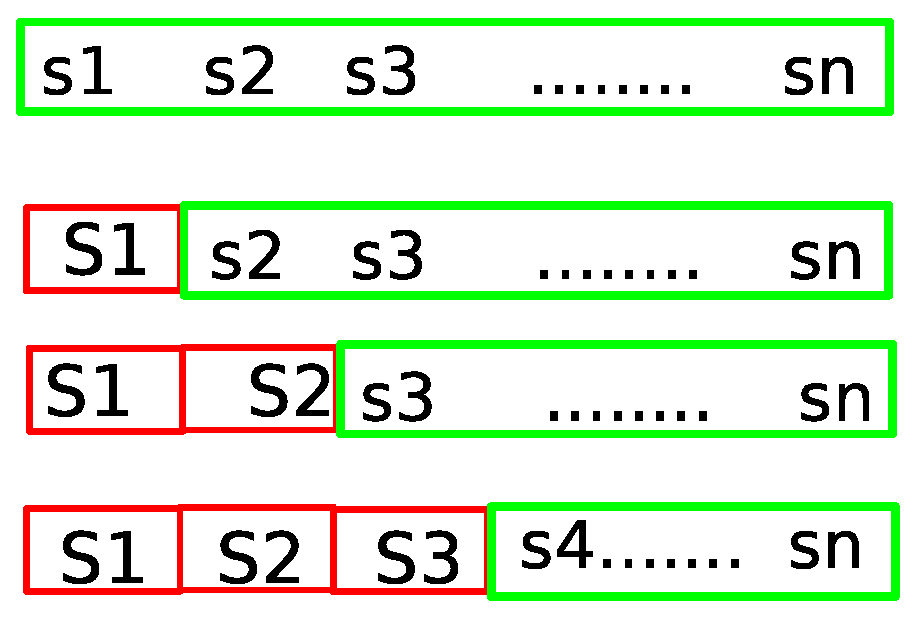
\includegraphics[width=3in] {L7-incremental-dc.eps}
%\end{figure}
%}

\frame{
	\frametitle{Greedy technique }
	\begin{itemize}
	
		 \item Greedy technique typically applies to the \textcolor{red}{\bf optimization problems} if: 
	 	\begin{enumerate}
			\item The original problem can be divided into smaller subproblems. 
			\item The recursion among sub-problems can be represented as \textcolor{red}{\bf optimal-substructure property}: the optimal solution to the original problem can be calculated through \textcolor{red}{\bf combining the optimal solutions to subproblems}. 
			\item We can design a \textcolor{red}{\bf greedy-selection rule} to select a certain sub-problem at a stage. 
		\end{enumerate}
		 \item In particular, greedy is usually used to solve an optimization problem whose solving process can be described as a multistage decision process, e.g., solution has the form $X=[x_1, x_2,..., x_n]$, $x_i = 0/1$. 
		\item  For this type of problems, we can construct \textcolor{red}{\bf  a tree to enumerate all possible  decisions}, and greedy technique can be treated as finding \textcolor{red}{\bf a set of paths} from root (null solution) to a leaf node (complete solution). At each intermediate node, greedy rule is applied to select one of its children nodes. 
	\end{itemize}
}

\frame{
\begin{block}{}
 The first example: Two versions of {\sc IntervalScheduling} problem
\end{block}
}


\frame{
\frametitle{{\sc IntervalScheduling} problem }
\begin{itemize} 
	\item Practical problem: 
	\begin{itemize}
		\item A class room is requested by several courses; 
		\item The $i$-th course $A_i$ starts from  $S_i$ and ends at $F_i$.
	\end{itemize}
	\item  Objective: to meet as many students as possible. 
 \end{itemize}
 } 
 
\frame{
\frametitle{An instance } 

%\begin{figure}
% \includegraphics[width=4in] {L7-intervalschedulingexample.eps}
%\end{figure}

\begin{figure}[!ht]
  \centering
  \begin{tikzpicture}
  [dot/.style={circle,draw=black,fill=black,thick,inner sep=0pt,minimum size=1mm}]
  \node[dot] (11) at (0.2,0.3) {};
  \node[dot,label=above:{\tiny $A_2$}] (12) at (2,0.3) {};
  \node[dot] (13) at (3,0.3) {};
  \node[dot,label=above:{\tiny $A_4$}] (14) at (4,0.3) {};
  \node[dot] (15) at (5,0.3) {};
  \node[dot,label=above:{\tiny $A_7$}] (16) at (7,0.3) {};
  \node[dot] (17) at (8.5,0.3) {};
  \node[dot,label=above:{\tiny $A_8$}] (18) at (9,0.3) {};
  
  \node[dot] (21) at (0.15,1.1) {};
  \node[dot,label=above:{\tiny $A_1$}] (22) at (1.3,1.1) {};
  \node[dot] (23) at (1.8,1.1) {};
  \node[dot,label=above:{\tiny $A_3$}] (24) at (3.5,1.1) {};
  \node[dot] (25) at (4.6,1.1) {};
  \node[dot,label=above:{\tiny $A_5$}] (26) at (6,1.1) {};
  \node[dot] (27) at (7.8,1.1) {};
  \node[dot,label=above:{\tiny $A_9$}] (28) at (9.4,1.1) {};
  
  \node[dot] (31) at (0.2,1.9) {};
  \node[dot,label=above:{\tiny $A_6$}] (32) at (6.5,1.9) {};
  
  \draw [black,thick] (11) -- (12)node [midway,above,draw=none] {\textcolor[rgb]{1.00,0.00,0.00}{\tiny {$W_2=5$}}};
  \draw [black,thick] (13)node [above,draw=none] {\textcolor[rgb]{1.00,0.00,0.00}{\tiny {{$W_4=2$}}}} -- (14);
  \draw [black,thick] (15) -- (16) node [midway,above,draw=none] {\textcolor[rgb]{1.00,0.00,0.00}{\tiny {{$W_7=1$}}}};
  \draw [black,thick] (17) -- (18);
  
  \draw [white] (8.2,0.38) node [above,draw=none] {\textcolor[rgb]{1.00,0.00,0.00}{\tiny {{$W_8=3$}}}}-- (9,0.38);
  
  \draw [black,thick] (21)node [above,draw=none] {\textcolor[rgb]{1.00,0.00,0.00}{\tiny {$W_1=1$}}} -- (22);
  \draw [black,thick] (23) --node [above,draw=none] {\textcolor[rgb]{1.00,0.00,0.00}{\tiny {$W_3=4$}}} (24);
  \draw [black,thick] (25) node [above,draw=none] {\textcolor[rgb]{1.00,0.00,0.00}{\tiny {$W_5=3$}}}-- (26);
  \draw [black,thick] (27) node [above,draw=none] {\textcolor[rgb]{1.00,0.00,0.00}{\tiny {{$W_9=5$}}}}-- (28);
  
  \draw [black,thick] (31) -- (32) node [midway,above,draw=none] {\textcolor[rgb]{1.00,0.00,0.00}{\tiny {$W_6=2$}}};
  
  \draw [->,green,thick] (0,0) -- (9.5,0) node [right,draw=none] {\textcolor[rgb]{0.00,0.00,0.00}{$Time$}};
  \end{tikzpicture}
%  \caption{L7-intervalschedulingexample.eps}
\end{figure}

\begin{eqnarray}  \nonumber
\texttt{Solutions:} & S_1=\{ A_1, A_3, A_5, A_8 \} &|\quad S_2= \{ A_6, A_9 \}  \nonumber \\
\texttt{Benefits:} &  B(S_1)=1+4+3+3=11 &|\quad  B(S_2)=2+5=7   \nonumber 
\end{eqnarray} \nonumber
}

 
\frame{
\frametitle{{\sc IntervalScheduling} problem: version 1 }
 

\begin{block}{}
{\bf INPUT: }  \\
  $n$ activities $A=\{A_1, A_2, ..., A_n \}$ that wish to use a resource. Each activity $A_i$ uses the resource during interval $[S_i, F_i)$. The selection of activity $A_i$ yields a benefit of $W_i$.\\
{\bf OUTPUT: } \\ 
 To select a collection of \textcolor{blue}{\bf compatible} activities to \textcolor{red}{\bf maximize benefits}.  
\end{block}

 	\begin{itemize}
		\item Here, $A_i$ and $A_j$ are \textcolor{blue}{\bf compatible} if there is no overlap between the corresponding intervals $[S_i, F_i)$ and $[S_j, F_j)$, i.e. the resource cannot be used by more than one activities at a time.
		\item It is assumed that the activities have been sorted according to the finishing time, i.e. $F_i \leq F_j$ for any $i < j$. 
	\end{itemize}
}


\frame[allowframebreaks]{
\frametitle{Defining general form of subproblems}
\begin{itemize}
\item It is not easy to solve a problem with $n$ activities directly. Let's see whether it can be reduced into smaller sub-problems. 
\item Solution: a subset of activities. Let's describe the solving process as a series of decisions:  at each  decision step, an activity was chosen to use the resource.  
\item Suppose we have already worked out the optimal solution. Consider \textcolor{red}{\bf the first  decision} in the optimal solution, i.e. whether $A_n$ is selected or not. There are $2$ options: 
\ \\
\begin{enumerate}
 \item Select activity $A_n$: the selection leads to a  \textcolor{red}{\bf smaller subproblem}, namely selecting from the activities ending before $S_n$. 
% 
% \begin{figure}
% 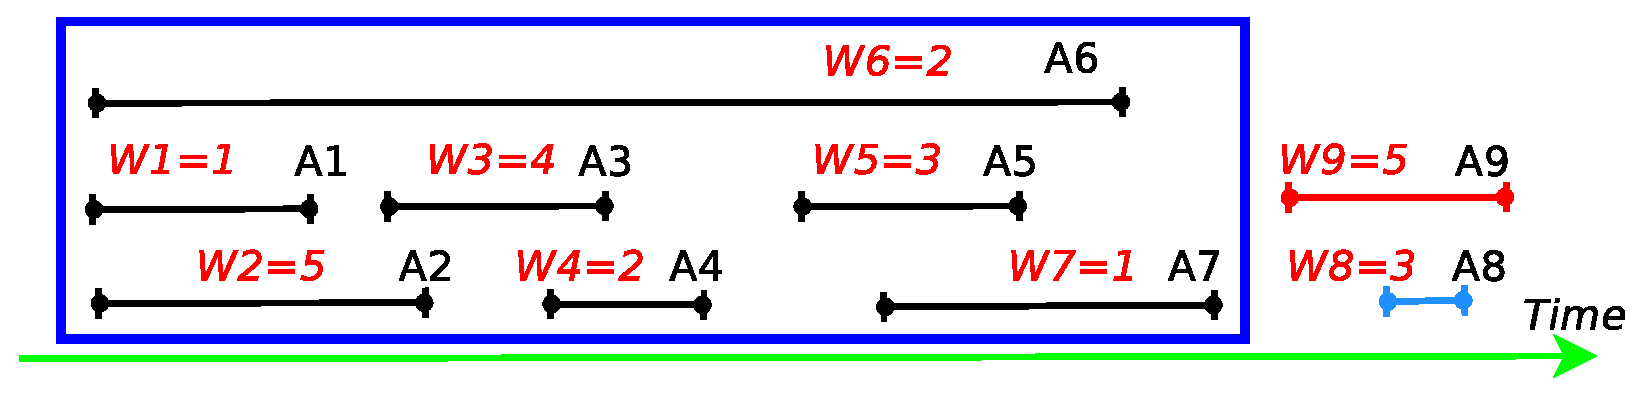
\includegraphics[width=3in] {L7-intervalschedulingexamplek1.eps}
%\end{figure}
\begin{figure}[!ht]
  \centering
  \begin{tikzpicture}
  [scale=0.7,dot/.style={circle,draw=black,fill=black,thick,inner sep=0pt,minimum size=1mm},
  bluedot/.style={circle,draw=blue,fill=blue,thick,inner sep=0pt,minimum size=1mm},
  reddot/.style={circle,draw=red,fill=red,thick,inner sep=0pt,minimum size=1mm}]
  \node[dot] (11) at (0.2,0.3) {};
  \node[dot,label=above:{\tiny $A_2$}] (12) at (2,0.3) {};
  \node[dot] (13) at (3,0.3) {};
  \node[dot,label=above:{\tiny $A_4$}] (14) at (4,0.3) {};
  \node[dot] (15) at (5,0.3) {};
  \node[dot,label=above:{\tiny $A_7$}] (16) at (7,0.3) {};
  \node[bluedot] (17) at (8.5,0.3) {};
  \node[bluedot,label=above:{\tiny $A_8$}] (18) at (9,0.3) {};
  
  \node[dot] (21) at (0.15,1.1) {};
  \node[dot,label=above:{\tiny $A_1$}] (22) at (1.3,1.1) {};
  \node[dot] (23) at (1.8,1.1) {};
  \node[dot,label=above:{\tiny $A_3$}] (24) at (3.5,1.1) {};
  \node[dot] (25) at (4.6,1.1) {};
  \node[dot,label=above:{\tiny $A_5$}] (26) at (6,1.1) {};
  \node[reddot] (27) at (7.8,1.1) {};
  \node[reddot,label=above:{\tiny $A_9$}] (28) at (9.4,1.1) {};
  
  \node[dot] (31) at (0.2,1.9) {};
  \node[dot,label=above:{\tiny $A_6$}] (32) at (6.5,1.9) {};
  
  \draw [black,thick] (11) -- (12)node [midway,above,draw=none] {\textcolor[rgb]{1.00,0.00,0.00}{\tiny {$W_2=5$}}};
  \draw [black,thick] (13)node [above,draw=none] {\textcolor[rgb]{1.00,0.00,0.00}{\tiny {{$W_4=2$}}}} -- (14);
  \draw [black,thick] (15) -- (16) node [midway,above,draw=none] {\textcolor[rgb]{1.00,0.00,0.00}{\tiny {{$W_7=1$}}}};
  \draw [blue,thick] (17) -- (18);
  
  \draw [white] (8.2,0.38) node [above,draw=none] {\textcolor[rgb]{1.00,0.00,0.00}{\tiny {{$W_8=3$}}}}-- (9,0.38);
  
  \draw [black,thick] (21)node [above,draw=none] {\textcolor[rgb]{1.00,0.00,0.00}{\tiny {$W_1=1$}}} -- (22);
  \draw [black,thick] (23) --node [above,draw=none] {\textcolor[rgb]{1.00,0.00,0.00}{\tiny {$W_3=4$}}} (24);
  \draw [black,thick] (25) node [above,draw=none] {\textcolor[rgb]{1.00,0.00,0.00}{\tiny {$W_5=3$}}}-- (26);
  \draw [red,thick] (27) node [above,draw=none] {\textcolor[rgb]{1.00,0.00,0.00}{\tiny {{$W_9=5$}}}}-- (28);
  
  \draw [black,thick] (31) -- (32) node [midway,above,draw=none] {\textcolor[rgb]{1.00,0.00,0.00}{\tiny {$W_6=2$}}};
  
  \draw [->,green,thick] (0,0) -- (9.5,0) node [right,draw=none] {\textcolor[rgb]{0.00,0.00,0.00}{$Time$}};
  
  \draw [blue,thick,line width=0.05cm] (-0.5,0.15) -- (7.3,.15) -- (7.3,2.5) -- (-0.5,2.5) -- (-0.5,0.15);
  \end{tikzpicture}
%  \caption{L7-intervalschedulingexamplek1.eps}
\end{figure}

 \item Abandon activity $A_n$: then it suffices to solve another \textcolor{red}{\bf smaller subproblem}: to select activities from $A_1, A_2, ..., A_{n-1}$. 

\begin{figure}[!ht]
  \centering
  \begin{tikzpicture}
  [scale=0.7,dot/.style={circle,draw=black,fill=black,thick,inner sep=0pt,minimum size=1mm},
  bluedot/.style={circle,draw=blue,fill=blue,thick,inner sep=0pt,minimum size=1mm},
  reddot/.style={circle,draw=red,fill=red,thick,inner sep=0pt,minimum size=1mm}]
  \node[dot] (11) at (0.2,0.3) {};
  \node[dot,label=above:{\tiny $A_2$}] (12) at (2,0.3) {};
  \node[dot] (13) at (3,0.3) {};
  \node[dot,label=above:{\tiny $A_4$}] (14) at (4,0.3) {};
  \node[dot] (15) at (5,0.3) {};
  \node[dot,label=above:{\tiny $A_7$}] (16) at (7,0.3) {};
  \node[dot] (17) at (8.5,0.3) {};
  \node[dot,label=above:{\tiny $A_8$}] (18) at (9,0.3) {};
  
  \node[dot] (21) at (0.15,1.1) {};
  \node[dot,label=above:{\tiny $A_1$}] (22) at (1.3,1.1) {};
  \node[dot] (23) at (1.8,1.1) {};
  \node[dot,label=above:{\tiny $A_3$}] (24) at (3.5,1.1) {};
  \node[dot] (25) at (4.6,1.1) {};
  \node[dot,label=above:{\tiny $A_5$}] (26) at (6,1.1) {};
  \node[bluedot] (27) at (7.8,1.1) {};
  \node[bluedot,label=above:{\tiny $A_9$}] (28) at (9.4,1.1) {};
  
  \node[dot] (31) at (0.2,1.9) {};
  \node[dot,label=above:{\tiny $A_6$}] (32) at (6.5,1.9) {};
  
  \draw [black,thick] (11) -- (12)node [midway,above,draw=none] {\textcolor[rgb]{1.00,0.00,0.00}{\tiny {$W_2=5$}}};
  \draw [black,thick] (13)node [above,draw=none] {\textcolor[rgb]{1.00,0.00,0.00}{\tiny {{$W_4=2$}}}} -- (14);
  \draw [black,thick] (15) -- (16) node [midway,above,draw=none] {\textcolor[rgb]{1.00,0.00,0.00}{\tiny {{$W_7=1$}}}};
  \draw [black,thick] (17) -- (18);
  
  \draw [white] (8.2,0.38) node [above,draw=none] {\textcolor[rgb]{1.00,0.00,0.00}{\tiny {{$W_8=3$}}}}-- (9,0.38);
  
  \draw [black,thick] (21)node [above,draw=none] {\textcolor[rgb]{1.00,0.00,0.00}{\tiny {$W_1=1$}}} -- (22);
  \draw [black,thick] (23) --node [above,draw=none] {\textcolor[rgb]{1.00,0.00,0.00}{\tiny {$W_3=4$}}} (24);
  \draw [black,thick] (25) node [above,draw=none] {\textcolor[rgb]{1.00,0.00,0.00}{\tiny {$W_5=3$}}}-- (26);
  \draw [blue,thick] (27) node [above,draw=none] {\textcolor[rgb]{1.00,0.00,0.00}{\tiny {{$W_9=5$}}}}-- (28);
  
  \draw [black,thick] (31) -- (32) node [midway,above,draw=none] {\textcolor[rgb]{1.00,0.00,0.00}{\tiny {$W_6=2$}}};
  
  \draw [->,green,thick] (0,0) -- (9.5,0) node [right,draw=none] {\textcolor[rgb]{0.00,0.00,0.00}{$Time$}};
  
  \draw [blue,thick,line width=0.05cm] (-0.5,0.15) -- (9.1,.15) -- (9.1,2.5) -- (-0.5,2.5) -- (-0.5,0.15);
  \end{tikzpicture}
  %\caption{L7-intervalschedulingexamplek2.eps}
\end{figure}

%  \begin{figure}
% \includegraphics[width=3in] {L7-intervalschedulingexamplek2.eps}
%\end{figure}
 \end{enumerate}

\end{itemize}
} 


\frame{
\frametitle{Optimal sub-structure property}
% \begin{figure}
% 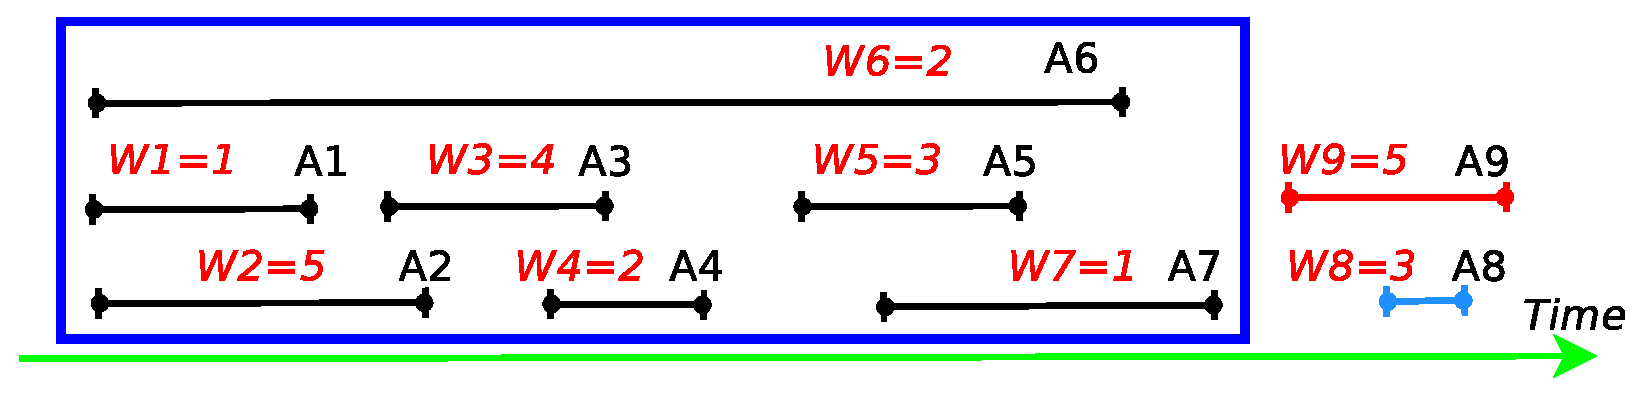
\includegraphics[width=4in] {L7-intervalschedulingexamplek1.eps}
%\end{figure}
%
%  \begin{figure}
% \includegraphics[width=4in] {L7-intervalschedulingexamplek2.eps}
%\end{figure}


\begin{itemize}
\item Summarizing the two cases,  we can design the general form of subproblems as: 
\textcolor{red}{ {\bf selecting a collection of activities from $A_1, A_2, ..., A_i$ to maximize benefits}}.  Let's denote the optimal solution value as $OPT(i)$. 

%\footnote{  $A_{i..j} = \phi$ whenever $i\geq j$. Here we suppose that  all $A_i$ were sorted in increasing order of finish time, and $A_0$ and $A_{10}$ are introduced as a sentinels. }
%\item Intuition of $A_{i..j}$: the activities begin after $A_i$ ends and end before $A_j$ starts. 

%\item Intuition of $A_{i..j}$: the activities begin after $A_i$ ends and end before $A_j$ starts. 
\item Optimal substructure property: (``cut-and-paste'' argument)
\[
OPT(i) = \max \begin{cases}
        OPT( pre(i) ) + W_i \nonumber \\ 
  	OPT( i-1) \nonumber 
  \end{cases} 
\]
Here, $pre(i)$ denotes the largest index of the activities ending before $S_i$. 
\end{itemize}
}



\frame{
\frametitle{Dynamic programming algorithm} 
\begin{footnotesize}
{\sc Recursive\_DP}$( i )$
\begin{algorithmic}[1]
\REQUIRE{ All $A_i$ have been sorted in the increasing order of $F_i$.}
\IF { $i \leq 0$ } 
	\RETURN $0$; 
\ENDIF
\IF { $i == 1$ } 
	\RETURN $W_1$; 
\ENDIF
\STATE Let $pre(i)$ denotes the largest index of the activities ending before $S_i$ 
\STATE $m=  \max \begin{cases}
        \text{\sc Recursive\_DP}( pre(i) ) + W_i \nonumber \\ 
  	\text{\sc Recursive\_DP}( i-1) \nonumber 
  \end{cases} $  
\RETURN $m$;
\end{algorithmic}
\end{footnotesize}
\begin{itemize}
\item The original problem can be solved by calling {\sc Recursive\_DP}$(n)$. 
\item It needs $O(n \log n)$ to sort the activities and determine $pre(.)$, and the dynamic programming needs $O(n)$ time.  Thus, the total running time is  $O(n \log n)$
\end{itemize}
}

\frame{
	\frametitle{multistage decision process} 

\begin{figure}
\begin{tikzpicture}[scale=1., auto,swap]
    % Draw a 7,11 network
    % First we draw the vertices
    \foreach \pos/\name/\label in {{(0,0)/root/}, 
    {(-3,-1)/L/}, {(3,-1)/R/}}
        \node[tinyvertex,draw=black, fill=white!20] (\name) at \pos {};
        
        
        \foreach \pos/\name/\label in {{(0.1,0)/root/P_0:\ X=[?,?,?,?,?,?,?,?,?]}, 
    {(-2.9,-1)/L/P_1:\ X=[?,?,?,?,?,?,?,?,1]}, {(3.1,-1)/R/P_2:\ X=[?,?,?,?,?,?,?,?,0]}}
        \node[right] at \pos {\tiny $\label$};    

    % Connect vertices with edges and draw weights
  \foreach \source/ \dest /\weight in {root/L/{\tiny x_9=1}, R/root/{\tiny x_9=0}}
        \path[undirectededge] (\source) -- node[ weight] {$\weight$} (\dest);
%       \draw[dashed, ->] (0,0) arc  (120:60:2);
 
   \end{tikzpicture}
\end{figure}

\begin{itemize}
	\item Here we represent a solution as $X=[x_1, x_2, ..., x_9]$, where $x_i=1$ denotes the selection of activity $A_i$ and abandon otherwise. 
	\item At the first decision step, we have to enumerate both options $x_9 = 0$ and $x_9 = 1$ as we have no idea  which one is optimal.  
\end{itemize}

}


\frame{
\frametitle{A more cumbersome dynamic programming algorithm} 
\begin{itemize}
\item It is not easy to solve a problem with $n$ activities directly. Let's see whether it can be reduced into smaller sub-problems. 
\item Solution: a subset of activities. Let's describe the solving process as a series of decisions:  at each  decision step, an activity is chosen to use the resource.  
\item Suppose we have already worked out the optimal solution. Consider \textcolor{red}{\bf the first  decision} in the optimal solution, i.e. a certain activity $A_i$ is selected. There are at most $n$ options: 
\begin{itemize}
 \item Select an activity $A_i$: the selection leads to a  \textcolor{red}{\bf smaller subproblem}, namely, selecting from the activity set with $A_i$ and the activities conflicting with $A_i$ removed. 
% 
% \begin{figure}
% 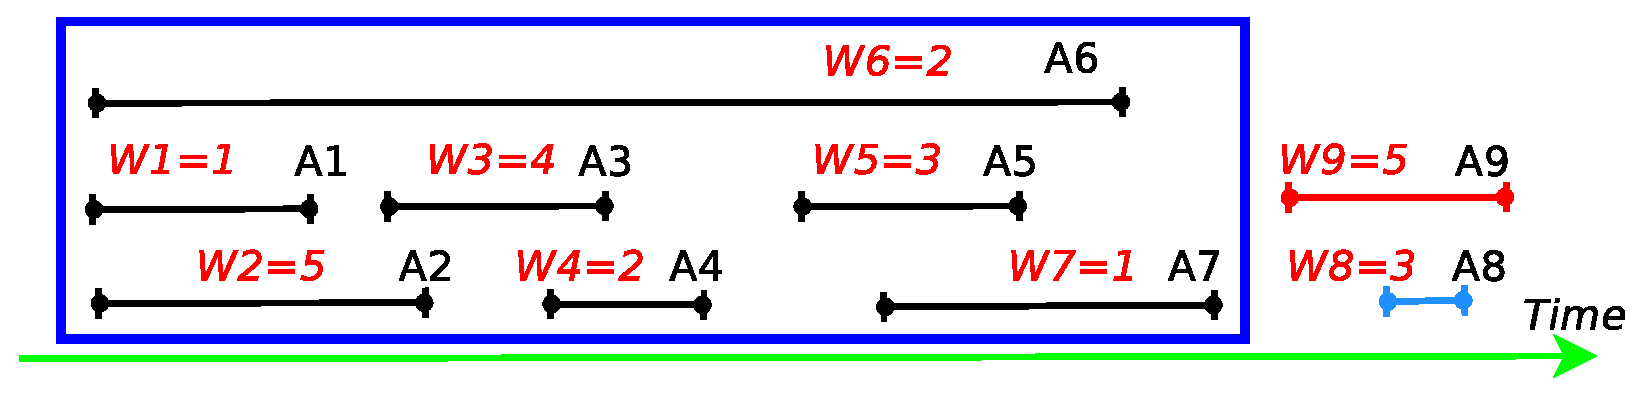
\includegraphics[width=3in] {L7-intervalschedulingexamplek1.eps}
%\end{figure}
\begin{figure}[!ht]
  \centering
  \begin{tikzpicture}
  [scale=0.7,dot/.style={circle,draw=black,fill=black,thick,inner sep=0pt,minimum size=1mm},
  bluedot/.style={circle,draw=blue,fill=blue,thick,inner sep=0pt,minimum size=1mm},
  reddot/.style={circle,draw=red,fill=red,thick,inner sep=0pt,minimum size=1mm}]
  \node[dot] (11) at (0.2,0.3) {};
  \node[dot,label=above:{\tiny $A_2$}] (12) at (2,0.3) {};
  \node[dot] (13) at (3,0.3) {};
  \node[dot,label=above:{\tiny $A_4$}] (14) at (4,0.3) {};
  \node[dot] (15) at (5,0.3) {};
  \node[dot,label=above:{\tiny $A_7$}] (16) at (7,0.3) {};
  \node[dot] (17) at (8.5,0.3) {};
  \node[dot,label=above:{\tiny $A_8$}] (18) at (9,0.3) {};
  
  \node[dot] (21) at (0.15,1.1) {};
  \node[dot,label=above:{\tiny $A_1$}] (22) at (1.3,1.1) {};
  \node[dot] (23) at (1.8,1.1) {};
  \node[dot,label=above:{\tiny $A_3$}] (24) at (3.5,1.1) {};
  \node[dot] (25) at (4.6,1.1) {};
  \node[dot,label=above:{\tiny $A_5$}] (26) at (6,1.1) {};
  \node[dot] (27) at (7.8,1.1) {};
  \node[dot,label=above:{\tiny $A_9$}] (28) at (9.4,1.1) {};
  
  \node[dot] (31) at (0.2,1.9) {};
  \node[dot,label=above:{\tiny $A_6$}] (32) at (6.5,1.9) {};
  
  \draw [black,thick] (11) -- (12)node [midway,above,draw=none] {\textcolor[rgb]{1.00,0.00,0.00}{\tiny {$W_2=5$}}};
  \draw [black,thick] (13)node [above,draw=none] {\textcolor[rgb]{1.00,0.00,0.00}{\tiny {{$W_4=2$}}}} -- (14);
  \draw [blue] (15) -- (16) node [midway,above,draw=none] {\textcolor[rgb]{1.00,0.00,0.00}{\tiny {{$W_7=1$}}}};
  \draw [black,thick] (17) -- (18);
  
  \draw [white] (8.2,0.38) node [above,draw=none] {\textcolor[rgb]{1.00,0.00,0.00}{\tiny {{$W_8=3$}}}}-- (9,0.38);
  
  \draw [black,thick] (21)node [above,draw=none] {\textcolor[rgb]{1.00,0.00,0.00}{\tiny {$W_1=1$}}} -- (22);
  \draw [black,thick] (23) --node [above,draw=none] {\textcolor[rgb]{1.00,0.00,0.00}{\tiny {$W_3=4$}}} (24);
  \draw [red,thick] (25) node [above,draw=none] {\textcolor[rgb]{1.00,0.00,0.00}{\tiny {$W_5=3$}}}-- (26);
  \draw [black,thick] (27) node [above,draw=none] {\textcolor[rgb]{1.00,0.00,0.00}{\tiny {{$W_9=5$}}}}-- (28);
  
  \draw [blue] (31) -- (32) node [midway,above,draw=none] {\textcolor[rgb]{1.00,0.00,0.00}{\tiny {$W_6=2$}}};
  
  \draw [->,green,thick] (0,0) -- (9.5,0) node [right,draw=none] {\textcolor[rgb]{0.00,0.00,0.00}{$Time$}};
  
%  \draw [blue,thick,line width=0.05cm] (-0.5,0.15) -- (7.3,.15) -- (7.3,2.5) -- (-0.5,2.5) -- (-0.5,0.15);
  \end{tikzpicture}
%  \caption{L7-intervalschedulingexamplek1.eps}
\end{figure}


%  \begin{figure}
% \includegraphics[width=3in] {L7-intervalschedulingexamplek2.eps}
%\end{figure}
 \end{itemize}

\end{itemize}
} 


\frame{
\frametitle{Optimal sub-structure property}
% \begin{figure}
% 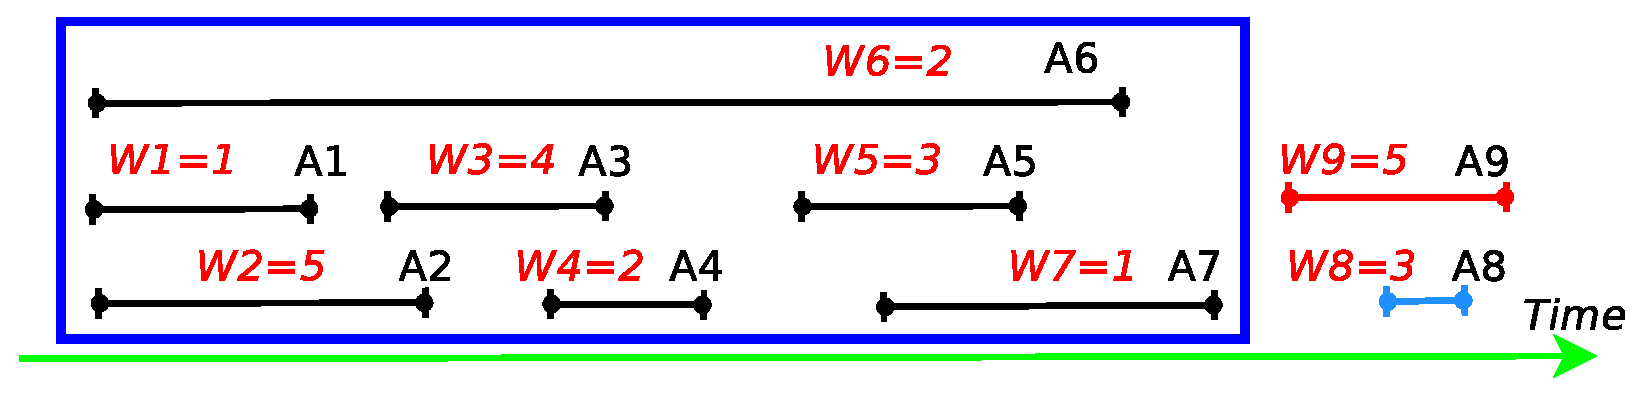
\includegraphics[width=4in] {L7-intervalschedulingexamplek1.eps}
%\end{figure}
%
%  \begin{figure}
% \includegraphics[width=4in] {L7-intervalschedulingexamplek2.eps}
%\end{figure}


\begin{itemize}
\item Summarizing these cases,  we can design the general form of subproblems as: 
\textcolor{red}{{\bf selecting a collection of activities from a subset $S$ ($S\subseteq \{A_1, A_2, ..., A_n\}$) to maximize benefits}}.  Let's denote the optimal solution value as $OPT(S)$. 

%\footnote{  $A_{i..j} = \phi$ whenever $i\geq j$. Here we suppose that  all $A_i$ were sorted in increasing order of finish time, and $A_0$ and $A_{10}$ are introduced as a sentinels. }
%\item Intuition of $A_{i..j}$: the activities begin after $A_i$ ends and end before $A_j$ starts. 

%\item Intuition of $A_{i..j}$: the activities begin after $A_i$ ends and end before $A_j$ starts. 
\item Optimal substructure property: (``cut-and-paste'' argument)
\[
OPT(S) = \max_{A_i \in S}\{OPT( R(S, A_i) ) + W_i\}
\]
Here, $R(S, A_i)$ represents the subset with $A_i$ and the activities conflicting with $A_i$ removed from $S$. 
\end{itemize}
}

\frame{
\frametitle{Dynamic programming algorithm} 
\begin{footnotesize}
{\sc Recursive\_DP}$( S )$
\begin{algorithmic}[1]
\IF{$S$ is empty} 
	\RETURN $0$; 
\ENDIF
\STATE{$m=0$}; 
\FORALL{activity $A_i \in S$}
	\STATE{Set $S'$ as the subset with $A_i$ and the activities conflicting with $A_i$ removed from $S$}; 
	\IF{$m < ${\sc Recursive\_DP}$(S') + W_i$}
		\STATE{$m = {\sc Recursive\_DP}(S') + W_i$};
	\ENDIF
\ENDFOR
\RETURN $m$;
\end{algorithmic}
\end{footnotesize}
\begin{itemize}
\item The original problem can be solved by calling {\sc Recursive\_DP}$(\{A_1, A_2, ..., A_n\})$. 
\item The total running time is  $O(2^n)$ as the number of subproblems is exponential. 
\end{itemize}
}

\frame{
	\frametitle{Multistage decision process}
\begin{figure}
\begin{tikzpicture}[scale=0.8, auto,swap]

    \def\dx{0};
   \def\dy{0.9} 
%    \foreach \pos/ \name in {{(-1.8+\dx,0+\dy)/a},{(1.8+\dx,0+\dy)/b}, {(-0.9+\dx,1.3+\dy)/e}, {(0.9+\dx,1.3+\dy)/c}, {(0+\dx,2.6+\dy)/d}}         
%    	\node[smallvertex,fill=blue!20] (\name) at \pos{$\name$};
%     
%    % Connect vertices with edges and draw weights
%     %   \foreach \source/ \dest/\weight in {a/b/{3},   c/a/{4}, e/a/{7}, a/d/{2}, b/c/{4}, b/d/{6}, e/b/{3}, c/d/{5}, c/e/{8}, d/e/{6}}
%    \foreach \source/ \dest/\weight in {a/b/{e_1{:}\ 3},   a/c/{}, e/a/{e_{5}{:}\  7}, b/c/{e_{4}{:}\  4}, b/e/{}, c/d/, c/e/{e_{9}{:}\  8}, d/e/}
%        \path[undirectededge] (\source) -- node[weight] {\tiny $\weight$} (\dest);
%         
%    \draw[thick] (a)   to [out=140, in=180] node[left] {\tiny $e_{3}{:}\  2$} (d);   
%        \draw[thick] (b)   to [out=40, in=0] node[right] {\tiny $e_{6}{:}\  6$} (d);   
%        
%       \foreach \source/ \dest/\weight in {a/b/,   b/c/,  c/d/, d/e/, e/a/}
%        \path[undirectededge] (\source) -- node[weight] {$\weight$} (\dest);
%/Users/dbu/Library/Mobile Documents/com~apple~CloudDocs/images.jpeg
%   \node[] at (-0.7+\dx, 0.3+\dy) {\tiny $e_{2}{:}\  4$}; 
%   \node[] at (0.7+\dx, 0.3+\dy) {\tiny $e_{7}{:}\  3$}; 
%  \node[] at (-0.9+\dx, 2.0+\dy) {\tiny $e_{10}{:}\  6$}; 
%  \node[] at (0.9+\dx, 2.0+\dy) {\tiny $e_{8}{:}\  5$}; 
 
%Tree

	\def\d{2.4}; 
	\def\e{1.5};
	\def\f{1.0};
	\def\h{1.5};

% Label
	
   \node at ( -1.5*\d - 2*\e, -\h * 0.5)  {\tiny $x_1=A_1/A_2/.../A_9$};  

%layer 1	
    \foreach \pos/\name/\label in {{(0,0)/root/}} 
        \node[tinyvertex,draw=black, fill=white!20] (\name) at \pos {};
%layer 2	
    \foreach \pos/\name/\label in { {(-1.5*\d, -1*\h)/L11/}, {(-0.5*\d,-1*\h)/L12/}, {(1.5*\d, -1*\h)/L14/}}  
        \node[tinyvertex,draw=black, fill=white!20] (\name) at \pos {};	

            
 % Edges 
 	%layer 1
  	\foreach \source/ \dest /\weight in {root/L11/, root/L12/, root/L14/ }         
		\path[undirectededge] (\source) -- node[weight] { } (\dest);

   %Label
   \def\s{1.05};  
   \def\t{0.3};  
   \node[] at (0 + \s, 0) {\tiny $X=[??...?]$}; 
   \node[] at (0 + \s, 0 - \t) {\tiny ${\tiny P_{0}}$}; 
 
  %layer 1
    \def\s{0.75};  
   \node[] at (-1.5*\d + \s, -1*\h-\t ) {\tiny $X=[A_1?...?]$}; 
   \node[] at (-1.5*\d + \s, -1*\h-\t  - \t) {\tiny ${\tiny P_{1}}$ }; 

   \node[] at (-0.5*\d + \s, -1*\h-\t ) {\tiny $X=[A_2?...?]$}; 
   \node[] at (-0.5*\d + \s, -1*\h-\t  - \t) {\tiny ${\tiny P_{2}}$ }; 
  
  \node[] at (0.25*\d + \s, -0.5*\h-\t ) {......};
  
%   \node[] at (0.5*\d + \s, -1*\h-\t ) {\tiny $A_8$?...?}; 
%   \node[] at (0.5*\d + \s, -1*\h-\t  - \t) {\tiny ${\tiny P_{8}}$ }; 

   \node[] at (1.5*\d + \s, -1*\h-\t ) {\tiny $X=[A_9?...?]$  }; 
   \node[] at (1.5*\d + \s, -1*\h-\t  - \t) {\tiny ${\tiny P_{9}}$ }; 

   \end{tikzpicture}
\end{figure}

\begin{itemize}
	\item Here we represent the optimal solution as $X=[x_1, x_2, ......]$, where $x_i\in \{A_1, A_2, ..., A_9\}$ denotes the activity selected at the $i$-th decision step. 
	\item At the first decision step, we have to enumerate 9 options $x_1 = A_1$, $x_1 = A_2$, ......, $x_1 = A_9$ as we have no idea which one is optimal, i.e.,  
\[
OPT(S) = \max_{A_i \in S}\{OPT( R(S, A_i) ) + W_i\}.
\]

\end{itemize}

}


\frame{
	\begin{block}{}
	{\sc IntervalScheduling} problem: version 2
	\end{block}
}

\frame{
\frametitle{Let's investigate a special case }


\begin{figure}[!ht]
\centering
\begin{tikzpicture}
[dot/.style={circle,draw=black,fill=black,thick,inner sep=0pt,minimum size=1mm}]
\node[dot] (11) at (0.2,0.3) {};
\node[dot,label=above:{\tiny $A_2$}] (12) at (2,0.3) {};
\node[dot] (13) at (3,0.3) {};
\node[dot,label=above:{\tiny $A_4$}] (14) at (4,0.3) {};
\node[dot] (15) at (5,0.3) {};
\node[dot,label=above:{\tiny $A_7$}] (16) at (7,0.3) {};
\node[dot] (17) at (8.5,0.3) {};
\node[dot,label=above:{\tiny $A_8$}] (18) at (9,0.3) {};

\node[dot] (21) at (0.15,1.1) {};
\node[dot,label=above:{\tiny $A_1$}] (22) at (1.3,1.1) {};
\node[dot] (23) at (1.8,1.1) {};
\node[dot,label=above:{\tiny $A_3$}] (24) at (3.5,1.1) {};
\node[dot] (25) at (4.6,1.1) {};
\node[dot,label=above:{\tiny $A_5$}] (26) at (6,1.1) {};
\node[dot] (27) at (7.8,1.1) {};
\node[dot,label=above:{\tiny $A_9$}] (28) at (9.4,1.1) {};

\node[dot] (31) at (0.2,1.9) {};
\node[dot,label=above:{\tiny $A_6$}] (32) at (6.5,1.9) {};

\draw [black,thick] (11) -- (12)node [midway,above,draw=none] {\textcolor[rgb]{1.00,0.00,0.00}{\tiny {$W_2=1$}}};
\draw [black,thick] (13)node [above,draw=none] {\textcolor[rgb]{1.00,0.00,0.00}{\tiny {$W_4=1$}}} -- (14);
\draw [black,thick] (15) -- (16) node [midway,above,draw=none] {\textcolor[rgb]{1.00,0.00,0.00}{\tiny {$W_7=1$}}};
\draw [black,thick] (17) -- (18);

\draw [white] (8.2,0.38) node [above,draw=none] {\textcolor[rgb]{1.00,0.00,0.00}{\tiny {$W_8=1$}}}-- (9,0.38);

\draw [black,thick] (21)node [above,draw=none] {\textcolor[rgb]{1.00,0.00,0.00}{\tiny {$W_1=1$}}} -- (22);
\draw [black,thick] (23) --node [above,draw=none] {\textcolor[rgb]{1.00,0.00,0.00}{\tiny {$W_3=1$}}} (24);
\draw [black,thick] (25) node [above,draw=none] {\textcolor[rgb]{1.00,0.00,0.00}{\tiny {$W_5=1$}}}-- (26);
\draw [black,thick] (27) node [above,draw=none] {\textcolor[rgb]{1.00,0.00,0.00}{\tiny {$W_9=1$}}}-- (28);

\draw [black,thick] (31) -- (32) node [midway,above,draw=none] {\textcolor[rgb]{1.00,0.00,0.00}{\tiny {$W_6=1$}}};

\draw [->,green,thick] (0,0) -- (9.5,0) node [right,draw=none] {\textcolor[rgb]{0.00,0.00,0.00}{$Time$}};
\end{tikzpicture}
\end{figure}

A special case of {\sc IntervalScheduling} problem with \textcolor{red}{\bf all weights $w_i=1$}. \\

} 

\frame{
\frametitle{{\sc IntervalScheduling} problem: version 2  }

\begin{block}{}
{\bf INPUT: }  \\
  $n$ activities $A=\{A_1, A_2, ..., A_n \}$ that wish to use a resource. Each activity $A_i$ uses the resource during interval $[S_i, F_i)$. \\
{\bf OUTPUT: } \\ 
To select as many \textcolor{blue}{\bf compatible activities} as possible.
\end{block}

}

\frame{
 
\begin{block}{}
Greedy-selection property
\end{block}

}


\frame{
\frametitle{Another property: greedy-selection}

\begin{itemize}
	\item Since this is just a special case, the \textcolor{red}{\bf optimal substructure property}  still holds.
	\item Besides the optimal substructure property, the special weight setting leads to \textcolor{red}{\bf ``greedy-selection'' property}, i.e., to select as many courses as possible, we first select  the course with the earliest ending time. 
\end{itemize}


\begin{Theorem}
Suppose $A_1$ is the activity with the earliest ending time.  \textcolor{red}{\bf $A_1$ is used in an optimal solution. }
\end{Theorem}
}

\frame{
	\frametitle{Proof of the greedy-selection rule}
\begin{Proof} \\
\begin{itemize}
 	\item 
Suppose we have an optimal solution $O = \{ A_{i1}, A_{i2}, ..., A_{iT} \}$ but $A_{i1} \neq A_1$. 
	\item $A_1$ is compatible with $A_{i2}, ..., A_{iT}$ since $A_1$ ends earlier than $A_{i1}$. 
	\item Exchange argument: Construct a new subset $O' = O - \{A_{i1} \} \cup \{ A_1 \}$. It is clear that $O'$ is also an optimal solution since $| O' | = | O |$. 
\end{itemize}

%\begin{figure}
% 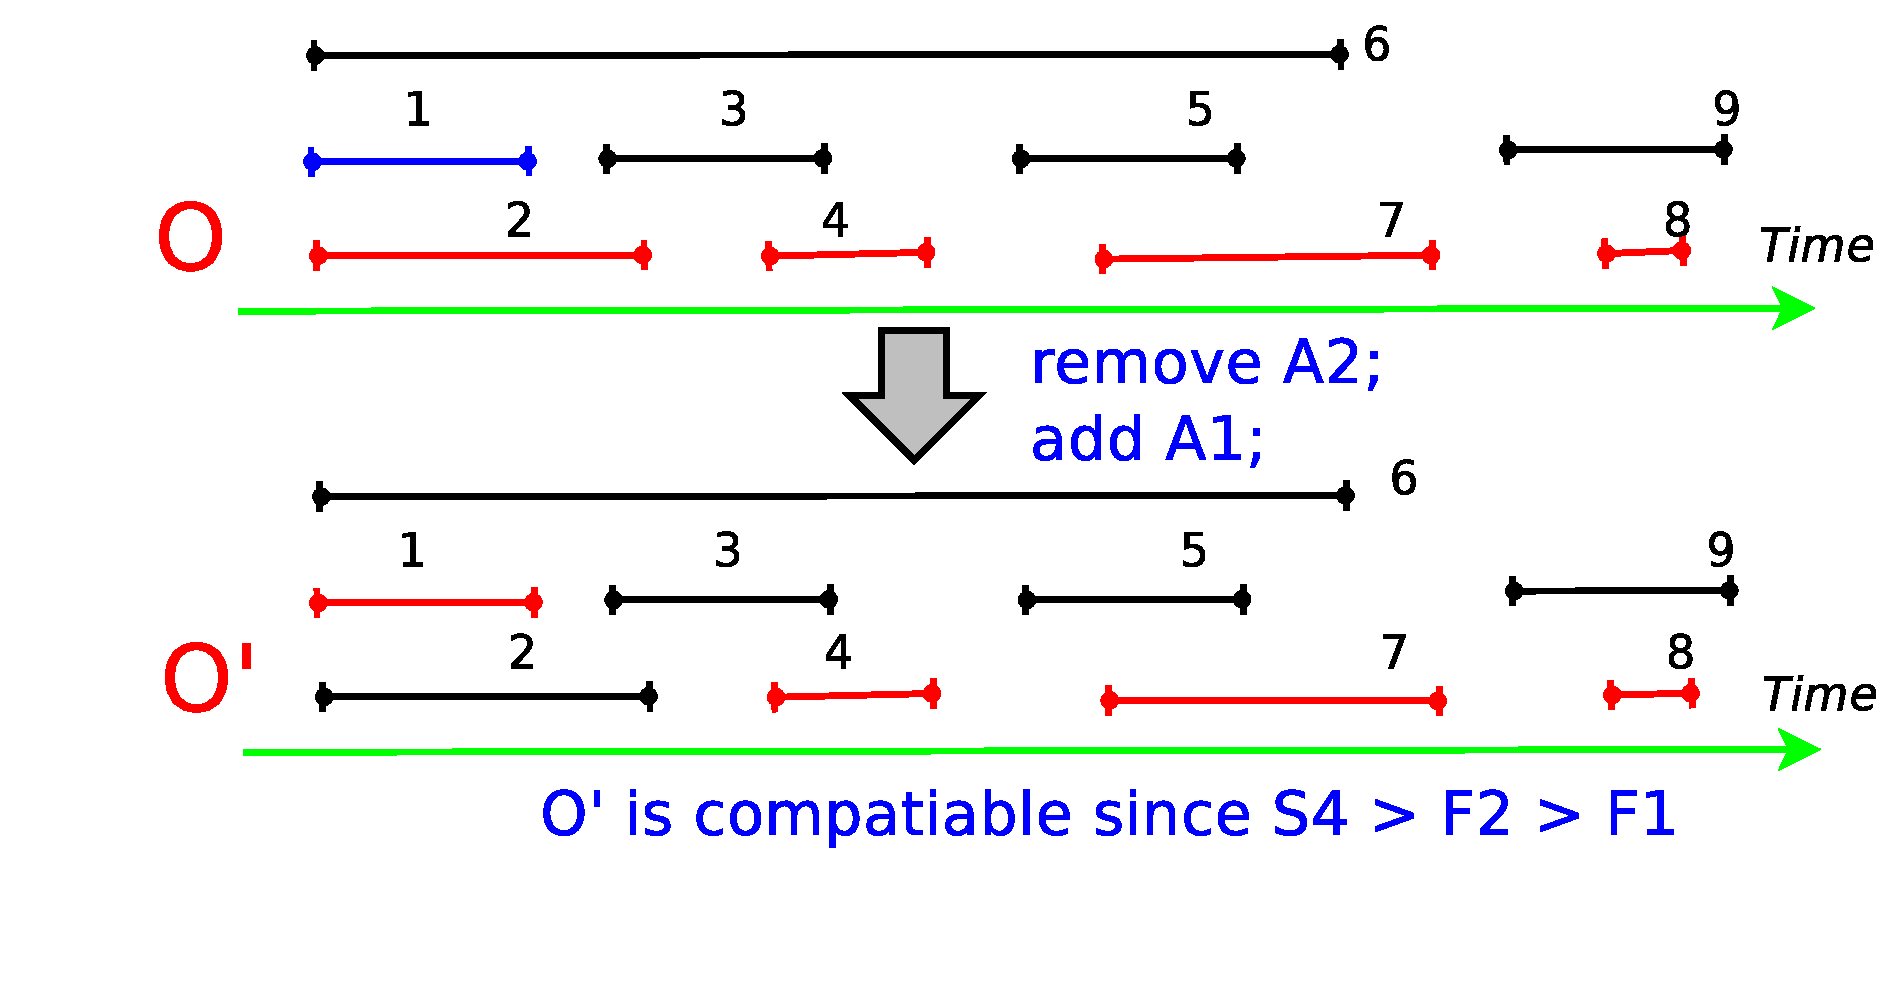
\includegraphics[width=2.9in] {L7-intervalschedulingexampleall1am.eps}
%\end{figure}
\begin{figure}[!ht]
  \centering
  \begin{tikzpicture}
  [scale=0.6, dot/.style={circle,draw=black,fill=black,thick,inner sep=0pt,minimum size=1mm},
  bluedot/.style={circle,draw=blue,fill=blue,thick,inner sep=0pt,minimum size=1mm},
  reddot/.style={circle,draw=red,fill=red,thick,inner sep=0pt,minimum size=1mm}]
  \node[dot,label=left:{\textcolor{red}{O'}}] (111) at (0.2,0.3) {};
  \node[dot] (112) at (2,0.3) {};
  \node[reddot] (113) at (3,0.3) {};
  \node[reddot] (114) at (4,0.3) {};
  \node[reddot] (115) at (5,0.3) {};
  \node[reddot] (116) at (7,0.3) {};
  \node[reddot] (117) at (8.5,0.3) {};
  \node[reddot] (118) at (9,0.3) {};
  
  \node[reddot] (121) at (0.15,1.1) {};
  \node[reddot] (122) at (1.3,1.1) {};
  \node[dot] (123) at (1.8,1.1) {};
  \node[dot] (124) at (3.5,1.1) {};
  \node[dot] (125) at (4.6,1.1) {};
  \node[dot] (126) at (6,1.1) {};
  \node[dot] (127) at (7.8,1.1) {};
  \node[dot] (128) at (9.4,1.1) {};
  
  \node[dot] (131) at (0.2,1.9) {};
  \node[dot] (132) at (6.5,1.9) {};
  
  \draw [black,thick] (111) -- (112) node [midway,above,draw=none] {\tiny $A_2$};
  \draw [red,thick] (113) -- (114) node [midway,above,draw=none] {\tiny $A_4$};
  \draw [red,thick] (115) -- (116) node [midway,above,draw=none] {\tiny $A_7$};
  \draw [red,thick] (117) -- (118) node [midway,above,draw=none] {\tiny $A_8$};
  
  \draw [red,thick] (121) -- (122) node [midway,above,draw=none] {\tiny $A_1$};
  \draw [black,thick] (123) -- (124) node [midway,above,draw=none] {\tiny $A_3$};
  \draw [black,thick] (125) -- (126) node [midway,above,draw=none] {\tiny $A_5$};
  \draw [black,thick] (127) -- (128) node [midway,above,draw=none] {\tiny $A_9$};
  
  \draw [black,thick] (131) -- (132) node [midway,above,draw=none] {\tiny $A_6$};
  
  \draw [->,green,thick] (0,0) -- (9.5,0) node [right,draw=none] {\textcolor[rgb]{0.00,0.00,0.00}{$Time$}} node [midway,below,draw=none] {\textcolor{blue}{}};
  
  
  \node[reddot,label=left:{\textcolor{red}{O}}] (211) at (0.2,3.3) {};
  \node[reddot] (212) at (2,3.3) {};
  \node[reddot] (213) at (3,3.3) {};
  \node[reddot] (214) at (4,3.3) {};
  \node[reddot] (215) at (5,3.3) {};
  \node[reddot] (216) at (7,3.3) {};
  \node[reddot] (217) at (8.5,3.3) {};
  \node[reddot] (218) at (9,3.3) {};
  
  \node[bluedot] (221) at (0.15,4.1) {};
  \node[bluedot] (222) at (1.3,4.1) {};
  \node[dot] (223) at (1.8,4.1) {};
  \node[dot] (224) at (3.5,4.1) {};
  \node[dot] (225) at (4.6,4.1) {};
  \node[dot] (226) at (6,4.1) {};
  \node[dot] (227) at (7.8,4.1) {};
  \node[dot] (228) at (9.2,4.1) {};
  
  \node[dot] (231) at (0.2,4.9) {};
  \node[dot] (232) at (6.5,4.9) {};
  
  \draw [red,thick] (211) -- (212) node [midway,above,draw=none] {\tiny $A_2$};
  \draw [red,thick] (213) -- (214) node [midway,above,draw=none] {\tiny $A_4$};
  \draw [red,thick] (215) -- (216) node [midway,above,draw=none] {\tiny $A_7$};
  \draw [red,thick] (217) -- (218) node [midway,above,draw=none] {\tiny $A_8$};
  
  \draw [blue,thick] (221) -- (222) node [midway,above,draw=none] {\tiny $A_1$};
  \draw [black,thick] (223) -- (224) node [midway,above,draw=none] {\tiny $A_3$};
  \draw [black,thick] (225) -- (226) node [midway,above,draw=none] {\tiny $A_5$};
  \draw [black,thick] (227) -- (228) node [midway,above,draw=none] {\tiny $A_9$};
  
  \draw [black,thick] (231) -- (232) node [midway,above,draw=none] {\tiny $A_6$};
  
  %\draw [->,green,thick] (0,3) -- (9.5,3) node [right,draw=none] {\textcolor[rgb]{0.00,0.00,0.00}{$Time$}} node [midway,below,draw=none] {\textcolor{blue}{O' is compatiable since S4 > F2 > F1}};
  
  \draw[blue, arrows = {-latex}, line width=1mm] (4,2.9) -- (4,1.9) node [midway,right,draw=none] {\textcolor{blue}{}};
  
  \end{tikzpicture}
%  \caption{L7-intervalschedulingexampleall1am.eps}
\end{figure}

\end{Proof}
}

%\frame{
%	\frametitle{multistage decision process} 
%
%\begin{figure}
%\begin{tikzpicture}[scale=1., auto,swap]
%    % Draw a 7,11 network
%    % First we draw the vertices
%    \foreach \pos/\name/\label in {{(0,0)/root/}, 
%    {(-3,-1)/L/}, {(3,-1)/R/}}
%        \node[tinyvertex,draw=black, fill=white!20] (\name) at \pos {};
%        
%        
%        \foreach \pos/\name/\label in {{(0.1,0)/root/X=[?,?,?,?,?,?,?,?,?]}, 
%    {(-2.9,-1)/L/X=[1,?,?,?,?,?,?,?,?]}, {(3.1,-1)/R/X=[0,?,?,?,?,?,?,?,?]}}
%        \node[right] at \pos {\tiny $\label$};    
%
%    % Connect vertices with edges and draw weights
%  \foreach \source/ \dest /\weight in {root/L/{\tiny x_1=1}, R/root/{\tiny x_1=0}}
%        \path[undirectededge] (\source) -- node[ weight] {$\weight$} (\dest);
%    \foreach \source/ \dest /\weight in {root/L/{\tiny x_1=1}}
%        \path[undirectededge, red] (\source) -- node[ weight] {$\weight$} (\dest);
%%       \draw[dashed, ->] (0,0) arc  (120:60:2);
% 
%   \end{tikzpicture}
%\end{figure}
%
%\begin{itemize}
%	\item Greedy-selection rule: $x_1=1$ is the optimal option. Thus it is unnecessary  to enumerate the two options $x_1 = 0$ and $x_1 = 1$,.  
%\end{itemize}
%
%}
%

\frame{
\frametitle{Simplifying the DP algorithm into a greedy algorithm }

\begin{small}
{\sc Interval\_Scheduling\_Greedy}$( n )$
\begin{algorithmic}[1]
\REQUIRE{ All $A_i$ have been sorted in the increasing order of $F_i$.}
\STATE $previous\_finish\_time=-\infty;$
\FOR{$i=1$ to $n$ }
\IF { $S_i \geq  previous\_finish\_time$ }
\STATE{ Select activity $A_i$;}
\STATE $previous\_finish\_time = F_i;$
\ENDIF
\ENDFOR
\end{algorithmic}
\end{small}

Time complexity: $O(n\log n)$ (sorting activities in the increasing order of finish time).
%\item We can improve the algorithm  in a top-down fashion, rather than the bottom-up manner typically used in DP. 

} 



% \frame[allowframebreaks]{
% \frametitle{Simplifying the dynamic programming algorithm to greedy algorithm }
% 
%  \begin{figure}%
%      \begin{minipage}{0.32\textwidth}%
%       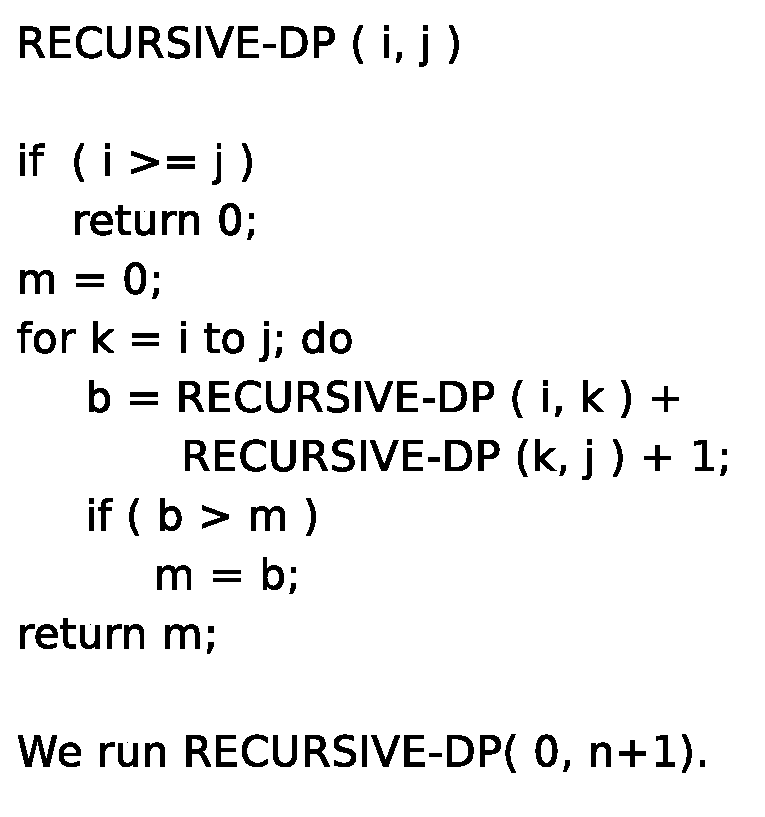
\includegraphics[width=1.0\textwidth]{L7-intervalschedulingdpalgo.eps}%
%      \end{minipage}%
%  \quad
%      \begin{minipage}{0.30\textwidth}
%       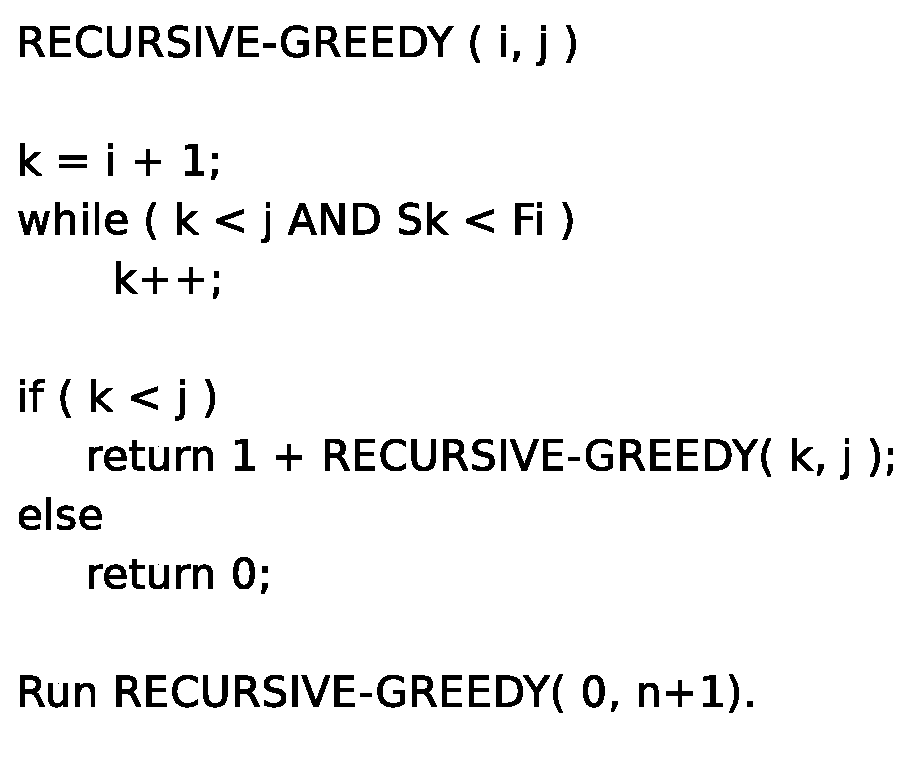
\includegraphics[width=1.0\textwidth]{L7-intervalschedulinggreedyalgo.eps}%
%      \end{minipage}%
%  \quad
%       \begin{minipage}{0.25\textwidth}
%       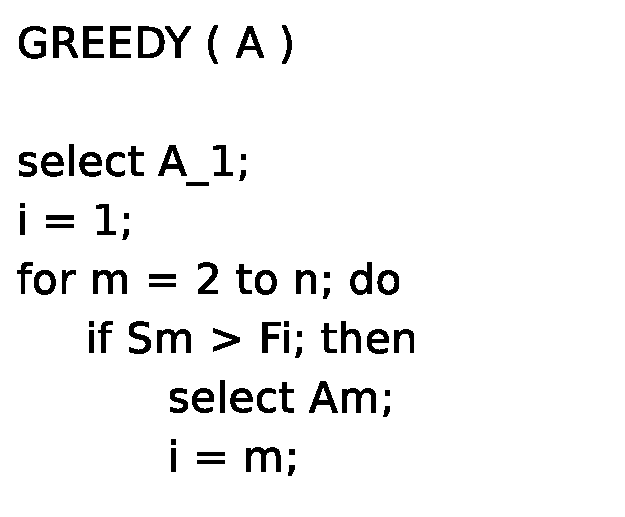
\includegraphics[width=1.0\textwidth]{L7-intervalschedulinggreedyalgo2.eps}%
%      \end{minipage}%
% 
%  \end{figure}
% 
% DP algorithm:  we have $j-i-1$ options when solving $A_{i..j}$, and a choice yields two subproblems.  \\
% Time-complexity: $O(n^3)$.       
% }
% 
% \frame[allowframebreaks]{
% \frametitle{Simplifying the dynamic programming algorithm to greedy algorithm }
% 
%  \begin{figure}%
%      \begin{minipage}{0.32\textwidth}%
%       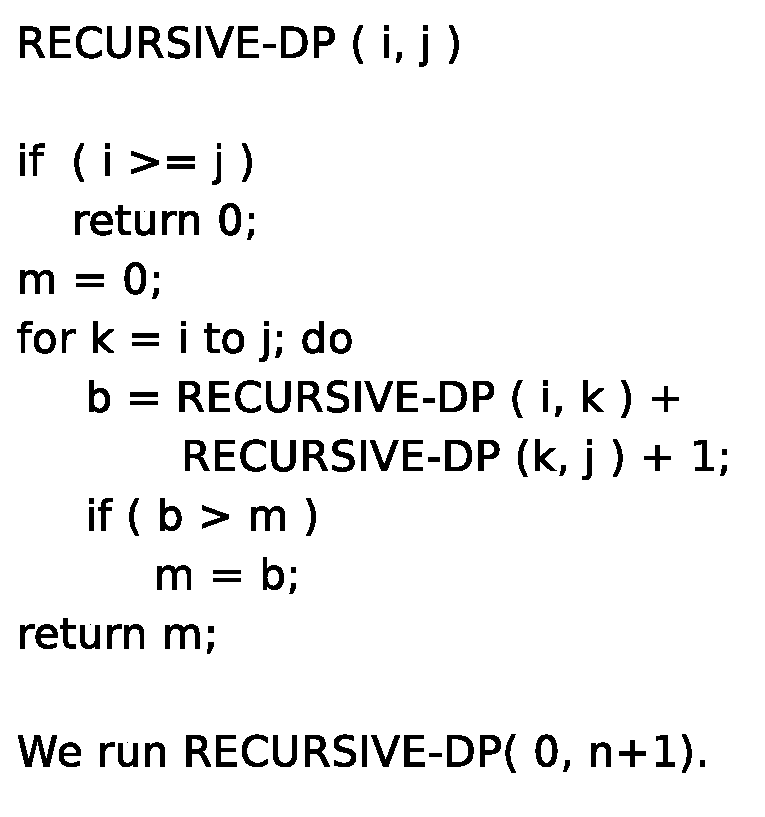
\includegraphics[width=1.0\textwidth]{L7-intervalschedulingdpalgo.eps}%
%      \end{minipage}%
%  \quad
%      \begin{minipage}{0.30\textwidth}
%       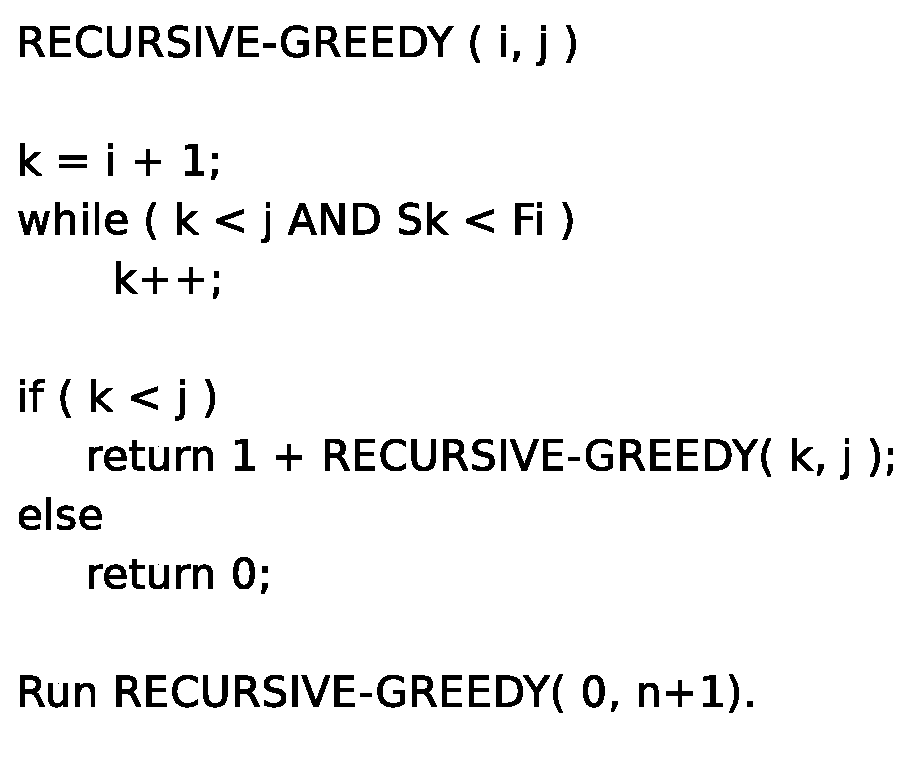
\includegraphics[width=1.0\textwidth]{L7-intervalschedulinggreedyalgo.eps}%
%      \end{minipage}%
%  \quad
%       \begin{minipage}{0.25\textwidth}
%       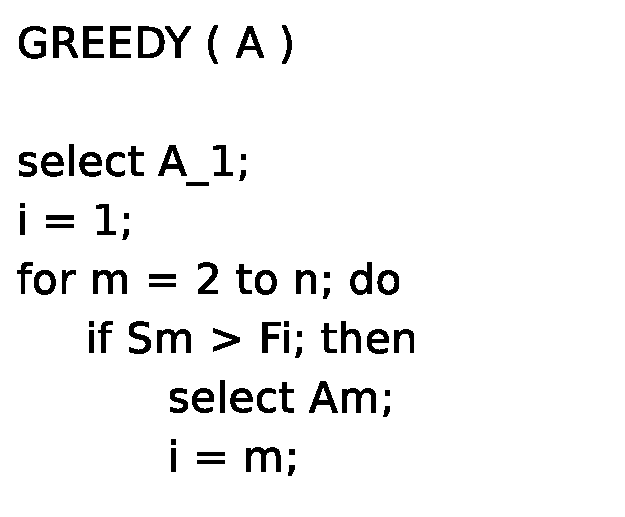
\includegraphics[width=1.0\textwidth]{L7-intervalschedulinggreedyalgo2.eps}%
%      \end{minipage}%
% 
%  \end{figure}
% 
% Greedy algorithm:  only one option (greedy-selection), and the subproblem $A_{ik}$ is empty. Thus choosing $A_k$ leads to only one subproblem. \\
% Time-complexity: $O(n \log n )$. 
% }
% 
% \frame[allowframebreaks]{
% \frametitle{Simplifying the dynamic programming algorithm to greedy algorithm }
% 
%  \begin{figure}%
%      \begin{minipage}{0.32\textwidth}%
%       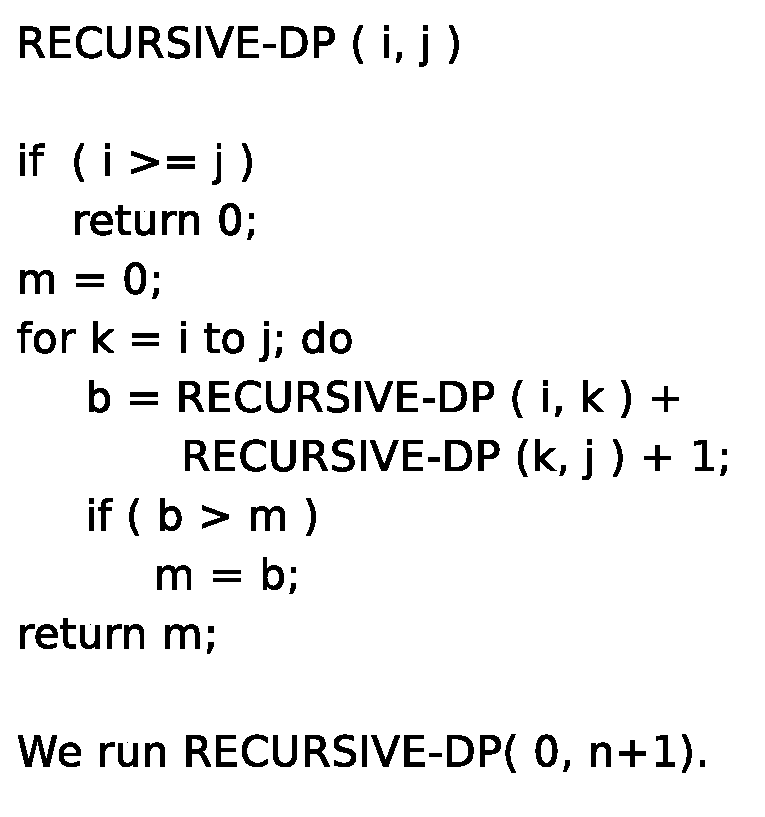
\includegraphics[width=1.0\textwidth]{L7-intervalschedulingdpalgo.eps}%
%      \end{minipage}%
%  \quad
%      \begin{minipage}{0.30\textwidth}
%       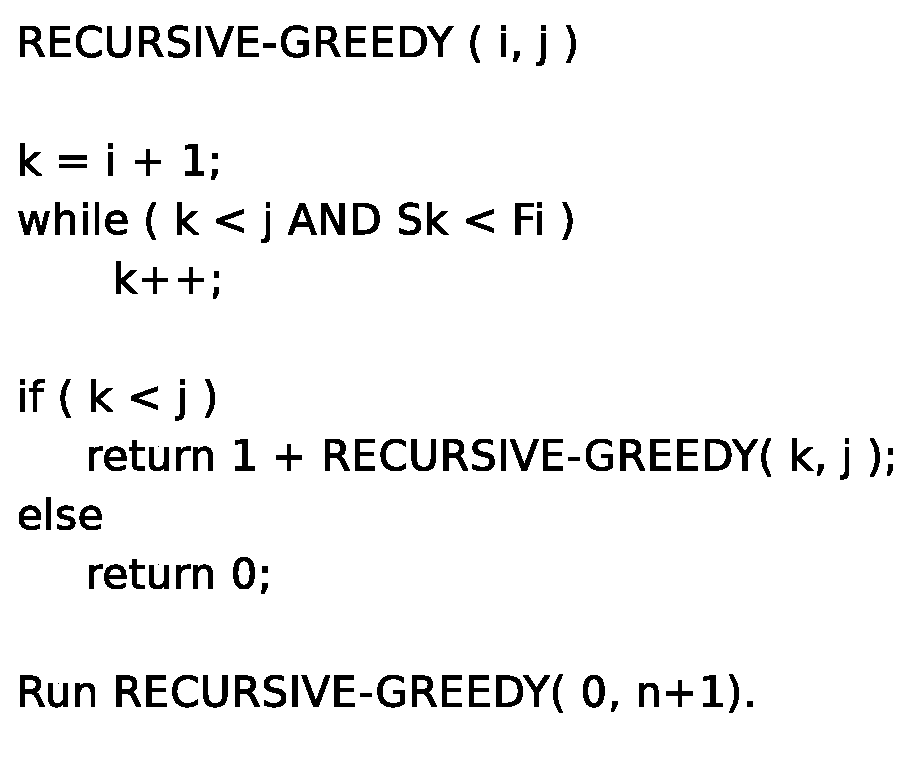
\includegraphics[width=1.0\textwidth]{L7-intervalschedulinggreedyalgo.eps}%
%      \end{minipage}%
%  \quad
%       \begin{minipage}{0.25\textwidth}
%       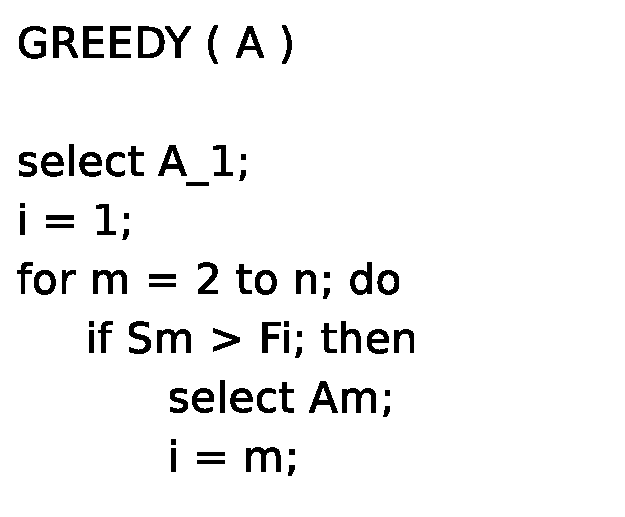
\includegraphics[width=1.0\textwidth]{L7-intervalschedulinggreedyalgo2.eps}%
%      \end{minipage}%
% \end{figure}
% We can solve each subproblem in a top-down fashion, rather than a bottom-up manner typically used in DP.  
% }

%\frame[allowframebreaks]{
%\frametitle{An example } 
%Step 1: 
%\begin{figure}
% \includegraphics[width=4.1in] {L7-intervalschedulingexamplegreedystep1.eps}
%\end{figure}
%
%Step 2: 
%\begin{figure}
% \includegraphics[width=4.1in] {L7-intervalschedulingexamplegreedystep2.eps}
%\end{figure}
%
%\ \\
%\ \\
%Step 3: 
%\begin{figure}
% \includegraphics[width=4in] {L7-intervalschedulingexamplegreedystep3.eps}
%\end{figure}
%
%Step 4: 
%\begin{figure}
% 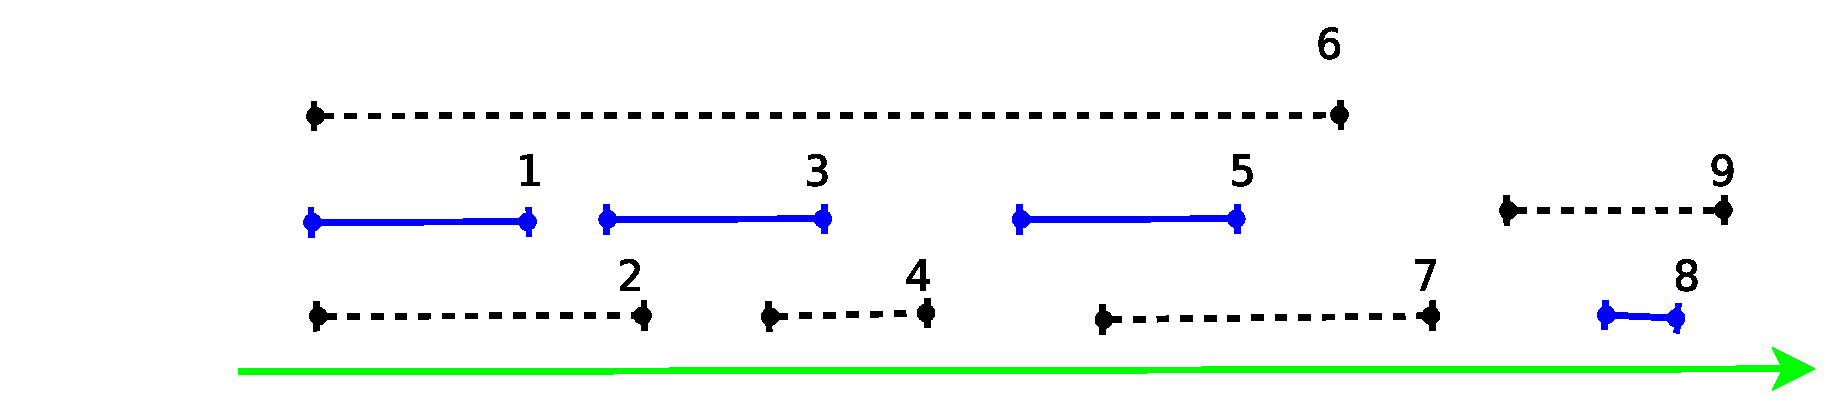
\includegraphics[width=4in] {L7-intervalschedulingexamplegreedystep4.eps}
%\end{figure}
%
%(see another demo) 
%}

\frame{
	\frametitle{An example: Step 1}


\begin{figure}[!ht]
  \centering
  \begin{tikzpicture}
  [dot/.style={circle,draw=black,fill=black,thick,inner sep=0pt,minimum size=1mm},
  bluedot/.style={circle,draw=blue,fill=blue,thick,inner sep=0pt,minimum size=1mm},
  reddot/.style={circle,draw=red,fill=red,thick,inner sep=0pt,minimum size=1mm}]
  \node[dot] (111) at (0.2,0.3) {};
  \node[dot] (112) at (2,0.3) {};
  \node[dot] (113) at (3,0.3) {};
  \node[dot] (114) at (4,0.3) {};
  \node[dot] (115) at (5,0.3) {};
  \node[dot] (116) at (7,0.3) {};
  \node[dot] (117) at (8.5,0.3) {};
  \node[dot] (118) at (9,0.3) {};
  
  \node[bluedot] (121) at (0.15,1.1) {};
  \node[bluedot] (122) at (1.3,1.1) {};
  \node[dot] (123) at (1.8,1.1) {};
  \node[dot] (124) at (3.5,1.1) {};
  \node[dot] (125) at (4.6,1.1) {};
  \node[dot] (126) at (6,1.1) {};
  \node[dot] (127) at (7.8,1.1) {};
  \node[dot] (128) at (9.4,1.1) {};
  
  \node[dot] (131) at (0.2,1.9) {};
  \node[dot] (132) at (6.5,1.9) {};
  
  \draw [dashed,black,thick] (111) -- (112) node [midway,above,draw=none] {2};
  \draw [black,thick] (113) -- (114) node [midway,above,draw=none] {4};
  \draw [black,thick] (115) -- (116) node [midway,above,draw=none] {7};
  \draw [black,thick] (117) -- (118) node [midway,above,draw=none] {8};
  
  \draw [blue,thick] (121) -- (122) node [midway,above,draw=none] {1};
  \draw [black,thick] (123) -- (124) node [midway,above,draw=none] {3};
  \draw [black,thick] (125) -- (126) node [midway,above,draw=none] {5};
  \draw [black,thick] (127) -- (128) node [midway,above,draw=none] {9};
  
  \draw [dashed,thick] (131) -- (132) node [midway,above,draw=none] {6};
  
  \draw [->,green,thick] (0,0) -- (9.5,0);
  
  \draw [blue,thick,line width=0.05cm] (1.5,0.15) -- (9.4,0.15) -- (9.4,1.7) -- (1.5,1.7) -- (1.5,0.15);
  
  \end{tikzpicture}
\end{figure}

}

\frame{
	\frametitle{Step 2}


\begin{figure}[!ht]
  \centering
  \begin{tikzpicture}
  [dot/.style={circle,draw=black,fill=black,thick,inner sep=0pt,minimum size=1mm},
  bluedot/.style={circle,draw=blue,fill=blue,thick,inner sep=0pt,minimum size=1mm},
  reddot/.style={circle,draw=red,fill=red,thick,inner sep=0pt,minimum size=1mm}]
  \node[dot] (111) at (0.2,0.3) {};
  \node[dot] (112) at (2,0.3) {};
  \node[dot] (113) at (3,0.3) {};
  \node[dot] (114) at (4,0.3) {};
  \node[dot] (115) at (5,0.3) {};
  \node[dot] (116) at (7,0.3) {};
  \node[dot] (117) at (8.5,0.3) {};
  \node[dot] (118) at (9,0.3) {};
  
  \node[bluedot] (121) at (0.15,1.1) {};
  \node[bluedot] (122) at (1.3,1.1) {};
  \node[bluedot] (123) at (1.8,1.1) {};
  \node[bluedot] (124) at (3.5,1.1) {};
  \node[dot] (125) at (4.6,1.1) {};
  \node[dot] (126) at (6,1.1) {};
  \node[dot] (127) at (7.8,1.1) {};
  \node[dot] (128) at (9.4,1.1) {};
  
  \node[dot] (131) at (0.2,1.9) {};
  \node[dot] (132) at (6.5,1.9) {};
  
  \draw [dashed,black,thick] (111) -- (112) node [midway,above,draw=none] {2};
  \draw [dashed,thick] (113) -- (114) node [midway,above,draw=none] {4};
  \draw [black,thick] (115) -- (116) node [midway,above,draw=none] {7};
  \draw [black,thick] (117) -- (118) node [midway,above,draw=none] {8};
  
  \draw [blue,thick] (121) -- (122) node [midway,above,draw=none] {1};
  \draw [blue,thick] (123) -- (124) node [midway,above,draw=none] {3};
  \draw [black,thick] (125) -- (126) node [midway,above,draw=none] {5};
  \draw [black,thick] (127) -- (128) node [midway,above,draw=none] {9};
  
  \draw [dashed,thick] (131) -- (132) node [midway,above,draw=none] {6};
  
  \draw [->,green,thick] (0,0) -- (9.5,0);
  
  \draw [blue,thick,line width=0.05cm] (4.3,0.15) -- (9.4,0.15) -- (9.4,1.7) -- (4.3,1.7) -- (4.3,0.15);
  
  \end{tikzpicture}
  %\caption{L7-intervalschedulingexamplegreedystep2.eps}
\end{figure}

}

\frame{
	\frametitle{Step 3}

\begin{figure}[!ht]
  \centering
  \begin{tikzpicture}
  [dot/.style={circle,draw=black,fill=black,thick,inner sep=0pt,minimum size=1mm},
  bluedot/.style={circle,draw=blue,fill=blue,thick,inner sep=0pt,minimum size=1mm},
  reddot/.style={circle,draw=red,fill=red,thick,inner sep=0pt,minimum size=1mm}]
  \node[dot] (111) at (0.2,0.3) {};
  \node[dot] (112) at (2,0.3) {};
  \node[dot] (113) at (3,0.3) {};
  \node[dot] (114) at (4,0.3) {};
  \node[dot] (115) at (5,0.3) {};
  \node[dot] (116) at (7,0.3) {};
  \node[dot] (117) at (8.5,0.3) {};
  \node[dot] (118) at (9,0.3) {};
  
  \node[bluedot] (121) at (0.15,1.1) {};
  \node[bluedot] (122) at (1.3,1.1) {};
  \node[bluedot] (123) at (1.8,1.1) {};
  \node[bluedot] (124) at (3.5,1.1) {};
  \node[bluedot] (125) at (4.6,1.1) {};
  \node[bluedot] (126) at (6,1.1) {};
  \node[dot] (127) at (7.8,1.1) {};
  \node[dot] (128) at (9.4,1.1) {};
  
  \node[dot] (131) at (0.2,1.9) {};
  \node[dot] (132) at (6.5,1.9) {};
  
  \draw [dashed,black,thick] (111) -- (112) node [midway,above,draw=none] {2};
  \draw [dashed,thick] (113) -- (114) node [midway,above,draw=none] {4};
  \draw [dashed,thick] (115) -- (116) node [midway,above,draw=none] {7};
  \draw [black,thick] (117) -- (118) node [midway,above,draw=none] {8};
  
  \draw [blue,thick] (121) -- (122) node [midway,above,draw=none] {1};
  \draw [blue,thick] (123) -- (124) node [midway,above,draw=none] {3};
  \draw [blue,thick] (125) -- (126) node [midway,above,draw=none] {5};
  \draw [black,thick] (127) -- (128) node [midway,above,draw=none] {9};
  
  \draw [dashed,thick] (131) -- (132) node [midway,above,draw=none] {6};
  
  \draw [->,green,thick] (0,0) -- (9.5,0);
  
  \draw [blue,thick,line width=0.05cm] (7.5,0.15) -- (9.4,0.15) -- (9.4,1.7) -- (7.5,1.7) -- (7.5,0.15);
  
  \end{tikzpicture}
\end{figure}
}

\frame{
	\frametitle{Step 4}
\begin{figure}[!ht]
  \centering
  \begin{tikzpicture}
  [dot/.style={circle,draw=black,fill=black,thick,inner sep=0pt,minimum size=1mm},
  bluedot/.style={circle,draw=blue,fill=blue,thick,inner sep=0pt,minimum size=1mm},
  reddot/.style={circle,draw=red,fill=red,thick,inner sep=0pt,minimum size=1mm}]
  \node[dot] (111) at (0.2,0.3) {};
  \node[dot] (112) at (2,0.3) {};
  \node[dot] (113) at (3,0.3) {};
  \node[dot] (114) at (4,0.3) {};
  \node[dot] (115) at (5,0.3) {};
  \node[dot] (116) at (7,0.3) {};
  \node[bluedot] (117) at (8.5,0.3) {};
  \node[bluedot] (118) at (9,0.3) {};
  
  \node[bluedot] (121) at (0.15,1.1) {};
  \node[bluedot] (122) at (1.3,1.1) {};
  \node[bluedot] (123) at (1.8,1.1) {};
  \node[bluedot] (124) at (3.5,1.1) {};
  \node[bluedot] (125) at (4.6,1.1) {};
  \node[bluedot] (126) at (6,1.1) {};
  \node[dot] (127) at (7.8,1.1) {};
  \node[dot] (128) at (9.4,1.1) {};
  
  \node[dot] (131) at (0.2,1.9) {};
  \node[dot] (132) at (6.5,1.9) {};
  
  \draw [dashed,black,thick] (111) -- (112) node [midway,above,draw=none] {2};
  \draw [dashed,thick] (113) -- (114) node [midway,above,draw=none] {4};
  \draw [dashed,thick] (115) -- (116) node [midway,above,draw=none] {7};
  \draw [blue,thick] (117) -- (118) node [midway,above,draw=none] {8};
  
  \draw [blue,thick] (121) -- (122) node [midway,above,draw=none] {1};
  \draw [blue,thick] (123) -- (124) node [midway,above,draw=none] {3};
  \draw [blue,thick] (125) -- (126) node [midway,above,draw=none] {5};
  \draw [dashed,thick] (127) -- (128) node [midway,above,draw=none] {9};
  
  \draw [dashed,thick] (131) -- (132) node [midway,above,draw=none] {6};
  
  \draw [->,green,thick] (0,0) -- (9.5,0);
  
  \end{tikzpicture}
\end{figure}
	
	
}

%\frame{
%\frametitle{Analysis  }
%
%\begin{itemize}
%\item 
%
% \item 
%  Unlike \textcolor{blue}{\bf enumerating all possible options} in DP, it suffices to use \textcolor{blue}{\bf only one option},  i.e. greedy-selection,  at each decision step. Thus, the sub-problem $A_{ik}$ is {\it null}  and only one sub-problem is left. 
%\item Notice that the greedy-selection is determined without knowledge of solutions to subproblems. 
%\end{itemize}
%}


\frame{
	\frametitle{Greedy-selection rule in multistage decision process}
\begin{figure}
\begin{tikzpicture}[scale=0.8, auto,swap]

    \def\dx{0};
   \def\dy{0.9} 
%    \foreach \pos/ \name in {{(-1.8+\dx,0+\dy)/a},{(1.8+\dx,0+\dy)/b}, {(-0.9+\dx,1.3+\dy)/e}, {(0.9+\dx,1.3+\dy)/c}, {(0+\dx,2.6+\dy)/d}}         
%    	\node[smallvertex,fill=blue!20] (\name) at \pos{$\name$};
%     
%    % Connect vertices with edges and draw weights
%     %   \foreach \source/ \dest/\weight in {a/b/{3},   c/a/{4}, e/a/{7}, a/d/{2}, b/c/{4}, b/d/{6}, e/b/{3}, c/d/{5}, c/e/{8}, d/e/{6}}
%    \foreach \source/ \dest/\weight in {a/b/{e_1{:}\ 3},   a/c/{}, e/a/{e_{5}{:}\  7}, b/c/{e_{4}{:}\  4}, b/e/{}, c/d/, c/e/{e_{9}{:}\  8}, d/e/}
%        \path[undirectededge] (\source) -- node[weight] {\tiny $\weight$} (\dest);
%         
%    \draw[thick] (a)   to [out=140, in=180] node[left] {\tiny $e_{3}{:}\  2$} (d);   
%        \draw[thick] (b)   to [out=40, in=0] node[right] {\tiny $e_{6}{:}\  6$} (d);   
%        
%       \foreach \source/ \dest/\weight in {a/b/,   b/c/,  c/d/, d/e/, e/a/}
%        \path[undirectededge] (\source) -- node[weight] {$\weight$} (\dest);
%
%   \node[] at (-0.7+\dx, 0.3+\dy) {\tiny $e_{2}{:}\  4$}; 
%   \node[] at (0.7+\dx, 0.3+\dy) {\tiny $e_{7}{:}\  3$}; 
%  \node[] at (-0.9+\dx, 2.0+\dy) {\tiny $e_{10}{:}\  6$}; 
%  \node[] at (0.9+\dx, 2.0+\dy) {\tiny $e_{8}{:}\  5$}; 
 
%Tree

	\def\d{2.4}; 
	\def\e{1.5};
	\def\f{1.0};
	\def\h{1.5};

% Label
	
   \node at ( -1.5*\d - 2*\e, -\h * 0.5)  {\tiny $x_1=A_1/A_2/.../A_9$};  

%layer 1	
    \foreach \pos/\name/\label in {{(0,0)/root/}} 
        \node[tinyvertex,draw=black, fill=white!20] (\name) at \pos {};
%layer 2	
    \foreach \pos/\name/\label in { {(-1.5*\d, -1*\h)/L11/}, {(-0.5*\d,-1*\h)/L12/}, {(1.5*\d, -1*\h)/L14/}}  
        \node[tinyvertex,draw=black, fill=white!20] (\name) at \pos {};	

            
 % Edges 
 	%layer 1
  	\foreach \source/ \dest /\weight in {root/L11/, root/L12/, root/L14/ }         
		\path[undirectededge] (\source) -- node[weight] { } (\dest);

  	\foreach \source/ \dest /\weight in {root/L11/}         
		\path[undirectededge, red, ultra thick] (\source) -- node[weight] { } (\dest);



   %Label
   \def\s{1.05};  
   \def\t{0.3};  
   \node[] at (0 + \s, 0) {\tiny $X=[??...?]$}; 
   \node[] at (0 + \s, 0 - \t) {\tiny ${\tiny P_{0}}$}; 
 
  %layer 1
    \def\s{0.75};  
   \node[] at (-1.5*\d + \s, -1*\h-\t ) {\tiny $X=[A_1?...?]$}; 
   \node[] at (-1.5*\d + \s, -1*\h-\t  - \t) {\tiny ${\tiny P_{1}}$ }; 

   \node[] at (-0.5*\d + \s, -1*\h-\t ) {\tiny $X=[A_2?...?]$}; 
   \node[] at (-0.5*\d + \s, -1*\h-\t  - \t) {\tiny ${\tiny P_{2}}$ }; 
  
  \node[] at (0.5*\d + \s, -1*\h-\t ) {......};
  
%   \node[] at (0.5*\d + \s, -1*\h-\t ) {\tiny $A_8$?...?}; 
%   \node[] at (0.5*\d + \s, -1*\h-\t  - \t) {\tiny ${\tiny P_{8}}$ }; 

   \node[] at (1.5*\d + \s, -1*\h-\t ) {\tiny $X=[A_9?...?]$  }; 
   \node[] at (1.5*\d + \s, -1*\h-\t  - \t) {\tiny ${\tiny P_{9}}$ }; 

   \end{tikzpicture}
\end{figure}

\begin{itemize}
	\item Here we represent the optimal solution as $X=[x_1, x_2, ......]$, where $x_i\in \{A_1, A_2, ..., A_9\}$ denotes the activity selected at the $i$-th decision step. 
	\item At the first decision step, the dynamic programming technique has to enumerate 9 options $x_1 = A_1$, $x_1 = A_2$, ..., $x_1 = A_9$ as it is unknown which one is optimal, i.e., 
\[
OPT(S) = \max_{A_i \in S}\{OPT( R(S, A_i) ) + 1\}
\]
\item 	
	In contrast,  the greedy algorithm selects $A_1$ directly according to the greedy-selection property, i.e., 
\[
OPT(S) = OPT( R(S, A_1) ) + 1.
\]
	
\end{itemize}

}


\frame{
	\frametitle{Elements of greedy algorithm}
	\begin{itemize}
		\item In general, greedy algorithms have five components: 
			\begin{enumerate}
\item 			A candidate set, from which a solution is created
\item A selection function, which chooses the best candidate to be added to the solution
\item A feasibility function, that is used to determine if a candidate can be used to contribute to a solution
\item An objective function, which assigns a value to a solution, or a partial solution, and
\item A solution function, which will indicate when we have discovered a complete solution
			\end{enumerate}
	\end{itemize}

}

\frame{
\frametitle{DP versus Greedy }
Similarities: 
\begin{enumerate}
\item
Both dynamic programming and greedy techniques are typically applied to \textcolor{red}{\bf optimization} problems. 
\item \textcolor{red}{\bf Optimal substructure}: Both dynamic programming and greedy techniques exploit the optimal substructure property. 
\item \textcolor{blue}{ {\bf Beneath every greedy algorithm, there is almost always a more cumbersome dynamic programming solution \quad --- CRLS} }
\end{enumerate}

} 

\frame{
\frametitle{DP versus Greedy  cont'd}

Differences: 
\begin{enumerate}
 \item A dynamic programming method typically \textcolor{red}{\bf enumerate all possible options at a decision step}, and the decision cannot be determined before subproblems were solved.
 \item In contrast, greedy algorithm does not need to enumerate all possible options---it simply \textcolor{red}{\bf make a locally optimal (greedy) decision} without considering results of subproblems. 
\end{enumerate}
Note: 
\begin{itemize}
	\item Here, ``\textcolor{red}{local}'' means that we have already acquired part of an optimal solution, and the partial knowledge of optimal solution is sufficient to help us make a wise decision. 
	\item Sometimes a rigorous proof is unavailable, thus extensive experimental results are needed to show the efficiency of the greedy technique. 
\end{itemize}

}

\frame{
\frametitle{How to design greedy method?} 
Two strategies:
\begin{enumerate}
 \item Simplifying a dynamic programming method through greedy-selection;
 \item Trial-and-error: Describing the solution-generating process as making a sequence of choices, and trying different greedy-selection rules.
\end{enumerate}


}

\frame{
	\begin{block}{}
		Trying other greedy rules 
	\end{block} 
}

\frame{
\frametitle{Incorrect trial 1: {\bf earlist start} rule } 
\begin{itemize}
\item Intuition: the earlier start time, the better.   
\item Incorrect. A negative example: 
%\begin{figure}
% 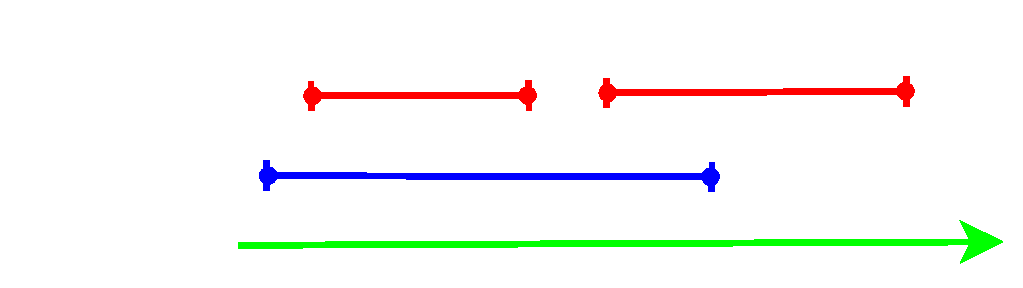
\includegraphics[width=2in] {L7-intervalschedulingexample-error2.eps}
%\end{figure}

\begin{figure}[!ht]
  \centering
  \begin{tikzpicture}
  [dot/.style={circle,draw=black,fill=black,thick,inner sep=0pt,minimum size=1mm},
  bluedot/.style={circle,draw=blue,fill=blue,thick,inner sep=0pt,minimum size=1mm},
  reddot/.style={circle,draw=red,fill=red,thick,inner sep=0pt,minimum size=1mm}]
  \node[bluedot] (111) at (0.2,0.3) {};
  \node[bluedot] (112) at (3,0.3) {};
  
  \node[reddot] (121) at (0.4,1.1) {};
  \node[reddot] (122) at (1.8,1.1) {};
  \node[reddot] (123) at (2.3,1.1) {};
  \node[reddot] (124) at (4,1.1) {};
  
  \draw [blue,thick] (111) -- (112);
  
  \draw [red,thick] (121) -- (122);
  \draw [red,thick] (123) -- (124);
  
  \draw [->,green,thick] (0,0) -- (5,0);
  
  \end{tikzpicture}
%  \caption{L7-intervalschedulingexample-error2.eps}
\end{figure}



 \item 
Greedy solution: blue one. Solution value: 1. 
\item 
Optimal solution: red ones. Solution value: 2.
\end{itemize}
}

\frame{
\frametitle{Incorrect trial 2: trying {\bf minimal duration } rule } 
\begin{itemize}
\item Intuition: the shorter duration, the better. 
\item Incorrect. A negative example: 

\begin{figure}[!ht]
  \centering
  \begin{tikzpicture}
  [dot/.style={circle,draw=black,fill=black,thick,inner sep=0pt,minimum size=1mm},
  bluedot/.style={circle,draw=blue,fill=blue,thick,inner sep=0pt,minimum size=1mm},
  reddot/.style={circle,draw=red,fill=red,thick,inner sep=0pt,minimum size=1mm}]
  \node[bluedot] (111) at (1.5,0.3) {};
  \node[bluedot] (112) at (2.8,0.3) {};
  
  \node[reddot] (121) at (0.4,1.1) {};
  \node[reddot] (122) at (1.8,1.1) {};
  \node[reddot] (123) at (2.3,1.1) {};
  \node[reddot] (124) at (4,1.1) {};
  
  \draw [blue,thick] (111) -- (112);
  
  \draw [red,thick] (121) -- (122);
  \draw [red,thick] (123) -- (124);
  
  \draw [->,green,thick] (0,0) -- (5,0);
  
  \end{tikzpicture}
%  \caption{L7-intervalschedulingexample-error1.eps}
\end{figure}

 \item 
Greedy solution: blue one. Solution value: 1. 
\item 
Optimal solution: red ones. Solution value: 2.
\end{itemize}
}


\frame{
\frametitle{Incorrect trial 3: trying {\bf minimal conflicts } rule } 
\begin{itemize}
\item Intuition: the less conflict activities, the better. 
\item Incorrect. A negative example: 
%\begin{figure}
% 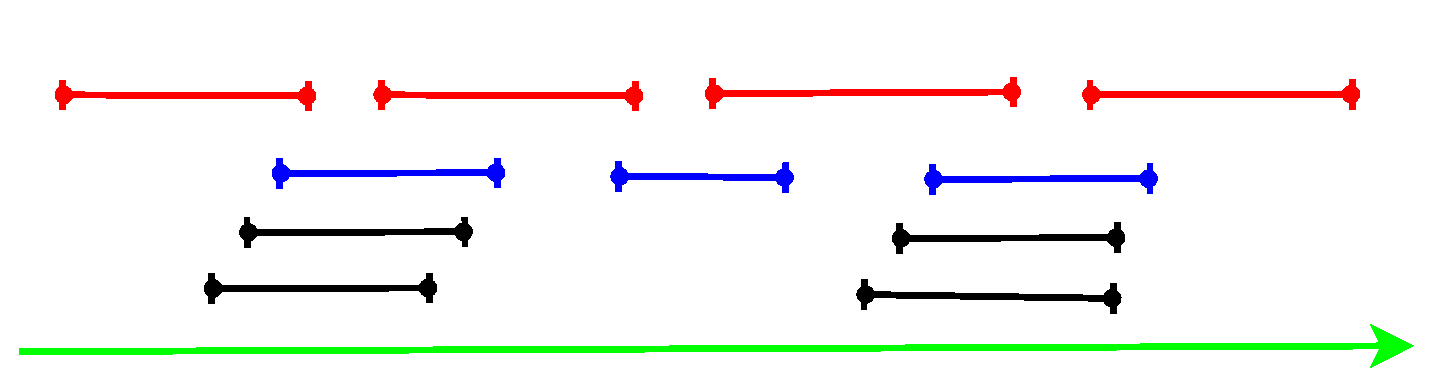
\includegraphics[width=3in] {L7-intervalschedulingexample-error3.eps}
%\end{figure}


\begin{figure}[!ht]
  \centering
  \begin{tikzpicture}
  [dot/.style={circle,draw=black,fill=black,thick,inner sep=0pt,minimum size=1mm},
  bluedot/.style={circle,draw=blue,fill=blue,thick,inner sep=0pt,minimum size=1mm},
  reddot/.style={circle,draw=red,fill=red,thick,inner sep=0pt,minimum size=1mm}]
  \node[dot] (111) at (1.5,0.3) {};
  \node[dot] (112) at (2.8,0.3) {};
  \node[dot] (113) at (5.5,0.3) {};
  \node[dot] (114) at (7.2,0.3) {};
  
  \node[dot] (121) at (1.7,0.8) {};
  \node[dot] (122) at (3,.8) {};
  \node[dot] (123) at (5.7,.8) {};
  \node[dot] (124) at (7.2,.8) {};
  
  \node[bluedot] (131) at (1.9,1.3) {};
  \node[bluedot] (132) at (3.2,1.3) {};
  \node[bluedot] (133) at (4,1.3) {};
  \node[bluedot] (134) at (5,1.3) {};
  \node[bluedot] (135) at (5.9,1.3) {};
  \node[bluedot] (136) at (7.4,1.3) {};
  
  \node[reddot] (141) at (0.3,1.8) {};
  \node[reddot] (142) at (2.3,1.8) {};
  \node[reddot] (143) at (2.7,1.8) {};
  \node[reddot] (144) at (4.1,1.8) {};
  \node[reddot] (145) at (4.5,1.8) {};
  \node[reddot] (146) at (6.5,1.8) {};
  \node[reddot] (147) at (7,1.8) {};
  \node[reddot] (148) at (9,1.8) {};
  
  \draw [black,thick] (111) -- (112);
  \draw [black,thick] (113) -- (114);
  
  \draw [black,thick] (121) -- (122);
  \draw [black,thick] (123) -- (124);
  
  \draw [blue,thick] (131) -- (132);
  \draw [blue,thick] (133) -- (134);
  \draw [blue,thick] (135) -- (136);
  
  \draw [red,thick] (141) -- (142);
  \draw [red,thick] (143) -- (144);
  \draw [red,thick] (145) -- (146);
  \draw [red,thick] (147) -- (148);
  
  \draw [->,green,thick] (0,0) -- (9.55,0);
  
  \end{tikzpicture}
\end{figure}


 \item 
Greedy solution: blue ones. Solution value: 3. 
\item 
Optimal solution: red ones. Solution value: 4.
\end{itemize}
}
%
%\frame[allowframebreaks]{
%\frametitle{Elements of greedy strategy}
%
%Greedy choice: 
%\begin{enumerate}
% \item 
%Describing the solving process as making a sequence of choices. 
%\item At each decision point, the choice that \textcolor{red}{\bf seems best at the moment} is chosen \textcolor{red}{\bf without considering solutions to subproblems}. 
%\item Prove the greedy property, i.e.  a \textcolor{red}{\bf globally} optimal solution can be obtained through making a sequence of \textcolor{red}{\bf locally} optimal choices. 
%\end{enumerate}
%
%\begin{figure} 
%  \includegraphics[width=2.5in]{L5-incremental-dc1.png}
%\end{figure}
%} 

%\frame{
%\frametitle{Properties of problems that greedy strategy can apply}
%
%\begin{enumerate}
% \item Divide-and-conquer: problem can be reduced into \textcolor{red}{\bf smaller, independent subproblems}; 
%
% \item {\bf Optimal substructure property}: an \textcolor{red}{\bf optimal solution} to the problem contains within it \textcolor{red}{optimal solutions} to subproblems. Thus we have a recursive solution as results. 
%
%\item {\bf Greedy-selection property}: prove that at any stage, one of the locally-optimal choices can be used to construct the globally-optimal solution. 
%% 
%% \item top-down fashion: show that all but one subproblems induced by having made the greedy choice are empty. 
%\end{enumerate}
%}

%\frame{
%\begin{block}{}
% Revisiting {\sc Knapsack} problem
%\end{block}
%}

%\frame[allowframebreaks]{
%\frametitle{{\sc Knapsack} problem}
%\begin{block}{}
%\begin{itemize}
%    \item {\bf Input:}\\ $n$ items. Item $i$ has weight $w_i$ and value $v_i$, and a total weight limit $W$; 
%	\item {\bf Output:}\\ A set of items to maximize the total value with total weight below $W$.
%\end{itemize}
% %\begin{itemize}
% %\item {\bf Input:} \\a set of items $i$ with weight $w$_$i$ and value $v$_$i$, and a total weight limit $W$, $i$=1,2,\cdots,$n$
% %\item {\bf Output:}\\the set of items which maximize the total value with total weight below $W$
% %\end{itemize}
%\end{block}
%Two versions of {\sc Knapsack } problem: 
%\begin{itemize}
% \item 
%{\sc 0-1 Knapsack}: each item, say gold ingot,  must be either taken or abandoned ;  \\
% \item
%{\sc Fractional Knapsack}: can take fractions of items, say gold dust. \\
%\end{itemize}
%	\begin{figure}
%	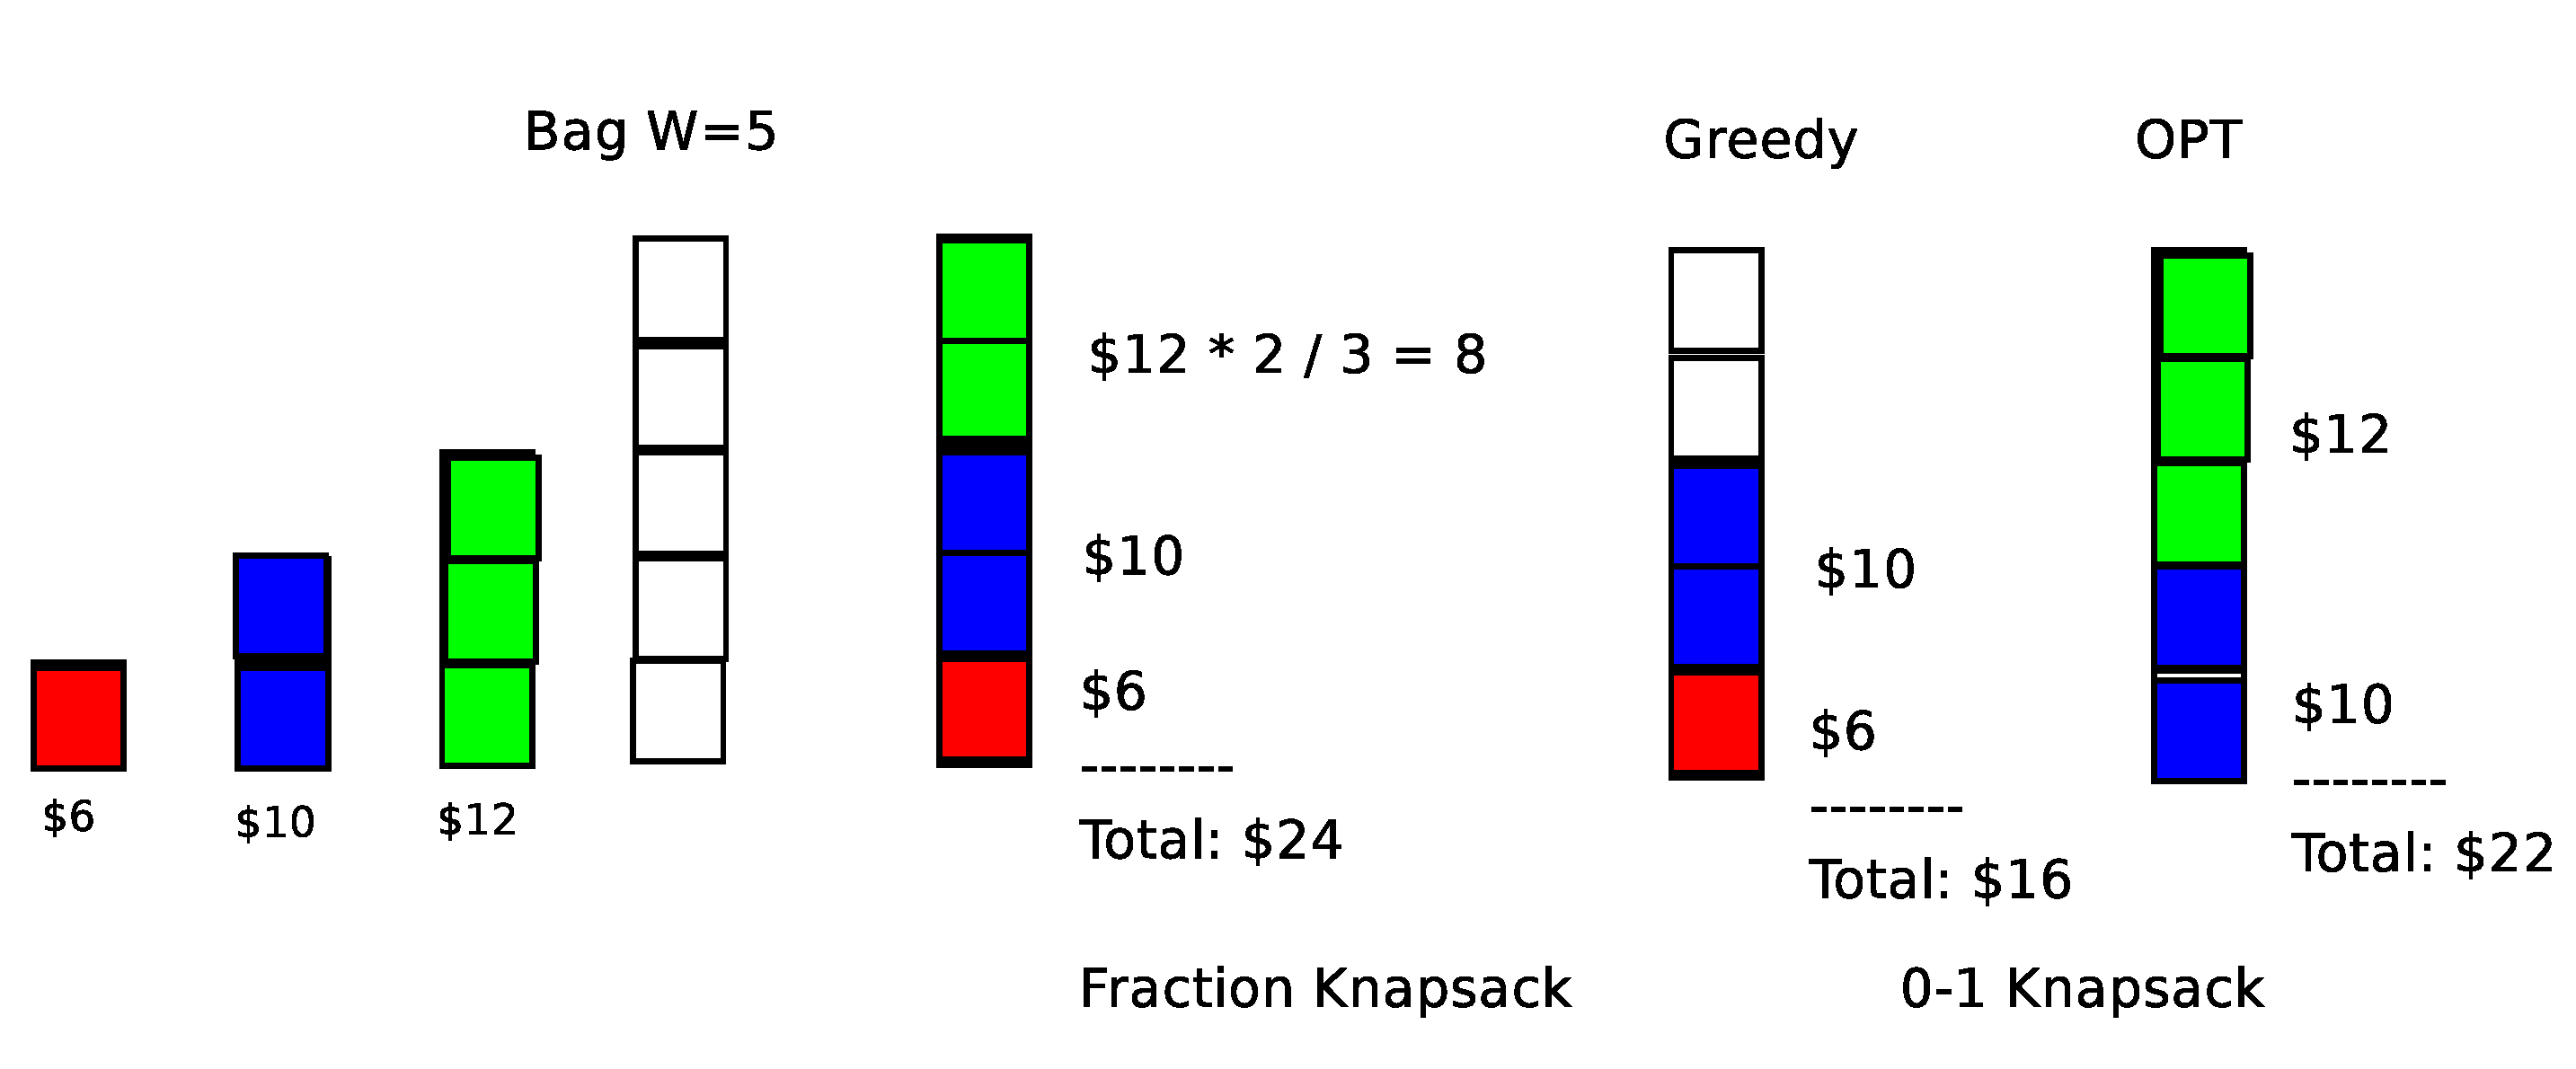
\includegraphics[width=3.5in]{L7-Knapsackexample.eps}
%	\end{figure}
%
%\begin{enumerate}
% \item Optimal substructure: both problems display the optimal substructure property; 
% \item Greedy choice property: however, the greedy choice property doesn't hold in the case of {\sc 0-1 Knapsack}--- the greedy choice of item 1 leads to a suboptimal solution. 
%\end{enumerate}
%}

\frame{
\begin{block}{}
 Revisiting {\sc ShortestPath} problem
\end{block}
%\footnote{Some pictures were excerpted from {\it Introduction to algorithms} }
}

\frame{
\frametitle{Revisiting {\sc Single Source Shortest Paths} problem }

\begin{block}{}
 {\bf INPUT: } \\ 
A directed graph $G=<V, E>$. Each edge $e=<i, j>$ has a distance  $d_{i,j}$. A single source node $s$, and a destination node $t$; \\
 {\bf OUTPUT: } \\ 
The shortest path from $s$ to $t$ (Or the shortest paths from $s$ to each node $v\in V$, or the shortest paths  from each node $v \in V$ to $t$).  \\
\end{block}

Two versions of {\sc ShortestPath} problem: \\
\begin{enumerate}
 \item No negative cycle: Bellman-Ford dynamic programming algorithm;
 \item No negative edge: Dijkstra greedy algorithm.
\end{enumerate}

% \begin{figure}
% 	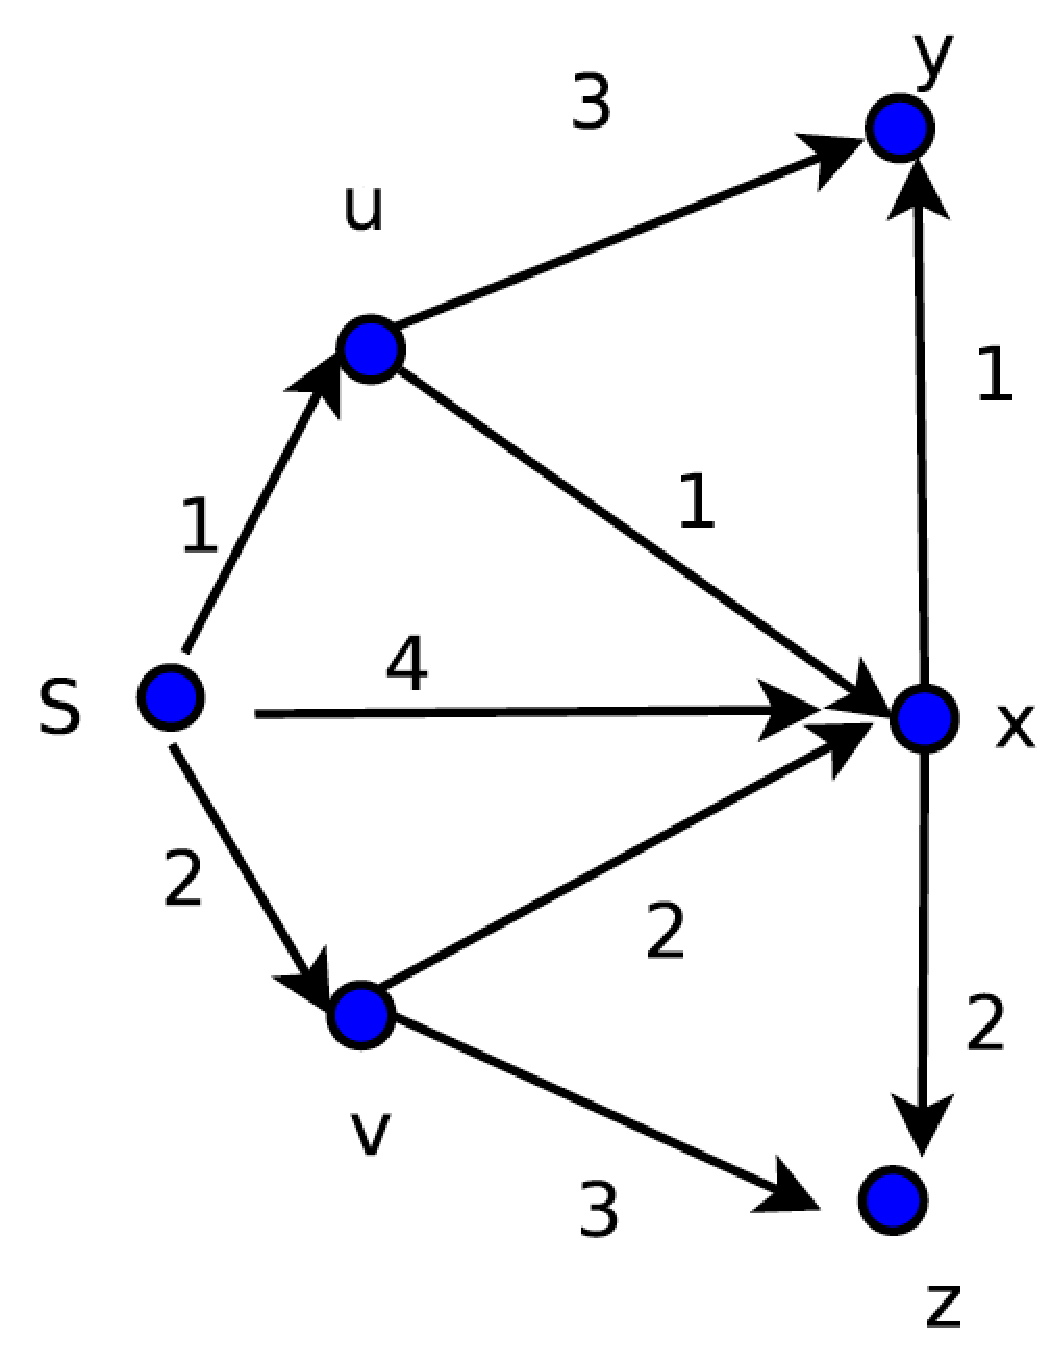
\includegraphics[width=2in]{L7-shortestpathexample.eps}
% \end{figure}
}


\frame{
	\begin{block}{}
	Optimal sub-structure property in version 1 
	\end{block} 
}

\frame{
\frametitle{Optimal sub-structure property }
\begin{itemize}
 \item Solution: a path from $s$ to $t$ with at most $(n-1)$ edges. Describing the solving process as a multi-stage decision process: at each decision step, we decide the subsequent node. 
 \item Consider the final decision (i.e. from which we reach node $t$). There are several possibilities for the decision: 
  \begin{itemize}
   \item node $v$ such that $<v,t>\in E$: then it suffices to solve a smaller subproblem, i.e.  ``starting from $s$ to node $v$ via at most $(n-2)$ edges''. 
  \end{itemize}
 \item Thus we can design the general form of sub-problems as \textcolor{red}{\bf ``starting from $s$ to a node $v$ via at most $k$ edges''}. Denote the optimal solution value as $OPT(v, k)$. 
 \item Optimal substructure: 
\begin{footnotesize}
 $OPT(v, k) = \min \begin{cases} 
                      OPT( v, k-1 ) \\
                      \textcolor{blue}{\min_{<u,v>\in E}} \{ OPT( u, k-1) + d_{u, v}  \} \\
                     \end{cases}  $
\end{footnotesize}
\item Note: the first item $OPT(v, k-1)$ is introduced here to describe \textcolor{red}{\bf ``at most''}. 
\item Time complexity: $O(mn)$
\end{itemize}
} 


\frame{
\frametitle{{\sc Bellman\_Ford} algorithm [1956] }

{\sc Bellman\_Ford}$( G, s, t )$
\begin{algorithmic}[1]
\FOR{$i=0$ to $n$ }
	\STATE $OPT[s, i] = 0;$
\ENDFOR
\FORALL{node $v \in V$ }
	\STATE $OPT[v, 0] = \infty;$
\ENDFOR 
\FOR{$k=1$ to $n-1$ }
	\FORALL{node $v$ (in an arbitrary order) }
		\STATE \begin{small} $OPT[v, k] = \min \begin{cases}
			OPT[v, k-1], \\
			\min_{<u,v>\in E} \{OPT[ u, k-1 ] + d(u,v) \} 
		\end{cases}$
		\end{small}
	\ENDFOR
\ENDFOR
\RETURN{$OPT[ t, n-1]$};
\end{algorithmic}
}

\frame{
	\frametitle{An example: Step 1}
	
\begin{figure}
% \begin{minipage}{0.40\textwidth}
%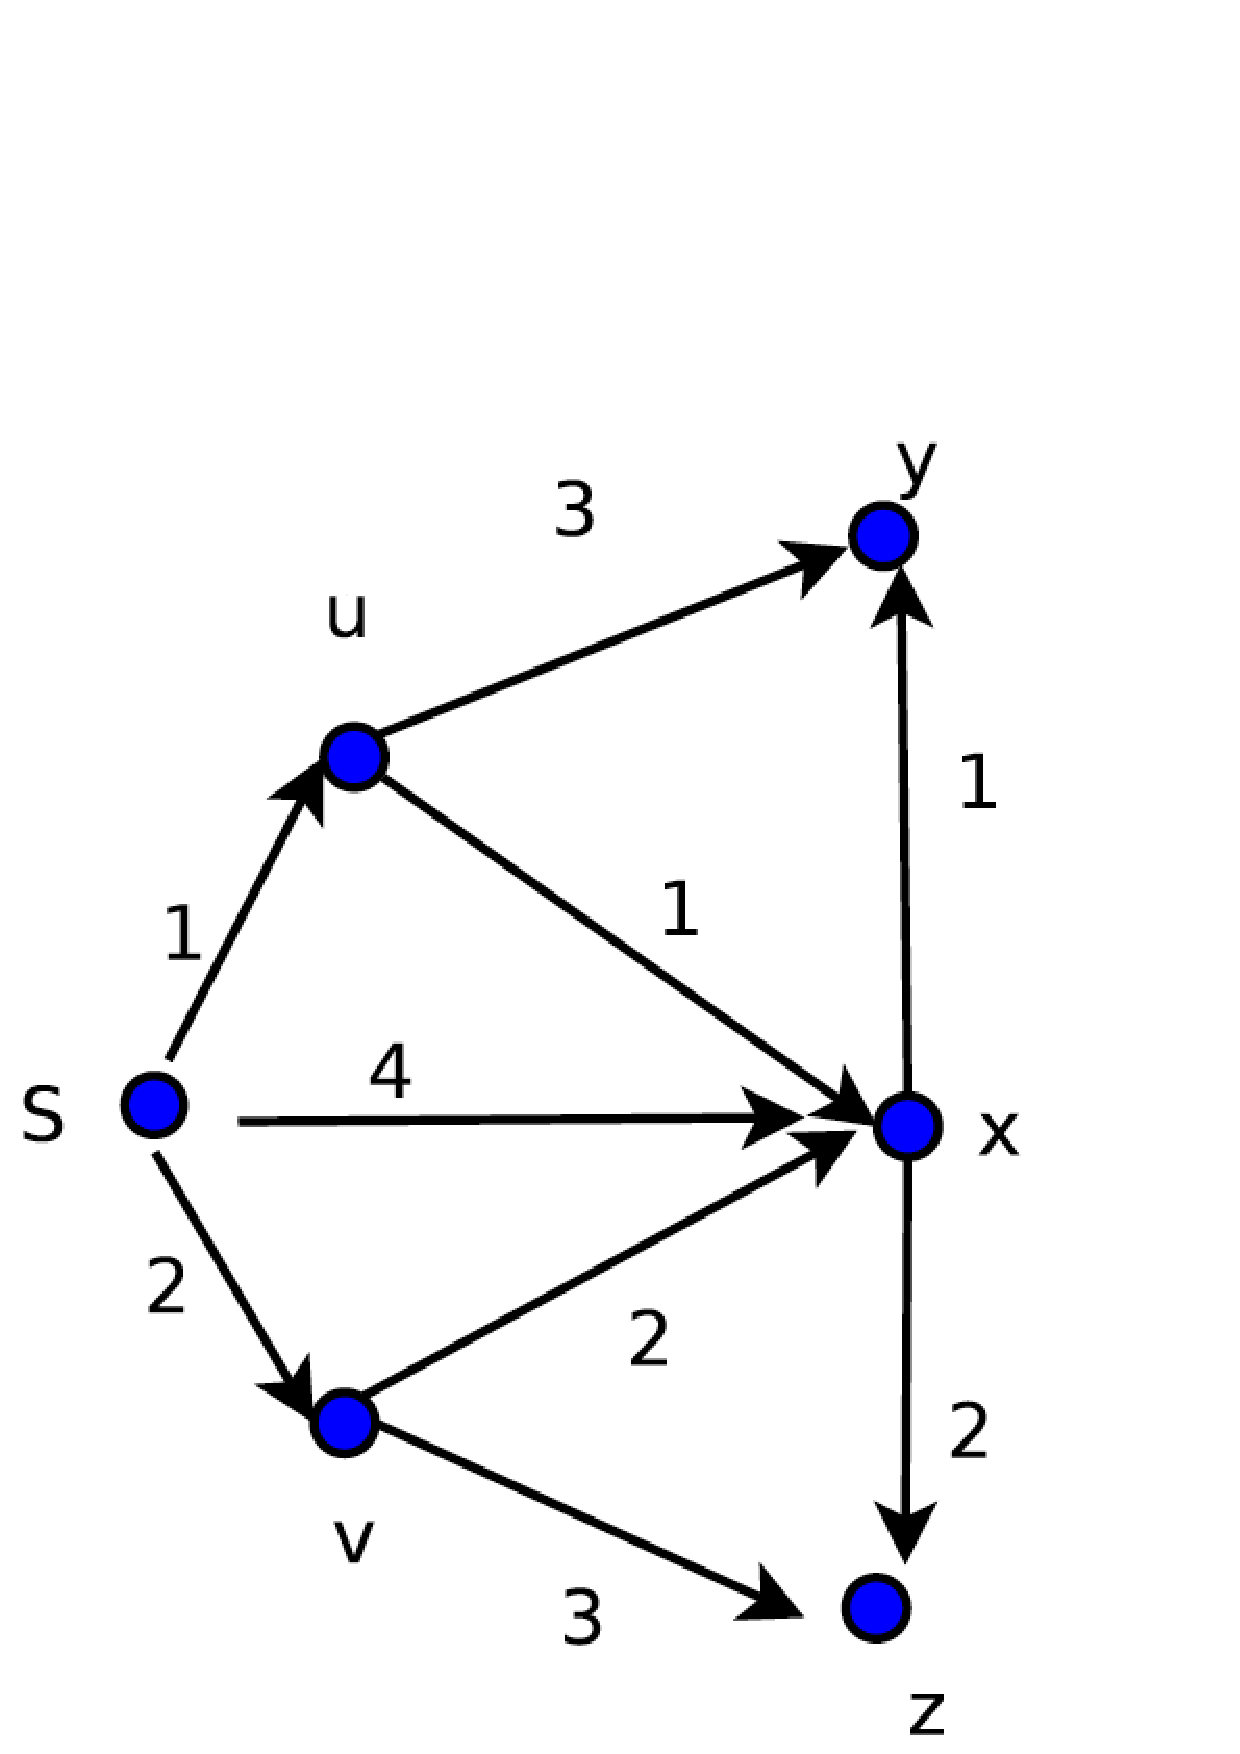
\includegraphics[width=0.9\textwidth]{L7-shortestpathexample.png}
 
\begin{tikzpicture}[auto,swap,scale=0.75]
% 
%    \foreach \pos/\name in {{(0,0)/s}, {(2,2)/u}, {(2,-2)/v}, {(5,0)/x}, {(5,-3)/z}, {(5,3)/y}}
%        \node[vertex,fill=blue!20] (\name) at \pos {$\name$};
%        
%        
%    \foreach \source/\dest/\weight in {s/u/1, s/v/2, s/x/4,   u/y/3,  u/x/1, x/y/1, v/x/2, v/z/3, x/z/2 } 
%            \path[edge] (\source) -- node[weight] {\tiny $\weight$} (\dest);
%	
%\end{tikzpicture} 
%		

  	\def\dx{-6};
 	\def\dy{-1.25};	
    \foreach \pos/\name in {{(0+\dx,0+\dy)/s}, {(2+\dx,1.4+\dy)/u}, {(2+\dx,-1.4+\dy)/v}, {(4+\dx,0+\dy)/x}, {(4+\dx,-2.5+\dy)/t}, {(4+\dx,2.5+\dy)/y}}
        \node[middlevertex,fill=blue!20] (\name) at \pos {$\name$};
        
        
    \foreach \source/\dest/\weight in {s/u/1, s/v/2, s/x/4,   u/y/3,  u/x/1, x/y/1, v/x/2, v/t/3, x/t/2 } 
            \path[edge] (\source) -- node[weight] {\tiny $\weight$} (\dest);
	
 
% \end{minipage}
% \begin{minipage}{0.45\textwidth}

%  \includegraphics[width=\textwidth]{L7-Dijkstraexample.png}
 
 %\begin{tikzpicture}[scale=0.8, auto,swap]
  
  	\def\d{0.7};
	
	%draw index 
 \def\dy{1};
 \def\dx{0};

    \foreach \i/\num/\name in { 1/k=0/, 2/1/s1,3/2/s2,4/3/s3,5/4/s4,6/5/}{
           \node[blue,thick] (\name) at (\i*\d+\d/2 + \dx*\d - \d, \d/2 + \dy * \d) {\tt \num};
    }

 \def\dy{0};
 \def\dx{0};
    \foreach \i/\num/\name in { 1/s/s1,2/u/s2,3/v/s3,4/x/s4, 5/y/,6/t/}{
         \node[blue,thick] (\name) at ( -1*\d+\d/2,  0.0 - \i*\d + \d/2 - \dy * \d + \d){$\num$};
    }

    
%score	
 \def\dy{0};
 \def\dx{0};
    \foreach \i/\num/\name in { 0/0/,1/0/S1,2/0/S2,3/0/,4/0/,5/0/}{
             \draw[  thick ] (\i*\d + \dx*\d,  0+ \dy*\d) rectangle (\i*\d+\d + \dx*\d, \d + \dy*\d);
         \node (\name) at (\i*\d+\d/2 + \dx*\d, \d/2 + \dy*\d) {\tiny $\num$};
    }



%   \draw[blue,ultra thick] (S1) circle[radius=\d/2];
%   \draw[blue,ultra thick] (S2) circle[radius=\d/2];
%   \draw[blue,ultra thick] (L) circle[radius=\d/2];
%
    
       
 \def\dy{-1};
 \def\dx{0};
    \foreach \i/\num/\name in { 0/-/,1/1/S1,2//,3//S3,4//,5//}{
             \draw[  thick ] (\i*\d + \dx*\d,  0+ \dy*\d) rectangle (\i*\d+\d + \dx*\d, \d + \dy*\d);
         \node (\name) at (\i*\d+\d/2 + \dx*\d, \d/2 + \dy*\d) {\tiny $\num$};
    }
 
%      \draw[red,ultra thick] (S1) circle[radius=\d/2];
   
    
 \def\dy{-2};
 \def\dx{0};
    \foreach \i/\num/\name in { 0/-/,1/2/,2//S1,3//S3,4//,5//}{
             \draw[  thick ] (\i*\d + \dx*\d,  0+ \dy*\d) rectangle (\i*\d+\d + \dx*\d, \d + \dy*\d);
         \node (\name) at (\i*\d+\d/2 + \dx*\d, \d/2 + \dy*\d) {\tiny $\num$};
    }
%       \draw[red,ultra thick] (S1) circle[radius=\d/2];
 
    
  \def\dy{-3};
 \def\dx{0};
    \foreach \i/\num/\name in { 0/-/,1/4/,2//S1,3//S3,4//,5//}{
             \draw[  thick ] (\i*\d + \dx*\d,  0+ \dy*\d) rectangle (\i*\d+\d + \dx*\d, \d + \dy*\d);
         \node (\name) at (\i*\d+\d/2 + \dx*\d, \d/2 + \dy*\d) {\tiny $\num$};
    }
%       \draw[red,ultra thick] (S1) circle[radius=\d/2];
  
  \def\dy{-4};
 \def\dx{0};
    \foreach \i/\num/\name in { 0/-/,1/-/,2//,3//S1,4//,5//}{
             \draw[  thick ] (\i*\d + \dx*\d,  0+ \dy*\d) rectangle (\i*\d+\d + \dx*\d, \d + \dy*\d);
         \node (\name) at (\i*\d+\d/2 + \dx*\d, \d/2 + \dy*\d) {\tiny $\num$};
    }
%         \draw[red,ultra thick] (S1) circle[radius=\d/2];

  \def\dy{-5};
 \def\dx{0};
    \foreach \i/\num/\name in { 0/-/,1/-/,2//,3//S3,4//S1,5//}{
             \draw[  thick ] (\i*\d + \dx*\d,  0+ \dy*\d) rectangle (\i*\d+\d + \dx*\d, \d + \dy*\d);
         \node (\name) at (\i*\d+\d/2 + \dx*\d, \d/2 + \dy*\d) {\tiny $\num$};
    }
%        \draw[red,ultra thick] (S1) circle[radius=\d/2];
 


%draw blue rectangles 

% \def\dy{-1};
% \def\dx{0};
%    \foreach \i/\num/\name in { 2/1/,3/1/S3,4/1/,5/1/}{
%             \draw[  thick, green ] (\i*\d + \dx*\d,  0+ \dy*\d) rectangle (\i*\d+\d + \dx*\d, \d + \dy*\d);
%    }
% 
     
    
% \def\dy{-2};
% \def\dx{0};
%    \foreach \i/\num/\name in { 3/2/S3,4/2/,5/2/}{
%             \draw[  thick, green  ] (\i*\d + \dx*\d,  0+ \dy*\d) rectangle (\i*\d+\d + \dx*\d, \d + \dy*\d);
%      }
% 
%    
%  \def\dy{-3};
% \def\dx{0};
%    \foreach \i/\num/\name in { 3/2/S3,4/2/,5/2/}{
%             \draw[  thick, green ] (\i*\d + \dx*\d,  0+ \dy*\d) rectangle (\i*\d+\d + \dx*\d, \d + \dy*\d);
%    }
% 
%   \def\dy{-4};
% \def\dx{0};
%    \foreach \i/\num/\name in { 4/3/,5/3/}{
%             \draw[  thick, green ] (\i*\d + \dx*\d,  0+ \dy*\d) rectangle (\i*\d+\d + \dx*\d, \d + \dy*\d);
%    }
% 
%  \def\dy{-5};
% \def\dx{0};
%    \foreach \i/\num/\name in {5/4/}{
%             \draw[  thick, green ] (\i*\d + \dx*\d,  0+ \dy*\d) rectangle (\i*\d+\d + \dx*\d, \d + \dy*\d);
%     }

\end{tikzpicture} 
 
% \end{minipage}
\end{figure}

	
}

\frame{
	\frametitle{Step 2}

\begin{figure}
% \begin{minipage}{0.40\textwidth}
%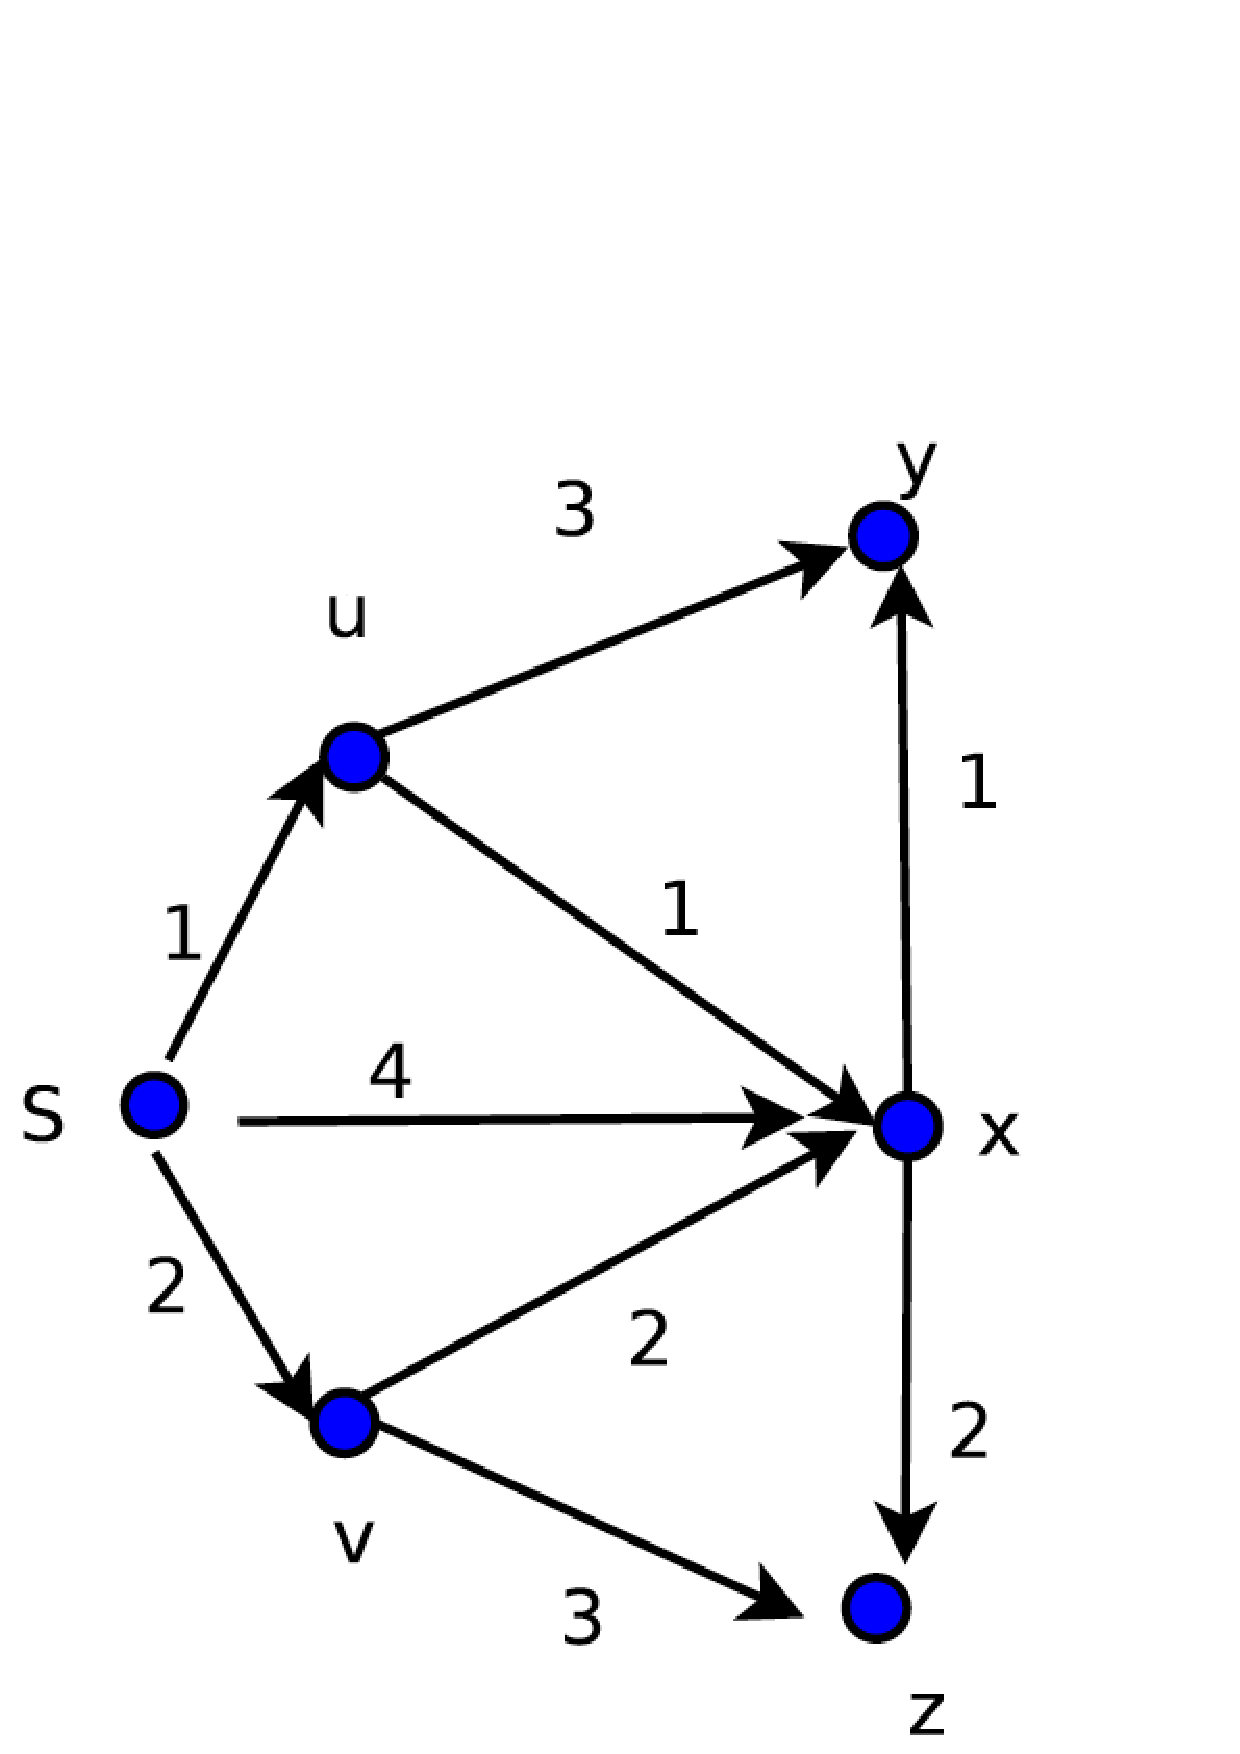
\includegraphics[width=0.9\textwidth]{L7-shortestpathexample.png}
 
\begin{tikzpicture}[auto,swap,scale=0.75]
% 
%    \foreach \pos/\name in {{(0,0)/s}, {(2,2)/u}, {(2,-2)/v}, {(5,0)/x}, {(5,-3)/z}, {(5,3)/y}}
%        \node[vertex,fill=blue!20] (\name) at \pos {$\name$};
%        
%        
%    \foreach \source/\dest/\weight in {s/u/1, s/v/2, s/x/4,   u/y/3,  u/x/1, x/y/1, v/x/2, v/z/3, x/z/2 } 
%            \path[edge] (\source) -- node[weight] {\tiny $\weight$} (\dest);
%	
%\end{tikzpicture} 
%		

  	\def\dx{-6};
 	\def\dy{-1.25};	
    \foreach \pos/\name in {{(0+\dx,0+\dy)/s}, {(2+\dx,1.4+\dy)/u}, {(2+\dx,-1.4+\dy)/v}, {(4+\dx,0+\dy)/x}, {(4+\dx,-2.5+\dy)/t}, {(4+\dx,2.5+\dy)/y}}
        \node[middlevertex,fill=blue!20] (\name) at \pos {$\name$};
        
        
    \foreach \source/\dest/\weight in {s/u/1, s/v/2, s/x/4,   u/y/3,  u/x/1, x/y/1, v/x/2, v/t/3, x/t/2 } 
            \path[edge] (\source) -- node[weight] {\tiny $\weight$} (\dest);
	
 
% \end{minipage}
% \begin{minipage}{0.45\textwidth}

%  \includegraphics[width=\textwidth]{L7-Dijkstraexample.png}
 
 %\begin{tikzpicture}[scale=0.8, auto,swap]
  
  	\def\d{0.7};
	
	%draw index 
 \def\dy{1};
 \def\dx{0};

    \foreach \i/\num/\name in { 1/k=0/, 2/1/s1,3/2/s2,4/3/s3,5/4/s4,6/5/}{
           \node[blue,thick] (\name) at (\i*\d+\d/2 + \dx*\d - \d, \d/2 + \dy * \d) {\tt \num};
    }

 \def\dy{0};
 \def\dx{0};
    \foreach \i/\num/\name in { 1/s/s1,2/u/s2,3/v/s3,4/x/s4, 5/y/,6/t/}{
         \node[blue,thick] (\name) at ( -1*\d+\d/2,  0.0 - \i*\d + \d/2 - \dy * \d + \d){$\num$};
    }

    
%score	
 \def\dy{0};
 \def\dx{0};
    \foreach \i/\num/\name in { 0/0/,1/0/S1,2/0/S2,3/0/,4/0/,5/0/}{
             \draw[  thick ] (\i*\d + \dx*\d,  0+ \dy*\d) rectangle (\i*\d+\d + \dx*\d, \d + \dy*\d);
         \node (\name) at (\i*\d+\d/2 + \dx*\d, \d/2 + \dy*\d) {\tiny $\num$};
    }



%   \draw[blue,ultra thick] (S1) circle[radius=\d/2];
%   \draw[blue,ultra thick] (S2) circle[radius=\d/2];
%   \draw[blue,ultra thick] (L) circle[radius=\d/2];
%
    
       
 \def\dy{-1};
 \def\dx{0};
    \foreach \i/\num/\name in { 0/-/,1/1/S1,2/1/,3//S3,4//,5//}{
             \draw[  thick ] (\i*\d + \dx*\d,  0+ \dy*\d) rectangle (\i*\d+\d + \dx*\d, \d + \dy*\d);
         \node (\name) at (\i*\d+\d/2 + \dx*\d, \d/2 + \dy*\d) {\tiny $\num$};
    }
 
      \draw[red,ultra thick] (S1) circle[radius=\d/2];
   
    
 \def\dy{-2};
 \def\dx{0};
    \foreach \i/\num/\name in { 0/-/,1/2/,2/2/S1,3//S3,4//,5//}{
             \draw[  thick ] (\i*\d + \dx*\d,  0+ \dy*\d) rectangle (\i*\d+\d + \dx*\d, \d + \dy*\d);
         \node (\name) at (\i*\d+\d/2 + \dx*\d, \d/2 + \dy*\d) {\tiny $\num$};
    }
       \draw[red,ultra thick] (S1) circle[radius=\d/2];
 
    
  \def\dy{-3};
 \def\dx{0};
    \foreach \i/\num/\name in { 0/-/,1/4/,2/2/S1,3//S3,4//,5//}{
             \draw[  thick ] (\i*\d + \dx*\d,  0+ \dy*\d) rectangle (\i*\d+\d + \dx*\d, \d + \dy*\d);
         \node (\name) at (\i*\d+\d/2 + \dx*\d, \d/2 + \dy*\d) {\tiny $\num$};
    }
       \draw[red,ultra thick] (S1) circle[radius=\d/2];
  
  \def\dy{-4};
 \def\dx{0};
    \foreach \i/\num/\name in { 0/-/,1/-/,2/4/,3//S1,4//,5//}{
             \draw[  thick ] (\i*\d + \dx*\d,  0+ \dy*\d) rectangle (\i*\d+\d + \dx*\d, \d + \dy*\d);
         \node (\name) at (\i*\d+\d/2 + \dx*\d, \d/2 + \dy*\d) {\tiny $\num$};
    }
%         \draw[red,ultra thick] (S1) circle[radius=\d/2];

  \def\dy{-5};
 \def\dx{0};
    \foreach \i/\num/\name in { 0/-/,1/-/,2/5/,3//S3,4//S1,5//}{
             \draw[  thick ] (\i*\d + \dx*\d,  0+ \dy*\d) rectangle (\i*\d+\d + \dx*\d, \d + \dy*\d);
         \node (\name) at (\i*\d+\d/2 + \dx*\d, \d/2 + \dy*\d) {\tiny $\num$};
    }
%        \draw[red,ultra thick] (S1) circle[radius=\d/2];
 


%draw blue rectangles 

% \def\dy{-1};
% \def\dx{0};
%    \foreach \i/\num/\name in { 2/1/,3/1/S3,4/1/,5/1/}{
%             \draw[  thick, green ] (\i*\d + \dx*\d,  0+ \dy*\d) rectangle (\i*\d+\d + \dx*\d, \d + \dy*\d);
%    }
% 
     
    
% \def\dy{-2};
% \def\dx{0};
%    \foreach \i/\num/\name in { 3/2/S3,4/2/,5/2/}{
%             \draw[  thick, green  ] (\i*\d + \dx*\d,  0+ \dy*\d) rectangle (\i*\d+\d + \dx*\d, \d + \dy*\d);
%      }
% 
%    
%  \def\dy{-3};
% \def\dx{0};
%    \foreach \i/\num/\name in { 3/2/S3,4/2/,5/2/}{
%             \draw[  thick, green ] (\i*\d + \dx*\d,  0+ \dy*\d) rectangle (\i*\d+\d + \dx*\d, \d + \dy*\d);
%    }
 
%   \def\dy{-4};
% \def\dx{0};
%    \foreach \i/\num/\name in { 4/3/,5/3/}{
%             \draw[  thick, green ] (\i*\d + \dx*\d,  0+ \dy*\d) rectangle (\i*\d+\d + \dx*\d, \d + \dy*\d);
%    }
% 
%  \def\dy{-5};
% \def\dx{0};
%    \foreach \i/\num/\name in {5/4/}{
%             \draw[  thick, green ] (\i*\d + \dx*\d,  0+ \dy*\d) rectangle (\i*\d+\d + \dx*\d, \d + \dy*\d);
%     }

\end{tikzpicture} 
 
% \end{minipage}
\end{figure}

}

\frame{
\frametitle{Final step  } 

\begin{figure}
% \begin{minipage}{0.40\textwidth}
%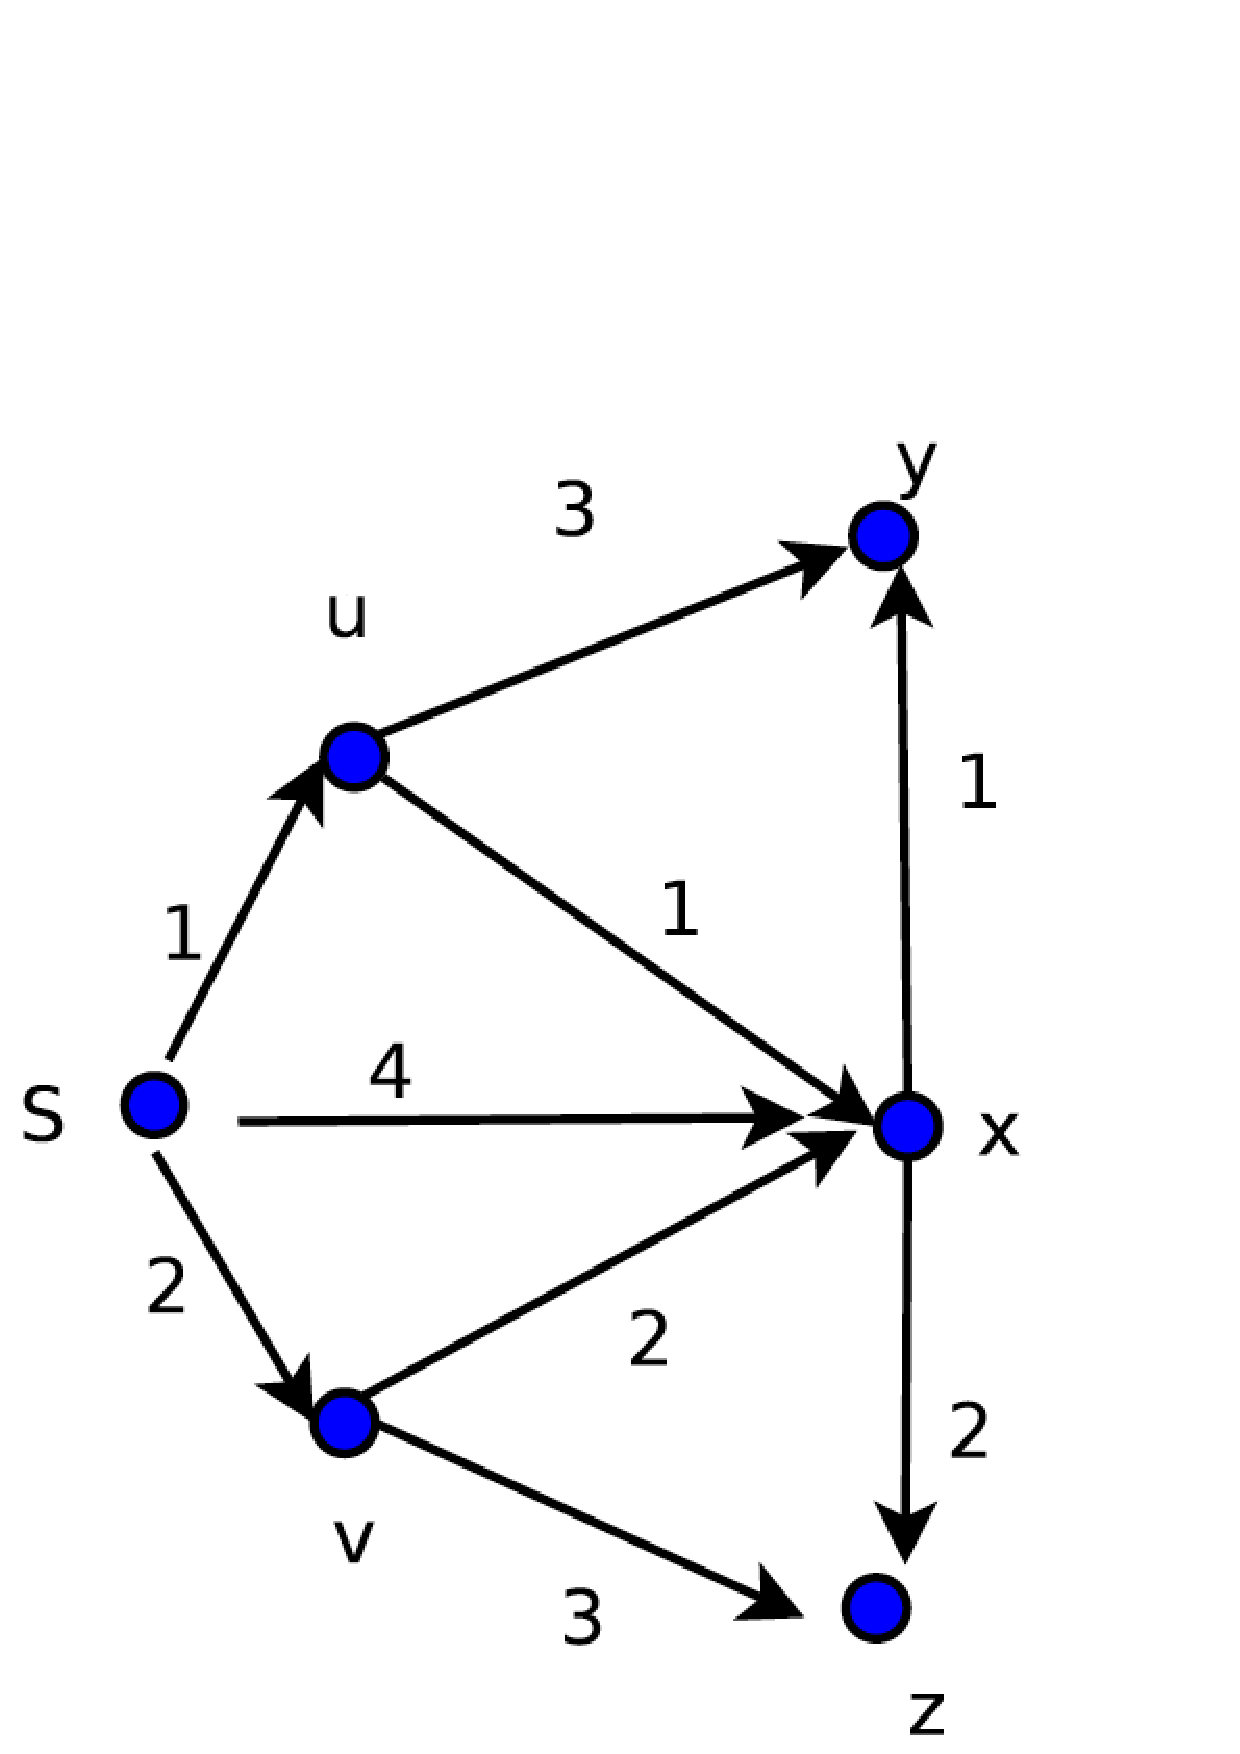
\includegraphics[width=\textwidth]{L7-shortestpathexample.png}

\begin{tikzpicture}[auto,swap, scale=0.75]

 	\def\dx{-6};
 	\def\dy{-1.25};	
    \foreach \pos/\name in {{(0+\dx,0+\dy)/s}, {(2+\dx,1.4+\dy)/u}, {(2+\dx,-1.4+\dy)/v}, {(4+\dx,0+\dy)/x}, {(4+\dx,-2.5+\dy)/t}, {(4+\dx,2.5+\dy)/y}}
        \node[middlevertex,fill=blue!20] (\name) at \pos {$\name$};
        
        
    \foreach \source/\dest/\weight in {s/u/1, s/v/2, s/x/4,   u/y/3,  u/x/1, x/y/1, v/x/2, v/t/3, x/t/2 } 
            \path[edge] (\source) -- node[weight] {\tiny $\weight$} (\dest);

    \foreach \source/\dest/\weight in {s/u/1, s/v/2,    u/x/1, x/y/1, x/t/2 } 
            \path[edge, green, ultra thick] (\source) -- node[weight] {} (\dest);
	
%\end{tikzpicture} 
				
 
% \end{minipage}
% \begin{minipage}{0.45\textwidth}

%  \includegraphics[width=\textwidth]{L7-Dijkstraexample.png}
 
% \begin{tikzpicture}[auto,swap]
  
  	\def\d{0.7};
	
	%draw index 
 \def\dy{1};
 \def\dx{0};

    \foreach \i/\num/\name in { 1/k=0/, 2/1/s1,3/2/s2,4/3/s3,5/4/s4,6/5/}{
           \node[blue,thick] (\name) at (\i*\d+\d/2 + \dx*\d - \d, \d/2 + \dy * \d) {\tt \num};
    }

 \def\dy{0};
 \def\dx{0};
    \foreach \i/\num/\name in { 1/s/s1,2/u/s2,3/v/s3,4/x/s4, 5/y/,6/t/}{
         \node[blue,thick] (\name) at ( -1*\d+\d/2,  0.0 - \i*\d + \d/2 - \dy * \d + \d){$\num$};
    }

    
%score	
 \def\dy{0};
 \def\dx{0};
    \foreach \i/\num/\name in { 0/0/,1/0/S1,2/0/S2,3/0/,4/0/,5/0/}{
             \draw[  thick ] (\i*\d + \dx*\d,  0+ \dy*\d) rectangle (\i*\d+\d + \dx*\d, \d + \dy*\d);
         \node (\name) at (\i*\d+\d/2 + \dx*\d, \d/2 + \dy*\d) {\tiny $\num$};
    }



%   \draw[blue,ultra thick] (S1) circle[radius=\d/2];
%   \draw[blue,ultra thick] (S2) circle[radius=\d/2];
%   \draw[blue,ultra thick] (L) circle[radius=\d/2];
%
    
        
 \def\dy{-1};
 \def\dx{0};
    \foreach \i/\num/\name in { 0/-/,1/1/S1,2/1/,3/1/S3,4/1/,5/1/}{
             \draw[  thick ] (\i*\d + \dx*\d,  0+ \dy*\d) rectangle (\i*\d+\d + \dx*\d, \d + \dy*\d);
         \node (\name) at (\i*\d+\d/2 + \dx*\d, \d/2 + \dy*\d) {\tiny $\num$};
    }
 
    %  \draw[red,ultra thick] (S1) circle[radius=\d/2];
   
    
 \def\dy{-2};
 \def\dx{0};
    \foreach \i/\num/\name in { 0/-/,1/2/,2/2/S1,3/2/S3,4/2/,5/2/}{
             \draw[  thick ] (\i*\d + \dx*\d,  0+ \dy*\d) rectangle (\i*\d+\d + \dx*\d, \d + \dy*\d);
         \node (\name) at (\i*\d+\d/2 + \dx*\d, \d/2 + \dy*\d) {\tiny $\num$};
    }
 
    
  \def\dy{-3};
 \def\dx{0};
    \foreach \i/\num/\name in { 0/-/,1/4/,2/2/S1,3/2/S3,4/2/,5/2/}{
             \draw[  thick ] (\i*\d + \dx*\d,  0+ \dy*\d) rectangle (\i*\d+\d + \dx*\d, \d + \dy*\d);
         \node (\name) at (\i*\d+\d/2 + \dx*\d, \d/2 + \dy*\d) {\tiny $\num$};
    }
   
  \def\dy{-4};
 \def\dx{0};
    \foreach \i/\num/\name in { 0/-/,1/-/,2/4/,3/3/S1,4/3/,5/3/}{
             \draw[  thick ] (\i*\d + \dx*\d,  0+ \dy*\d) rectangle (\i*\d+\d + \dx*\d, \d + \dy*\d);
         \node (\name) at (\i*\d+\d/2 + \dx*\d, \d/2 + \dy*\d) {\tiny $\num$};
    }

  \def\dy{-5};
 \def\dx{0};
    \foreach \i/\num/\name in { 0/-/,1/-/,2/5/,3/4/S3,4/4/S1,5/4/}{
             \draw[  thick ] (\i*\d + \dx*\d,  0+ \dy*\d) rectangle (\i*\d+\d + \dx*\d, \d + \dy*\d);
         \node (\name) at (\i*\d+\d/2 + \dx*\d, \d/2 + \dy*\d) {\tiny $\num$};
    }
 

\end{tikzpicture} 
 
% \end{minipage}
\end{figure}

\begin{itemize}
	\item Recall that the collection of the shortest paths from $s$ to all nodes form a shortest path tree. 
\end{itemize}

}

%\frame{
%	\frametitle{multistage decision process} 
%	
%\begin{figure}
%\begin{tikzpicture}[auto,swap,scale=0.6]
%
% 	\def\dx{-11};
% 	\def\dy{-1.8};	
%    \foreach \pos/\name in {{(0+\dx,0+\dy)/s}, {(2+\dx,1.4+\dy)/u}, {(2+\dx,-1.4+\dy)/v}, {(4+\dx,0+\dy)/x}, {(4+\dx,-2.5+\dy)/t}, {(4+\dx,2.5+\dy)/y}}
%        \node[middlevertex,fill=blue!20] (\name) at \pos {$\name$};
%        
%        
%    \foreach \source/\dest/\weight in {s/u/1, s/v/2, s/x/4,   u/y/3,  u/x/1, x/y/1, v/x/2, v/t/3, x/t/2 } 
%            \path[edge] (\source) -- node[weight] {\tiny $\weight$} (\dest);
%
%    \foreach \source/\dest/\weight in {s/u/1, s/v/2,    u/x/1, x/y/1, x/t/2 } 
%            \path[edge, green, ultra thick] (\source) -- node[weight] {} (\dest);
%
%
%
%
%    \def\dx{0};
%   \def\dy{0.9} 
%
%%Tree
%
%	\def\d{1.5}; 
%	\def\e{2};
%	\def\f{1.0};
%	\def\h{2};
%
%% Label
%
%
%	
%   \node at ( -2.2*\e, -\h * 0.5)  {\tiny $x_1=x/u/v$};  
%%   \node at ( -2.2*\e, -\h * 1.5)  {\tiny $x_2=x/v/y/t$};  
%
%%layer 1	
%    \foreach \pos/\name/\label in {{(0,0)/root/}} 
%        \node[tinyvertex,draw=black, fill=white!20] (\name) at \pos {};
%%layer 2	
%    \foreach \pos/\name/\label in { {(-1.5*\d, -1*\h)/L11/}, {(-0*\d,-1*\h)/L12/},{(1.5*\d, -1*\h)/L14/}}  
%        \node[tinyvertex,draw=black, fill=white!20] (\name) at \pos {};	
%
% % Edges 
% 	%layer 1
%  	\foreach \source/ \dest /\weight in {root/L11/, root/L12/, root/L14/ }         
%		\path[undirectededge] (\source) -- node[weight] { } (\dest);
%
%
%   %Label
%   \def\s{1.05};  
%   \def\t{0.4};  
%   \node[] at (0 + \s, 0) {\tiny $X=?????$}; 
%   \node[] at (0 + \s, 0 - \t) {\tiny ${\tiny P_{0}}$  }; 
% 
%  %layer 1
%    \def\s{0.75};  
%   \node[] at (-1.5*\d + \s, -1*\h ) {\tiny $x????$}; 
%   \node[] at (-1.5*\d + \s, -1*\h  - \t) {\tiny ${\tiny P_{1}}$ }; 
%
%   \node[] at (-0*\d + \s, -1*\h ) {\tiny $u????$}; 
%   \node[] at (-0*\d + \s, -1*\h  - \t) {\tiny ${\tiny P_{2}}$}; 
%  
%   \node[] at (1.5*\d + \s, -1*\h ) {\tiny $v????$}; 
%   \node[] at (1.5*\d + \s, -1*\h  - \t) {\tiny ${\tiny P_{3}}$}; 
%
%    		
%\end{tikzpicture} 
%\end{figure}
%
%\begin{itemize}
%	\item The construction of the shortest path tree rooted at $s$ is a multistage decision process: The tree is described as $X=[x_1, x_2, ..., x_5]$, where $x_i\in V$ represents the  node selected at the $i$-th stage. 
%	\item At the first stage, the dynamic programming algorithm enumerates all options as we have no idea of the optimal decision. 
%\end{itemize}
%
%	
%}



\frame{
	\begin{block}{}
	Greedy-selection property in  version 2 
	\end{block} 
}

\frame{
	\frametitle{Greedy-selection rule in multistage decision process} 
	
\begin{figure}
\begin{tikzpicture}[auto,swap,scale=0.6]

 	\def\dx{-11};
 	\def\dy{-1.8};	
    \foreach \pos/\name in {{(0+\dx,0+\dy)/s}, {(2+\dx,1.4+\dy)/u}, {(2+\dx,-1.4+\dy)/v}, {(4+\dx,0+\dy)/x}, {(4+\dx,-2.5+\dy)/t}, {(4+\dx,2.5+\dy)/y}}
        \node[middlevertex,fill=blue!20] (\name) at \pos {$\name$};
        
        
    \foreach \source/\dest/\weight in {s/u/1, s/v/2, s/x/4,   u/y/3,  u/x/1, x/y/1, v/x/2, v/t/3, x/t/2 } 
            \path[edge] (\source) -- node[weight] {\tiny $\weight$} (\dest);

    \foreach \source/\dest/\weight in {s/u/1, s/v/2,    u/x/1, x/y/1, x/t/2 } 
            \path[edge, green, ultra thick] (\source) -- node[weight] {} (\dest);




    \def\dx{0};
   \def\dy{0.9} 

%Tree

	\def\d{1.5}; 
	\def\e{2};
	\def\f{1.0};
	\def\h{2};

% Label


	
   \node at ( -2.2*\e, -\h * 0.5)  {\tiny $x_1=x/u/v$};  
   \node at ( -2.2*\e, -\h * 1.5)  {\tiny $x_2=x/v/y/t$};  

%layer 1	
    \foreach \pos/\name/\label in {{(0,0)/root/}} 
        \node[tinyvertex,draw=black, fill=white!20] (\name) at \pos {};
%layer 2	
    \foreach \pos/\name/\label in { {(-1.5*\d, -1*\h)/L11/}, {(-0*\d,-1*\h)/L12/},{(1.5*\d, -1*\h)/L14/}}  
        \node[tinyvertex,draw=black, fill=white!20] (\name) at \pos {};	
%layer 3	
    \foreach \pos/\name/\label in { {(-1.5*\e, -2*\h)/L21/}, {(-0.5*\e,  -2*\h)/L22/}, {(0.5*\e,  -2*\h)/L23/}, {(1.5*\e, -2*\h)/L24/}}  
        \node[tinyvertex,draw=black, fill=white!20] (\name) at \pos {};	

 % Edges 
 	%layer 1
  	\foreach \source/ \dest /\weight in {root/L11/, root/L12/, root/L14/ }         
		\path[undirectededge] (\source) -- node[weight] { } (\dest);
	%layer 2
	 \foreach \source/ \dest /\weight in {L12/L21/, L12/L22/, L12/L23/, L12/L24/}         
		\path[undirectededge] (\source) -- node[weight] { } (\dest);


	 \foreach \source/ \dest /\weight in {root/L12/, L12/L21/}         
		\path[undirectededge, red, ultra thick] (\source) -- node[weight] { } (\dest);


   %Label
   \def\s{1.05};  
   \def\t{0.4};  
   \node[] at (0 + \s, 0) {\tiny $X=?????$}; 
   \node[] at (0 + \s, 0 - \t) {\tiny ${\tiny P_{0}}$  }; 
 
  %layer 1
    \def\s{0.75};  
   \node[] at (-1.5*\d + \s, -1*\h ) {\tiny $x????$}; 
   \node[] at (-1.5*\d + \s, -1*\h  - \t) {\tiny ${\tiny P_{1}}$ }; 

   \node[] at (-0*\d + \s, -1*\h ) {\tiny $u????$}; 
   \node[] at (-0*\d + \s, -1*\h  - \t) {\tiny ${\tiny P_{2}}$}; 
  
   \node[] at (1.5*\d + \s, -1*\h ) {\tiny $v????$}; 
   \node[] at (1.5*\d + \s, -1*\h  - \t) {\tiny ${\tiny P_{3}}$}; 


%layer 2
   \node[] at (-1.5*\e  + \s, -2*\h ) {\tiny $ux???$  }; 
   \node[] at (-1.5*\e  + \s, -2*\h  - \t) {\tiny ${\tiny P_{4}}$   }; 

   \node[] at (-.5*\e  + \s, -2*\h ) {\tiny $uv???$ }; 
   \node[] at (-.5*\e  + \s, -2*\h  - \t) {\tiny ${\tiny P_{5}}$ }; 

   \node[] at (.5*\e + \s, -2*\h ) {\tiny $uy???$}; 
   \node[] at (.5*\e + \s, -2*\h  - \t) {\tiny ${\tiny P_{6}}$   }; 

   \node[] at (1.5*\e + \s, -2*\h ) {\tiny $ut???$}; 
   \node[] at (1.5*\e + \s, -2*\h  - \t) {\tiny ${\tiny P_{7}}$  }; 

  \node[] at (-1.8*\e + \s, -2.5*\h ) {......}; 

    		
\end{tikzpicture} 
\end{figure}

\begin{itemize}
	\item The construction of the shortest path tree rooted at $s$ is a multistage decision process: The tree is described as $X=[x_1, x_2, ..., x_5]$, where $x_i\in V$ represents the  node selected at the $i$-th stage. The Dijkstra's algorithm  selects the nearest node adjacent to ``explored" nodes at each stage. 
	\item This greedy-selection rule works due to the following two observations of {\sc Bellman\_Ford} algorithm, namely,  some operations are redundant, and  the nearest node adjacent to ``explored" nodes has its shortest distance determined. 
\end{itemize}

	
}

\frame{
\frametitle{Redundant calculations in {\sc Bellman\_Ford} algorithm} 
% \begin{footnotesize}
%  $OPT(k, v) = \min \begin{cases} 
%                       OPT( k-1, v) \\
%                       \min_{<u,v>\in E} OPT( k-1, u) + d_{u,v}  \\
%                      \end{cases} $
% \end{footnotesize}

 \begin{itemize}
\item At the $k$-th step, let's consider a special node $v^*$, the nearest node from $s$ via at most $k-1$ edges, i.e. 
\[
OPT(  v^*, k-1 ) = min_v OPT( v, k-1 )
\] 

\item Consider the optimal substructure property for $v^*$, i.e. 
\begin{small} 
\[
OPT(v^*, k ) = \min \begin{cases} 
                      OPT(  v^*, k-1) \\
                      \min_{<u,v^*>\in E} \{ OPT( u, k-1 ) + d_{u, v^*} \}  \\
                     \end{cases} 
\]                     
\end{small} 

The above equality can be further simplified as: 
\[
OPT( v^*, k ) = OPT(  v^*, k-1 ) 
\]
(Why? $OPT(  u, k-1 )\geq OPT(v^*, k-1)$ and $d_{u,v^*} \geq 0$.) 
\end{itemize}
}

\frame{
\frametitle{The meaning of $OPT(v^*, k) = OPT( v^*, k-1)$ for $k=2$} 
\begin{figure}
% \begin{minipage}{0.40\textwidth}
%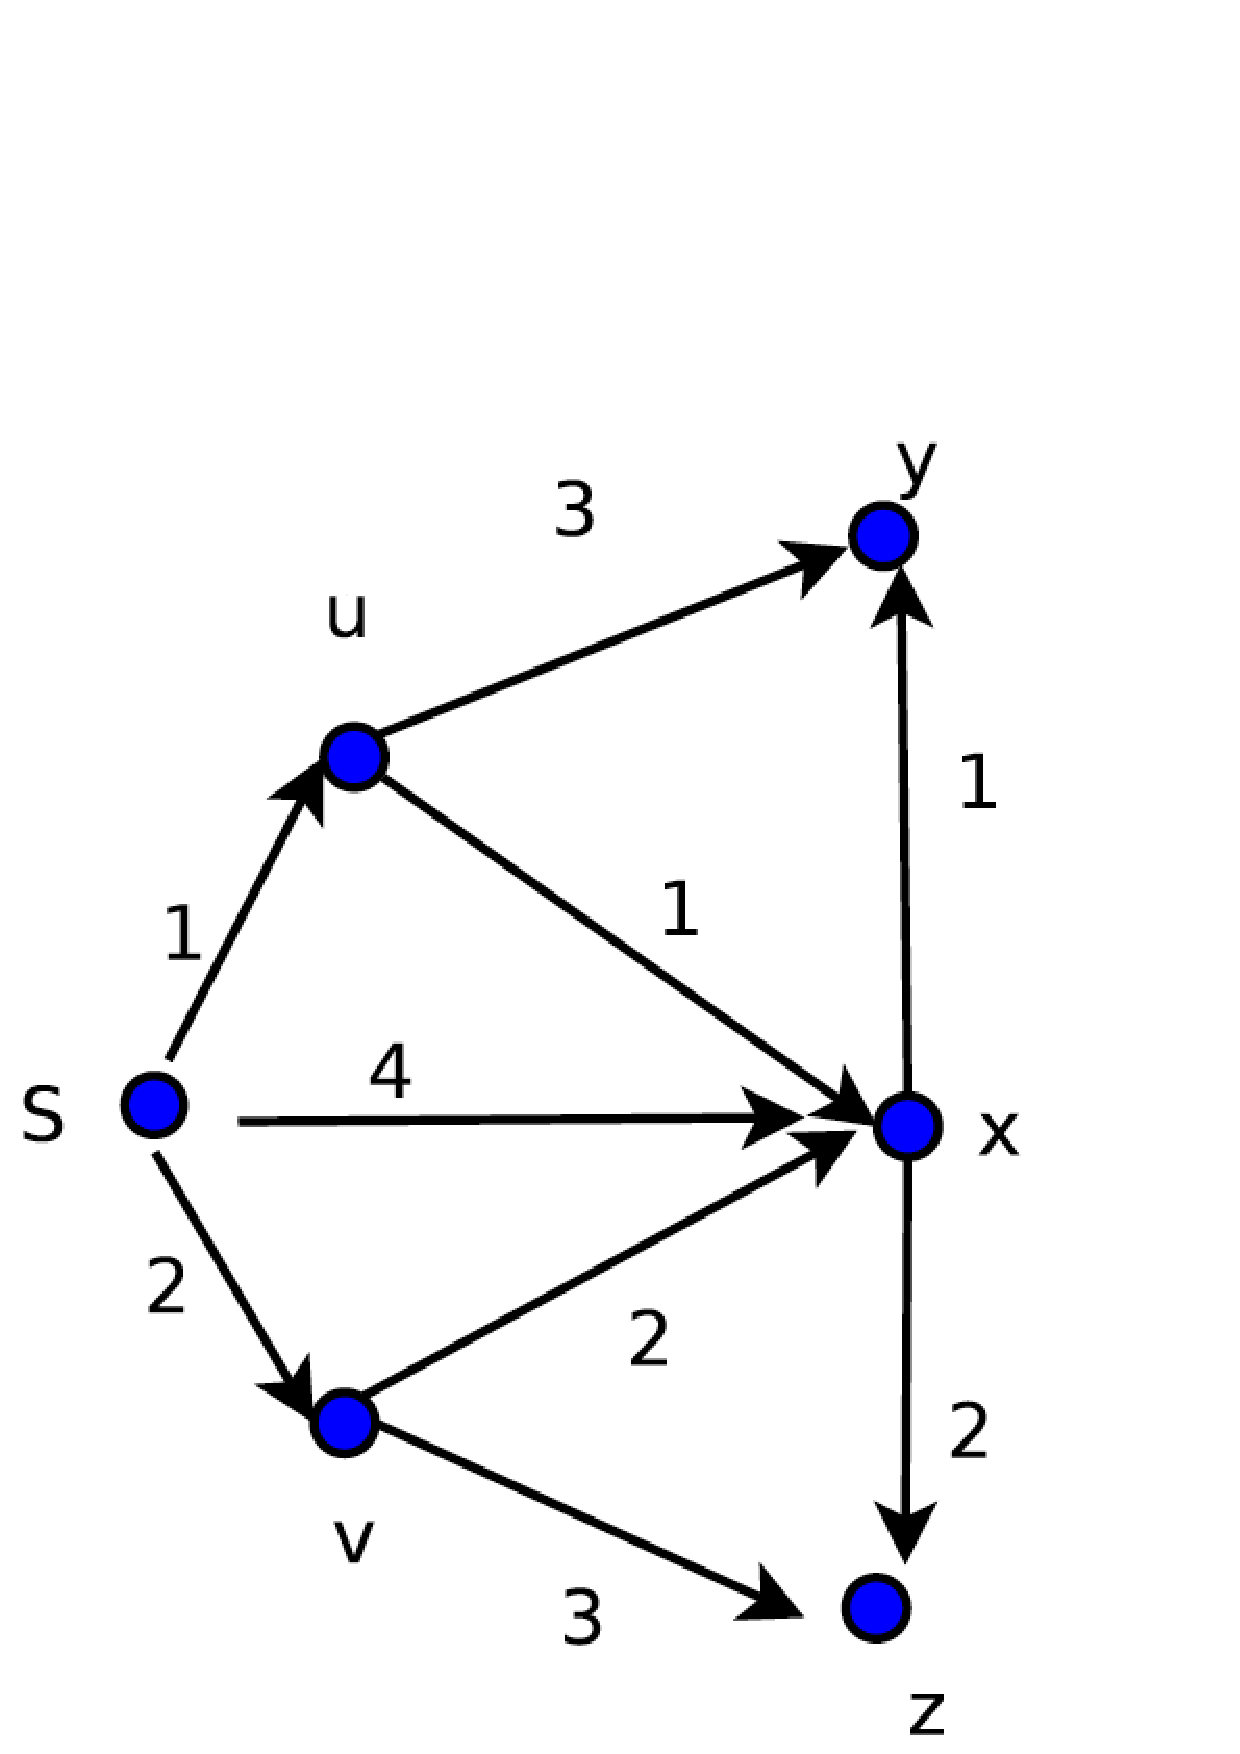
\includegraphics[width=0.9\textwidth]{L7-shortestpathexample.png}
 
\begin{tikzpicture}[auto,swap,scale=0.65]
% 
%    \foreach \pos/\name in {{(0,0)/s}, {(2,2)/u}, {(2,-2)/v}, {(5,0)/x}, {(5,-3)/z}, {(5,3)/y}}
%        \node[vertex,fill=blue!20] (\name) at \pos {$\name$};
%        
%        
%    \foreach \source/\dest/\weight in {s/u/1, s/v/2, s/x/4,   u/y/3,  u/x/1, x/y/1, v/x/2, v/z/3, x/z/2 } 
%            \path[edge] (\source) -- node[weight] {\tiny $\weight$} (\dest);
%	
%\end{tikzpicture} 
%		

  	\def\dx{-6};
 	\def\dy{-1.25};	
    \foreach \pos/\name in {{(0+\dx,0+\dy)/s}, {(2+\dx,1.4+\dy)/u}, {(2+\dx,-1.4+\dy)/v}, {(4+\dx,0+\dy)/x}, {(4+\dx,-2.5+\dy)/t}, {(4+\dx,2.5+\dy)/y}}
        \node[middlevertex,fill=blue!20] (\name) at \pos {$\name$};
        
        
    \foreach \source/\dest/\weight in {s/u/1, s/v/2, s/x/4,   u/y/3,  u/x/1, x/y/1, v/x/2, v/t/3, x/t/2 } 
            \path[edge] (\source) -- node[weight] {\tiny $\weight$} (\dest);
	
 
% \end{minipage}
% \begin{minipage}{0.45\textwidth}

%  \includegraphics[width=\textwidth]{L7-Dijkstraexample.png}
 
 %\begin{tikzpicture}[scale=0.8, auto,swap]
  
  	\def\d{0.7};
	
	%draw index 
 \def\dy{1};
 \def\dx{0};

    \foreach \i/\num/\name in { 1/k=0/, 2/1/s1,3/2/s2,4/3/s3,5/4/s4,6/5/}{
           \node[blue,thick] (\name) at (\i*\d+\d/2 + \dx*\d - \d, \d/2 + \dy * \d) {\tt \num};
    }

 \def\dy{0};
 \def\dx{0};
    \foreach \i/\num/\name in { 1/s/s1,2/u/s2,3/v/s3,4/x/s4, 5/y/,6/t/}{
         \node[blue,thick] (\name) at ( -1*\d+\d/2,  0.0 - \i*\d + \d/2 - \dy * \d + \d){$\num$};
    }

    
%score	
 \def\dy{0};
 \def\dx{0};
    \foreach \i/\num/\name in { 0/0/,1/0/S1,2/0/S2,3/0/,4/0/,5/0/}{
             \draw[  thick ] (\i*\d + \dx*\d,  0+ \dy*\d) rectangle (\i*\d+\d + \dx*\d, \d + \dy*\d);
         \node (\name) at (\i*\d+\d/2 + \dx*\d, \d/2 + \dy*\d) {\tiny $\num$};
    }



%   \draw[blue,ultra thick] (S1) circle[radius=\d/2];
%   \draw[blue,ultra thick] (S2) circle[radius=\d/2];
%   \draw[blue,ultra thick] (L) circle[radius=\d/2];
%
    
       
 \def\dy{-1};
 \def\dx{0};
    \foreach \i/\num/\name in { 0/-/,1/1/S1,2/1/,3/1/S3,4/1/,5/1/}{
             \draw[  thick ] (\i*\d + \dx*\d,  0+ \dy*\d) rectangle (\i*\d+\d + \dx*\d, \d + \dy*\d);
         \node (\name) at (\i*\d+\d/2 + \dx*\d, \d/2 + \dy*\d) {\tiny $\num$};
    }
 
      \draw[red,ultra thick] (S1) circle[radius=\d/2];
   
    
 \def\dy{-2};
 \def\dx{0};
    \foreach \i/\num/\name in { 0/-/,1/2/,2//S1,3//S3,4//,5//}{
             \draw[  thick ] (\i*\d + \dx*\d,  0+ \dy*\d) rectangle (\i*\d+\d + \dx*\d, \d + \dy*\d);
         \node (\name) at (\i*\d+\d/2 + \dx*\d, \d/2 + \dy*\d) {\tiny $\num$};
    }
%       \draw[red,ultra thick] (S1) circle[radius=\d/2];
 
    
  \def\dy{-3};
 \def\dx{0};
    \foreach \i/\num/\name in { 0/-/,1/4/,2//S1,3//S3,4//,5//}{
             \draw[  thick ] (\i*\d + \dx*\d,  0+ \dy*\d) rectangle (\i*\d+\d + \dx*\d, \d + \dy*\d);
         \node (\name) at (\i*\d+\d/2 + \dx*\d, \d/2 + \dy*\d) {\tiny $\num$};
    }
%       \draw[red,ultra thick] (S1) circle[radius=\d/2];
  
  \def\dy{-4};
 \def\dx{0};
    \foreach \i/\num/\name in { 0/-/,1/-/,2//,3//S1,4//,5//}{
             \draw[  thick ] (\i*\d + \dx*\d,  0+ \dy*\d) rectangle (\i*\d+\d + \dx*\d, \d + \dy*\d);
         \node (\name) at (\i*\d+\d/2 + \dx*\d, \d/2 + \dy*\d) {\tiny $\num$};
    }
%         \draw[red,ultra thick] (S1) circle[radius=\d/2];

  \def\dy{-5};
 \def\dx{0};
    \foreach \i/\num/\name in { 0/-/,1/-/,2//,3//S3,4//S1,5//}{
             \draw[  thick ] (\i*\d + \dx*\d,  0+ \dy*\d) rectangle (\i*\d+\d + \dx*\d, \d + \dy*\d);
         \node (\name) at (\i*\d+\d/2 + \dx*\d, \d/2 + \dy*\d) {\tiny $\num$};
    }
%        \draw[red,ultra thick] (S1) circle[radius=\d/2];
 


%draw blue rectangles 

 \def\dy{-1};
 \def\dx{0};
    \foreach \i/\num/\name in { 2/1/,3/1/S3,4/1/,5/1/}{
             \draw[  thick, green ] (\i*\d + \dx*\d,  0+ \dy*\d) rectangle (\i*\d+\d + \dx*\d, \d + \dy*\d);
    }
 
     
    
% \def\dy{-2};
% \def\dx{0};
%    \foreach \i/\num/\name in { 3/2/S3,4/2/,5/2/}{
%             \draw[  thick, green  ] (\i*\d + \dx*\d,  0+ \dy*\d) rectangle (\i*\d+\d + \dx*\d, \d + \dy*\d);
%      }
% 
%    
%  \def\dy{-3};
% \def\dx{0};
%    \foreach \i/\num/\name in { 3/2/S3,4/2/,5/2/}{
%             \draw[  thick, green ] (\i*\d + \dx*\d,  0+ \dy*\d) rectangle (\i*\d+\d + \dx*\d, \d + \dy*\d);
%    }
% 
%   \def\dy{-4};
% \def\dx{0};
%    \foreach \i/\num/\name in { 4/3/,5/3/}{
%             \draw[  thick, green ] (\i*\d + \dx*\d,  0+ \dy*\d) rectangle (\i*\d+\d + \dx*\d, \d + \dy*\d);
%    }
% 
%  \def\dy{-5};
% \def\dx{0};
%    \foreach \i/\num/\name in {5/4/}{
%             \draw[  thick, green ] (\i*\d + \dx*\d,  0+ \dy*\d) rectangle (\i*\d+\d + \dx*\d, \d + \dy*\d);
%     }

\end{tikzpicture} 
 
% \end{minipage}
\end{figure}

\begin{itemize}
\item  Intuitively $v^*$ (in red circles) can be treated as \textcolor{red}{\bf has already been explored using at most $(k-1)$ edges}, and the distance will not change afterwards.
  Thus, the calculations of $OPT(v^*, k)$ (in green rectangles) are in fact redundant.
\item In other words, it suffices to calculate \begin{small} $OPT[v, k] = \min \begin{cases}
			OPT[v, k-1], \\
			\min_{<u,v>\in E} \{OPT[ u, k-1 ] + d(u,v) \} 
		\end{cases}$
		\end{small} for the \textcolor{red}{\bf unexplored nodes} $v \neq v^*$, including $v, x, y, t$. 
\end{itemize}
}

\frame{
\frametitle{The meaning of $OPT(v^*, k) = OPT( v^*, k-1)$ for $k=3$ } 
\begin{figure}
% \begin{minipage}{0.40\textwidth}
%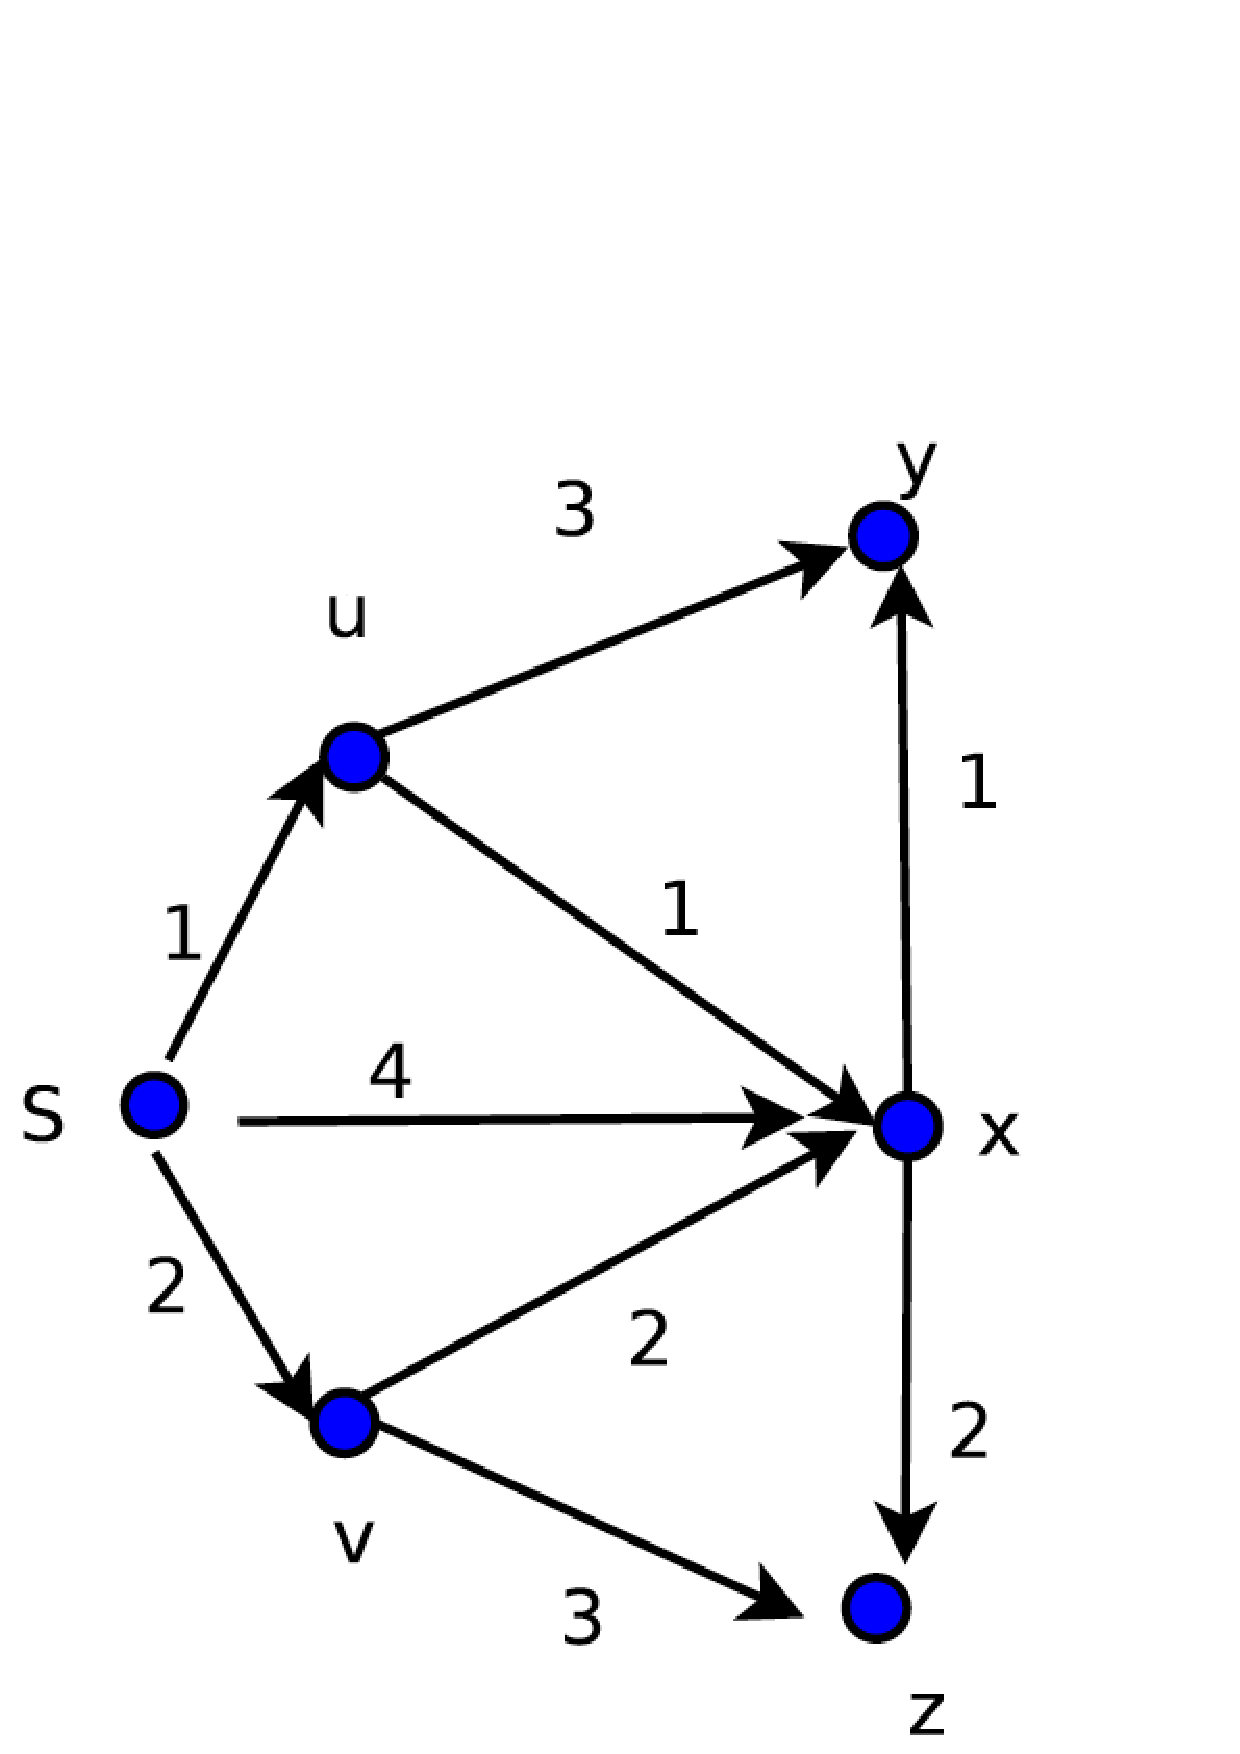
\includegraphics[width=0.9\textwidth]{L7-shortestpathexample.png}
 
\begin{tikzpicture}[auto,swap,scale=0.65]
% 
%    \foreach \pos/\name in {{(0,0)/s}, {(2,2)/u}, {(2,-2)/v}, {(5,0)/x}, {(5,-3)/z}, {(5,3)/y}}
%        \node[vertex,fill=blue!20] (\name) at \pos {$\name$};
%        
%        
%    \foreach \source/\dest/\weight in {s/u/1, s/v/2, s/x/4,   u/y/3,  u/x/1, x/y/1, v/x/2, v/z/3, x/z/2 } 
%            \path[edge] (\source) -- node[weight] {\tiny $\weight$} (\dest);
%	
%\end{tikzpicture} 
%		

  	\def\dx{-6};
 	\def\dy{-1.25};	
    \foreach \pos/\name in {{(0+\dx,0+\dy)/s}, {(2+\dx,1.4+\dy)/u}, {(2+\dx,-1.4+\dy)/v}, {(4+\dx,0+\dy)/x}, {(4+\dx,-2.5+\dy)/t}, {(4+\dx,2.5+\dy)/y}}
        \node[middlevertex,fill=blue!20] (\name) at \pos {$\name$};
        
        
    \foreach \source/\dest/\weight in {s/u/1, s/v/2, s/x/4,   u/y/3,  u/x/1, x/y/1, v/x/2, v/t/3, x/t/2 } 
            \path[edge] (\source) -- node[weight] {\tiny $\weight$} (\dest);
	
 
% \end{minipage}
% \begin{minipage}{0.45\textwidth}

%  \includegraphics[width=\textwidth]{L7-Dijkstraexample.png}
 
 %\begin{tikzpicture}[scale=0.8, auto,swap]
  
  	\def\d{0.7};
	
	%draw index 
 \def\dy{1};
 \def\dx{0};

    \foreach \i/\num/\name in { 1/k=0/, 2/1/s1,3/2/s2,4/3/s3,5/4/s4,6/5/}{
           \node[blue,thick] (\name) at (\i*\d+\d/2 + \dx*\d - \d, \d/2 + \dy * \d) {\tt \num};
    }

 \def\dy{0};
 \def\dx{0};
    \foreach \i/\num/\name in { 1/s/s1,2/u/s2,3/v/s3,4/x/s4, 5/y/,6/t/}{
         \node[blue,thick] (\name) at ( -1*\d+\d/2,  0.0 - \i*\d + \d/2 - \dy * \d + \d){$\num$};
    }

    
%score	
 \def\dy{0};
 \def\dx{0};
    \foreach \i/\num/\name in { 0/0/,1/0/S1,2/0/S2,3/0/,4/0/,5/0/}{
             \draw[  thick ] (\i*\d + \dx*\d,  0+ \dy*\d) rectangle (\i*\d+\d + \dx*\d, \d + \dy*\d);
         \node (\name) at (\i*\d+\d/2 + \dx*\d, \d/2 + \dy*\d) {\tiny $\num$};
    }



%   \draw[blue,ultra thick] (S1) circle[radius=\d/2];
%   \draw[blue,ultra thick] (S2) circle[radius=\d/2];
%   \draw[blue,ultra thick] (L) circle[radius=\d/2];
%
    
       
 \def\dy{-1};
 \def\dx{0};
    \foreach \i/\num/\name in { 0/-/,1/1/S1,2/1/,3/1/S3,4/1/,5/1/}{
             \draw[  thick ] (\i*\d + \dx*\d,  0+ \dy*\d) rectangle (\i*\d+\d + \dx*\d, \d + \dy*\d);
         \node (\name) at (\i*\d+\d/2 + \dx*\d, \d/2 + \dy*\d) {\tiny $\num$};
    }
 
      \draw[red,ultra thick] (S1) circle[radius=\d/2];
   
    
 \def\dy{-2};
 \def\dx{0};
    \foreach \i/\num/\name in { 0/-/,1/2/,2/2/S1,3/2/S3,4/2/,5/2/}{
             \draw[  thick ] (\i*\d + \dx*\d,  0+ \dy*\d) rectangle (\i*\d+\d + \dx*\d, \d + \dy*\d);
         \node (\name) at (\i*\d+\d/2 + \dx*\d, \d/2 + \dy*\d) {\tiny $\num$};
    }
       \draw[red,ultra thick] (S1) circle[radius=\d/2];
 
    
  \def\dy{-3};
 \def\dx{0};
    \foreach \i/\num/\name in { 0/-/,1/4/,2/2/S1,3/2/S3,4/2/,5/2/}{
             \draw[  thick ] (\i*\d + \dx*\d,  0+ \dy*\d) rectangle (\i*\d+\d + \dx*\d, \d + \dy*\d);
         \node (\name) at (\i*\d+\d/2 + \dx*\d, \d/2 + \dy*\d) {\tiny $\num$};
    }
       \draw[red,ultra thick] (S1) circle[radius=\d/2];
  
  \def\dy{-4};
 \def\dx{0};
    \foreach \i/\num/\name in { 0/-/,1/-/,2/4/,3//S1,4//,5//}{
             \draw[  thick ] (\i*\d + \dx*\d,  0+ \dy*\d) rectangle (\i*\d+\d + \dx*\d, \d + \dy*\d);
         \node (\name) at (\i*\d+\d/2 + \dx*\d, \d/2 + \dy*\d) {\tiny $\num$};
    }
%         \draw[red,ultra thick] (S1) circle[radius=\d/2];

  \def\dy{-5};
 \def\dx{0};
    \foreach \i/\num/\name in { 0/-/,1/-/,2/5/,3//S3,4//S1,5//}{
             \draw[  thick ] (\i*\d + \dx*\d,  0+ \dy*\d) rectangle (\i*\d+\d + \dx*\d, \d + \dy*\d);
         \node (\name) at (\i*\d+\d/2 + \dx*\d, \d/2 + \dy*\d) {\tiny $\num$};
    }
%        \draw[red,ultra thick] (S1) circle[radius=\d/2];
 


%draw blue rectangles 

 \def\dy{-1};
 \def\dx{0};
    \foreach \i/\num/\name in { 2/1/,3/1/S3,4/1/,5/1/}{
             \draw[  thick, green ] (\i*\d + \dx*\d,  0+ \dy*\d) rectangle (\i*\d+\d + \dx*\d, \d + \dy*\d);
    }
 
     
    
 \def\dy{-2};
 \def\dx{0};
    \foreach \i/\num/\name in { 3/2/S3,4/2/,5/2/}{
             \draw[  thick, green  ] (\i*\d + \dx*\d,  0+ \dy*\d) rectangle (\i*\d+\d + \dx*\d, \d + \dy*\d);
      }
 
    
  \def\dy{-3};
 \def\dx{0};
    \foreach \i/\num/\name in { 3/2/S3,4/2/,5/2/}{
             \draw[  thick, green ] (\i*\d + \dx*\d,  0+ \dy*\d) rectangle (\i*\d+\d + \dx*\d, \d + \dy*\d);
    }
 
%   \def\dy{-4};
% \def\dx{0};
%    \foreach \i/\num/\name in { 4/3/,5/3/}{
%             \draw[  thick, green ] (\i*\d + \dx*\d,  0+ \dy*\d) rectangle (\i*\d+\d + \dx*\d, \d + \dy*\d);
%    }
% 
%  \def\dy{-5};
% \def\dx{0};
%    \foreach \i/\num/\name in {5/4/}{
%             \draw[  thick, green ] (\i*\d + \dx*\d,  0+ \dy*\d) rectangle (\i*\d+\d + \dx*\d, \d + \dy*\d);
%     }

\end{tikzpicture} 
 
% \end{minipage}
\end{figure}

\begin{itemize}
\item  Intuitively $v^*$ (in red circles) can be treated as \textcolor{red}{\bf has already been explored using at most $(k-1)$ edges}, and the distance will not change afterwards.
  Thus, the calculations of $OPT(v^*, k)$ (in green rectangles) are in fact redundant.
\item In other words, it suffices to calculate \begin{small} $OPT[v, k] = \min \begin{cases}
			OPT[v, k-1], \\
			\min_{<u,v>\in E} \{OPT[ u, k-1 ] + d(u,v) \} 
		\end{cases}$
		\end{small} for the \textcolor{red}{\bf unexplored nodes} $v \neq v^*$, including $y, t$.
\end{itemize}
}


\frame{
\frametitle{The meaning of $OPT(v^*, k) = OPT( v^*, k-1) $ } 
\begin{figure}
% \begin{minipage}{0.40\textwidth}
%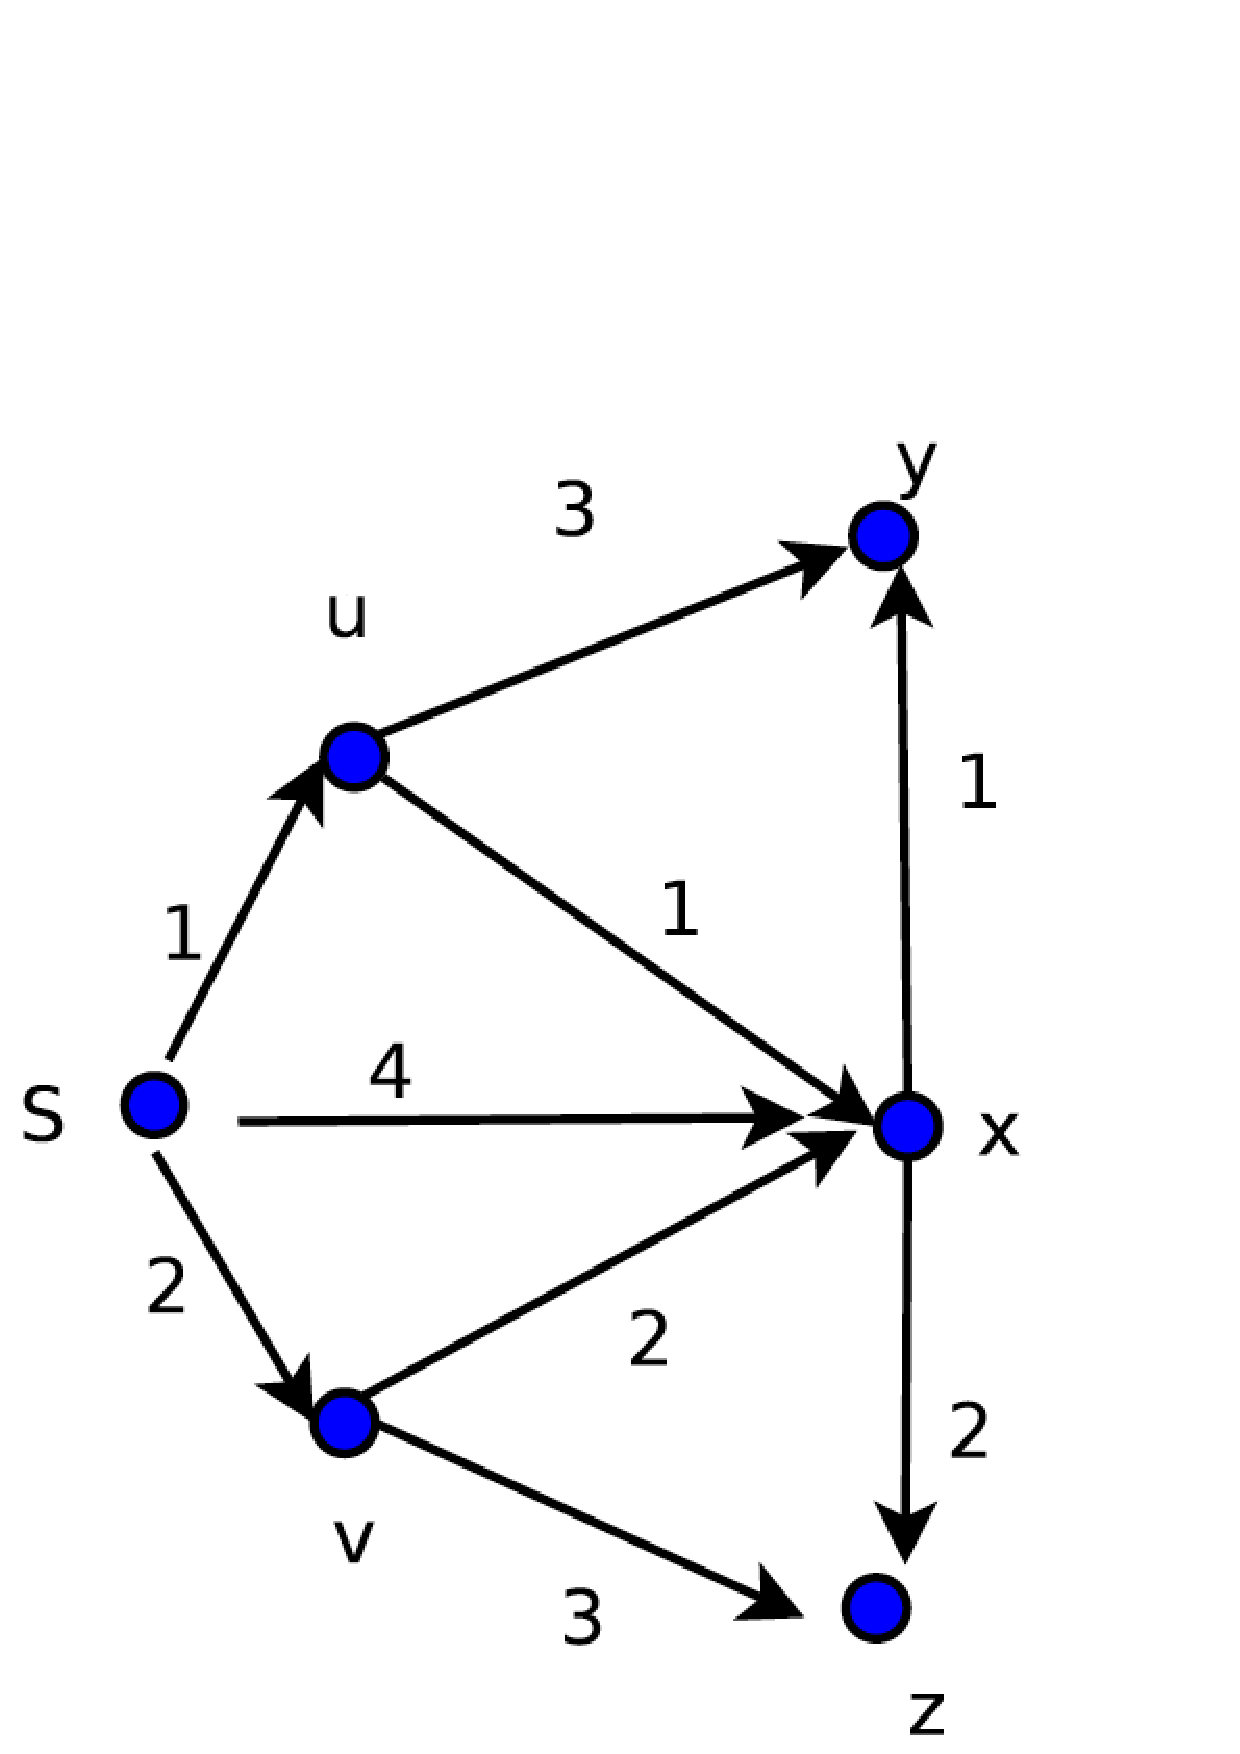
\includegraphics[width=0.9\textwidth]{L7-shortestpathexample.png}
 
\begin{tikzpicture}[auto,swap,scale=0.65]
% 
%    \foreach \pos/\name in {{(0,0)/s}, {(2,2)/u}, {(2,-2)/v}, {(5,0)/x}, {(5,-3)/z}, {(5,3)/y}}
%        \node[vertex,fill=blue!20] (\name) at \pos {$\name$};
%        
%        
%    \foreach \source/\dest/\weight in {s/u/1, s/v/2, s/x/4,   u/y/3,  u/x/1, x/y/1, v/x/2, v/z/3, x/z/2 } 
%            \path[edge] (\source) -- node[weight] {\tiny $\weight$} (\dest);
%	
%\end{tikzpicture} 
%		

  	\def\dx{-6};
 	\def\dy{-1.25};	
    \foreach \pos/\name in {{(0+\dx,0+\dy)/s}, {(2+\dx,1.4+\dy)/u}, {(2+\dx,-1.4+\dy)/v}, {(4+\dx,0+\dy)/x}, {(4+\dx,-2.5+\dy)/t}, {(4+\dx,2.5+\dy)/y}}
        \node[middlevertex,fill=blue!20] (\name) at \pos {$\name$};
        
        
    \foreach \source/\dest/\weight in {s/u/1, s/v/2, s/x/4,   u/y/3,  u/x/1, x/y/1, v/x/2, v/t/3, x/t/2 } 
            \path[edge] (\source) -- node[weight] {\tiny $\weight$} (\dest);
	
 
% \end{minipage}
% \begin{minipage}{0.45\textwidth}

%  \includegraphics[width=\textwidth]{L7-Dijkstraexample.png}
 
 %\begin{tikzpicture}[scale=0.8, auto,swap]
  
  	\def\d{0.7};
	
	%draw index 
 \def\dy{1};
 \def\dx{0};

    \foreach \i/\num/\name in { 1/k=0/, 2/1/s1,3/2/s2,4/3/s3,5/4/s4,6/5/}{
           \node[blue,thick] (\name) at (\i*\d+\d/2 + \dx*\d - \d, \d/2 + \dy * \d) {\tt \num};
    }

 \def\dy{0};
 \def\dx{0};
    \foreach \i/\num/\name in { 1/s/s1,2/u/s2,3/v/s3,4/x/s4, 5/y/,6/t/}{
         \node[blue,thick] (\name) at ( -1*\d+\d/2,  0.0 - \i*\d + \d/2 - \dy * \d + \d){$\num$};
    }

    
%score	
 \def\dy{0};
 \def\dx{0};
    \foreach \i/\num/\name in { 0/0/,1/0/S1,2/0/S2,3/0/,4/0/,5/0/}{
             \draw[  thick ] (\i*\d + \dx*\d,  0+ \dy*\d) rectangle (\i*\d+\d + \dx*\d, \d + \dy*\d);
         \node (\name) at (\i*\d+\d/2 + \dx*\d, \d/2 + \dy*\d) {\tiny $\num$};
    }



%   \draw[blue,ultra thick] (S1) circle[radius=\d/2];
%   \draw[blue,ultra thick] (S2) circle[radius=\d/2];
%   \draw[blue,ultra thick] (L) circle[radius=\d/2];
%
    
       
 \def\dy{-1};
 \def\dx{0};
    \foreach \i/\num/\name in { 0/-/,1/1/S1,2/1/,3/1/S3,4/1/,5/1/}{
             \draw[  thick ] (\i*\d + \dx*\d,  0+ \dy*\d) rectangle (\i*\d+\d + \dx*\d, \d + \dy*\d);
         \node (\name) at (\i*\d+\d/2 + \dx*\d, \d/2 + \dy*\d) {\tiny $\num$};
    }
 
      \draw[red,ultra thick] (S1) circle[radius=\d/2];
   
    
 \def\dy{-2};
 \def\dx{0};
    \foreach \i/\num/\name in { 0/-/,1/2/,2/2/S1,3/2/S3,4/2/,5/2/}{
             \draw[  thick ] (\i*\d + \dx*\d,  0+ \dy*\d) rectangle (\i*\d+\d + \dx*\d, \d + \dy*\d);
         \node (\name) at (\i*\d+\d/2 + \dx*\d, \d/2 + \dy*\d) {\tiny $\num$};
    }
       \draw[red,ultra thick] (S1) circle[radius=\d/2];
 
    
  \def\dy{-3};
 \def\dx{0};
    \foreach \i/\num/\name in { 0/-/,1/4/,2/2/S1,3/2/S3,4/2/,5/2/}{
             \draw[  thick ] (\i*\d + \dx*\d,  0+ \dy*\d) rectangle (\i*\d+\d + \dx*\d, \d + \dy*\d);
         \node (\name) at (\i*\d+\d/2 + \dx*\d, \d/2 + \dy*\d) {\tiny $\num$};
    }
       \draw[red,ultra thick] (S1) circle[radius=\d/2];
  
  \def\dy{-4};
 \def\dx{0};
    \foreach \i/\num/\name in { 0/-/,1/-/,2/4/,3/3/S1,4/3/,5/3/}{
             \draw[  thick ] (\i*\d + \dx*\d,  0+ \dy*\d) rectangle (\i*\d+\d + \dx*\d, \d + \dy*\d);
         \node (\name) at (\i*\d+\d/2 + \dx*\d, \d/2 + \dy*\d) {\tiny $\num$};
    }
         \draw[red,ultra thick] (S1) circle[radius=\d/2];

  \def\dy{-5};
 \def\dx{0};
    \foreach \i/\num/\name in { 0/-/,1/-/,2/5/,3/4/S3,4/4/S1,5/4/}{
             \draw[  thick ] (\i*\d + \dx*\d,  0+ \dy*\d) rectangle (\i*\d+\d + \dx*\d, \d + \dy*\d);
         \node (\name) at (\i*\d+\d/2 + \dx*\d, \d/2 + \dy*\d) {\tiny $\num$};
    }
        \draw[red,ultra thick] (S1) circle[radius=\d/2];
 


%draw blue rectangles 

 \def\dy{-1};
 \def\dx{0};
    \foreach \i/\num/\name in { 2/1/,3/1/S3,4/1/,5/1/}{
             \draw[  thick, green ] (\i*\d + \dx*\d,  0+ \dy*\d) rectangle (\i*\d+\d + \dx*\d, \d + \dy*\d);
    }
 
     
    
 \def\dy{-2};
 \def\dx{0};
    \foreach \i/\num/\name in { 3/2/S3,4/2/,5/2/}{
             \draw[  thick, green  ] (\i*\d + \dx*\d,  0+ \dy*\d) rectangle (\i*\d+\d + \dx*\d, \d + \dy*\d);
      }
 
    
  \def\dy{-3};
 \def\dx{0};
    \foreach \i/\num/\name in { 3/2/S3,4/2/,5/2/}{
             \draw[  thick, green ] (\i*\d + \dx*\d,  0+ \dy*\d) rectangle (\i*\d+\d + \dx*\d, \d + \dy*\d);
    }
 
   \def\dy{-4};
 \def\dx{0};
    \foreach \i/\num/\name in { 4/3/,5/3/}{
             \draw[  thick, green ] (\i*\d + \dx*\d,  0+ \dy*\d) rectangle (\i*\d+\d + \dx*\d, \d + \dy*\d);
    }
 
  \def\dy{-5};
 \def\dx{0};
    \foreach \i/\num/\name in {5/4/}{
             \draw[  thick, green ] (\i*\d + \dx*\d,  0+ \dy*\d) rectangle (\i*\d+\d + \dx*\d, \d + \dy*\d);
     }

\end{tikzpicture} 
 
% \end{minipage}
\end{figure}

\begin{itemize}
\item  Intuitively $v^*$ (in red circles) can be treated as \textcolor{red}{\bf has already been explored using at most $(k-1)$ edges}, and the distance will not change afterwards.
  Thus, the calculations of $OPT(v^*, k)$ (in green rectangles) are in fact redundant.
\item In other words, it suffices to calculate \begin{small} $OPT[v, k] = \min \begin{cases}
			OPT[v, k-1], \\
			\min_{<u,v>\in E} \{OPT[ u, k-1 ] + d(u,v) \} 
		\end{cases}$
		\end{small} for the \textcolor{red}{\bf unexplored nodes} $v \neq v^*$ at each step. 
\end{itemize}
}

\frame{
\frametitle{A faster implementation of {\sc Bellman\_Ford}}

{\sc Fast\_Bellman\_Ford}$( G, s, t )$
\begin{algorithmic}[1]
\STATE $S=\{s\}$; //$S$ denotes the set of explored nodes,
\FOR{$i=0$ to $n$ }
	\STATE $OPT[s, i] = 0;$
\ENDFOR
\FORALL{node $v \in V$ }
	\STATE $OPT[v, 0] = \infty;$
\ENDFOR 
\FOR{$k=1$ to $n-1$ }
	\FORALL{node \textcolor{red}{$v \notin S$} (in an arbitrary order) }
		\STATE \begin{footnotesize} $OPT[v, k] = \min \begin{cases}
			OPT[v, k-1], \\
			\min_{<u,v>\in E} \{OPT[ u, k-1 ] + d(u,v) \} 
			\end{cases}$
			\end{footnotesize}
	\ENDFOR
	\STATE{\textcolor{red}{Add the nodes with minimum $OPT(v, k)$ to $S$;}}
\ENDFOR
\RETURN{$OPT[ t, n-1]$};
\end{algorithmic}
}



\frame{
	\frametitle{Greedy-selection rule: select the nearest neighbor of $S$} 
	\begin{itemize}
		\item Now the question is how to efficiently calculate $OPT( v, k )$ for the \textcolor{red}{\bf unexplored nodes} $v \notin S$. Take the example shown below. The unexplored nodes include $v$, $x$, $y$ and $t$. 

\begin{figure}
% \begin{minipage}{0.40\textwidth}
%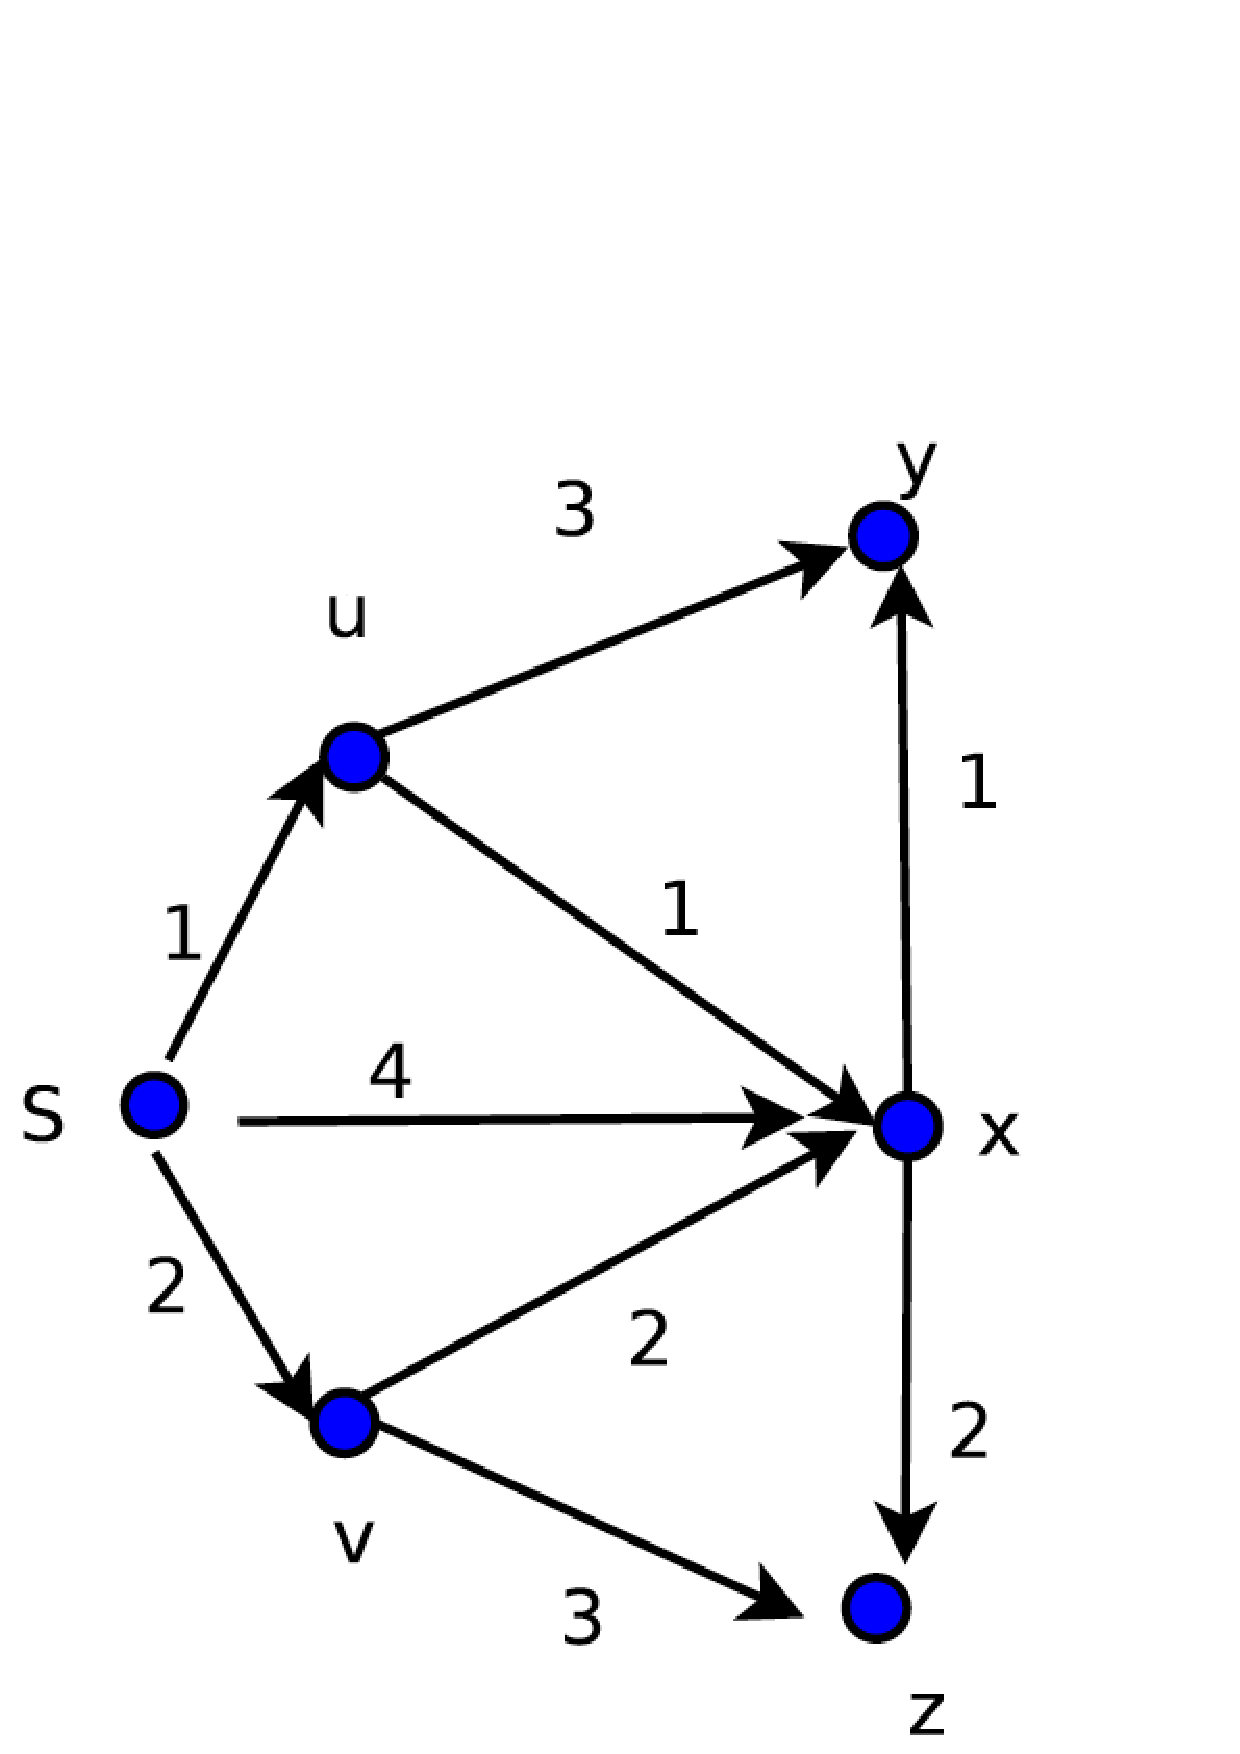
\includegraphics[width=0.9\textwidth]{L7-shortestpathexample.png}
 
\begin{tikzpicture}[auto,swap,scale=0.65]
% 
%    \foreach \pos/\name in {{(0,0)/s}, {(2,2)/u}, {(2,-2)/v}, {(5,0)/x}, {(5,-3)/z}, {(5,3)/y}}
%        \node[vertex,fill=blue!20] (\name) at \pos {$\name$};
%        
%        
%    \foreach \source/\dest/\weight in {s/u/1, s/v/2, s/x/4,   u/y/3,  u/x/1, x/y/1, v/x/2, v/z/3, x/z/2 } 
%            \path[edge] (\source) -- node[weight] {\tiny $\weight$} (\dest);
%	
%\end{tikzpicture} 
%		

  	\def\dx{-6};
 	\def\dy{-1.25};	
    \foreach \pos/\name in {{(0+\dx,0+\dy)/s}, {(2+\dx,1.4+\dy)/u}, {(2+\dx,-1.4+\dy)/v}, {(4+\dx,0+\dy)/x}, {(4+\dx,-2.5+\dy)/t}, {(4+\dx,2.5+\dy)/y}}
        \node[middlevertex,fill=blue!20] (\name) at \pos {$\name$};
        
        
    \foreach \source/\dest/\weight in {s/u/1, s/v/2, s/x/4,   u/y/3,  u/x/1, x/y/1, v/x/2, v/t/3, x/t/2 } 
            \path[edge] (\source) -- node[weight] {\tiny $\weight$} (\dest);
	
 
% \end{minipage}
% \begin{minipage}{0.45\textwidth}

%  \includegraphics[width=\textwidth]{L7-Dijkstraexample.png}
 
 %\begin{tikzpicture}[scale=0.8, auto,swap]
  
  	\def\d{0.7};
	
	%draw index 
 \def\dy{1};
 \def\dx{0};

    \foreach \i/\num/\name in { 1/k=0/, 2/1/s1,3/2/s2,4/3/s3,5/4/s4,6/5/}{
           \node[blue,thick] (\name) at (\i*\d+\d/2 + \dx*\d - \d, \d/2 + \dy * \d) {\tt \num};
    }

 \def\dy{0};
 \def\dx{0};
    \foreach \i/\num/\name in { 1/s/s1,2/u/s2,3/v/s3,4/x/s4, 5/y/,6/t/}{
         \node[blue,thick] (\name) at ( -1*\d+\d/2,  0.0 - \i*\d + \d/2 - \dy * \d + \d){$\num$};
    }

    
%score	
 \def\dy{0};
 \def\dx{0};
    \foreach \i/\num/\name in { 0/0/,1/0/S1,2/0/S2,3/0/,4/0/,5/0/}{
             \draw[  thick ] (\i*\d + \dx*\d,  0+ \dy*\d) rectangle (\i*\d+\d + \dx*\d, \d + \dy*\d);
         \node (\name) at (\i*\d+\d/2 + \dx*\d, \d/2 + \dy*\d) {\tiny $\num$};
    }



%   \draw[blue,ultra thick] (S1) circle[radius=\d/2];
%   \draw[blue,ultra thick] (S2) circle[radius=\d/2];
%   \draw[blue,ultra thick] (L) circle[radius=\d/2];
%
    
       
 \def\dy{-1};
 \def\dx{0};
    \foreach \i/\num/\name in { 0/-/,1/1/S1,2/1/,3/1/S3,4/1/,5/1/}{
             \draw[  thick ] (\i*\d + \dx*\d,  0+ \dy*\d) rectangle (\i*\d+\d + \dx*\d, \d + \dy*\d);
         \node (\name) at (\i*\d+\d/2 + \dx*\d, \d/2 + \dy*\d) {\tiny $\num$};
    }
 
      \draw[red,ultra thick] (S1) circle[radius=\d/2];
   
    
 \def\dy{-2};
 \def\dx{0};
    \foreach \i/\num/\name in { 0/-/,1/2/,2//S1,3//S3,4//,5//}{
             \draw[  thick ] (\i*\d + \dx*\d,  0+ \dy*\d) rectangle (\i*\d+\d + \dx*\d, \d + \dy*\d);
         \node (\name) at (\i*\d+\d/2 + \dx*\d, \d/2 + \dy*\d) {\tiny $\num$};
    }
%       \draw[red,ultra thick] (S1) circle[radius=\d/2];
 
    
  \def\dy{-3};
 \def\dx{0};
    \foreach \i/\num/\name in { 0/-/,1/4/,2//S1,3//S3,4//,5//}{
             \draw[  thick ] (\i*\d + \dx*\d,  0+ \dy*\d) rectangle (\i*\d+\d + \dx*\d, \d + \dy*\d);
         \node (\name) at (\i*\d+\d/2 + \dx*\d, \d/2 + \dy*\d) {\tiny $\num$};
    }
%       \draw[red,ultra thick] (S1) circle[radius=\d/2];
  
  \def\dy{-4};
 \def\dx{0};
    \foreach \i/\num/\name in { 0/-/,1/-/,2//,3//S1,4//,5//}{
             \draw[  thick ] (\i*\d + \dx*\d,  0+ \dy*\d) rectangle (\i*\d+\d + \dx*\d, \d + \dy*\d);
         \node (\name) at (\i*\d+\d/2 + \dx*\d, \d/2 + \dy*\d) {\tiny $\num$};
    }
%         \draw[red,ultra thick] (S1) circle[radius=\d/2];

  \def\dy{-5};
 \def\dx{0};
    \foreach \i/\num/\name in { 0/-/,1/-/,2//,3//S3,4//S1,5//}{
             \draw[  thick ] (\i*\d + \dx*\d,  0+ \dy*\d) rectangle (\i*\d+\d + \dx*\d, \d + \dy*\d);
         \node (\name) at (\i*\d+\d/2 + \dx*\d, \d/2 + \dy*\d) {\tiny $\num$};
    }
%        \draw[red,ultra thick] (S1) circle[radius=\d/2];
 


%draw blue rectangles 

 \def\dy{-1};
 \def\dx{0};
    \foreach \i/\num/\name in { 2/1/,3/1/S3,4/1/,5/1/}{
             \draw[  thick, green ] (\i*\d + \dx*\d,  0+ \dy*\d) rectangle (\i*\d+\d + \dx*\d, \d + \dy*\d);
    }
 
     
    
% \def\dy{-2};
% \def\dx{0};
%    \foreach \i/\num/\name in { 3/2/S3,4/2/,5/2/}{
%             \draw[  thick, green  ] (\i*\d + \dx*\d,  0+ \dy*\d) rectangle (\i*\d+\d + \dx*\d, \d + \dy*\d);
%      }
% 
%    
%  \def\dy{-3};
% \def\dx{0};
%    \foreach \i/\num/\name in { 3/2/S3,4/2/,5/2/}{
%             \draw[  thick, green ] (\i*\d + \dx*\d,  0+ \dy*\d) rectangle (\i*\d+\d + \dx*\d, \d + \dy*\d);
%    }
% 
%   \def\dy{-4};
% \def\dx{0};
%    \foreach \i/\num/\name in { 4/3/,5/3/}{
%             \draw[  thick, green ] (\i*\d + \dx*\d,  0+ \dy*\d) rectangle (\i*\d+\d + \dx*\d, \d + \dy*\d);
%    }
% 
%  \def\dy{-5};
% \def\dx{0};
%    \foreach \i/\num/\name in {5/4/}{
%             \draw[  thick, green ] (\i*\d + \dx*\d,  0+ \dy*\d) rectangle (\i*\d+\d + \dx*\d, \d + \dy*\d);
%     }

\end{tikzpicture} 
 
% \end{minipage}
\end{figure}
%	\item Take the example shown above: It suffices to consider nodes $v$, $x$, and $y$ as they are adjacent to explored nodes ($s$ and $u$) and it is  unnecessary to consider node $t$ as it is not adjacent to explored nodes. Among these nodes, $v$ and $x$ are the nearest nodes, and thus have their distance determined. 

%		 \item Recall that the collection of the shortest paths from $s$ to all nodes $v \in V$ form a shortest path tree. To construct the shortest path tree, we start from the node $s$ and select the nearest unexplored node at each step. 

		\item Note that it is unnecessary to consider all unexplored nodes; instead, we can consider \textcolor{red}{\bf only the unexplored nodes adjacent to an explored node}, i.e., nodes $v, x, y$. Furthermore, among these nodes, \textcolor{red}{\bf the nearest ones ($v$ and $x$)} have their shortest distance determined. Thus we can iteratively select such nodes until reaching node $t$. 

	\end{itemize}
}



\frame{
%\frametitle{Greedy-selection property} 
\begin{footnotesize}
\begin{Theorem}
Let $S$ denote the \textcolor{blue}{\bf explored} nodes, and for each explored node $v$, let $d(v)$ denote the shortest distance from $s$ to $v$. \textcolor{red}{\bf Consider the nearest unexplored node $u^*$ adjacent to an explored node}, i.e., $u^*$ is the node $u$ ($u \notin S$) that minimizes $d'(u)=\min_{w\in S}\{d(w)+d(w, u)\}$. Then the path $P=s\rightarrow...\rightarrow w \rightarrow u^*$  is one of the shortest paths from $s$ to $u^*$ with distance $d'(u^*)$. 
\end{Theorem}
\begin{Proof} 
\begin{itemize}
\begin{footnotesize}
 	\item Consider another path $P'$ from $s$ to $u^*$:  $P'= s \rightarrow...\rightarrow x \rightarrow y \rightarrow...\rightarrow u^*$. Let  $y$ denote the first node in $P'$ leaving out of $S$. 
 	\item We decompose $P'$ into two parts: $s \rightarrow...\rightarrow x \rightarrow y$, and $y\rightarrow...\rightarrow u^*$. 
 	\item The first part should be longer. Thus,  $ |P'|  \geq   d(s, x) + d(x, y)    \geq   d'(u^*)$.  
%\begin{figure}
%	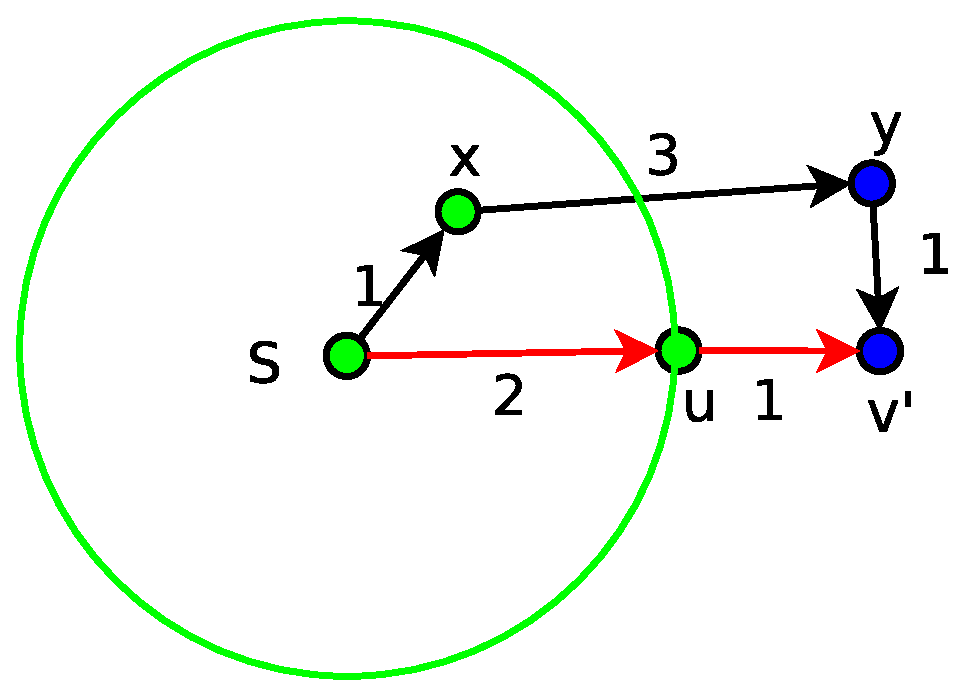
\includegraphics[width=1.5in]{L7-Dijkstraalgoalgoproof.eps}
%\end{figure}
\begin{figure}
\begin{tikzpicture}[scale=0.9, auto,swap]
 
   \draw[fill=gray!20, draw=white] (0,0) circle[radius=2];

    \foreach \pos/\name in {{(0,0)/s}, {(2,0)/w}, {(0, 1)/x}, {(3,1)/y}, {(4,1)/z}, {(3,0)/u^*}}
        \node[middlevertex,fill=blue!20] (\name) at \pos {$\name$};
        
        
    \foreach \source/\dest/\weight in {s/w/2, s/x/1, x/y/3,   y/u^*/1, y/z/1, w/u^*/1 } 
            \path[edge] (\source) -- node{\small $\weight$} (\dest);

        
    \foreach \source/\dest/\weight in {s/w/2,  w/u^*/1 } 
            \path[edge, red] (\source) -- node{\small $\weight$} (\dest);

   \node[red, ultra thick] at (0,-1) {$S: $ explored nodes}; 	
		
\end{tikzpicture} 
\end{figure}   
\end{footnotesize}
\end{itemize}
\end{Proof}
\end{footnotesize}
}


\frame{
	\frametitle{{\sc Bellman\_Ford} vs {\sc Dijkstra}: two differences} 
	\begin{enumerate}
		\item  {\footnotesize Let $v^*$ denote the nearest node from  $s$ using at most $k-1$ edges.  The shortest distance $d(v^*)$ will not change afterwards. } 

\begin{figure}
% \begin{minipage}{0.40\textwidth}
%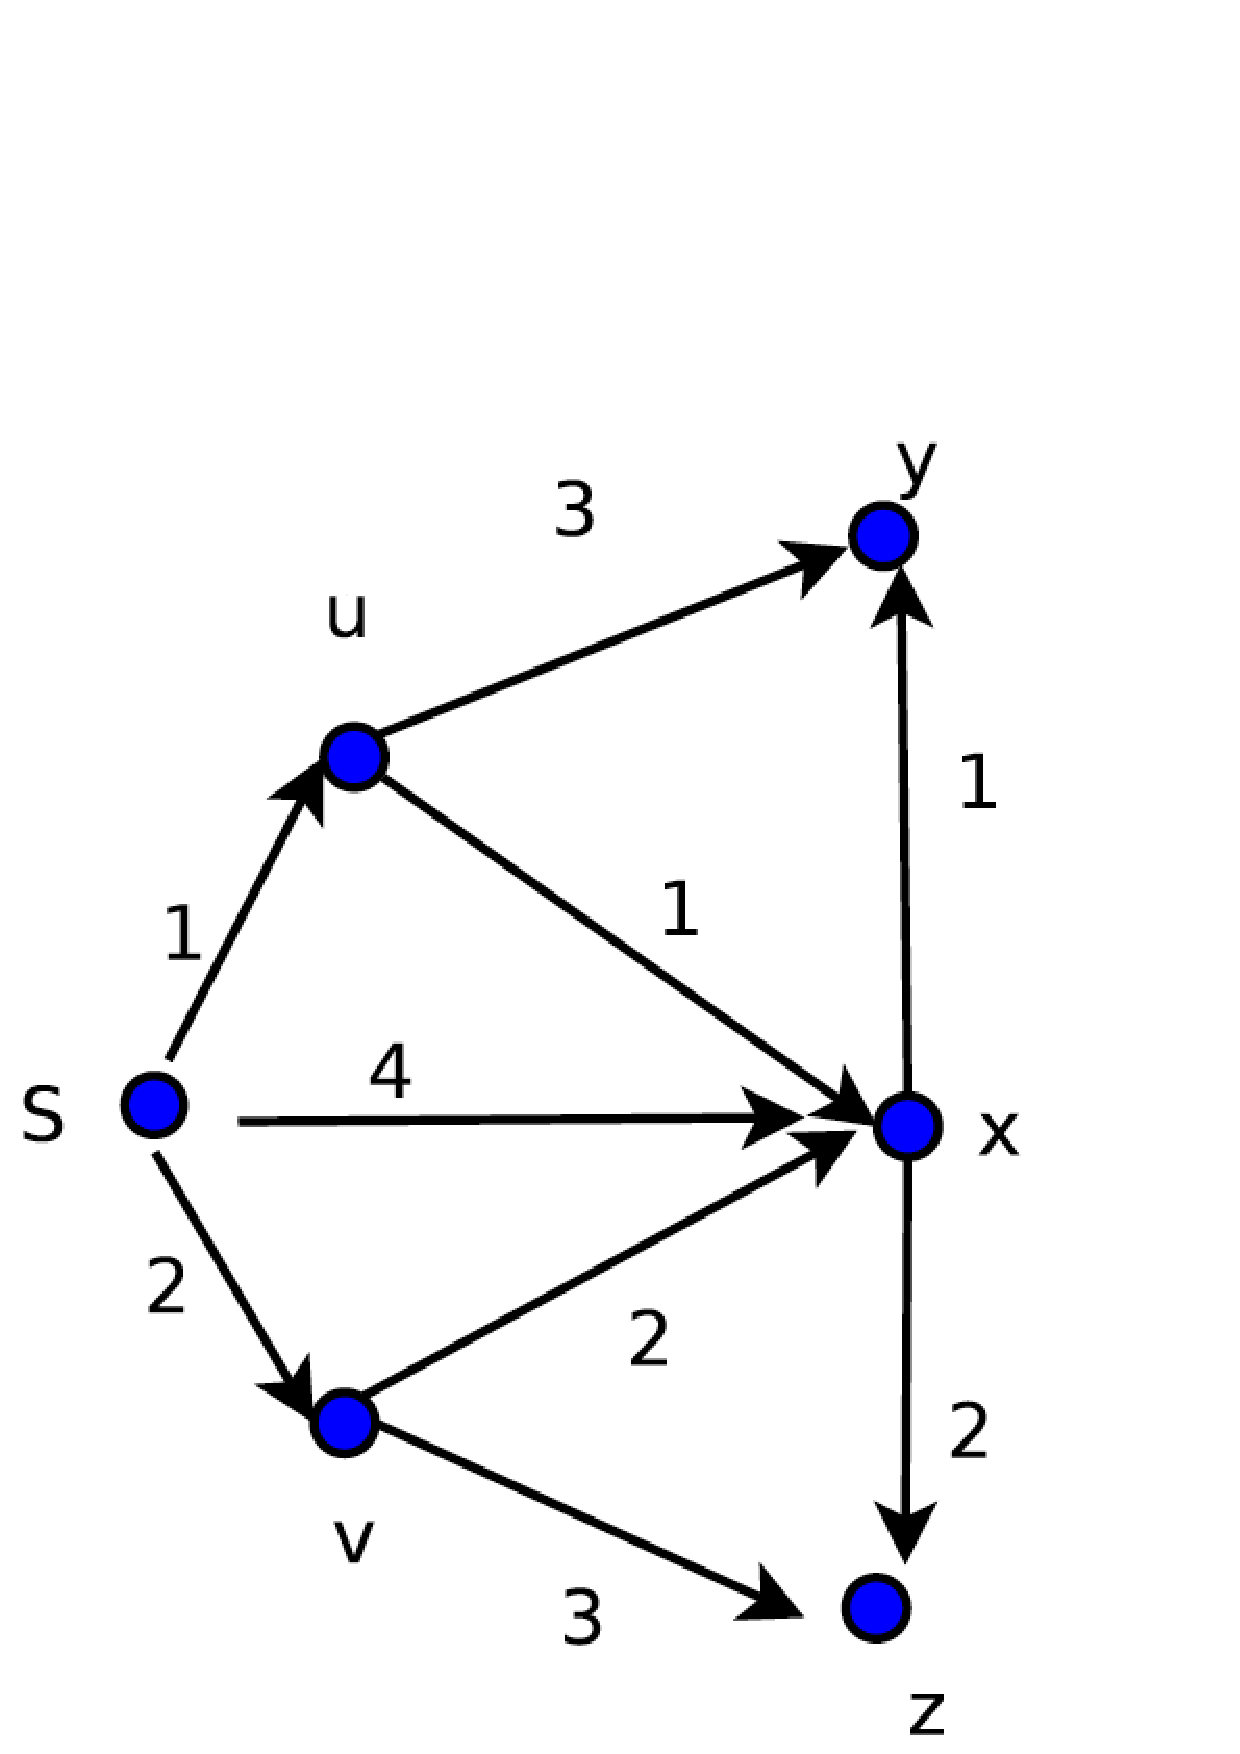
\includegraphics[width=0.9\textwidth]{L7-shortestpathexample.png}
 
\begin{tikzpicture}[auto,swap,scale=0.65]
% 
%    \foreach \pos/\name in {{(0,0)/s}, {(2,2)/u}, {(2,-2)/v}, {(5,0)/x}, {(5,-3)/z}, {(5,3)/y}}
%        \node[vertex,fill=blue!20] (\name) at \pos {$\name$};
%        
%        
%    \foreach \source/\dest/\weight in {s/u/1, s/v/2, s/x/4,   u/y/3,  u/x/1, x/y/1, v/x/2, v/z/3, x/z/2 } 
%            \path[edge] (\source) -- node[weight] {\tiny $\weight$} (\dest);
%	
%\end{tikzpicture} 
%		

  	\def\dx{-6};
 	\def\dy{-1.25};	
    \foreach \pos/\name in {{(0+\dx,0+\dy)/s}, {(2+\dx,1.4+\dy)/u}, {(2+\dx,-1.4+\dy)/v}, {(4+\dx,0+\dy)/x}, {(4+\dx,-2.5+\dy)/t}, {(4+\dx,2.5+\dy)/y}}
        \node[middlevertex,fill=blue!20] (\name) at \pos {$\name$};
        
        
    \foreach \source/\dest/\weight in {s/u/1, s/v/2, s/x/4,   u/y/3,  u/x/1, x/y/1, v/x/2, v/t/3, x/t/2 } 
            \path[edge] (\source) -- node[weight] {\tiny $\weight$} (\dest);
	
 
% \end{minipage}
% \begin{minipage}{0.45\textwidth}

%  \includegraphics[width=\textwidth]{L7-Dijkstraexample.png}
 
 %\begin{tikzpicture}[scale=0.8, auto,swap]
  
  	\def\d{0.7};
	
	%draw index 
 \def\dy{1};
 \def\dx{0};

    \foreach \i/\num/\name in { 1/k=0/, 2/1/s1,3/2/s2,4/3/s3,5/4/s4,6/5/}{
           \node[blue,thick] (\name) at (\i*\d+\d/2 + \dx*\d - \d, \d/2 + \dy * \d) {\tt \num};
    }

 \def\dy{0};
 \def\dx{0};
    \foreach \i/\num/\name in { 1/s/s1,2/u/s2,3/v/s3,4/x/s4, 5/y/,6/t/}{
         \node[blue,thick] (\name) at ( -1*\d+\d/2,  0.0 - \i*\d + \d/2 - \dy * \d + \d){$\num$};
    }

    
%score	
 \def\dy{0};
 \def\dx{0};
    \foreach \i/\num/\name in { 0/0/,1/0/S1,2/0/S2,3/0/,4/0/,5/0/}{
             \draw[  thick ] (\i*\d + \dx*\d,  0+ \dy*\d) rectangle (\i*\d+\d + \dx*\d, \d + \dy*\d);
         \node (\name) at (\i*\d+\d/2 + \dx*\d, \d/2 + \dy*\d) {\tiny $\num$};
    }



%   \draw[blue,ultra thick] (S1) circle[radius=\d/2];
%   \draw[blue,ultra thick] (S2) circle[radius=\d/2];
%   \draw[blue,ultra thick] (L) circle[radius=\d/2];
%
    
       
 \def\dy{-1};
 \def\dx{0};
    \foreach \i/\num/\name in { 0/-/,1/1/S1,2/1/,3/1/S3,4/1/,5/1/}{
             \draw[  thick ] (\i*\d + \dx*\d,  0+ \dy*\d) rectangle (\i*\d+\d + \dx*\d, \d + \dy*\d);
         \node (\name) at (\i*\d+\d/2 + \dx*\d, \d/2 + \dy*\d) {\tiny $\num$};
    }
 
      \draw[red,ultra thick] (S1) circle[radius=\d/2];
   
    
 \def\dy{-2};
 \def\dx{0};
    \foreach \i/\num/\name in { 0/-/,1/2/,2//S1,3//S3,4//,5//}{
             \draw[  thick ] (\i*\d + \dx*\d,  0+ \dy*\d) rectangle (\i*\d+\d + \dx*\d, \d + \dy*\d);
         \node (\name) at (\i*\d+\d/2 + \dx*\d, \d/2 + \dy*\d) {\tiny $\num$};
    }
%       \draw[red,ultra thick] (S1) circle[radius=\d/2];
 
    
  \def\dy{-3};
 \def\dx{0};
    \foreach \i/\num/\name in { 0/-/,1/4/,2//S1,3//S3,4//,5//}{
             \draw[  thick ] (\i*\d + \dx*\d,  0+ \dy*\d) rectangle (\i*\d+\d + \dx*\d, \d + \dy*\d);
         \node (\name) at (\i*\d+\d/2 + \dx*\d, \d/2 + \dy*\d) {\tiny $\num$};
    }
%       \draw[red,ultra thick] (S1) circle[radius=\d/2];
  
  \def\dy{-4};
 \def\dx{0};
    \foreach \i/\num/\name in { 0/-/,1/-/,2//,3//S1,4//,5//}{
             \draw[  thick ] (\i*\d + \dx*\d,  0+ \dy*\d) rectangle (\i*\d+\d + \dx*\d, \d + \dy*\d);
         \node (\name) at (\i*\d+\d/2 + \dx*\d, \d/2 + \dy*\d) {\tiny $\num$};
    }
%         \draw[red,ultra thick] (S1) circle[radius=\d/2];

  \def\dy{-5};
 \def\dx{0};
    \foreach \i/\num/\name in { 0/-/,1/-/,2//,3//S3,4//S1,5//}{
             \draw[  thick ] (\i*\d + \dx*\d,  0+ \dy*\d) rectangle (\i*\d+\d + \dx*\d, \d + \dy*\d);
         \node (\name) at (\i*\d+\d/2 + \dx*\d, \d/2 + \dy*\d) {\tiny $\num$};
    }
%        \draw[red,ultra thick] (S1) circle[radius=\d/2];
 


%draw blue rectangles 

 \def\dy{-1};
 \def\dx{0};
    \foreach \i/\num/\name in { 2/1/,3/1/S3,4/1/,5/1/}{
             \draw[  thick, green ] (\i*\d + \dx*\d,  0+ \dy*\d) rectangle (\i*\d+\d + \dx*\d, \d + \dy*\d);
    }
 
     
    
% \def\dy{-2};
% \def\dx{0};
%    \foreach \i/\num/\name in { 3/2/S3,4/2/,5/2/}{
%             \draw[  thick, green  ] (\i*\d + \dx*\d,  0+ \dy*\d) rectangle (\i*\d+\d + \dx*\d, \d + \dy*\d);
%      }
% 
%    
%  \def\dy{-3};
% \def\dx{0};
%    \foreach \i/\num/\name in { 3/2/S3,4/2/,5/2/}{
%             \draw[  thick, green ] (\i*\d + \dx*\d,  0+ \dy*\d) rectangle (\i*\d+\d + \dx*\d, \d + \dy*\d);
%    }
% 
%   \def\dy{-4};
% \def\dx{0};
%    \foreach \i/\num/\name in { 4/3/,5/3/}{
%             \draw[  thick, green ] (\i*\d + \dx*\d,  0+ \dy*\d) rectangle (\i*\d+\d + \dx*\d, \d + \dy*\d);
%    }
% 
%  \def\dy{-5};
% \def\dx{0};
%    \foreach \i/\num/\name in {5/4/}{
%             \draw[  thick, green ] (\i*\d + \dx*\d,  0+ \dy*\d) rectangle (\i*\d+\d + \dx*\d, \d + \dy*\d);
%     }

\end{tikzpicture} 
 
% \end{minipage}
\end{figure}
		
		\item {\footnotesize Let's $u^*$ denote the nearest unexplored node adjacent to an explored node. The shortest path from $s$ to  $u^*$ is determined.  }
\begin{figure}
\begin{tikzpicture}[scale=0.8, auto,swap]
 
   \draw[fill=gray!20, draw=white] (0,0) circle[radius=2];

    \foreach \pos/\name in {{(0,0)/s}, {(2,0)/w}, {(0, 1)/x}, {(3,1)/y}, {(4,1)/z}, {(3,0)/u^*}}
        \node[middlevertex,fill=blue!20] (\name) at \pos {$\name$};
        
        
    \foreach \source/\dest/\weight in {s/w/2, s/x/1, x/y/3,   y/u^*/1, y/z/1, w/u^*/1 } 
            \path[edge] (\source) -- node{\tiny $\weight$} (\dest);

        
    \foreach \source/\dest/\weight in {s/w/2,  w/u^*/1 } 
            \path[edge, red] (\source) -- node{\tiny $\weight$} (\dest);

   \node[red, ultra thick] at (0,-1) {$S: $ explored nodes}; 	
		
\end{tikzpicture} 
\end{figure}   

	\end{enumerate}

}

\frame{
\frametitle{Dijkstra's algorithm [1959] }
\begin{small}
{\sc Dijkstra}$(G, s, t )$
\begin{algorithmic}[1]
\STATE $d(s)=0$; //$d(u)$ stores upper bound of the shortest distance from $s$ to $u$;
\FORALL{node $v \neq s$}
	\STATE{$d(v) = +\infty$; } 
\ENDFOR
\STATE $S=\{ \}$; // Let $S$ be the set of explored nodes;
\WHILE{$S \neq V$}
	\STATE \textcolor{red}{Select the unexplored node $v^*$ ($v^* \notin S$) that minimizes $d(v)$;}
	\STATE $S=S \cup \{v^*\}$;
	\FORALL{unexplored node $v$  adjacent to an explored node}
		\STATE  $d(v)=\min\{d(v), \min_{u\in S}\{d(u)+d(u,v)\} \}$;
	\ENDFOR 
\ENDWHILE
\end{algorithmic}
\end{small} 
\begin{itemize}
	\begin{small} 
	\item Lines $(9-11)$ are called \textcolor{blue}{\bf ``relaxing"}. That is, we test whether the shortest-path to $v$ found so far can be improved by going through $u$, and if so, update $d(v)$. 
	\item When $d_{u,v} = 1$ for any edge $<u,v>$, the Dijkstra's algorithm 
reduces to BFS, and thus can be treated as \textcolor{red}{\bf weighted BFS}. 
\end{small} 
\end{itemize}

}








\frame{
\frametitle{Implementing Dijkstra's algorithm using priority queue }


\begin{small}
{\sc Dijkstra}$( G, s, t )$
\begin{algorithmic}[1]
\STATE $key(s) = 0;$  //$key(u)$ stores an upper bound of the shortest distance from $s$ to $u$;
\STATE $PQ.$ {\sc Insert} $(s)$;
\FORALL{node $v \neq s$ }
	\STATE $key(v) = +\infty $
	\STATE $PQ.$ {\sc Insert} $(v)$ \textcolor{red}{//$n$ times}
\ENDFOR
\STATE $S=\{ \}$; // Let $S$ be the set of explored nodes;
\WHILE{$S \neq V $}
	\STATE $v^*=PQ.$ {\sc ExtractMin}$()$; \textcolor{red}{//$n$ times}
	\STATE $S=S \cup \{v^*\}$;
	\FORALL{$v \notin S$ and $<v^*, v> \in E$}
		\IF{$key(v^*) + d(v^*, v) < key(v)$}
			\STATE $PQ.${\sc DecreaseKey}($v, key(v^*) + d(v^*, v)$); \textcolor{red}{//$m$ times}
		\ENDIF
	\ENDFOR
\ENDWHILE
\end{algorithmic}
\end{small}
Here $PQ$ denotes a min-priority queue. 
(see a demo)
}



\frame{
	\frametitle{Dijkstra's algorithm: a 20-minute invention without pencil and paper} 

\begin{small}
{\it 
	
	What is the shortest way to travel from Rotterdam to Groningen, in general: from given city to given city? It is the algorithm for the shortest path, which I designed in about twenty minutes. One morning I was shopping in Amsterdam with my young fiancée, and tired, we sat down on the café terrace to drink a cup of coffee and I was just thinking about whether I could do this, and I then designed the algorithm for the shortest path. As I said, it was a twenty-minute invention. In fact, it was published in ’59, three years late. The publication is still readable, it is, in fact, quite nice. One of the reasons that it is so nice was that I designed it without pencil and paper. I learned later that one of the advantages of designing without pencil and paper is that you are almost forced to avoid all avoidable complexities. Eventually that algorithm became, to my great amazement, one of the cornerstones of my fame.

All the programming I did was on paper. So I was quite
used to developing programs without testing them.

Thanks to
my isolation,
I would do things differently than people subjected to the standard pressures of conformity.
I was a free man.
} 
\end{small}
— Edsger Dijkstra, in an interview with Philip L. Frana, Communications of the ACM 53 (8), 2001.
}

\frame{
\frametitle{Contributions by Edsger W.  Dijkstra  }

\begin{figure}
 	 \includegraphics[width=1.1in]{Dijkstra.jpg}
\end{figure}
\begin{small} 
\begin{itemize} 
\item  The semaphore construct for coordinating multiple processors and programs. 
\item The concept  of self-stabilization --- an alternative way to ensure the reliability of the system
\item  "A Case against the GO TO Statement", regarded as a major step towards the widespread deprecation of the GOTO statement and its effective replacement by structured control constructs, such as the while loop.
\item ...
\end{itemize}
\end{small} 
} 


\frame{
\frametitle{{\sc ShortestPath}: Bellman-Ford algorithm vs. Dijkstra algorithm } 

\begin{itemize}
\item A slight change of edge weights leads to a significant change of algorithm design. 
\begin{enumerate}
\item No negative cycle: an optimal path from $s$ to $v$ has at most $n-1$ edges; thus the optimal solution is $OPT( v, n-1)$. To calculate $OPT(v, n-1 )$, we appeal to the following recursion: 

$OPT[v, k] = \min \begin{cases}
		OPT[ v, k-1], \\
		\min_{<u,v>\in E} \{OPT[u, k-1 ] + d(u,v) \} 
		\end{cases}$
\ \\		
\item No negative edge: This stronger constraint on edge weights implies greedy-selection property. In particular, it is unnecessary to calculate $OPT(v, i)$ for any explored node $v \in S$, and for the nearest unexplored node adjacent to an explored node, its shortest distance is determined. 
\end{enumerate}
\end{itemize}
} 


\frame{
 	\begin{block}{}
	Time complexity analysis
	\end{block} 
} 

\frame{
	\frametitle{Time complexity of the Dijkstra's algorithm} 

  \begin{table}
  \begin{tabular}{crrrr}
  \hline  \hline
  Operation & Linked  & Binary  & Binomial  & Fibonacci  \\
            &  list &  heap &  heap & heap \\
  \hline
  {\sc MakeHeap} & $ 1 $ &  $1$  & $ 1 $ & $1$  \\ 
  {\sc Insert} & $ 1 $ &  $\log n$  & $ \log n $ & $1$  \\ 
   {\sc ExtractMin} & $ n $ &  $\log n$  & $ \log n  $ & $ \log n $  \\ 
  {\sc DecreaseKey} & $ 1 $ &  $\log n$  & $ \log n $ & $1$  \\ 
  {\sc Delete} & $ n $ &  $\log n$  & $ \log n $ & $\log n$  \\ 
  {\sc Union} & $ 1 $ &  $ n $  & $ \log n $ & $1$  \\ 
   {\sc FindMin} & $ n $ &  $1$  & $ \log n $ & $1$  \\ 
  \hline 
  {\sc Dijkstra} & $ O(n^2) $ &  $ O(m \log n) $  & $ O( m \log n ) $ & $ O( m + n \log n) $  \\ 
  \hline \hline 
  \end{tabular} 
  \end{table}
The Dijkstra's algorithm: $n$ {\sc Insert}, $n$ {\sc ExtractMin}, and $m$ {\sc DecreaseKey}. 
}

\frame{
	\begin{block}{}
		Extension: can we reweigh the edges to make all weight positive?  
	\end{block}
}

\frame{
	\frametitle{Trial 1: Increasing all edge weights  by the same amount } 

\begin{figure}
\begin{tikzpicture}[scale=1., auto,swap]
    % Draw a 7,11 network
    % First we draw the vertices
    \foreach \pos/\name/\label in {{(0,0)/s/s}, {(1.5,0)/u/u}, {(1,1)/v/v}, {(2,1)/w/w}, {(3, 0)/t/t}}
            \node[smallvertex,draw=black, fill=blue!20] (\name) at \pos {\tiny $\label$};
  
    % Connect vertices with edges and draw weights
  \foreach \source/ \dest /\weight in {s/u/{1}, s/v/{-1}, v/w/{1}, w/t/{-1}, u/t/{1}}
        \draw[->] (\source) -- node[weight,above] {\tiny $\weight$} (\dest);
%       \draw[dashed, ->] (0,0) arc  (120:60:2);

  \foreach \source/ \dest /\weight in {s/v/{-1}, v/w/{1}, w/t/{-1}}
        \draw[->, red] (\source) -- node[weight,above] {} (\dest);

\draw[->, green, ultra thick] (3.8, 0.5) -- (4.3, 0.5); 

   % Draw a 7,11 network
    % First we draw the vertices
    \foreach \pos/\name/\label in {{(5,0)/s/s}, {(6.5,0)/u/u}, {(6,1)/v/v}, {(7,1)/w/w}, {(8, 0)/t/t}}
            \node[smallvertex,draw=black, fill=blue!20] (\name) at \pos {\tiny $\label$};
  
    % Connect vertices with edges and draw weights
  \foreach \source/ \dest /\weight in {s/u/{6}, s/v/{4}, v/w/{6}, w/t/{4}, u/t/{6}}
        \draw[->] (\source) -- node[weight,above] {\tiny $\weight$} (\dest);
%       \draw[dashed, ->] (0,0) arc  (120:60:2);

  \foreach \source/ \dest /\weight in {s/u/{-1}, u/t/{-1}}
        \draw[->, red] (\source) -- node[weight,above] {} (\dest);


   \end{tikzpicture}
\end{figure}

\begin{itemize}
\item Increasing all the weight by 5 changes the shortest path from $s$ to $t$.
\item Reason: Different paths might change by different amount although 	
all edges change by the same mount. 		
\end{itemize}

}

\frame{
	\frametitle{Trial 2: Increasing an edge weight according to its two ends}
\begin{itemize}
\item For different paths starting from  $u$ to $v$, 
one of the constraints of reweighing is to maintain the  order of these paths under the original weighting function. In other words, the change of  distance following a path is independent of the intermediate nodes of the path. Thus, for any path $u \leadsto v$, we represent the new distance as:  
\[
d'(u \leadsto v) = d( u \leadsto v) + c(u) - c(v)
\]
where $c(v)$ is a number associated with node $v$.  	 
\item As a special case, each edge $(u, v)$ is reweighed as follows.	
\[
d'(u, v) = d( u, v) + c(u) - c(v)
\]	 
\item Note another constraint is $d'(u, v) \geq 0$ for any edge $(u, v)$. How to achieve this objective? 
\end{itemize}
} 

\frame{
	\frametitle{Reweighing schema} 
	\begin{itemize}
		\item Basic idea: We first add a new node $s^*$ and connect it to each node $v$ with an edge weight $d( s^*, v) = 0$, $d( v, s^*) = \infty$. Next we set $c(v)$ as $dist(s^*, v)$, i.e., the shortest distance from $s^*$ to $v$. 
		\item We can prove that for any node pair $u$ and $v$, 		 
\[
	d'(u, v) = d(u, v) + dist( u) - dist( v) \geq 0
\] 
(Why? If $d'(u, v) < 0$, then $d(u, v) + dist( u) < dist( v)$, which is contradict to the fact that $dist(v)$ is the shortest distance to $v$.) 
	\end{itemize}
}	

\frame{
	\frametitle{Johnson algorithm for all pairs shortest path [1977]}

\begin{small}
{\sc Johnson}$( G )$
\begin{algorithmic}[1]
\STATE Create a new node $s^*$; 
\FORALL{node $v \neq s^*$} 
	\STATE{	$d(s^*, v) = 0$}
\ENDFOR
\STATE Run {\sc Bellman\_Ford} algorithm to calculate the shortest distance from $s^*$ to each node $v$ (denoted as $dist(s^*, v))$; 
\STATE Reweighting: 	$d'(u, v) = d(u, v) + dist( s^*, u) - dist(s^*, v) $ 
\FORALL{node $u \neq s^*$} 
	\STATE Run Dijkstra's algorithm with the new weight $d'$ to calculate the shortest paths from $u$ to each node $v$ (denoted as $d^*(u,v)$); 
	\FORALL{node $v \neq s^*$}
		\STATE $d^*( u, v) = d^*(u, v)  - dist( s^*, u) + dist( s^*, v);$ 
	\ENDFOR
\ENDFOR 
\RETURN{$d^*(u,v)$ for each node pair $(u, v)$;}
\end{algorithmic}
\end{small}
Time complexity: $O( mn + n^2 \log n)$. 	
	
} 


\frame{
	\begin{block}{}
		Extension: data structures designed to speed up the Dijkstra's algorithm
	\end{block}
}

\frame{
\frametitle{Binary heap, Binomial heap, and Fibonacci heap} 

\begin{figure}
 \begin{minipage}{0.30\textwidth}
     \includegraphics[width=0.8\textwidth]{Floyd.png}
 \end{minipage}
 \begin{minipage}{0.30\textwidth}
     \includegraphics[width=0.8\textwidth]{JeanVuillemin.png}
 \end{minipage}
 \begin{minipage}{0.30\textwidth}
     \includegraphics[width=0.8\textwidth]{Tarjan.png}
 \end{minipage}
 \caption{ Robert W. Floyd, Jean Vuillenmin, Robert Tarjan}
 \end{figure}

(See extra slides for binary heap, binomial heap and Fibonacci heap)
} 


\frame{
\begin{block}{}
{\sc Huffman Code} 
\end{block}
}


\frame{
\frametitle{Compressing files }

\begin{itemize} 
\item 
Practical problem: how to compact a file when you have the knowledge of frequency of letters? 
\item 
Example: 
\begin{footnotesize}
\begin{table}{
\begin{tabular}{lllllllll} 
\hline
SYMBOL & \texttt{A} & \texttt{B} & \texttt{C} & \texttt{D} & \texttt{E}  &\\ \hline
Frequency & 24 & 12 & 10 & 8 & 8 & \\ 
Fixed Length Code & \texttt{000} & \texttt{001} &\texttt{010} &\texttt{011} &\texttt{100} & $E(L)=186$ \\
Variable Length Code & \texttt{00} & \texttt{01} &\texttt{10} &\texttt{110} &\texttt{111}& $E(L)=140$ \\
\hline
\end{tabular} } {} 
\end{table} 
\end{footnotesize}
\end{itemize} 
}

\frame{
\frametitle{Formulation }

\begin{block}{}
 {\bf INPUT: } \\a set of symbols $S=\{s_1, s_2, ..., s_n\}$ with its appearance frequency $P=\{p_1, p_2, ..., p_n\}$; \\ 
 {\bf OUTPUT: } \\assign each symbol with a binary code $C_i$ to minimize the length expectation $\sum_i p_i | C_i |$.  
\end{block}
} 


\frame[allowframebreaks]{
\frametitle{Requirement: prefix code}

\begin{itemize}
 \item 
 To avoid the potential ambiguity in decoding, we require the coding to be {\bf prefix code}. 
 \begin{definition}[Prefix coding] 
A prefix coding for a symbol set $S$ is a coding such that for any symbols $x, y \in S$,  the code $C(x)$ is not prefix of the code $C(y)$. 
\end{definition}
\item
Intuition: A prefix code can be represented as a binary tree, where a leaf represents a symbol, and the path to a leaf represents the code. 
\item
Our objective: to design an optimal tree $T$ to minimize expected length $E(T)$ (the size of the compressed file). 
\end{itemize}

\begin{figure}
	\includegraphics[width=3.95in]{L7-prefixcode.eps}
\end{figure}
}

%\frame{ 
%\frametitle{We need a complete tree!}
%\begin{figure} 
% \includegraphics[width=4in]{binarytree.eps}
%\end{figure}
%} 

\frame{
\frametitle{Full binary tree}
\begin{Theorem}{}
 An optimal binary tree should be a full tree. 
\end{Theorem}
\begin{Proof}
\begin{itemize}
 \item 
 Suppose $T$ is an optimal tree but is not full; \\
\item There is a node $u$ with only one child $v$; \\
\item Construct a new tree $T'$, where $u$ is replaced with $v$; 
\item $E(T') \leq E(T)$ since any child of $v$ has a shorter code. 
\end{itemize}
\end{Proof}

\begin{figure}
	\includegraphics[width=2.2in]{L7-prefixcodefulltree.eps}
\end{figure}
}


\frame{
	\begin{block}{}
	But how to construct the optimal tree? \\ Let's describe the solving process as a multistage decision process. 
	\end{block} 	
}

\frame{
	\frametitle{A  top-down multiple-decision process} 
	
%	\begin{figure}
%\begin{tikzpicture}[scale=1., auto,swap]
%    % Draw a 7,11 network
%    % First we draw the vertices
%    \foreach \pos/\name/\label in {{(0,0)/root/}, 
%    {(-3,-1)/L/}, {(3,-1)/R/}}
%        \node[smallvertex,draw=black, fill=white!20] (\name) at \pos {};
%        
%        
%        \foreach \pos/\name/\label in {{(0.1,0)/root/S=\{A, B, C, D, E\}}, 
%    {(-2.9,-1)/L/S=\{A\} \bigcup \{B, C, D, E\}}, {(3.1,-1)/R/S=\{A, B, C, D\} \bigcup \{E\}}
%        \node[right] at \pos {\tiny $\label$};    
%
%    % Connect vertices with edges and draw weights
%  \foreach \source/ \dest /\weight in {root/L/{\tiny x_1=1}, R/root/{\tiny x_1=0}}
%        \path[undirectededge] (\source) -- node[ weight] {$\weight$} (\dest);
%    \foreach \source/ \dest /\weight in {root/L/{\tiny x_1=1}}
%        \path[undirectededge, red] (\source) -- node[ weight] {$\weight$} (\dest);
%%       \draw[dashed, ->] (0,0) arc  (120:60:2);
% 
%   \end{tikzpicture}
%\end{figure}

\begin{itemize}
	\item There a total of $2^n$ options, which makes the dynamic programming infeasible.  
\end{itemize}


}


\frame{
\frametitle{Shannon-Fano coding  [1949] }
Top-down method : 
\begin{algorithmic}[1]
\STATE Sorting $S$ in the decreasing order of frequency. 
\STATE Splitting $S$ into two sets $S_1$ and $S_2$ with almost equal frequencies. 
\STATE Recursively building trees for $S_1$ and $S_2$. 
\end{algorithmic}

\begin{figure}
 \begin{minipage}{0.40\textwidth}
     \includegraphics[width=0.8\textwidth]{Shannon.jpg}
 \end{minipage}
 \begin{minipage}{0.40\textwidth}
     \includegraphics[width=1.0\textwidth]{Fano.jpg}
 \end{minipage}
 \caption{ Claude Shannon and Robert Fano} 
\end{figure}
}

\frame{
\frametitle{An example: Step 1}

\begin{figure}
     \includegraphics[width=2.7in]{L7-ShannonFano-all.png}
\end{figure}
\begin{figure}
     \includegraphics[width=2in]{L7-ShannonFano-step1.png}
\end{figure}
}

\frame{
\frametitle{An example: Step 2}

\begin{figure}
     \includegraphics[width=2.7in]{L7-ShannonFano-all.png}
\end{figure}
\begin{figure}
     \includegraphics[width=2.3in]{L7-ShannonFano-step2.png}
\end{figure}
}


\frame{
\frametitle{An example: Step 3}

\begin{figure}
     \includegraphics[width=2.7in]{L7-ShannonFano-all.png}
\end{figure}
\begin{figure}
     \includegraphics[width=2.8in]{L7-ShannonFano-step3.png}
\end{figure}
}

\frame{
	\frametitle{A  bottom-up multiple-decision process} 
	
%	\begin{figure}
%\begin{tikzpicture}[scale=1., auto,swap]
%    % Draw a 7,11 network
%    % First we draw the vertices
%    \foreach \pos/\name/\label in {{(0,0)/root/}, 
%    {(-3,-1)/L/}, {(3,-1)/R/}}
%        \node[smallvertex,draw=black, fill=white!20] (\name) at \pos {};
%        
%        
%        \foreach \pos/\name/\label in {{(0.1,0)/root/S=\{A, B, C, D, E\}}, 
%    {(-2.9,-1)/L/S=\{A\} \bigcup \{B, C, D, E\}}, {(3.1,-1)/R/S=\{A, B, C, D\} \bigcup \{E\}}
%        \node[right] at \pos {\tiny $\label$};    
%
%    % Connect vertices with edges and draw weights
%  \foreach \source/ \dest /\weight in {root/L/{\tiny x_1=1}, R/root/{\tiny x_1=0}}
%        \path[undirectededge] (\source) -- node[ weight] {$\weight$} (\dest);
%    \foreach \source/ \dest /\weight in {root/L/{\tiny x_1=1}}
%        \path[undirectededge, red] (\source) -- node[ weight] {$\weight$} (\dest);
%%       \draw[dashed, ->] (0,0) arc  (120:60:2);
% 
%   \end{tikzpicture}
%\end{figure}

\begin{itemize}
	\item There a total of ${n}\choose{2}$ options.  
\end{itemize}


}

\frame{
\frametitle{Huffman code: bottom-up manner [1952] }

Bottom-up method: 
\begin{algorithmic}[1]
\REPEAT
\STATE Merging the two lowest-frequency letters $y$ and $z$ into a new meta-letter $yz$,
\STATE  Setting $P_{yz} = P_y + P_z $.  
\UNTIL{only one label is left} 
\end{algorithmic}
\begin{figure}
     \includegraphics[width=1.3in]{Huffman.png}
\end{figure}

} 

\frame{
\frametitle{Huffman code: bottom-up manner [1952] }

Key Observations: 
\begin{enumerate}
 \item In an optimal tree, $depth(u) \geq depth(v)$ iff $P_u \leq P_v$. (Exchange argument)
 \item There is an optimal tree, where the lowest-frequency letters $Y$ and $Z$ are siblings. 
  (Why?) \begin{itemize}
              \item Consider a deepest node $v$.
              \item $v$'s parent, denoted as $u$, should has another child, say $w$. 
              \item $w$ should also be a deepest node. 
              \item $v$ and $w$ have the lowest frequency. 
  	     \end{itemize}
\end{enumerate}
}

\frame{
\frametitle{Huffman code algorithm 1952}
\begin{small}
{\sc Huffman}$( S, P )$
\begin{algorithmic}[1]
\IF { $| S | == 2 $}
\RETURN a tree with a root and two leaves; 
\ENDIF
\STATE Extract the two lowest-frequency letters $Y$ and $Z$ from $S$;
\STATE Set $P_{YZ}=P_Y+P_Z$;
\STATE $S=S-\{Y,Z\}\cup \{YZ\}$;
\STATE $T'=${\sc Huffman}$(S, P)$;
\STATE $T=$ add two children $Y$ and $Z$ to node $YZ$ in $T'$;
\RETURN $T$;
\end{algorithmic}
\end{small}
}


\frame{
\frametitle{Example}
\begin{figure}
	\includegraphics[width=2.5in]{L7-Huffmantree.png}
\end{figure}
\begin{figure}
	\includegraphics[width=2.5in]{L7-Huffmantreecode.png}
\end{figure}
}

\frame{
\frametitle{Shannon-Fano vs. Huffman}

\begin{figure}
 \begin{minipage}{0.45\textwidth}
     \includegraphics[width=1.0\textwidth]{L7-ShannonFano-step3.png}
 \end{minipage}
 \begin{minipage}{0.42\textwidth}
     \includegraphics[width=1.0\textwidth]{L7-Huffmantree.png}
 \end{minipage}
\end{figure}
\begin{figure}
	\includegraphics[width=2.5in]{L7-ShannonFanoHuffman.png}
\end{figure}
}




\frame{
\frametitle{Huffman algorithm:  correctness }

\begin{lemma}
 $E(T') = E(T) - P_{YZ}$
\end{lemma}
\begin{footnotesize}  
\begin{Proof}
\begin{eqnarray}
 E(T) &=& \sum_{x \in S } P_x  D( x, T) \nonumber\\ 
&=& P_Y D( Y, T) + P_Z D( Z, T) +  \sum_{x \neq Y, x\neq Z} P_x D( x, T) \nonumber\\
&=& P_Y ( 1 + D( YZ, T') ) + P_Z ( 1 + D( YZ, T') ) +  \sum_{x \neq Y, x\neq Z} P_x D( x, T) \nonumber\\  
&=& P_{YZ} + P_Y D( YZ, T') + P_Z  D( YZ, T') +  \sum_{x \neq Y, x\neq Z} P_x D( x, T') \nonumber\\
&=& P_{YZ} + E(T') \nonumber
\end{eqnarray}
\end{Proof}
Note: $D(x, T)$ denotes the depth of leaf $x$ in tree $T$. 
\end{footnotesize} 
}

\frame{
\frametitle{Huffman algorithm:  correctness  cont'd}


\begin{Theorem}
Huffman algorithm output an optimal code. 
\end{Theorem}
\begin{Proof} (Induction)
\begin{itemize}
 \item 
Suppose there is another tree $t$ with smaller expected length; \\
\item 
In the tree $t$, let's merge the lowest frequency letters $Y$ and $Z$ into a meta-letter $YZ$; converting $t$ into a new tree $t'$ with of size $n-1$;  \\
\item 
$t'$ is better than $T'$. Contradiction. 
\end{itemize}
\end{Proof}

}



\frame{
\frametitle{Analysis }

Time complexity: 
\begin{itemize}
 \item 
$T(n) = T(n-1) + O(n) = O(n^2)$.
\item 
$T(n) = T(n-1) + O(\log n ) = O(n \log n)$ if use priority queue. 
\end{itemize}

Note: Huffman code is a bit different example of greedy technique---the problem is shrinked at each step; in addition, the problem is changed a little (the frequency of a new meta letter is the sum frequency of its members).
} 

\frame{
\frametitle{Application  }
 \begin{itemize} 
 \item In practical operation Shannon-Fano coding is not of larger importance. This is especially caused by the lower code efficiency in comparison to Huffman coding. 
 \item 
Huffman codes are part of several data formats as ZIP, GZIP and JPEG. Normally the coding is preceded by procedures adapted to the particular contents. For example the wide-spread DEFLATE algorithm as used in GZIP or ZIP previously processes the dictionary based LZ77 compression.
 \end{itemize} 
 See http://www.binaryessence.com/dct/en000003.htm for details. 
} 


\frame{
\begin{block}{}
Theoretical foundation of greedy strategy: Matroid and submodular functions
\end{block}
}

\frame{
	\frametitle{Theoretical foundation of greedy strategy } 
	
	\begin{itemize}
		\item Consider the following optimization problem: given a finite set of objects $N$,  the objective is to find a subset $S \in \mathcal{F}$ such that a \textcolor{red}{\bf set  function $f(S)$ } is maximized, i.e.,  
		
		\begin{eqnarray}
		 		\max & f(S)  \nonumber \\ 
				s.t. & S\in \mathcal{F} \nonumber
		\end{eqnarray}

Here, $ \mathcal{F} \subseteq 2^N$ represents  certain constraints over $S$.
%		$$ max \{f(S): S\in \mathcal{F} \}$$ 
		
		\item In general cases, the problem is clearly intractable --- you would better check all possible subsets in $\mathcal{F}$ to avoid missing the optimal solution. However, in certain special cases, greedy strategy applies and generates optimal solution or good approximation solutions. 
	\end{itemize}
} 

\frame{
	\frametitle{When greedy strategy is perfect or good enough? }
	
	\begin{itemize}
		\item So  what conditions on either $\mathcal{F}$ or $f(S)$ or both does greedy strategy needs? 
		\begin{itemize}
			\item Matroid: Greedy strategy generates optimal solution when \textcolor{red}{\bf $f(S)$ is a linear function}, and $\mathcal{F}$ can be characterized as \textcolor{red}{\bf independent subsets}.
			\item Submodular functions: Greedy strategy might generate provably good approximation when \textcolor{red}{\bf $f(S)$ is a submodular function}. 
		\end{itemize}
	\end{itemize}
} 	

\frame{
\begin{block}{}
When greedy strategy is perfect: Maximizing/minimizing a linear function under matroid constraint
\end{block}
}

 \frame{
 \frametitle{Revisiting  {\sc Maximal  Linearly Independent Set} problem}
\begin{itemize} 
\item Question:  Given a set of vectors, to determine the maximal linearly independent set. 
\item 
 Example: 
\begin{table}{
\begin{tabular}{lrrrrrrr}
$V_{1}=[$& 1 & 2 & 3 & 4 & 5 $]$   \\ 
$V_{2}=[$& 1 & 4 & 9 & 16 & 25 $]$   \\ 
$V_{3}=[$& 1 & 8 & 27 & 64 & 125 $]$  \\ 
$V_{4}=[$& 1 & 16 & 81 & 256 & 625 $]$  \\ 
$V_{5}=[$& 2 & 6 & 12 & 20 & 30 $]$  \\ 
\end{tabular}}{}
\end{table}
\item Independent vector set: $\{ V_1, V_2, V_3, V_4 \}$
\end{itemize}

} 

\frame{
\frametitle{Calculating maximal number of independent vectors }

{\sc IndependentSet}$( M )$
\begin{algorithmic}[1]
\STATE $S=\{ \};$
\FORALL { row vector $v $  }
\IF { $S\cup\{v\}$ is still independent }
\STATE $S = S\cup\{v\}$;
\ENDIF
\ENDFOR
\RETURN $S$;
\end{algorithmic}

\begin{itemize}
	\item Here we adopt the {\sc independence oracle} model for $\mathcal{M}$: given $S\subseteq N$, the oracle returns whether $S$ is independent or not.  
\end{itemize}

}

\frame{
	 \frametitle{Correctness: Properties of linear independence vector set  }
Let's consider the {\bf linear independence} for vectors. 
 \begin{enumerate}
  \item \textcolor{red}{\bf Hereditary property:} if  $B$ is an \textcolor{blue}{\bf independent vector set}  and $A \subset B$, then $A $ is also an \textcolor{blue}{\bf independent vector set}. 
  \item \textcolor{red}{\bf Augmentation property:}  if both $A$  and $B$ are \textcolor{blue}{\bf independent vector sets}, and $|A| < |B|$, then there is a vector $v \in B-A$ such that $A \cup \{v\}$ is still an independent vector set.  
 \end{enumerate}

Example: 
\begin{table}{
\begin{tabular}{lrrrrrrr}
$V_{1}=[$& 1 & 2 & 3 & 4 & 5 $]$   \\ 
$V_{2}=[$& 1 & 4 & 9 & 16 & 25 $]$   \\ 
$V_{3}=[$& 1 & 8 & 27 & 64 & 125 $]$  \\ 
$V_{4}=[$& 1 & 16 & 81 & 256 & 625 $]$  \\ 
$V_{5}=[$& 2 & 6 & 12 & 20 & 30 $]$  \\ 
\end{tabular}}{}
\end{table}
\begin{itemize} 
\item Independent vector sets: $A=\{ V_1, V_3, V_5 \}$, $B=\{ V_{1}, V_{2}, V_{3}, V_{4} \}$, and $|A| < |B|$. 
\item Augmentation of $A$: $A \cup \{V_{4} \}$ is also independent. 
\end{itemize}
}



\frame{
 \frametitle{An extension to weighted vectors }
\begin{itemize} 
\item Question:  Given a matrix, \textcolor{red}{\bf where each row vector is associated with a weight}, to determine a set of linearly independent vectors to maximize the sum of weight.  
\item 
 Example: 
\begin{table}{
\begin{tabular}{lrrrrrrl}
$V_{1}=[$& 1 & 2 & 3 & 4 & 5 $]$&\textcolor{red}{$W_{1}=9$} \\ 
$V_{2}=[$& 1 & 4 & 9 & 16 & 25 $]$&\textcolor{red}{$W_{2}=7$} \\ 
$V_{3}=[$& 1 & 8 & 27 & 64 & 125 $]$&\textcolor{red}{$W_{3}=5$}\\ 
$V_{4}=[$& 1 & 16 & 81 & 256 & 625 $]$&\textcolor{red}{$W_{4}=3$}\\ 
$V_{5}=[$& 2 & 6 & 12 & 20 & 30 $]$&\textcolor{red}{$W_{5}=1$}\\ 
\end{tabular}}{}
\end{table}
%\item Independent vector set: $\{ A_1, A_2, A_3, A_4 \}$
\end{itemize}

} 


%
%\frame{
%\frametitle{A cumbersome dynamic programming algorithm} 
%\begin{itemize}
%\item It is not easy to solve a problem with $n$ vectors directly. Let's see whether it can be reduced into smaller sub-problems. 
%\item Solution: a subset of vectores. Let's describe the solving process as a series of decisions:  at each  decision step, a vector is chosen.  
%\item Suppose we have already worked out the optimal solution. Consider \textcolor{red}{\bf the first  decision} in the optimal solution, i.e. a certain vector $V_i$ is selected. There are at most $n$ options: 
%\begin{itemize}
% \item Select a vector $V_i$: the selection leads to a  \textcolor{red}{\bf smaller subproblem}, namely, after removing  $V_i$ and the vectors not independent of $V_i$, selecting 
%from the left-over independent vectors  with the maximum weight.  
%
%\begin{table}{
%\begin{tabular}{lrrrrrrl}
%$V_{1}=[$& 1 & 2 & 3 & 4 & 5 $]$&\textcolor{red}{$W_{1}=9$} \\ 
%$V_{2}=[$& 1 & 4 & 9 & 16 & 25 $]$&\textcolor{red}{$W_{2}=7$} \\ 
%$V_{3}=[$& 1 & 8 & 27 & 64 & 125 $]$&\textcolor{red}{$W_{3}=5$}\\ 
%$V_{4}=[$& 1 & 16 & 81 & 256 & 625 $]$&\textcolor{red}{$W_{4}=3$}\\ 
%$V_{5}=[$& 2 & 6 & 12 & 20 & 30 $]$&\textcolor{red}{$W_{5}=1$}\\ 
%\end{tabular}}{}
%\end{table}
%
%
%%  \begin{figure}
%% \includegraphics[width=3in] {L7-intervalschedulingexamplek2.eps}
%%\end{figure}
% \end{itemize}
%
%\end{itemize}
%} 
%
%
%\frame{
%\frametitle{Optimal sub-structure property}
%% \begin{figure}
%% \includegraphics[width=4in] {L7-intervalschedulingexamplek1.eps}
%%\end{figure}
%%
%%  \begin{figure}
%% \includegraphics[width=4in] {L7-intervalschedulingexamplek2.eps}
%%\end{figure}
%
%
%\begin{itemize}
%\item Summarizing these cases,  we can design the general form of subproblems as: 
%\textcolor{red}{{\bf selecting a collection of vectors from a subset $S$ ($S\subseteq \{V_1, V_2, ..., V_n\}$) to maximize weight}}.  Let's denote the optimal solution value as $OPT(S)$. 
%
%%\footnote{  $A_{i..j} = \phi$ whenever $i\geq j$. Here we suppose that  all $A_i$ were sorted in increasing order of finish time, and $A_0$ and $A_{10}$ are introduced as a sentinels. }
%%\item Intuition of $A_{i..j}$: the activities begin after $A_i$ ends and end before $A_j$ starts. 
%
%%\item Intuition of $A_{i..j}$: the activities begin after $A_i$ ends and end before $A_j$ starts. 
%\item Optimal substructure property: (``cut-and-paste'' argument)
%\[
%OPT(S) = \max_{V_i \in S}\{OPT( S' ) + W_i\}
%\]
%Here, $S'$ represents the subset with $V_i$ and the vectors dependent of  $V_i$ removed from $S$. 
%\end{itemize}
%}
%
%
%\frame{
%	\frametitle{Multistage decision process}
%\begin{figure}
%\begin{tikzpicture}[scale=0.8, auto,swap]
%
%    \def\dx{0};
%   \def\dy{0.9} 
%%    \foreach \pos/ \name in {{(-1.8+\dx,0+\dy)/a},{(1.8+\dx,0+\dy)/b}, {(-0.9+\dx,1.3+\dy)/e}, {(0.9+\dx,1.3+\dy)/c}, {(0+\dx,2.6+\dy)/d}}         
%%    	\node[smallvertex,fill=blue!20] (\name) at \pos{$\name$};
%%     
%%    % Connect vertices with edges and draw weights
%%     %   \foreach \source/ \dest/\weight in {a/b/{3},   c/a/{4}, e/a/{7}, a/d/{2}, b/c/{4}, b/d/{6}, e/b/{3}, c/d/{5}, c/e/{8}, d/e/{6}}
%%    \foreach \source/ \dest/\weight in {a/b/{e_1{:}\ 3},   a/c/{}, e/a/{e_{5}{:}\  7}, b/c/{e_{4}{:}\  4}, b/e/{}, c/d/, c/e/{e_{9}{:}\  8}, d/e/}
%%        \path[undirectededge] (\source) -- node[weight] {\tiny $\weight$} (\dest);
%%         
%%    \draw[thick] (a)   to [out=140, in=180] node[left] {\tiny $e_{3}{:}\  2$} (d);   
%%        \draw[thick] (b)   to [out=40, in=0] node[right] {\tiny $e_{6}{:}\  6$} (d);   
%%        
%%       \foreach \source/ \dest/\weight in {a/b/,   b/c/,  c/d/, d/e/, e/a/}
%%        \path[undirectededge] (\source) -- node[weight] {$\weight$} (\dest);
%%
%%   \node[] at (-0.7+\dx, 0.3+\dy) {\tiny $e_{2}{:}\  4$}; 
%%   \node[] at (0.7+\dx, 0.3+\dy) {\tiny $e_{7}{:}\  3$}; 
%%  \node[] at (-0.9+\dx, 2.0+\dy) {\tiny $e_{10}{:}\  6$}; 
%%  \node[] at (0.9+\dx, 2.0+\dy) {\tiny $e_{8}{:}\  5$}; 
% 
%%Tree
%
%	\def\d{2.4}; 
%	\def\e{1.5};
%	\def\f{1.0};
%	\def\h{1.5};
%
%% Label
%	
%   \node at ( -1.5*\d - 2*\e, -\h * 0.5)  {\tiny $x_1=V_1/V_2/.../V_5$};  
%
%%layer 1	
%    \foreach \pos/\name/\label in {{(0,0)/root/}} 
%        \node[tinyvertex,draw=black, fill=white!20] (\name) at \pos {};
%%layer 2	
%    \foreach \pos/\name/\label in { {(-1.5*\d, -1*\h)/L11/}, {(-0.5*\d,-1*\h)/L12/}, {(1.5*\d, -1*\h)/L14/}}  
%        \node[tinyvertex,draw=black, fill=white!20] (\name) at \pos {};	
%
%            
% % Edges 
% 	%layer 1
%  	\foreach \source/ \dest /\weight in {root/L11/, root/L12/, root/L14/ }         
%		\path[undirectededge] (\source) -- node[weight] { } (\dest);
%
%   %Label
%   \def\s{1.05};  
%   \def\t{0.3};  
%   \node[] at (0 + \s, 0) {\tiny $X=[??...?]$}; 
%   \node[] at (0 + \s, 0 - \t) {\tiny ${\tiny P_{0}}$}; 
% 
%  %layer 1
%    \def\s{0.75};  
%   \node[] at (-1.5*\d + \s, -1*\h-\t ) {\tiny $X=[V_1?...?]$}; 
%   \node[] at (-1.5*\d + \s, -1*\h-\t  - \t) {\tiny ${\tiny P_{1}}$ }; 
%
%   \node[] at (-0.5*\d + \s, -1*\h-\t ) {\tiny $X=[V_2?...?]$}; 
%   \node[] at (-0.5*\d + \s, -1*\h-\t  - \t) {\tiny ${\tiny P_{2}}$ }; 
%  
%  \node[] at (0.25*\d + \s, -0.5*\h-\t ) {......};
%  
%%   \node[] at (0.5*\d + \s, -1*\h-\t ) {\tiny $A_8$?...?}; 
%%   \node[] at (0.5*\d + \s, -1*\h-\t  - \t) {\tiny ${\tiny P_{8}}$ }; 
%
%   \node[] at (1.5*\d + \s, -1*\h-\t ) {\tiny $X=[V_5?...?]$  }; 
%   \node[] at (1.5*\d + \s, -1*\h-\t  - \t) {\tiny ${\tiny P_{5}}$ }; 
%
%   \end{tikzpicture}
%\end{figure}
%
%\begin{itemize}
%	\item Here we represent a solution as $X=[x_1, x_2, ......]$, where $x_i\in \{V_1, V_2, ..., V_5\}$ denotes the activity selected at the $i$-th decision step. 
%	\item At the first decision step, we have to enumerate 5 options $x_1 = V_1$, $x_1 = V_2$, ......, $x_1 = V_5$ as we have no idea which one is optimal.  
%\end{itemize}
%
%}
%
%
%\frame{
%\frametitle{Optimal substructure property}
%
%\begin{Theorem}{}
% Let $v$ be the vector with the largest weight and $\{v\}$ is itself independent. The remaining problem reduces to finding an optimal subset in $M'$, where 
% $M'=\{ v' \in S,  \text{and }  v, v' \text{are independent} \}$
% \end{Theorem}
%\begin{Proof} 
%\begin{itemize}
%\item Suppose $A'$ is an optimal independent set of $M'$.
%\item Define $A=A' \cup \{ v \}$.
%\item Then $A$ is also an independent set of $M$. 
%\item And $A$ has the maximum weight $W(A) = W(A') + W(v)$. 
%\end{itemize}
%\end{Proof}
%}
%
%
%
%\frame{
%\frametitle{Dynamic programming algorithm} 
%\begin{footnotesize}
%{\sc Recursive\_DP}$( S )$
%\begin{algorithmic}[1]
%\IF{$S$ is empty} 
%	\RETURN $0$; 
%\ENDIF
%\STATE{$m=0$}; 
%\FORALL{vector $V_i \in S$}
%	\STATE{Set $S'$ as the subset with $V_i$ and the vectors dependent of $V_i$ removed from $S$}; 
%	\IF{$m < ${\sc Recursive\_DP}$(S') + W_i$}
%		\STATE{$m = {\sc Recursive\_DP}(S') + W_i$};
%	\ENDIF
%\ENDFOR
%\RETURN $m$;
%\end{algorithmic}
%\end{footnotesize}
%\begin{itemize}
%\item The original problem can be solved by calling {\sc Recursive\_DP}$(\{V_1, V_2, ..., V_n\})$. 
%\item The total running time is  $O(2^n)$ as the number of subproblems is exponential. 
%\end{itemize}
%}
%


\frame{
\frametitle{Greedy-selection property} 

\begin{Theorem}{}
 Let $v$ be the vector with the largest weight and $\{v\}$ is independent, then there is an optimal vector set $A$ of $M$ and $A$ contains $v$. 
\end{Theorem}
%\begin{footnotesize}
\begin{Proof}
\begin{itemize}
 \item 
Assume there is an optimal subset $B$ but $v \notin B$.
\item
Then we can construct $A$ from $B$ as follows: 
\begin{enumerate}
 \item 
Initially: $A=\{v\}$; \\
\item
Until $|A| = |B|$, repeatedly find a new element of $B$ that can be added to $A$ while preserving the independence of $A$ (by augmentation property);
\end{enumerate}
\item Finally we have $A=B-\{v'\} \cup \{v\}$.
\item We have $W(A) \geq W(B)$ since  $W(v) \geq W(v')$ for any $v' \in B$.  A contradiction.

\end{itemize}
\end{Proof}
%\end{footnotesize}

}


\frame{
\frametitle{A general greedy algorithm  (by Jack Edmonds [1971])}

\begin{small}
{\sc MatroidGreedy}$( M, W )$
\begin{algorithmic}[1]
\STATE $S=\{ \};$
\STATE \textcolor{red}{\bf Sort row vectors in the decreasing order of their weights;}
\FORALL { row vector $v $  }
\IF { $S\cup\{v\}$ is still independent }
\STATE $S=S\cup\{v\}$;
\ENDIF
\ENDFOR
\RETURN $S$;
\end{algorithmic}
\end{small}

\begin{itemize}
	\item 
	Time complexity: $O(n\log n + n C(n) )$, where $C(n)$ is the time needed to query the {\sc independence oracle}. 
\end{itemize}

}


\frame{
\begin{block}{}
An extension of \textcolor{blue}{\bf linear independence for vectors}: matroid
\end{block}
}


\frame{
 \frametitle{Matroid [Haussler Whitney, 1935] }
 \begin{figure}
	\includegraphics[width=1.25in]{Whitney.png}
\end{figure}
\begin{itemize}
	\item Matroid was proposed to capture the concept of \textcolor{red}{\bf linear independence} in matrix theory, and   generalize  the concept in other field, say \textcolor{red}{\bf graph theory}. 
	\item In fact, in the paper {\it On the abstract properties of linear independence},  Haussler Whitney said: 
	
	{\it 
	   This paper has a close connection with a paper by the author on linear graphs; we say a subgraph of a graph is \textcolor{red}{\bf independent} if it contains no circuit.
	}  
\end{itemize}

}



\frame{
	 \frametitle{Origin 1 of matroid: linear independence for vectors  }
\begin{itemize}
	\item 	 Let's consider the {\bf linear independence} for vectors. 
 	\begin{enumerate}
  		\item \textcolor{red}{\bf Hereditary property:} if  $B$ is an  {\bf independent vector set}  and $A \subset B$, then $A $ is also an {\bf independent vector set} 
  		\item \textcolor{red}{\bf Augmentation property:}  if both $A$  and $B$ are {\bf independent vector sets}, and $|A| < |B|$, then there is a vector $v \in B-A$ such that $A \cup \{v\}$ is still an {\bf independent vector set}  
 	\end{enumerate}
	
	\item 
		Example: 
\begin{table}{
\begin{tabular}{lrrrrrrr}
$V_{1}=[$& 1 & 2 & 3 & 4 & 5 $]$   \\ 
$V_{2}=[$& 1 & 4 & 9 & 16 & 25 $]$   \\ 
$V_{3}=[$& 1 & 8 & 27 & 64 & 125 $]$  \\ 
$V_{4}=[$& 1 & 16 & 81 & 256 & 625 $]$  \\ 
$V_{5}=[$& 2 & 6 & 12 & 20 & 30 $]$  \\ 
\end{tabular}}{}
\end{table}
		\item We have two independent vector sets: $A=\{ V_1, V_3, V_5 \}$, $B=\{ V_{1}, V_{2}, V_{3}, V_{4} \}$, and $|A| < |B|$. The augmentation of $A$, $A \cup \{V_{4} \}$, is also independent. 

\end{itemize}

}



\frame{
\frametitle{Origin 2 of matroid: acyclic subgraph [H. Whitney, 1932]}
\begin{itemize}
  \item
 Given a graph $G=<V, E>$, let's consider the \textcolor{blue}{\bf acyclic property}. 
\begin{itemize}
  \item \textcolor{red}{\bf Hereditary property:} if  an edge set $B$ is an {\bf acyclic forest}  and $A \subset B$, then $A $ is also an {\bf acyclic forest}  
  \end{itemize}
  \end{itemize}
  
\begin{figure}
\begin{tikzpicture}[scale=0.7, auto,swap]
 
   \def\dx{0};
    \node[red, ultra thick] at (1+\dx, 1) {$G$};
    \foreach \pos/\name in {{(0+\dx,0)/s}, {(2+\dx,0)/u}, {(-1+\dx, -2)/v}, {(1+\dx,-2)/w}, {(3+\dx,-2)/t}}
        \node[middlevertex,fill=blue!20] (\name) at \pos {$\name$};
        
        
    \foreach \source/\dest/\weight in {s/u/, s/w/, s/v/,  u/w/, v/w/, u/t/ } 
            \path[undirectededge] (\source) -- node{\small $\weight$} (\dest);
		
		
    \def\dx{5.5};
    \node[red, ultra thick] at (1+\dx, 1) {$B$};
    \foreach \pos/\name in {{(0+\dx,0)/s}, {(2+\dx,0)/u}, {(-1+\dx, -2)/v}, {(1+\dx,-2)/w}, {(3+\dx,-2)/t}}
        \node[middlevertex,fill=blue!20] (\name) at \pos {$\name$};
        
        
     \foreach \source/\dest/\weight in {s/u/, s/v/,  u/w/, u/t/ } 
                 \path[undirectededge] (\source) -- node{\small $\weight$} (\dest);
		
	
    \def\dx{11};
    \node[red, ultra thick] at (1+\dx, 1) {$A$};
    \foreach \pos/\name in {{(0+\dx,0)/s}, {(2+\dx,0)/u}, {(-1+\dx, -2)/v}, {(1+\dx,-2)/w}, {(3+\dx,-2)/t}}
        \node[middlevertex,fill=blue!20] (\name) at \pos {$\name$};	
        
        
     \foreach \source/\dest/\weight in { s/v/,  u/w/, u/t/ } 
            \path[undirectededge] (\source) -- node{\small $\weight$} (\dest);
                    			
		
\end{tikzpicture} 
\end{figure}    
}


\frame{
 	\frametitle{Origin 2 of matroid: acyclic subgraph}

\begin{itemize}

  \item \textcolor{red}{\bf Augmentation property:}  if both $A$  and $B$ are  {\bf acyclic forests}, and $|A| < |B|$, then there is an edge $e \in B-A$ such that $A \cup \{e\}$ is still an {\bf acyclic forest}  
	\begin{itemize}

 \item Suppose forest $B$ has more edges than forest $A$;
 \item $A$ has more trees than $B$. (Why? $\#Tree = |V| - |E|$) 
 \item $B$ has a tree connecting two trees of $A$. Denote the connecting edge as $(u,v)$.
 \item Adding $(u,v)$ to $A$ will not form a cycle. (Why? it connects two different trees.)
 \item This can also be proved through examining the \textcolor{red}{\bf incidence matrix} of $G$: a linear dependence among columns (edges) corresponds to a cycle.  
	\end{itemize}

\end{itemize}


\begin{figure}
\begin{tikzpicture}[scale=0.6, auto,swap]
 
 
    \def\dx{0};
    \node[red, ultra thick] at (1+\dx, 1) {$B$};
    \foreach \pos/\name in {{(0+\dx,0)/s}, {(2+\dx,0)/u}, {(-1+\dx, -2)/v}, {(1+\dx,-2)/w}, {(3+\dx,-2)/t}}
        \node[middlevertex,fill=blue!20] (\name) at \pos {$\name$};
        
        
    \foreach \source/\dest/\weight in {s/u/, u/v/,  v/w/, u/t/ } 
            \path[undirectededge] (\source) -- node{\small $\weight$} (\dest);

    \def\dx{5.5};
    \node[red, ultra thick] at (1+\dx, 1) {$A'$};
    \foreach \pos/\name in {{(0+\dx,0)/s}, {(2+\dx,0)/u}, {(-1+\dx, -2)/v}, {(1+\dx,-2)/w}, {(3+\dx,-2)/t}}
        \node[middlevertex,fill=blue!20] (\name) at \pos {$\name$};
        
        
    \foreach \source/\dest/\weight in {s/u/, s/v/,  u/w/, u/t/ } 
            \path[undirectededge] (\source) -- node{\small $\weight$} (\dest);

    \foreach \source/\dest/\weight in {s/u/ } 
            \path[undirectededge, red] (\source) -- node{\small $\weight$} (\dest);
		
		
		
    \def\dx{11};
    \node[red, ultra thick] at (1+\dx, 1) {$A$};
    \foreach \pos/\name in {{(0+\dx,0)/s}, {(2+\dx,0)/u}, {(-1+\dx, -2)/v}, {(1+\dx,-2)/w}, {(3+\dx,-2)/t}}
        \node[middlevertex,fill=blue!20] (\name) at \pos {$\name$};
        
        
    \foreach \source/\dest/\weight in { s/v/, u/w/, u/t/ } 
            \path[undirectededge] (\source) -- node{\small $\weight$} (\dest);
		
				
		
\end{tikzpicture} 
\end{figure}    


% \begin{figure}
% 	\includegraphics[width=3.3in]{L7-graphicalmatroidexample.eps}
% \end{figure}

} 

%\frame{
%\frametitle{Why? }
%\begin{itemize}
%	\item Checking {\bf Hereditary property}: it is obvious that if a set  $B$ of edges is acyclic, any subset $A\subset B$ is also acyclic. 
%	\item Checking   {\bf Augmentation property}: 
%\end{itemize}
% \begin{figure}
% 	\includegraphics[width=3.3in]{L7-spanning-tree-matroid.eps}
% \end{figure}
%
%}




 \frame{
 \frametitle{Abstraction: the formal definition of matroid  }
  \begin{itemize}
  \item 
 A matroid is a pair $M=(N, \mathcal{I} )$, where $N$ is a finite nonempty set (called {\bf ground set}), and $\mathcal{I} \subseteq 2^N$ is a family of \textcolor{red}{\bf independent subsets} of $N$ satisfying the following conditions: 
 \begin{enumerate}
  \item \textcolor{red}{\bf Hereditary property:} if $B \in \mathcal{I}$ and $A \subset B$, then $A \in \mathcal{I}$; 
  \item \textcolor{red}{\bf Augmentation property:}  if $A \in \mathcal{I}$, $B \in \mathcal{I}$, and $|A| < |B|$, then there is some element $x \in B-A$ such that $A \cup \{x\} \in \mathcal{I}$. 
 \end{enumerate}
  \end{itemize}
 }
 
 \frame{
 	\frametitle{Properties of matroid} 
		\begin{itemize}

		\item \textcolor{red}{\bf Bases and rank}:   Maximal independent sets of a matroid $M$ are called \textcolor{red}{\bf bases}. The augmentation property is equivalent to the fact that all bases have the same cardinality, which is denoted as \textcolor{red}{\bf rank}.
		\item \textcolor{red}{\bf Circuit}: The minimal dependent sets are denoted as circuits, which are completely dual to the maximal independent sets. In fact, matroids can also be characterized in terms of circuits.  
		\item \textcolor{red}{\bf Bijection basis exchange}: If $B_1$ and $B_2$ are two bases of a matroid $M=(N, \mathcal{I})$, then there exists a bijection $\phi: B_1 \backslash  B_2 \rightarrow B_2 \backslash  B_1$ such that: 
		$$\forall x\in B_1\backslash B_2, \ B_1 - x + \phi(x) \in \mathcal{I}$$
	\end{itemize}
 }
  
 
% \frame[allowframebreaks]{
% \frametitle{Matroid: theoretical foundation of greedy strategy}
% Note: 
% \begin{enumerate}
%  \item is useful in determining when determining whether greedy technique yields optimal solutions. 
% \item It covers many cases of practical interest. (Some exceptions: Huffman code, Interval Scheduling problems)
% \end{enumerate}
% 
% A matroid [H. Whitney, 1935] is a pair $M=(S, \mathcal{L} )$ satisfying the following conditions: 
% \begin{enumerate}
%  \item $S$ is a finite nonempty set;
%  \item Independent: $\mathcal{L}$ is a family of \textcolor{red}{independent} subsets of $S$, i.e.  if $B \in \mathcal{L}$ and $A \subset B$, then $A \in \mathcal{L}$; 
%  \item Exchange property: if $A \in \mathcal{L}$, $B \in \mathcal{L}$, and $|A| < |B|$, then there is some element $x \subset B-A$ such that $A \cup {x} \notin \mathcal{L}$. 
%  \item (Weighted): each element $x \in S$ has a strictly positive weight $w(x)$.
% \end{enumerate}
% 
% Ex. 
% \begin{figure}
% 	\includegraphics[width=3in]{L7-matroidexample.eps}
% \end{figure}
% }

\frame{
	\begin{block}{}
	{\sc Spanning Tree}: an application of matroid
	\end{block} 
}



\frame{
	\frametitle{{\sc Minimum Spanning Tree} problem }
\begin{itemize}
\item 	Practical problem: 
	\begin{itemize}
		\item In the design of electronic circuitry, it is often necessary to make the pins of several components electrically equivalent by wiring them together. 
		\item To interconnect a set of $n$ pins, we can use $n-1$ wires, each connecting two pins; 
		\item Among all interconnecting arrangements, the one that uses the least amount of wire is usually the most desirable. 
	\end{itemize}
\end{itemize}

\begin{figure}
\begin{tikzpicture}[scale=1, auto,swap]
 
    \foreach \pos/\name in {{(0,0)/a}, {(1,1)/b}, {(1 , -1)/h}, {(2,0)/i}, {(3 ,1)/c}, {(3,-1)/g}, {(5,-1)/f},{(5,1)/d},{(6,0)/e}}
        \node[middlevertex,fill=blue!20] (\name) at \pos {$\name$};
        
    \foreach \source/\dest/\weight in {b/a/4, a/h/8, h/b/11, c/b/8, i/c/2, h/i/7, g/i/6, h/g/1, g/f/2, c/f/4, d/c/7, d/f/14, e/d/9, f/e/10 } 
            \path[undirectededge] (\source) -- node{\small $\weight$} (\dest);

    \foreach \source/\dest/\weight in {a/b/, c/i/, b/c/, c/f/, f/g/, g/h/, c/d/, d/e/  } 
            \path[selected edge] (\source) -- node{\small $\weight$} (\dest);

 
\end{tikzpicture}

\end{figure}   
} 

\frame{
	\frametitle{{\sc Minimum Spanning Tree} problem }

\begin{block}{}
{\bf Input: } A graph $G$, and each edge $e=<u, v>$ is associated with a weight $W(u, v)$;

{\bf Output: } a spanning tree with the minimum sum of weights.  Here, a spanning tree refers to a set of  $n-1$ edges  connecting all nodes. 
\end{block} 
\begin{figure}
\begin{tikzpicture}[scale=1, auto,swap]
 
    \foreach \pos/\name in {{(0,0)/a}, {(1,1)/b}, {(1 , -1)/h}, {(2,0)/i}, {(3 ,1)/c}, {(3,-1)/g}, {(5,-1)/f},{(5,1)/d},{(6,0)/e}}
        \node[middlevertex,fill=blue!20] (\name) at \pos {$\name$};
        
    \foreach \source/\dest/\weight in {b/a/4, a/h/8, h/b/11, c/b/8, i/c/2, h/i/7, g/i/6, h/g/1, g/f/2, c/f/4, d/c/7, d/f/14, e/d/9, f/e/10 } 
            \path[undirectededge] (\source) -- node{\small $\weight$} (\dest);

    \foreach \source/\dest/\weight in {a/b/, c/i/, b/c/, c/f/, f/g/, g/h/, c/d/, d/e/  } 
            \path[selected edge] (\source) -- node{\small $\weight$} (\dest);

 
\end{tikzpicture}

\end{figure}   


}


\frame{
	\frametitle{{\sc Independent Vector Set} versus {\sc Acyclic Forest} } 
	
%	 \begin{figure}
% 	\includegraphics[width=4in]{L7-independentsetforest.png}
% \end{figure}
 
 
 \begin{figure}[!ht]
\centering
\begin{tikzpicture}
    [scale=1, auto,swap,
    leftrect/.style={draw=blue, rounded rectangle, minimum width=2cm, minimum height=1cm},
    righttrect/.style={draw=orange, rounded rectangle, minimum width=2cm, minimum height=1cm}]

    %\node[leftrect] (11) at (0,0) {LINEARLY INDEPENDENT SET};

    \draw [blue,thick] node[
    append after command={[rounded corners=5pt](b.west)|-(b.north)},
    append after command={[rounded corners=5pt](b.north)-|(b.east)},
    append after command={[rounded corners=5pt](b.east)|-(b.south)},
    append after command={[rounded corners=5pt](b.south)-|(b.west)},black,align=center,minimum width=4.5cm,minimum height=1cm]
(b) at (-1,0) {\sc Linearly \\ \sc Independent Set};

    %\node [] () at (2.5,0) {\textbf{$\Longleftrightarrow$}};
    \draw [blue, arrows = {->}, line width=0.9mm] (2.5,0) -- (3.5,0);
    \draw [blue, arrows = {->}, line width=0.9mm] (2.5,0) -- (1.5,0);


    \draw [orange,thick] node[
    append after command={[rounded corners=5pt](b.west)|-(b.north)},
    append after command={[rounded corners=5pt](b.north)-|(b.east)},
    append after command={[rounded corners=5pt](b.east)|-(b.south)},
    append after command={[rounded corners=5pt](b.south)-|(b.west)},black,align=center,minimum width=4.5cm,minimum height=1cm]
(b) at (6,0) {\sc Acyclic Forest};

\draw [blue,thick] node[
    append after command={[rounded corners=5pt](b.west)|-(b.north)},
    append after command={[rounded corners=5pt](b.north)-|(b.east)},
    append after command={[rounded corners=5pt](b.east)|-(b.south)},
    append after command={[rounded corners=5pt](b.south)-|(b.west)},black,align=center,minimum width=4.5cm,minimum height=1cm]
(b) at (-1,-2) {\sc Maximal Linearly \\ \sc Independent Set};

\draw [blue, arrows = {->}, line width=0.9mm] (2.5,-2) -- (3.5,-2);
\draw [blue, arrows = {->}, line width=0.9mm] (2.5,-2) -- (1.5,-2);


\draw [orange,thick] node[
    append after command={[rounded corners=5pt](b.west)|-(b.north)},
    append after command={[rounded corners=5pt](b.north)-|(b.east)},
    append after command={[rounded corners=5pt](b.east)|-(b.south)},
    append after command={[rounded corners=5pt](b.south)-|(b.west)},black,align=center,minimum width=4.5cm,minimum height=1cm]
(b) at (6,-2) {\sc Spanning Tree};

\draw [blue,thick] node[
    append after command={[rounded corners=5pt](b.west)|-(b.north)},
    append after command={[rounded corners=5pt](b.north)-|(b.east)},
    append after command={[rounded corners=5pt](b.east)|-(b.south)},
    append after command={[rounded corners=5pt](b.south)-|(b.west)},black,align=center,minimum width=4.5cm,minimum height=1.5cm]
(b) at (-1,-4) {\sc Weighted Maximal \\ \sc Linearly \\ \sc Independent Set};

\draw [blue, arrows = {->}, line width=0.9mm] (2.5,-4) -- (3.5,-4);
\draw [blue, arrows = {->}, line width=0.9mm] (2.5,-4) -- (1.5,-4);


\draw [orange,thick] node[
    append after command={[rounded corners=5pt](b.west)|-(b.north)},
    append after command={[rounded corners=5pt](b.north)-|(b.east)},
    append after command={[rounded corners=5pt](b.east)|-(b.south)},
    append after command={[rounded corners=5pt](b.south)-|(b.west)},black,align=center,minimum width=4.5cm,minimum height=1.5cm]
(b) at (6,-4) {\sc Minimum \\ \sc Spanning Tree};
\end{tikzpicture}
\end{figure}
 
}


\frame{
	\frametitle{{\sc Generic Spanning Tree} algorithm } 

\begin{itemize}
\item Objective: to find a spanning tree for graph $G$; 
\item Basic idea: analogue to {\sc Maximal Linearly Independent Set} calculation; 
\end{itemize}


{\sc GenericSpanningTree}$( G )$
\begin{algorithmic}[1]
\STATE{ $F=\{ \};$ }
\WHILE{ $F$ does not form a spanning tree } 
\STATE{ find an edge $(u, v)$ that is \textcolor{red}{\bf safe} for $F$; }
\STATE{ $F = F\cup\{ (u, v) \}$; }
\ENDWHILE
\end{algorithmic}
	
	Here $F$ denotes an {\sc acyclic forest}, and  $F$ is still {\sc acyclic} if added by a \textcolor{red}{\bf safe} edge. 
}

\frame{
	\frametitle{Examples of safe edge and unsafe edge}
\begin{figure}
\begin{tikzpicture}[scale=1, auto,swap]
 
    \foreach \pos/\name in {{(0,0)/a}, {(1,1)/b}, {(1 , -1)/h}, {(2,0)/i}, {(3 ,1)/c}, {(3,-1)/g}, {(5,-1)/f},{(5,1)/d},{(6,0)/e}}
        \node[middlevertex,fill=blue!20] (\name) at \pos {$\name$};
        
    \foreach \source/\dest/\weight in {b/a/4, a/h/8, h/b/11, c/b/8, i/c/2, h/i/7, g/i/6, h/g/1, g/f/2, c/f/4, d/c/7, d/f/14, e/d/9, f/e/10 } 
            \path[undirectededge] (\source) -- node{\small $\weight$} (\dest);

    \foreach \source/\dest/\weight in {a/b/, c/i/, c/f/,  f/g/  } 
            \path[selected edge] (\source) -- node{\small $\weight$} (\dest);

    \foreach \source/\dest/\weight in {c/d/ } 
            \path[undirectededge, blue, ultra thick] (\source) -- node{\small $\weight$} (\dest);

\end{tikzpicture} 
\caption{Safe edge} 
\end{figure}   

\begin{figure}
\begin{tikzpicture}[scale=1, auto,swap]
 
    \foreach \pos/\name in {{(0,0)/a}, {(1,1)/b}, {(1 , -1)/h}, {(2,0)/i}, {(3 ,1)/c}, {(3,-1)/g}, {(5,-1)/f},{(5,1)/d},{(6,0)/e}}
        \node[middlevertex,fill=blue!20] (\name) at \pos {$\name$};
        
    \foreach \source/\dest/\weight in {b/a/4, a/h/8, h/b/11, c/b/8, i/c/2, h/i/7, g/i/6, h/g/1, g/f/2, c/f/4, d/c/7, d/f/14, e/d/9, f/e/10 } 
            \path[undirectededge] (\source) -- node{\small $\weight$} (\dest);

    \foreach \source/\dest/\weight in {a/b/, c/i/, c/f/, f/g/ } 
            \path[selected edge] (\source) -- node{\small $\weight$} (\dest);

    \foreach \source/\dest/\weight in {g/i/ } 
            \path[undirectededge, blue, ultra thick] (\source) -- node{\small $\weight$} (\dest);

\end{tikzpicture}
\caption{Unsafe edge}  
\end{figure}   
}



\frame{
	\begin{block}{}
	{\sc Minimum Spanning Tree} algorithms
	\end{block}
}







\frame{
\frametitle{Kruskal's algorithm [1956]  }

\begin{itemize}
\item Basic idea:  during the execution, $F$ is always an \textcolor{red}{\bf acyclic forest}, and the \textcolor{red}{\bf safe edge} added to $F$ is always a least-weight edge connecting two distinct components. 
\end{itemize}
\begin{figure}
     \includegraphics[width=1.5in]{Kruskal.png}
 \caption{ Joseph Kruskal} 
\end{figure}
} 

%
%
%
%\item 
%For graph $G$, we first construct its {\sc graphic matroid} $M_{G}=( S_G, {L} _G)$ as follows: 
%\begin{enumerate}
% \item {\sc Ground set: }  $S_G = E$, the set of edges; 
% \item {\sc Independent subsets:}  $A \in \mathcal{L}_G$ iff $A$ is acyclic. (Intuition: $A$ forms a forest, i.e.  a set of trees.)
% \item Weight: $w(e) = W_{max} - C(e)$, where $W_{max}$ is a large number to guarantee $w(e) > 0 $; 
%\end{enumerate}
%
%\item  
%Since $M_{G}$ is a matroid, the general {\sc Matroid\_Greedy} algorithm also applies: Kruskal's algorithm.
%\end{itemize}
%}

\frame{
\frametitle{Kruskal's algorithm   [1956]}

{\sc MST-Kruskal}$( G, W )$
\begin{algorithmic}[1]
\STATE{ $F = \{ \}; $} 
\FORALL{ vertex $v \in V$ } 
\STATE{ {\sc MakeSet}$( v )$; }
\ENDFOR
\STATE\textcolor{red}{Sort the edges of $E$ in an nondecreasing order by weight $W$; }
\FOR{each edge $(u, v) \in E$ in the order } 
\IF { {\sc FindSet}$( u )$ $\neq$ {\sc FindSet}$( v )$ } 
\STATE $F = F \cup \{ ( u , v ) \};$ 
\STATE{{\sc Union} $( u, v )$; } 
\ENDIF
\ENDFOR
\end{algorithmic}

Here,  {\sc Union-Find} structure is used to detect whether a set of edges form a cycle. 

(See slides on {\sc Union-Find} data structure, and a demo of Kruskal algorithm)
} 

\frame{
\frametitle{Time complexity }

\begin{itemize} 
 \item Running time: 
	\begin{enumerate}
	 \item Sorting: $O(m \log m)$
	 \item Initializing: $n$ {\sc MakeSet} operations;  
	 \item Detecting cycle: $2m$ {\sc FindSet} operations; 
	 \item Adding edge: $n-1$ {\sc Union} operations. 
		\end{enumerate}
\end{itemize}

\begin{itemize} 
\item 
Thus, the total time is $O(m \log * n)$ when using {\sc Union-Find} data structures. 
\item Provided that the edges are already sorted or can be sorted in $O(n)$ time using radix sort or counting sort, the  total time is $O( (m+n) \alpha(n) )$, where $\alpha(n)$ is a very slowly growing function.  
%\item Since $\alpha(n) = O(\lg^* n )$, the total running time is $O( m \lg^* n )$. 
\end{itemize} 
}

\frame{
	\begin{block}{}
	 Prim's algorithm
	\end{block}
}

\frame{
	\frametitle{Prim's algorithm  [1957]} 
	\begin{itemize}
	\item Basic idea: the final minimum spanning tree is grown step by step. Let's describe the solving process as a multistage decision process. At each step, the least-weight edge connect the sub-tree to a node not in the tree is chosen. 	
	\item Note: 
		One advantage of Prim's algorithm is that no special check to make sure that a cycle is not formed is required.
	\end{itemize}
	
	\begin{figure}
     \includegraphics[width=1.3in]{Prim.png}
 \caption{ Robert C. Prim} 
\end{figure}
} 

\frame{
	\frametitle{Greedy-selection property} 
\begin{Theorem}{[Greedy-selection property]}
Suppose $T$ is a sub-tree of the final minimum spanning tree, and $e=(u,v)$ is the least-weight edge connect one node in $T$ and another node not in $T$. Then $e$ is in  the final minimum spanning tree. 
 \end{Theorem}
 
 \begin{figure}
\begin{tikzpicture}[scale=1, auto,swap]
 
   \node[red, ultra thick] at (3, 1.5) {$root$};
    \foreach \pos/\name in {{(0,0)/a}, {(1,1)/b}, {(1 , -1)/h}, {(3,-1)/g}, {(5,1)/d},{(6,0)/e}}
        \node[middlevertex,fill=blue!20] (\name) at \pos {$\name$};
  
      \foreach \pos/\name in {{(2,0)/i}, {(3 ,1)/c}, {(5,-1)/f}}
        \node[middlevertex,fill=yellow] (\name) at \pos {$\name$};
        
              
    \foreach \source/\dest/\weight in {b/a/4, a/h/8, h/b/11,  i/c/2,   h/g/1, g/f/2, c/f/4,   e/d/9 } 
            \path[undirectededge] (\source) -- node{\small $\weight$} (\dest);

    \foreach \source/\dest/\weight in {c/i/,  c/f/ } 
            \path[selected edge, fill=yellow] (\source) -- node{\small $\weight$} (\dest);
            
      \foreach \source/\dest/\weight in {c/b/8,  d/c/7, h/i/7, g/i/6, d/f/14, f/e/10 } 
            \path[undirectededge, dashed, blue] (\source) -- node{\small $\weight$} (\dest);
                      
    \foreach \source/\dest/\weight in {g/f/ } 
            \path[undirectededge, blue, ultra thick] (\source) -- node{\small $\weight$} (\dest);

 
 
\end{tikzpicture}
\end{figure} 

}

\frame{
	\frametitle{{\sc Prim} algorithm for {\sc Minimum Spanning Tree} [1957] }
\begin{small}
{\sc MST-Prim}$( G, W, root )$
\begin{algorithmic}[1]
\FORALL{ node $v \in V$ and $v \neq root$ } 
\STATE{ $key[v] = \infty;$}
\STATE{ $\Pi[v] = $ {\sc Null};  //$\Pi(v)$ denotes the predecessor node of $v$ }
\STATE{ $PQ.${\sc Insert}$( v )$;  \textcolor{red}{// n times} }
\ENDFOR
\STATE{ $key[ root ] = 0;$ }
\STATE{ $PQ.${\sc Insert}$( root )$;}
\WHILE{ $PQ \neq $ {\sc Null} }
\STATE{  $u = PQ.${\sc ExtractMin}$()$; \textcolor{red}{// n times} } 
\FORALL{ $v$ adjacent with $u$ } 
\IF { $W(u, v) < key(v)$} 
\STATE $\Pi( v ) = u $; 
\STATE $PQ.${\sc DecreaseKey}$(  W(u, v) )$; \textcolor{red}{// m times}
\ENDIF
\ENDFOR
\ENDWHILE
\end{algorithmic}
Here, $PQ$ denotes a min-priority queue. The chain of predecessor nodes originating from $v$ runs backwards along a shortest path from $s$ to $v$.  

(See a demo)
\end{small}
}

\frame{
	\frametitle{Time complexity of {\sc Prim} algorithm} 

  \begin{table}
  \begin{tabular}{crrrr}
  \hline  \hline
  Operation & Linked  & Binary  & Binomial  & Fibonacci  \\
            &  list &  heap &  heap & heap \\
  \hline
  {\sc MakeHeap} & $ 1 $ &  $1$  & $ 1 $ & $1$  \\ 
  {\sc Insert} & $ 1 $ &  $\log n$  & $ \log n $ & $1$  \\ 
   {\sc ExtractMin} & $ n $ &  $\log n$  & $ \log n  $ & $ \log n $  \\ 
  {\sc DecreaseKey} & $ 1 $ &  $\log n$  & $ \log n $ & $1$  \\ 
  {\sc Delete} & $ n $ &  $\log n$  & $ \log n $ & $\log n$  \\ 
  {\sc Union} & $ 1 $ &  $ n $  & $ \log n $ & $1$  \\ 
   {\sc FindMin} & $ n $ &  $1$  & $ \log n $ & $1$  \\ 
  \hline 
  {\sc Prim} & $ O(n^2) $ &  $ O(m \log n) $  & $ O( m \log n ) $ & $ O( m + n \log n) $  \\ 
  \hline \hline 
  \end{tabular} 
  \end{table}
{\sc Prim} algorithm: $n$ {\sc Insert}, $n$ {\sc ExtractMin}, and $m$ {\sc DecreaseKey}. 
}




\frame{
	\begin{block}{}
		Why does the greedy algorithm fail for the weighted {\sc IntervalScheduling} problem? 		
	\end{block}
}

\frame{
\frametitle{Greedy algorithm fails for the weighted {\sc IntervalScheduling} problem}

 	\begin{itemize}
	  	\item Matroid covers many cases of practical interests, and it is useful when determining whether greedy technique yields optimal solutions. However, greedy algorithm fails for the weighted {\sc IntervalScheduling} problem. 	
	 \end{itemize}
	 
\begin{figure}
\begin{tikzpicture}[scale=0.9, auto,swap]
 
    \draw[-, ultra thick, blue ] (0, 0) -- node[above, black]{\small $A_1: w_1=2$} (3, 0); 

    \draw[-,  ultra thick, blue] (3.5, -0.5) -- node[below, red]{\small $A_3: w_3=\tfrac{3}{4}$} (6.5, -0.5); 
    \draw[-,  ultra thick, blue ] (7, -0.5) -- node[below, red]{\small $A_5: w_3=\tfrac{3}{4}$} (10, -0.5); 
 
     \draw[-,  ultra thick, blue ] (5, 0.5) -- node[above, blue]{\small $A_2: w_2=1$} (8, 0.5); 
    \draw[-,  ultra thick, blue ] (8.5, 0.5) -- node[above, green]{\small $A_4: w_4=0$} (11.5, 0.5); 

\end{tikzpicture}
\end{figure}

\begin{footnotesize}
\begin{eqnarray}
\texttt{Solutions:} & \texttt{Greedy}: \{A_1, A_2, A_4\} &|\quad  \texttt{OPT}:  \{A_1, A_3, A_5\}  \nonumber \\
\texttt{Benefits:} &  2+1+0=3 & |\quad   2+\tfrac{3}{4}+\tfrac{3}{4}=3.5  \nonumber 
\end{eqnarray}
\end{footnotesize}
}

\frame{
	\frametitle{Independence in {\sc IntervalScheduling} problem} 

\begin{figure}
\begin{tikzpicture}[scale=0.9, auto,swap]
 
    \draw[-, ultra thick, blue ] (0, 0) -- node[above, black]{\small $A_1: w_1=2$} (3, 0); 

    \draw[-,  ultra thick, blue] (3.5, -0.5) -- node[below, red]{\small $A_3: w_3=\tfrac{3}{4}$} (6.5, -0.5); 
    \draw[-,  ultra thick, blue ] (7, -0.5) -- node[below, red]{\small $A_5: w_3=\tfrac{3}{4}$} (10, -0.5); 
 
     \draw[-,  ultra thick, blue ] (5, 0.5) -- node[above, blue]{\small $A_2: w_2=1$} (8, 0.5); 
    \draw[-,  ultra thick, blue ] (8.5, 0.5) -- node[above, green]{\small $A_4: w_4=0$} (11.5, 0.5); 

\end{tikzpicture}
\end{figure}


\begin{itemize}
	\item Let's thinks of a set of intervals as ``independent" if they don't conflict each other. 
	 Let $N$ denote the interval set, and $\mathcal{I}$  represent the family of all independent interval sets. 
	 \item Let's examine the following properties: 
	\begin{itemize}
		\item \textcolor{red}{\bf Hereditary property}:  Any subset of an independent interval set is still independent. 
		\item \textcolor{red}{\bf Augmentation property}:  Consider $A=\{A_1, A_3, A_5\}$  and $B=\{A_1, A_2\}$. Although $|A| > |B|$, the augmentation  $B\cup \{x\}$ with any interval $x\in A\backslash B$ is not independent.   
	\end{itemize}
	\item Thus $M=(N, \mathcal{I})$ doesn't form a matroid. 
	\item We claim that if $M=(N, \mathcal{I})$ doesn't form a matroid, there definitely exists a weighting schema that causes the greedy algorithm to fail. 
\end{itemize}
}





\frame{
	\frametitle{Let's examine whether the greedy algorithm works perfectly all the time}
	
	\begin{Theorem}
		Suppose that $M=(N, \mathcal{I})$ is an independence system, i.e., $\mathcal{I}$ has the \textcolor{red}{\bf hereditary property}.  Then $M$ is a matroid iff for \textcolor{red}{\bf any nonnegative weighting schema} over $N$, the greedy algorithm returns a basis of the maximum weight. 
	\end{Theorem}

	\begin{itemize}
		\item Here each element $x\in N$  is associated with a nonnegative weight $w(x)$, and the weight of a subset $S\subseteq N$ is defined as the total weights of the elements in $S$. 
		\item We consider the greedy algorithm that iteratively adds the heaviest element that maintain independence.  
	\end{itemize}	
}

\frame{
	\frametitle{Proof} 
	
	\begin{itemize}
		\item Suppose we have an independent system $M=(N, \mathcal{I})$ but it doesn't satisfy the augmentation property. We prove the theorem by constructing a weighting schema that causes the greedy algorithm to fail. 
		\item Let $A$, $B$ be independent sets with $|A| = |B| + 1$, but the addition of any element $x\in A\backslash B$ to $B$ never gives an independent set, say  $A=\{A_1, A_3, A_5\}$  and $B=\{A_1, A_2\}$ in the following example.  

\begin{figure}
\begin{tikzpicture}[scale=0.75, auto,swap]
 
    \draw[-, ultra thick, blue ] (0, 0) -- node[above, black]{\small $A_1: w_1=2$} (3, 0); 

    \draw[-,  ultra thick, blue] (3.5, -0.5) -- node[below, red]{\small $A_3: w_3=\tfrac{3}{4}$} (6.5, -0.5); 
    \draw[-,  ultra thick, blue ] (7, -0.5) -- node[below, red]{\small $A_5: w_3=\tfrac{3}{4}$} (10, -0.5); 
 
     \draw[-,  ultra thick, blue ] (5, 0.5) -- node[above, blue]{\small $A_2: w_2=1$} (8, 0.5); 
    \draw[-,  ultra thick, blue ] (8.5, 0.5) -- node[above, green]{\small $A_4: w_4=0$} (11.5, 0.5); 

\end{tikzpicture}
\end{figure}

	\item We construct the following weighting schema: 
	\begin{small}
	$w(x) = \begin{cases}
			w_1 &\text{ if } x \in A\cap B  \nonumber \\
			w_2 &\text{ if } x \in B\backslash A  \nonumber \\		
			w_3 &\text{ if } x \in A\backslash B  \nonumber \\
			w_4 & \text{ if } x \in \bar{A} \cap \bar{B}  \nonumber 
	\end{cases}$
	\end{small}
	\end{itemize}	
}

\frame{
	\frametitle{Proof cont'd}
	
	\begin{itemize}
		\item The weights $w_1, w_2, w_3, w_4$ were designed as below: 
		\begin{itemize}
			\item $w_1 > w_2 > w_3 > w_4 = 0$: Thus the greedy algorithm will choose elements in $A\cap B$ first, then $B\backslash A$, and finally $\bar{A} \cap \bar{B}$. Note that the elements in $A\backslash B$ will not be selected since the addition of such element to $B$ never gives an independent interval set. 
			\item $w_1 |A\cap B| + w_2 |B\backslash A|  < w_1 | A\cap B| + w_3 | A\backslash B|$: The first term represents the benefits  returned by the greedy algorithm, while the second one the benefits returned by augmenting based on $A$. Thus the inequality implies the failure of the greedy algorithm. 
		%	Here, $m$ denotes the size of the maximal independent set. 
		\end{itemize}
		\item To achieve these two objectives simultaneously, we set $w_1, w_2, w_3, w_4$ as: 
		\begin{small}
		\begin{eqnarray}
			w_1 &=& 2 \nonumber \\ 
			w_2 &=& \tfrac{1}{|B\backslash A|} \nonumber \\ 
			w_3 &=& \tfrac{1+\epsilon}{|A\backslash B|} \nonumber \\ 
			w_4 &=& 0 \nonumber  			
		\end{eqnarray}
		\end{small}
		where $ 0 <  \epsilon < \tfrac{1}{|B\backslash A|}$. We use $\epsilon = \tfrac{1}{2}$ in the above example. 	
	\end{itemize}
}


\frame{ 
	\frametitle{Tight connection between matroid and greedy algorithm} 
 	\begin{itemize}
			
		\item On one side, if you can prove that the problem of interest is a matroid, then you have powerful algorithm automatically.
		\item On the other side, if the greedy algorithm works perfectly all the time, then the problem might be a matroid. 
	 \end{itemize}
} 

%\frame{
%	\frametitle{Proof}
%	\begin{itemize}
%		\item Here we prove only one direction, i.e., if $M$ is not a matroid, then we can construct a weighting shame to cause the greedy algorithm to fail. 
%		\item Let $A, B$ be independent sets with $|A|=|B|+1$ but for any $x\in A\backslash B$, $B\cup \{x\}$ is not independent. 
%		
%	\end{itemize}
%}

\frame{
	\begin{block}{}
		When greedy strategy is good enough: Maximizing a submodular function
	\end{block}
}

\frame{
	\frametitle{Optimizing a set function}
	\begin{itemize}
		\item Most combinatorial optimization problems, e.g., {\sc MinCut}, {\sc MaxCut}, {\sc VertexCover}, {\sc SetCover}, {\sc Minimum Spanning Tree}, {\sc MaxCoverage}, aim to maximize/minimize a set function. 
		\item These problems have the following form: 
		
		\[
			\begin{array}{lll}
				\max/\min & f(S) \\ 
				s.t. & S \in \mathcal{F} \\
			\end{array}
		\]
					
		Here, $S\subseteq N$ represents a subset of a ground set $N$,  $\mathcal{F} \subseteq 2^N$ represents certain constraints over these subsets, and $f(S)$ denotes a set function.   	
		\end{itemize}
}

\frame{
	\frametitle{Let's start from the {\sc MaxCoverage} problem } 
	\begin{itemize}
		\item Consider a set of $n$ elements $N=\{1, 2, ..., n\}$, and $m$ subsets $A_1, A_2, ..., A_m \subseteq N$.  The goal of {\sc MaxCoverage} problem is to select $k$ subsets such that the cardinality of their union is maximized.
		
		\[
			\begin{array}{lll}
				\max & |\bigcup\limits_{A_{i} \in S} A_i | \\ 
				s.t. & |S|  = k \\
			\end{array}
		\]
		 
%		\item Mathematical formulation: 
%\[
%		\begin{array}{rll}
%			\max & z_1 + z_2 + .... + z_n & \\ 
%			s.t.  & x_1 + x_2 + .... + x_m \leq k &\\ 
%	  			& z_i \leq \sum\limits_{ j: i \in S_j } x_j & \\ 
%			      & z_i \leq 1 &  1\leq i \leq n \\ 
%			      & x_j = 0/1&  1 \leq j \leq m 
%		\end{array}
%\]
%
%Here, $x_i=0/1$ is used to represent whether $S_i$ is selected, and $z_j$ represents whether element $j$ is covered or not. 

\begin{figure}
\begin{tikzpicture}[scale=0.5, auto,swap]
 

\draw[step=1cm,gray,very thin] (-1,2) grid (2,6);
\draw[step=1cm,gray,very thin] (0,0) grid (4,4);
\draw[step=1cm,gray,very thin] (1,3) grid (5,5);

\draw[ultra thick, red] (-1,2) rectangle (2,6);
\draw[ultra thick, blue] (1,3) rectangle (5,5);
\draw[ultra thick, green] (0,0) rectangle (4,4);

  \node[blue, ultra thick ] at ( 5.5, 4) {\small  $A_{1}$}; 
  \node[red, ultra thick ] at ( -1.8, 4 ) {\small  $A_{2}$}; 
  \node[green, ultra thick ] at ( -0.8, 0.5) {\small  $A_{3}$}; 

        
\end{tikzpicture}
\end{figure}


%\item Note that the objective function is a set function $f(S)=|\bigcup_{A_{i} \in S}|$, e.g., $f(\{A_{1}\}) = |A_{1}|$, $f(\{A_{1}, A_{2}\}) = |A_{1}\cup A_{2}|$.  
	\end{itemize}

}

\frame{
	\frametitle{Set function}
	
	\begin{itemize}
		\item  The objective function in the {\sc Max Coverage} problem $f(S)=|\bigcup\limits_{A_{i} \in S} A_i|$ is a \textcolor{red}{\bf set function} defined over subsets. 

\begin{figure}
\begin{tikzpicture}[scale=0.5, auto,swap]
 

\draw[step=1cm,gray,very thin] (-1,2) grid (2,6);
\draw[step=1cm,gray,very thin] (0,0) grid (4,4);
\draw[step=1cm,gray,very thin] (1,3) grid (5,5);

\draw[ultra thick, red] (-1,2) rectangle (2,6);
\draw[ultra thick, blue] (1,3) rectangle (5,5);
\draw[ultra thick, green] (0,0) rectangle (4,4);

  \node[blue, ultra thick ] at ( 5.5, 4) {\small  $A_{1}$}; 
  \node[red, ultra thick ] at ( -1.8, 4 ) {\small  $A_{2}$}; 
  \node[green, ultra thick ] at ( -0.8, 0.5) {\small  $A_{3}$}; 

          
\end{tikzpicture}
\end{figure}

\begin{table}
\begin{small}
  \begin{tabular}{cr}
  \hline 
  \hline 
  $S$ & $ f (S)$ \\ 
  \hline 
  $\phi$ &  0 \\ 
  $\{A_3\}$ & 16 \\ 
  $\{A_2\}$ & 12 \\ 
  $\{A_2, A_3\}$ & 24 \\ 
  $\{A_1\}$ & 8 \\ 
  $\{A_1, A_3\}$ & 21 \\ 
  $\{A_1, A_2\}$ & 20 \\ 
  $\{A_1, A_2, A_3\}$ &  28 \\ 
  \hline \hline 
  \end{tabular}
 \end{small}  
  \end{table} 
  

%\item Challenge: how to maximize a set function? 
%\item Let's revisit the continuous maximization first. 
 
	\end{itemize}
 
 
 
}


\frame{
	\frametitle{Set function: another viewpoint from cube}
	
	\begin{itemize}
		\item A set function $f: \{0, 1\}^m \rightarrow \mathbb{R}$ defines value for nodes of the cube. 
		% Note that the objective function in the {\sc Max Coverage} problem $f(S)=|\bigcup_{A_{i} \in S}|$ is a \textcolor{red}{\bf set function} defined over subsets, e.g., $f(\{A_{1}\}) = |A_{1}|$, $f(\{A_{1}, A_{2}\}) = |A_{1}\cup A_{2}|$, or equivalently, $f: \{0, 1\}^m \rightarrow \mathbb{R}$. 

\begin{figure}
\begin{tikzpicture}[scale=0.45, auto,swap]
 
\def\dx{-12};
\def\dy{-2};
\draw[step=1cm,gray,very thin] (-1+\dx,2+\dy) grid (2+\dx,6+\dy);
\draw[step=1cm,gray,very thin] (0+\dx,0+\dy) grid (4+\dx,4+\dy);
\draw[step=1cm,gray,very thin] (1+\dx,3+\dy) grid (5+\dx,5+\dy);

\draw[ultra thick, red] (-1+\dx,2+\dy) rectangle (2+\dx,6+\dy);
\draw[ultra thick, blue] (1+\dx,3+\dy) rectangle (5+\dx,5+\dy);
\draw[ultra thick, green] (0+\dx,0+\dy) rectangle (4+\dx,4+\dy);

  \node[blue, ultra thick ] at ( 5.5+\dx, 4+\dy) {\small  $A_{1}$}; 
  \node[red, ultra thick ] at ( -1.8+\dx, 4 +\dy) {\small  $A_{2}$}; 
  \node[green, ultra thick ] at ( -0.8+\dx, 0.5+\dy) {\small  $A_{3}$}; 


 \def\d{3.5};
  \draw[thick](\d,\d,0)--(0,\d,0)--(0,\d,\d)--(\d,\d,\d)--(\d,\d,0)--(\d,0,0)--(\d,0,\d)--(0,0,\d)--(0,\d,\d);
  \draw[thick](\d,\d,\d)--(\d,0,\d);
  \draw[gray](\d,0,0)--(0,0,0)--(0,\d,0);
  \draw[gray](0,0,0)--(0,0,\d);
  
  \draw(0,0,0)  node[left]{\tiny $f(\phi)=0$};
  \draw(\d,0,0)  node[right]{\tiny $f(\{A_1\})=8$};
  \draw(0,\d,0)  node[left]{\tiny $f(\{A_2\})=12$};
  \draw(0,0,\d)  node[left]{\tiny $f(\{A_3\})=16$};
  \draw(0,\d,\d)  node[left]{\tiny $f(\{A_2, A_3\})=24$};
  \draw(\d,\d,\d)  node[right]{\tiny $f(\{A_1, A_2, A_3\})=28$};
  \draw(\d,0,\d)  node[right]{\tiny $f(\{A_1, A_3\})=21$};
  \draw(\d,\d,0)  node[right]{\tiny $f(\{A_1, A_2\})=20$};

%  \draw(1,1,2) node{1};
%  \draw(1,2,1) node{2};
%  \draw(2,1,1) node{3};
%  \draw[gray!20](1,0,1) node{4};
%  \draw[gray!20](0,1,1) node{5};
%  \draw[gray!20](1,1,0) node{6};

          
\end{tikzpicture}
\end{figure}

\begin{table}
\begin{small}
  \begin{tabular}{c|ccc|r}
  \hline 
  \hline 
  $S$ & $A_1$ & $A_2$ & $A_3$ & $f$ \\ 
  \hline 
  $\phi$ & 0 & 0 & 0 & 0 \\ 
  $\{A_3\}$ & 0 & 0 & 1 & 16 \\ 
  $\{A_2\}$ & 0 & 1 & 0 & 12 \\ 
  $\{A_2, A_3\}$ & 0 & 1 & 1 & 24 \\ 
  $\{A_1\}$ & 1 & 0 & 0 & 8 \\ 
  $\{A_1, A_3\}$ & 1 & 0 & 1 & 21 \\ 
  $\{A_1, A_2\}$ & 1 & 1 & 0 & 20 \\ 
  $\{A_1, A_2, A_3\}$ & 1 & 1 & 1 & 28 \\ 
  \hline \hline 
  \end{tabular}
 \end{small}  
  \end{table} 
  
 
	\end{itemize}
 }

\frame{
	\frametitle{Revisiting the continuous optimization}
	\begin{itemize}
		\item But how to maximize a set function?  Let's revisit the continuous maximization first. 

\begin{figure}
\begin{tikzpicture}[scale=0.8, auto,swap]
	\draw[<->] (0,1.5) node[left]{$y$} -- (0,0) node[below, left]{$o$}  -- (3.5,0) node[below]{$x$}; 
%2.	\draw[ help lines] (0,0) grid (3,3); 
	\draw[red, domain=0:3.1415] plot(\x, {sin(\x r)} ); 
	\node[above, red] at (1.57, 1.1) {\small $f(x)$}; 

\def\dx{5};
\def\dy{0};
	\draw[<->] (0+\dx,1.5) node[left]{$y$} -- (0+\dx,0) node[below, left]{$o$}  -- (4+\dx,0) node[below]{$x$}; 
%2.	\draw[ help lines] (0,0) grid (3,3); 
	\draw[blue, domain=0:3.1415] plot(\x+\dx, {1-sin(\x r)} ) node[right, above]{\small $f(x)$}; 

 \end{tikzpicture}
\end{figure}
		
		\item A continuous function $f: \mathbb{R} \rightarrow \mathbb{R}$ can be 
		efficiently minimized if it is \textcolor{red}{\bf convex}, and  can be 
		efficiently maximized if it is \textcolor{red}{\bf concave}. 
	\end{itemize}
}

\frame{
	\begin{block}{}
		Question: are there \textcolor{red}{\bf discrete analogue} to convexity or concavity for set functions? 
	\end{block}
}

%\frame{
%	\frametitle{Submodularity: discrete analogy to concavity  } 
%	
%	\begin{itemize}
%		\item Suppose we try to solve the following maximization problem: 
%		\[
%			\begin{array}{lll}
%				\max & f(S) \\ 
%				s.t. & S \in \mathcal{F} \\
%			\end{array}
%		\]
%					
%		Here, $S\subseteq N$ represents a subset of a ground set $N$, and $\mathcal{F} \subseteq 2^N$ represents certain constraints over these subsets.  
%		\item  Recall that the following continuous maximization problem can be efficiently solved if $f(x)$ is concave. 
%			\[
%			\begin{array}{lll}
%				\max & f(x) \\ 
%				s.t. &  x \in \mathbb{R} \\
%			\end{array}
%			\]
%		\item Question: Can we define a discrete analogy to concavity for set function $f(S)$? 
%	\end{itemize}
%}

\frame{
	\frametitle{Submodularity: discrete analogue to concavity  } 
	
	\begin{itemize}
		\item Concavity: $f(x)$ is concave if the derivative $f ' (x)$ is non-increasing in $x$, i.e., when $\Delta x$ is sufficiently small, $f(x_1+\Delta x) - f(x_{1})  \geq f(x_2 + \Delta x) - f(x_{2})$ if $x_1 \leq x_2$.  

\begin{figure}
\begin{tikzpicture}

\def\dx{-6.5};
1.	\draw[<->] (0+\dx,1.5) node[left]{$y$} -- (0+\dx,0) node[below, left]{$o$}  -- (3.5+\dx,0) node[below]{$x$}; 
%2.	\draw[ help lines] (0,0) grid (3,3); 
3.	\draw[blue, domain=0:3.1415] plot(\x+\dx, {sin(\x r)} );

	\node[above, blue] at (\dx+1.57, 1.1) {\small $f(x)$}; 

\draw[red, ->, ultra thick] (0.5+\dx,  0.48) to (1+\dx, 0.84); 
\node[below] at (0.5+\dx, 0) {\small $x_1$}; 
\draw (0.5+\dx, 0) -- (0.5+\dx, 0.1);

\draw[red, ->, ultra thick] (2.14+\dx,  0.84) to (2.64+\dx, 0.48); 
\node[below] at (2.14+\dx, 0) {\small $x_2$}; 
\draw (2.14+\dx, 0) -- (2.14+\dx, 0.1);



% \def\d{2.5};
%  \draw[thick](\d,\d,0)--(0,\d,0)--(0,\d,\d)--(\d,\d,\d)--(\d,\d,0)--(\d,0,0)--(\d,0,\d)--(0,0,\d)--(0,\d,\d);
%  \draw[thick](\d,\d,\d)--(\d,0,\d);
%  \draw[gray](\d,0,0)--(0,0,0)--(0,\d,0);
%  \draw[gray](0,0,0)--(0,0,\d);
%  
%  \draw[ultra thick, green,->] (0, 0, \d) -- (\d, 0, \d);
% \draw[ultra thick, red, ->] (0, \d, \d) -- (\d, \d, \d);  
%  
%  \draw(0,0,0)  node[left]{\tiny $f(\phi)=0$};
%  \draw(\d,0,0)  node[right]{\tiny $f(\{A_1\})=8$};
%  \draw(0,\d,0)  node[left]{\tiny $f(\{A_2\})=12$};
%  \draw(0,0,\d)  node[left]{\tiny $f(\{A_3\})=16$};
%  \draw(0,\d,\d)  node[left]{\tiny $f(\{A_2, A_3\})=24$};
%  \draw(\d,\d,\d)  node[right]{\tiny $f(\{A_1, A_2, A_3\})=28$};
%  \draw(\d,0,\d)  node[right]{\tiny $f(\{A_1, A_3\})=21$};
%  \draw(\d,\d,0)  node[right]{\tiny $f(\{A_1, A_2\})=20$};


\def\dx{-2};
\def\dy{0};
\draw[step=0.5cm,gray,very thin] (0+\dx, 0+\dy) grid (2.5+\dx, 2.5+\dy);
\draw[step=0.5cm,gray,very thin] (0.5+\dx,0.5+\dy) grid (2+\dx,2+\dy);
\draw[step=0.5cm,gray,very thin] (1.5+\dx,1+\dy) grid (3+\dx,1.5+\dy);

\draw[ultra thick, red] (0+\dx, 0+\dy) rectangle (2.5+\dx,2.5+\dy);
\draw[ultra thick, blue] (0.5+\dx, 0.5+\dy) rectangle (2+\dx,2+\dy);
\draw[ultra thick, green] (1.5+\dx, 1+\dy) rectangle (3+\dx,1.5+\dy);

  \node[blue, ultra thick ] at ( 0.8+\dx, 1.5+\dy) {\small  $S_{1}$}; 
  \node[red, ultra thick ] at ( 2.2+\dx,  2.2 +\dy) {\small  $S_{2}$}; 
  \node[green, ultra thick ] at ( 3.25+\dx, 1.25+\dy) {\small  $e$}; 


 \end{tikzpicture}
\end{figure}

		
		\item Submodularity:  $f(S)$ is submodular if for any element $e$, the \textcolor{red}{\bf marginal gain} (discrete analogy to derivative) $f(S + e) - f(S)$ is non-increasing in $S$, i.e., if $S_{1} \subseteq S_{2}$, $f(S_{1} + e ) - f(S_{1}) \geq f(S_{2} + e ) - f(S_{2})$. (For simplicity, we use $f(S+e)$ to represent $f(S\cup \{e\})$ and use $f(e)$ to represent $f(\{e\})$.) 
 	\end{itemize}

} 

\frame{
	\frametitle{Submodular functions: decreasing marginal gain } 
	
	\begin{itemize}
		\item Let's consider a set function $f(S)$ defined over subsets $S \subseteq N$, where $N$ is a finite ground set. 
%		\begin{definition}[Monotone function]
%		A function $f: 2^{N} \rightarrow \mathbb{R}$  is {\it monotone} iff
%		$\forall S_1\subseteq S_2 \subseteq N,\   f(S_1) \leq f(S_2) $
%		\end{definition}

		\begin{definition}[Marginal gain to a subset $S$ ]
%		For a set function $f: 2^{N} \rightarrow \mathbb{R}$, and a subset $S\subseteq X$, 

The  \textcolor{red}{\it marginal gain of a subset $T$ to $S$} is defined as 
		$ f_{S}(T) = f(S\cup T) - f(S)$.
		\end{definition}

	\begin{definition}[Submodular function $f(S)$  ]
		A set function $f: 2^{N} \rightarrow \mathbb{R}$ is \textcolor{red}{\it submodular} iff
		$ \forall S_{1}\subseteq S_{2} \subseteq N$, $\ \forall e\in N \backslash S_{2},$ $\ f_{S_{2}}(e)  \leq f_{S_{1}}(e )$. $f(S)$ is \textcolor{red}{\it supermodular} if $-f(S)$ is submodular, and modular if both sub- and supermodular. 
		\end{definition}
	 	\item Intuition: marginal gain is discrete analogy to derivative of a continuous function, while  ``decreasing marginal gain'' (or ``diminishing returns'') definition of $f(S)$ is  discrete analogy to concave functions. 
	\end{itemize}
}

\frame{
	\frametitle{An equivalent definition: subadditive } 
	
	\begin{definition}[Submodular function]
	
	A function $f: 2^N\rightarrow
	 \mathbb{R}$ is submodular iff $\forall A, B \subseteq N$, $f(A) + f(B) \geq f(A\cup B) + f(A\cap B)$. 
	\end{definition}
	
	\begin{itemize}
		\item Taking the submodular function $f(A) = | \bigcup\limits_{i\in A} T_i |$ as an example. Let $A=\{1, 2\}$, $B=\{1, 3\}$, we have 
\begin{eqnarray}
		f(A\cup B) + f(A\cap B) &=& | T_1 \cup T_2 \cup T_3 | + | T_1 | \\
		                                      &\leq&  |T_1 \cup T_2 | + |T_1 \cup T_3 | \\
		                                      &=& f(A) + f(B)
\end{eqnarray}
	\end{itemize}
%\begin{figure}
%\begin{tikzpicture}[scale=0.6, auto,swap]
% 
%
%\draw[blue] (-0.5,0) circle[radius=1]; 
%\draw[blue] (0.5,0) circle[radius=1];
%\draw[blue] (0, 0.5) circle[radius=1]; 
%\draw[blue] (0,-0.5) circle[radius=1];
%
% 
%  \node[blue, ultra thick ] at ( -1.8, 0) {\small  $T_{1}$}; 
%  \node[blue, ultra thick ] at ( 1.8, 0) {\small  $T_{3}$}; 
%  \node[blue, ultra thick ] at ( 0, 1.8) {\small  $T_{2}$}; 
%  \node[blue, ultra thick ] at ( 0, -1.8) {\small  $T_{4}$}; 
%
%        
%\end{tikzpicture}
%\end{figure}

\begin{figure}
\begin{tikzpicture}[scale=0.45, auto,swap]
 

\draw[step=1cm,gray,very thin] (-1,2) grid (2,6);
\draw[step=1cm,gray,very thin] (0,0) grid (4,4);
\draw[step=1cm,gray,very thin] (1,3) grid (5,5);

\draw[ultra thick, red] (-1,2) rectangle (2,6);
\draw[ultra thick, blue] (1,3) rectangle (5,5);
\draw[ultra thick, green] (0,0) rectangle (4,4);


  \node[blue, ultra thick ] at ( 5.5, 4) {\small  $T_{1}$}; 
  \node[red, ultra thick ] at ( -1.8, 4 ) {\small  $T_{2}$}; 
  \node[green, ultra thick ] at ( -0.8, 0.5) {\small  $T_{3}$}; 

          
\end{tikzpicture}
\end{figure}


} 

\frame{
	\frametitle{Equivalence of the two definitions} 

	\begin{itemize}
		\item Subadditivity essentially implies ``decreasing marginal gain'', i.e., by setting $S_1=A\cap B$, $S_2 = A$, and $T=B-A$, the inequality $ f(A\cup B)  - f(A) \leq f(B) - f(A\cap B)$ can be rewritten as 
	$  f(S_2 \cup T)  - f(S_2) \leq f(S_1 \cup T) - f(S_1)$.  	
	\end{itemize}
}


\frame{
	\begin{block}{}
		Examples of submodular functions
	\end{block}
}

\frame{
		\frametitle{Example 1: Linear function and budget-additive functions}
		
		\begin{itemize}
			\item A set function $f: 2^N \rightarrow \mathbb{R}$ is $linear$ (also known as $additive$, $modular$ if $f(S) = \sum_{i \in S} w_i$, where $w_i$ denotes weight of element $i\in N$. 
			\item Posing an upper-bound limitation on a modular function, we will have a monotone submodular function, $f(S) = \min\{\sum_{i \in S} w_i, B\}$ for any $w_i > 0$, $B > 0$. 
		\end{itemize}

}


\frame{
	\frametitle{Example 2: Set systems and coverage}
	
	\begin{itemize}
		\item  Given a ground set $N$ and several subset $A_1, A_2, ..., A_n \subset N$, the coverage function $f(S) = | \bigcup_{i \in S} A_i |$ is submodular. This naturally extends to the weighted version: $f(S) = w( \bigcup_{i\in S} A_i )$, where $w: N\rightarrow \mathbb{R}_+$. 
		% Note that the objective function in the {\sc Max Coverage} problem $f(S)=|\bigcup_{A_{i} \in S}|$ is a \textcolor{red}{\bf set function} defined over subsets, e.g., $f(\{A_{1}\}) = |A_{1}|$, $f(\{A_{1}, A_{2}\}) = |A_{1}\cup A_{2}|$, or equivalently, $f: \{0, 1\}^m \rightarrow \mathbb{R}$. 

\begin{figure}
\begin{tikzpicture}[scale=0.45, auto,swap]
 
\def\dx{-12};
\def\dy{-2};
\draw[step=1cm,gray,very thin] (-1+\dx,2+\dy) grid (2+\dx,6+\dy);
\draw[step=1cm,gray,very thin] (0+\dx,0+\dy) grid (4+\dx,4+\dy);
\draw[step=1cm,gray,very thin] (1+\dx,3+\dy) grid (5+\dx,5+\dy);

\draw[ultra thick, red] (-1+\dx,2+\dy) rectangle (2+\dx,6+\dy);
\draw[ultra thick, blue] (1+\dx,3+\dy) rectangle (5+\dx,5+\dy);
\draw[ultra thick, green] (0+\dx,0+\dy) rectangle (4+\dx,4+\dy);

  \node[blue, ultra thick ] at ( 5.5+\dx, 4+\dy) {\small  $A_{1}$}; 
  \node[red, ultra thick ] at ( -1.8+\dx, 4 +\dy) {\small  $A_{2}$}; 
  \node[green, ultra thick ] at ( -0.8+\dx, 0.5+\dy) {\small  $A_{3}$}; 


 \def\d{3.5};
  \draw[thick](\d,\d,0)--(0,\d,0)--(0,\d,\d)--(\d,\d,\d)--(\d,\d,0)--(\d,0,0)--(\d,0,\d)--(0,0,\d)--(0,\d,\d);
  \draw[thick](\d,\d,\d)--(\d,0,\d);
  \draw[gray](\d,0,0)--(0,0,0)--(0,\d,0);
  \draw[gray](0,0,0)--(0,0,\d);
  
  \draw(0,0,0)  node[left]{\tiny $f(\phi)=0$};
  \draw(\d,0,0)  node[right]{\tiny $f(\{A_1\})=8$};
  \draw(0,\d,0)  node[left]{\tiny $f(\{A_2\})=12$};
  \draw(0,0,\d)  node[left]{\tiny $f(\{A_3\})=16$};
  \draw(0,\d,\d)  node[left]{\tiny $f(\{A_2, A_3\})=24$};
  \draw(\d,\d,\d)  node[right]{\tiny $f(\{A_1, A_2, A_3\})=28$};
  \draw(\d,0,\d)  node[right]{\tiny $f(\{A_1, A_3\})=21$};
  \draw(\d,\d,0)  node[right]{\tiny $f(\{A_1, A_2\})=20$};

  \draw[ultra thick, green,->] (0, 0, \d) -- (\d, 0, \d);
 \draw[ultra thick, red, ->] (0, \d, \d) -- (\d, \d, \d);  

%  \draw(1,1,2) node{1};
%  \draw(1,2,1) node{2};
%  \draw(2,1,1) node{3};
%  \draw[gray!20](1,0,1) node{4};
%  \draw[gray!20](0,1,1) node{5};
%  \draw[gray!20](1,1,0) node{6};

          
\end{tikzpicture}
\end{figure}

\begin{table}
\begin{small}
  \begin{tabular}{c|ccc|r}
  \hline 
  \hline 
  $S$ & $A_1$ & $A_2$ & $A_3$ & $f$ \\ 
  \hline 
  $\phi$ & 0 & 0 & 0 & 0 \\ 
  $\{A_3\}$ & 0 & 0 & 1 & 16 \\ 
  $\{A_2\}$ & 0 & 1 & 0 & 12 \\ 
  $\{A_2, A_3\}$ & 0 & 1 & 1 & 24 \\ 
  $\{A_1\}$ & 1 & 0 & 0 & 8 \\ 
  $\{A_1, A_3\}$ & 1 & 0 & 1 & 21 \\ 
  $\{A_1, A_2\}$ & 1 & 1 & 0 & 20 \\ 
  $\{A_1, A_2, A_3\}$ & 1 & 1 & 1 & 28 \\ 
  \hline \hline 
  \end{tabular}
 \end{small}  
  \end{table} 
  
 
	\end{itemize}
 }


\frame{
	\frametitle{Example 3: Cut of graph}
	
	\begin{itemize}
		\item Given a graph $G=<V, E>$. Let $f(S)$ be the number of edges $e=(u, v)$ 	such that $u\in S$ and $v \in V-S$. 

	 
	\begin{figure}
\begin{tikzpicture}[scale=0.7, auto,swap]
  
    \def\dx{0};
    
       \draw[ thick, blue] (2+\dx, 1.18) ellipse (2.5 and 1.35);
       \draw[ thick, red] (2+\dx, 2.01) ellipse (0.4 and 0.4);
            
        
    \foreach \pos/\name in {{(2+\dx, 2.01)/s}, {(0.09+\dx, 0.62)/u}, {(3.91+\dx, 0.62)/v}, {(0.82+\dx, -1.63)/w}, {(3.18+\dx, -1.63)/t}}
        \node[tinyvertex,fill=blue!20] (\name) at \pos {};
         
    \foreach \source/\dest/\weight in {s/u/, s/v/, s/w/, s/t/, v/w/, v/t/, v/u/, u/w/, u/t/, w/t/ } 
            \path[undirectededge] (\source) -- node{\small $\weight$} (\dest);

  \node[thick, red] at (2.8+\dx, 2.01) {\small $S_1$}; 
  \node[thick, blue] at (4.2+\dx, 2.21) {\small $S_2$}; 

  \node[thick, below] at (0.82+\dx, -1.63) {\small $u$}; 
  \node[thick, below] at (3.18+\dx, -1.63) {\small $v$};  
  
\end{tikzpicture} 
\end{figure}   
	
	\item $f(S)$ is submodular. For example, in the above figure, 
	
	$f(S_{1} + u ) - f(S_{1}) =  8 - 4 = 4$, while 
	
	$f(S_{2} + u ) - f(S_{2}) =  4 - 6 = -2$.

	\end{itemize}

	
}

\frame{
	\frametitle{Example 4: Rank functions of matroid} 
	
	\begin{itemize}
		\item Given a matroid $M=(N, \mathcal{I})$, the rank function $r(S) = \max\{ |A| : A\subseteq  S, A\in \mathcal{I}\}$ is monotone submodular. 
		\item This function can also extend to the weighted version, i.e., $r(S) = \max\{ w(A): A\subseteq  S, A\in \mathcal{I}\}$, where $w: N\rightarrow \mathbb{R}_+$ represents a non-negative weighting function. 
		\item For example, $r(\{V_1, V_2, V_3, V_4, V_5\}) = 4$. 
\begin{table}{
\begin{tabular}{lrrrrrrl}
$V_{1}=[$& 1 & 2 & 3 & 4 & 5 $]$&\textcolor{red}{$W_{1}=9$} \\ 
$V_{2}=[$& 1 & 4 & 9 & 16 & 25 $]$&\textcolor{red}{$W_{2}=7$} \\ 
$V_{3}=[$& 1 & 8 & 27 & 64 & 125 $]$&\textcolor{red}{$W_{3}=5$}\\ 
$V_{4}=[$& 1 & 16 & 81 & 256 & 625 $]$&\textcolor{red}{$W_{4}=3$}\\ 
$V_{5}=[$& 2 & 6 & 12 & 20 & 30 $]$&\textcolor{red}{$W_{5}=1$}\\ 
\end{tabular}}{}
\end{table}

	\end{itemize}
}

\frame{
	\frametitle{Example 5: Valuation functions and welfare functions} 

	\begin{itemize}
		\item Sometimes we assume a function is submodular just because in some settings, it is natural expect a decreasing marginal benefits. 
		\item An example is the welfare function $f: 2^N\rightarrow \mathbb{R}_+$ on subsets of items. This might have a specific form $f(S) = \min\{\sum_{i\in S} w_i, B\}$. 
	\end{itemize}

}

\frame{
	\frametitle{Example 6: Entropy of joint probability distributution} 

\begin{itemize}
	\item Given a joint probability distribution $P(\mathbf{X})$ over discrete-valued random variables $\mathbf{X} =[x_1, x_2, ..., x_n]$, the function $f(S) = H(\mathbf{X}_S)$ is monotone submodular, where $H$ is the Shannon entropy, i.e., 
\[
	H(\mathbf{X}_S) = -\sum_{i\in S} P(x_i) \log P(x_i)
\]

	\item If the random variables are real-valued, then $H(\mathbf{X}_S)$ is also submodular but not generally monotone. 
\end{itemize}

}

\frame{
	\frametitle{Example 7: Facility location}

	\begin{itemize}
		\item Given a set of locations $N=\{1, 2, ..., n\}$ and $m$ customers.  If we open up a facility at location $j$, then it serves customer $i$ with value $V_{i,j} \geq 0$. Each customer chooses the facility with the highest value. Thus, suppose we select a set of locations $S\subseteq N$ to open up facilities, the total value provided for these customers is: 		
	\[
		f(S) = \sum_{i=1}^m \max_{j \in S} V_{i,j}
	\]  
		\item $f(S)$ is monotone submodular. 
	\end{itemize} 
}

\frame{
	\frametitle{Other examples of submodular functions} 

	\begin{itemize}
		\item Influence of advertisement over social networks: Assume you have a product and you want to advertise it in a social network. The problem is how to select nodes in the social network to maximize the influence. 
		\item Word alignment: Consider a sentence in Chinese and its translation in English. We want to know the correspondence of words in the two sentences. The correspondence can be described using a bi-partite graph and measured using a submodular function. 
		\item Documents summarization: Consider a set of related documents and we want to summarize them. The summarization can be measured using a submodular function. 
	\end{itemize}

}

\frame{
	\begin{block}{}
		Properties of submodular functions 
	\end{block}

}

\frame{
	\frametitle{Several properties of submodular functions}
	
	\begin{enumerate}
		\item Non-negative linear combinations of submodular functions are still submodular, i.e., if $f_{1}, f_{2}, ..., f_{n}$ are submodular on the same ground set $N$, and $w_{1}, w_{2}, ..., w_{n}$ are non-negative reals, then $w_{1}f_{1} + w_{2}f_{2} + ... + w_{n}f_{n}$ is also submodular. This is important as when we are designing objective functions to maximize, we can first design some simple submodular pieces, and then combine them. 
		\item Truncation of monotone submodular functions are still submodular, i.e, $\min\{f(S), C\}$ is submodular when $f(S)$ is monotone submodular and $C$ is a constant. 
		\item If $f: 2^N\rightarrow \mathbb{R}_+$ is submodular, then the function $g$ defined as $g(S) = \phi( f(S))$, where $\phi$ is concave, is also submodular. 
		\item $f$ is submodular iff for any $S\subset N$, $f_{S}$ is  submodular. 
	\end{enumerate}
}

\frame{
	\frametitle{A useful property of submodular functions: upper bound } 

	\begin{Lemma}
		If $f$ is submodular, then  $f(T) \leq f(S) + \sum_{e\in T\backslash S} f_{S}(e)$ for $\forall S\subseteq T \subseteq N$. Furthermore, if $f$ is monotone submodular, $S$ need not be a subset of $T$: 
		$\forall S\subseteq N$, $T \subseteq N$, $f(T) \leq f(T\cup S) \leq f(S) + \sum_{e\in T\backslash S} f_{S}(e)$. 
	\end{Lemma}

\begin{figure}
\begin{tikzpicture}

%S and T

\draw[thick, blue] (-13, 1) ellipse ( 1 and 0.8); 
\draw[thick, red] (-11.8, 1) circle ( 0.5); 
\node[ultra thick, blue] at (-13, 1) {$T$}; 
\node[ultra thick, red] at (-11.8, 1) {$S$}; 


\draw[thick, blue] (-9.5, 1) ellipse ( 1 and 0.8); 
\draw[thick, red] (-9, 1) circle ( 0.5); 
\node[ultra thick, blue] at (-9.9, 1) {$T$}; 
\node[ultra thick, red] at (-9, 1) {$S$}; 



%S and T


\def\dx{-7};
1.	\draw[<->] (0+\dx,1.5) node[left]{\textcolor{red}{$f(x)$}} -- (0+\dx,0) node[below, left]{$o$}  -- (3.5+\dx,0) node[below]{$x$}; 
%2.	\draw[ help lines] (0,0) grid (3,3); 
3.	\draw[blue, domain=0:3.1415] plot(\x+\dx, {sin(\x r)} );

%	\node[above, red] at (\dx+1.57, 1.1) {\small $f(x)$}; 

\draw[red, ->, ultra thick] (0.5+\dx,  0.48) to (1+\dx, 0.84); 
\node[below] at (0.5+\dx, 0) {\tiny $S$}; 
\draw (0.5+\dx, 0) -- (0.5+\dx, 0.1);

\draw[red, ->, ultra thick] (1+\dx, 0.84) to (1.57+\dx, 1); 
\node[below] at (1+\dx, 0) {\tiny $S_{1}$}; 
\draw (1+\dx, 0) -- (1+\dx, 0.1);

\draw[red, ->, ultra thick] (1.57+\dx, 1) to (2.14+\dx, 0.84); 
\node[below] at (1.57+\dx, 0) {\tiny $S_{2}$}; 
\draw (1.57+\dx, 0) -- (1.57+\dx, 0.1);

\draw[red, ->, ultra thick] (2.14+\dx,  0.84) to (2.64+\dx, 0.48); 
\node[below] at (2.14+\dx, 0) {\tiny $S_{3}$}; 
\draw (2.14+\dx, 0) -- (2.14+\dx, 0.1);

\node[below] at (2.73+\dx, 0) {\tiny $T\cup S$}; 
\draw (2.64+\dx, 0) -- (2.64+\dx, 0.1);

\end{tikzpicture}
\end{figure}

	\begin{itemize}
		\item This lemma can be easily proved by  integrating marginal gains. 
		Note that this is a discrete analogy to the property for a concave continuous function $f(x)$: $f(b) \leq f(a) + (b-a) f'(a)$ for $a < b$. 
	\end{itemize}
}


\frame{
	\frametitle{{\sc MaxCoverage} problem with \textcolor{red}{\bf cardinality constraint} } 
	
	\begin{itemize}
		\item Now let's consider the {\sc MaxCoverage} problem with \textcolor{red}{\bf cardinality constraint} first,  i.e., select $k$ subsets such that the cardinality of their union is maximized, e.g., select $3$ subsets in the following example. 

 \begin{figure}
\begin{tikzpicture}[scale=0.4, auto,swap]
 

\def\dx{0};
\def\dy{0};
\draw[step=1cm,gray,very thin] (1+\dx,3+\dy) grid (7+\dx,5+\dy); %A1
\draw[step=1cm,gray,very thin] (-1+\dx,2+\dy) grid (2+\dx,6+\dy); %A2
\draw[step=1cm,gray,very thin] (0+\dx,0+\dy) grid (3+\dx,4+\dy); %A3
\draw[step=1cm,gray,very thin] (1+\dx,1+\dy) grid (9+\dx,2+\dy); %A4

\draw[ultra thick, blue] (1+\dx,3+\dy) rectangle (7+\dx,5+\dy);
\draw[ultra thick, red] (-1+\dx,2+\dy) rectangle (2+\dx,6+\dy);
\draw[ultra thick, green] (0+\dx,0+\dy) rectangle (3+\dx,4+\dy);
\draw[ultra thick, violet] (1.05+\dx,1+\dy) rectangle (9+\dx,1.95+\dy);

  \node[blue, ultra thick ] at ( 7.5+\dx, 4+\dy) {\small  $A_{1}$}; 
  \node[red, ultra thick ] at ( -1.8+\dx, 4 +\dy) {\small  $A_{2}$}; 
  \node[green, ultra thick ] at ( -0.8+\dx, 0.5+\dy) {\small  $A_{3}$}; 
  \node[violet, ultra thick ] at ( 9.5+\dx, 1.5+\dy) {\small  $A_{4}$}; 
  
  \end{tikzpicture}
  \end{figure}

		\item Here we adopt the \textcolor{red}{\bf value query model}, i.e., an algorithm can query a black-box oracle for the value $f(S)$. An algorithm making polynomial queries is considered to have polynomial running time. 
		\item We also assume that $f$ is normalized, i.e., $f(\phi) = 0$. 
	\end{itemize}
 }
 
 \frame{
	\frametitle{Greedy algorithm (cardinality constraint)} 

\begin{itemize}
	\item Basic idea: We describe the solving process as a \textcolor{red}{\bf multi-stage decision} process. At each step, we select the item with \textcolor{red}{\bf the largest marginal gain}. 
\end{itemize}


\begin{small}
{\sc GreedyCardinalityConstraint}$(k, N)$
\begin{algorithmic}[1]
\STATE{$S = \phi;$}
\WHILE{ $|S| < k$}
	\STATE{$\hat{x} = argmax_{x\in N} f_{S}(x)$};
	\STATE{$S=S\cup\{\hat{x}\}$};
	\STATE{$N=N-\{\hat{x}\}$}; 	
\ENDWHILE
\RETURN{$S$};
\end{algorithmic}
\end{small}



 }
 
 
 
 
 \frame{
 	\frametitle{An example: Step 1}
 
 \begin{figure}
\begin{tikzpicture}[scale=0.4, auto,swap]
 

\def\dx{0};
\def\dy{0};
\draw[step=1cm,gray,very thin] (1+\dx,3+\dy) grid (7+\dx,5+\dy); %A1
\draw[step=1cm,gray,very thin] (-1+\dx,2+\dy) grid (2+\dx,6+\dy); %A2
\draw[step=1cm,gray,very thin] (0+\dx,0+\dy) grid (3+\dx,4+\dy); %A3
\draw[step=1cm,gray,very thin] (1+\dx,1+\dy) grid (9+\dx,2+\dy); %A4

\draw[ultra thick, blue] (1+\dx,3+\dy) rectangle (7+\dx,5+\dy);
\draw[ultra thick, red] (-1+\dx,2+\dy) rectangle (2+\dx,6+\dy);
\draw[ultra thick, green] (0+\dx,0+\dy) rectangle (3+\dx,4+\dy);
\draw[ultra thick, violet] (1.05+\dx,1+\dy) rectangle (9+\dx,1.95+\dy);

  \node[blue, ultra thick ] at ( 7.5+\dx, 4+\dy) {\small  $A_{1}$}; 
  \node[red, ultra thick ] at ( -1.8+\dx, 4 +\dy) {\small  $A_{2}$}; 
  \node[green, ultra thick ] at ( -0.8+\dx, 0.5+\dy) {\small  $A_{3}$}; 
  \node[violet, ultra thick ] at ( 9.5+\dx, 1.5+\dy) {\small  $A_{4}$}; 
  
  \end{tikzpicture}
  \end{figure}
  
 \begin{itemize}
 	\item Let $S_{i}=\{\hat{x}_{1}, \hat{x}_{2}, ..., \hat{x}_{i}\}$ be the value of $S$ after the $i$-th execution of the {\tt while} loop. Initially $A_{3}$ was selected as $f_{\phi}(A_{3}) = 12$. 
 \end{itemize}

\begin{figure}
\begin{tikzpicture}[scale=0.4, auto,swap]
 
\def\dx{0};
\def\dy{0};
%\draw[step=1cm,gray,very thin] (1+\dx,3+\dy) grid (7+\dx,5+\dy); %A1
%\draw[step=1cm,gray,very thin] (-1+\dx,2+\dy) grid (2+\dx,6+\dy); %A2
\draw[step=1cm,gray,very thin] (0+\dx,0+\dy) grid (3+\dx,4+\dy); %A3
%\draw[step=1cm,gray,very thin] (1+\dx,1+\dy) grid (9+\dx,2+\dy); %A4

%\draw[ultra thick, blue] (1+\dx,3+\dy) rectangle (7+\dx,5+\dy);
%\draw[ultra thick, red] (-1+\dx,2+\dy) rectangle (2+\dx,6+\dy);
\draw[ultra thick, green] (0+\dx,0+\dy) rectangle (3+\dx,4+\dy);
%\draw[ultra thick, violet] (1.05+\dx,1+\dy) rectangle (9+\dx,1.95+\dy);

%\node[blue, ultra thick ] at ( 7.5+\dx, 4+\dy) {\small  $A_{1}$}; 
%\node[red, ultra thick ] at ( -1.8+\dx, 4 +\dy) {\small  $A_{2}$}; 
\node[green, ultra thick ] at ( -0.8+\dx, 0.5+\dy) {\small  $A_{3}$}; 
%\node[violet, ultra thick ] at ( 9.5+\dx, 1.5+\dy) {\small  $A_{4}$}; 
  
\def\dx{11};
\def\rx{3};
\def\ry{4/29};
  
\node[blue, thick] at (5+\dx, 5.5) {$S_{1} = \{A_{3}\}$};
  
\draw[<->] (0+\dx,4.9) node[left]{$f(S)$} -- (0+\dx,0) node[below, left]{$o$}  -- (9.9+\dx,0) node[below]{$S$}; 

\node[below] at (0*\rx+\dx, 0) {\small $S_{0}$}; 

\draw[blue, ->,  thick] ( 0+\dx,  0*\ry) to (1*\rx+\dx, 12*\ry); 
\node[below] at (1*\rx+\dx, 0) {\small $S_{1}$}; 
\draw (1*\rx+\dx, 0) -- (1*\rx+\dx, 0.1);
\draw (0+\dx, 12*\ry) -- (0.1+\dx, 12*\ry);
\node[left] at (0+\dx, 12*\ry) {\small $12$}; 

 
%\draw[blue, ->,  thick] ( 1*\rx+\dx,  12*\ry) to (2*\rx+\dx, 22*\ry); 
%\node[below] at (2*\rx+\dx, 0) {\small $S_{2}$}; 
%\draw (2*\rx+\dx, 0) -- (2*\rx+\dx, 0.1);
%\draw (0+\dx, 22*\ry) -- (0.1+\dx, 22*\ry);
%\node[left] at (0+\dx, 22*\ry) {\small $22$}; 
%
%\draw[blue, ->,  thick] ( 2*\rx+\dx,  22*\ry) to (3*\rx+\dx, 29*\ry); 
%\node[below] at (3*\rx+\dx, 0) {\small $S_{3}$}; 
%\draw (3*\rx+\dx, 0) -- (3*\rx+\dx, 0.1);
%\draw (0+\dx, 29*\ry) -- (0.1+\dx, 29*\ry);
%\node[left] at (0+\dx, 29*\ry) {\small $29$}; 
      
\end{tikzpicture}
\end{figure}
}


 
 \frame{
 	\frametitle{Step 2}
 
 \begin{figure}
\begin{tikzpicture}[scale=0.4, auto,swap]
 

\def\dx{0};
\def\dy{0};
\draw[step=1cm,gray,very thin] (1+\dx,3+\dy) grid (7+\dx,5+\dy); %A1
\draw[step=1cm,gray,very thin] (-1+\dx,2+\dy) grid (2+\dx,6+\dy); %A2
\draw[step=1cm,gray,very thin] (0+\dx,0+\dy) grid (3+\dx,4+\dy); %A3
\draw[step=1cm,gray,very thin] (1+\dx,1+\dy) grid (9+\dx,2+\dy); %A4

\draw[ultra thick, blue] (1+\dx,3+\dy) rectangle (7+\dx,5+\dy);
\draw[ultra thick, red] (-1+\dx,2+\dy) rectangle (2+\dx,6+\dy);
\draw[ultra thick, green] (0+\dx,0+\dy) rectangle (3+\dx,4+\dy);
\draw[ultra thick, violet] (1.05+\dx,1+\dy) rectangle (9+\dx,1.95+\dy);

  \node[blue, ultra thick ] at ( 7.5+\dx, 4+\dy) {\small  $A_{1}$}; 
  \node[red, ultra thick ] at ( -1.8+\dx, 4 +\dy) {\small  $A_{2}$}; 
  \node[green, ultra thick ] at ( -0.8+\dx, 0.5+\dy) {\small  $A_{3}$}; 
  \node[violet, ultra thick ] at ( 9.5+\dx, 1.5+\dy) {\small  $A_{4}$}; 
  
  \end{tikzpicture}
  \end{figure}
  
 \begin{itemize}
 	\item  $A_{1}$ was selected with $f_{S_{1}}(A_{1}) = 10$, which is larger than  $f_{S_{1}}(A_{2}) = 8$, and $f_{S_{1}}(A_{4}) = 6$.  
%Let $S_{i}=\{x^{*}_{1}, x^{*}_{2}, ..., x^{*}_{i}\}$ be the value of $S$ after the $i$-th execution of the {\tt while} loop. Initially $A_{3}$ was selected as $f_{\phi}(A_{3}) = 12$. 
 \end{itemize}

\begin{figure}
\begin{tikzpicture}[scale=0.4, auto,swap]
 
\def\dx{0};
\def\dy{0};
\draw[step=1cm,gray,very thin] (1+\dx,3+\dy) grid (7+\dx,5+\dy); %A1
%\draw[step=1cm,gray,very thin] (-1+\dx,2+\dy) grid (2+\dx,6+\dy); %A2
\draw[step=1cm,gray,very thin] (0+\dx,0+\dy) grid (3+\dx,4+\dy); %A3
%\draw[step=1cm,gray,very thin] (1+\dx,1+\dy) grid (9+\dx,2+\dy); %A4

\draw[ultra thick, blue] (1+\dx,3+\dy) rectangle (7+\dx,5+\dy);
%\draw[ultra thick, red] (-1+\dx,2+\dy) rectangle (2+\dx,6+\dy);
\draw[ultra thick, green] (0+\dx,0+\dy) rectangle (3+\dx,4+\dy);
%\draw[ultra thick, violet] (1.05+\dx,1+\dy) rectangle (9+\dx,1.95+\dy);

\node[blue, ultra thick ] at ( 7.5+\dx, 4+\dy) {\small  $A_{1}$}; 
%\node[red, ultra thick ] at ( -1.8+\dx, 4 +\dy) {\small  $A_{2}$}; 
\node[green, ultra thick ] at ( -0.8+\dx, 0.5+\dy) {\small  $A_{3}$}; 
%\node[violet, ultra thick ] at ( 9.5+\dx, 1.5+\dy) {\small  $A_{4}$}; 
  
\def\dx{11};
\def\rx{3};
\def\ry{4/29};
  
\node[blue, thick] at (5+\dx, 5.5) {$S_{2} = \{A_{3}, A_{1}\}$};
  
\draw[<->] (0+\dx,4.9) node[left]{$f(S)$} -- (0+\dx,0) node[below, left]{$o$}  -- (9.9+\dx,0) node[below]{$S$}; 

\node[below] at (0*\rx+\dx, 0) {\small $S_{0}$}; 

\draw[blue, ->,  thick] ( 0+\dx,  0*\ry) to (1*\rx+\dx, 12*\ry); 
\node[below] at (1*\rx+\dx, 0) {\small $S_{1}$}; 
\draw (1*\rx+\dx, 0) -- (1*\rx+\dx, 0.1);
\draw (0+\dx, 12*\ry) -- (0.1+\dx, 12*\ry);
\node[left] at (0+\dx, 12*\ry) {\small $12$}; 

 
\draw[blue, ->,  thick] ( 1*\rx+\dx,  12*\ry) to (2*\rx+\dx, 22*\ry); 
\node[below] at (2*\rx+\dx, 0) {\small $S_{2}$}; 
\draw (2*\rx+\dx, 0) -- (2*\rx+\dx, 0.1);
\draw (0+\dx, 22*\ry) -- (0.1+\dx, 22*\ry);
\node[left] at (0+\dx, 22*\ry) {\small $22$}; 

%\draw[blue, ->,  thick] ( 2*\rx+\dx,  22*\ry) to (3*\rx+\dx, 29*\ry); 
%\node[below] at (3*\rx+\dx, 0) {\small $S_{3}$}; 
%\draw (3*\rx+\dx, 0) -- (3*\rx+\dx, 0.1);
%\draw (0+\dx, 29*\ry) -- (0.1+\dx, 29*\ry);
%\node[left] at (0+\dx, 29*\ry) {\small $29$}; 
      
\end{tikzpicture}
\end{figure}
}

 
 \frame{
 	\frametitle{Step 3}
 
 \begin{figure}
\begin{tikzpicture}[scale=0.4, auto,swap]
 

\def\dx{0};
\def\dy{0};
\draw[step=1cm,gray,very thin] (1+\dx,3+\dy) grid (7+\dx,5+\dy); %A1
\draw[step=1cm,gray,very thin] (-1+\dx,2+\dy) grid (2+\dx,6+\dy); %A2
\draw[step=1cm,gray,very thin] (0+\dx,0+\dy) grid (3+\dx,4+\dy); %A3
\draw[step=1cm,gray,very thin] (1+\dx,1+\dy) grid (9+\dx,2+\dy); %A4

\draw[ultra thick, blue] (1+\dx,3+\dy) rectangle (7+\dx,5+\dy);
\draw[ultra thick, red] (-1+\dx,2+\dy) rectangle (2+\dx,6+\dy);
\draw[ultra thick, green] (0+\dx,0+\dy) rectangle (3+\dx,4+\dy);
\draw[ultra thick, violet] (1.05+\dx,1+\dy) rectangle (9+\dx,1.95+\dy);

  \node[blue, ultra thick ] at ( 7.5+\dx, 4+\dy) {\small  $A_{1}$}; 
  \node[red, ultra thick ] at ( -1.8+\dx, 4 +\dy) {\small  $A_{2}$}; 
  \node[green, ultra thick ] at ( -0.8+\dx, 0.5+\dy) {\small  $A_{3}$}; 
  \node[violet, ultra thick ] at ( 9.5+\dx, 1.5+\dy) {\small  $A_{4}$}; 
  
  \end{tikzpicture}
  \end{figure}
  
 \begin{itemize}
 	\item $A_{2}$ was selected as $f_{S_{2}}(A_{2}) = 7 > f_{S_{2}}(A_{4}) = 6$. Done. 
 \end{itemize}

\begin{figure}
\begin{tikzpicture}[scale=0.4, auto,swap]
 
\def\dx{0};
\def\dy{0};
\draw[step=1cm,gray,very thin] (1+\dx,3+\dy) grid (7+\dx,5+\dy); %A1
\draw[step=1cm,gray,very thin] (-1+\dx,2+\dy) grid (2+\dx,6+\dy); %A2
\draw[step=1cm,gray,very thin] (0+\dx,0+\dy) grid (3+\dx,4+\dy); %A3
%\draw[step=1cm,gray,very thin] (1+\dx,1+\dy) grid (9+\dx,2+\dy); %A4

\draw[ultra thick, blue] (1+\dx,3+\dy) rectangle (7+\dx,5+\dy);
\draw[ultra thick, red] (-1+\dx,2+\dy) rectangle (2+\dx,6+\dy);
\draw[ultra thick, green] (0+\dx,0+\dy) rectangle (3+\dx,4+\dy);
%\draw[ultra thick, violet] (1.05+\dx,1+\dy) rectangle (9+\dx,1.95+\dy);

\node[blue, ultra thick ] at ( 7.5+\dx, 4+\dy) {\small  $A_{1}$}; 
\node[red, ultra thick ] at ( -1.8+\dx, 4 +\dy) {\small  $A_{2}$}; 
\node[green, ultra thick ] at ( -0.8+\dx, 0.5+\dy) {\small  $A_{3}$}; 
%\node[violet, ultra thick ] at ( 9.5+\dx, 1.5+\dy) {\small  $A_{4}$}; 
  
\def\dx{11};
\def\rx{3};
\def\ry{4/29};
  
\node[blue, thick] at (5+\dx, 5.5) {$S_{3} = \{A_{3}, A_{1}, A_{2}\}$};
  
\draw[<->] (0+\dx,4.9) node[left]{$f(S)$} -- (0+\dx,0) node[below, left]{$o$}  -- (9.9+\dx,0) node[below]{$S$}; 

\node[below] at (0*\rx+\dx, 0) {\small $S_{0}$}; 

\draw[blue, ->,  thick] ( 0+\dx,  0*\ry) to (1*\rx+\dx, 12*\ry); 
\node[below] at (1*\rx+\dx, 0) {\small $S_{1}$}; 
\draw (1*\rx+\dx, 0) -- (1*\rx+\dx, 0.1);
\draw (0+\dx, 12*\ry) -- (0.1+\dx, 12*\ry);
\node[left] at (0+\dx, 12*\ry) {\small $12$}; 

 
\draw[blue, ->,  thick] ( 1*\rx+\dx,  12*\ry) to (2*\rx+\dx, 22*\ry); 
\node[below] at (2*\rx+\dx, 0) {\small $S_{2}$}; 
\draw (2*\rx+\dx, 0) -- (2*\rx+\dx, 0.1);
\draw (0+\dx, 22*\ry) -- (0.1+\dx, 22*\ry);
\node[left] at (0+\dx, 22*\ry) {\small $22$}; 

\draw[blue, ->,  thick] ( 2*\rx+\dx,  22*\ry) to (3*\rx+\dx, 29*\ry); 
\node[below] at (3*\rx+\dx, 0) {\small $S_{3}$}; 
\draw (3*\rx+\dx, 0) -- (3*\rx+\dx, 0.1);
\draw (0+\dx, 29*\ry) -- (0.1+\dx, 29*\ry);
\node[left] at (0+\dx, 29*\ry) {\small $29$}; 
      
\end{tikzpicture}
\end{figure}
}


\frame{
	\frametitle{Analysis}
	\begin{Theorem}
		Let $S_{k}=\{\hat{x}_{1}, \hat{x}_{2},..., \hat{x}_{k}\}$ be the set returned by {\sc GreedyCardinalityConstraint}, then $f(S_{k}) \geq (1-\frac{1}{e}) f(S^{*})$. 
	\end{Theorem}

\begin{figure}
\begin{tikzpicture}[scale=0.4, auto,swap]
 
\def\dx{0};
\def\dy{0};
\draw[step=1cm,gray,very thin] (1+\dx,3+\dy) grid (7+\dx,5+\dy); %A1
\draw[step=1cm,gray,very thin] (-1+\dx,2+\dy) grid (2+\dx,6+\dy); %A2
\draw[step=1cm,gray,very thin] (0+\dx,0+\dy) grid (3+\dx,4+\dy); %A3
%\draw[step=1cm,gray,very thin] (1+\dx,1+\dy) grid (9+\dx,2+\dy); %A4

\draw[ultra thick, blue] (1+\dx,3+\dy) rectangle (7+\dx,5+\dy);
\draw[ultra thick, red] (-1+\dx,2+\dy) rectangle (2+\dx,6+\dy);
\draw[ultra thick, green] (0+\dx,0+\dy) rectangle (3+\dx,4+\dy);
%\draw[ultra thick, violet] (1.05+\dx,1+\dy) rectangle (9+\dx,1.95+\dy);

\node[blue, ultra thick ] at ( 7.5+\dx, 4+\dy) {\small  $A_{1}$}; 
\node[red, ultra thick ] at ( -1.8+\dx, 4 +\dy) {\small  $A_{2}$}; 
\node[green, ultra thick ] at ( -0.8+\dx, 0.5+\dy) {\small  $A_{3}$}; 
%\node[violet, ultra thick ] at ( 9.5+\dx, 1.5+\dy) {\small  $A_{4}$}; 
  
\def\dx{11};
\def\rx{3};
\def\ry{4/29};
  
\node[blue, thick] at (5+\dx, 5.5) {$S_{3} = \{A_{3}, A_{1}, A_{2}\}$};
  
\draw[<->] (0+\dx,4.9) node[left]{$f(S)$} -- (0+\dx,0) node[below, left]{$o$}  -- (9.9+\dx,0) node[below]{$S$}; 

\node[below] at (0*\rx+\dx, 0) {\small $S_{0}$}; 

\draw[blue, ->,  thick] ( 0+\dx,  0*\ry) to (1*\rx+\dx, 12*\ry); 
\node[below] at (1*\rx+\dx, 0) {\small $S_{1}$}; 
\draw (1*\rx+\dx, 0) -- (1*\rx+\dx, 0.1);
\draw (0+\dx, 12*\ry) -- (0.1+\dx, 12*\ry);
\node[left] at (0+\dx, 12*\ry) {\small $12$}; 

 
\draw[blue, ->,  thick] ( 1*\rx+\dx,  12*\ry) to (2*\rx+\dx, 22*\ry); 
\node[below] at (2*\rx+\dx, 0) {\small $S_{2}$}; 
\draw (2*\rx+\dx, 0) -- (2*\rx+\dx, 0.1);
\draw (0+\dx, 22*\ry) -- (0.1+\dx, 22*\ry);
\node[left] at (0+\dx, 22*\ry) {\small $22$}; 

\draw[blue, ->,  thick] ( 2*\rx+\dx,  22*\ry) to (3*\rx+\dx, 29*\ry); 
\node[below] at (3*\rx+\dx, 0) {\small $S_{3}$}; 
\draw (3*\rx+\dx, 0) -- (3*\rx+\dx, 0.1);
\draw (0+\dx, 29*\ry) -- (0.1+\dx, 29*\ry);
\node[left] at (0+\dx, 29*\ry) {\small $29$}; 
      
\end{tikzpicture}
\end{figure}

\begin{itemize}
	\item Intuition: At each iteration, the gap $f(S^*) - f(S_i)$ was narrowed down. Let's consider the boundary case, i.e., after selecting  $k$ elements. In this case, the gap was reduced to be at most $\frac{1}{k}f(S^*)$. 
\end{itemize}


}

\frame{
	\frametitle{The gap shrinks exponentially: an  example} 
	
	\begin{enumerate}
		\item $g_0:$ 30 
		\item $g_1:$ 30-12=18, $18\leq (1-\tfrac{1}{3})\times 30$ 	
		\item $g_2:$ 30-22=8, $8\leq (1-\tfrac{1}{3})\times 18$ 
		\item $g_3:$ 30-29=1, $1\leq (1-\tfrac{1}{3})\times 8$ 				
	\end{enumerate}
	Thus we have $g_3 \leq   (1-\tfrac{1}{3})^3 \times 30 \leq (1-\tfrac{1}{e})\times 30$.
}


\frame{
	\begin{Proof}
	\begin{small}
\begin{itemize}
\item Let's consider the gap $g_{i-1} = f(S_{i-1}) - f(S^*)$. 	
 \begin{eqnarray}
 f(S^{*}) &\leq&  f(S_{i-1}) +\sum_{e\in S^{*} \backslash S_{i-1}} f_{S_{i-1}}(e) \\
 	&\leq& f(S_{i-1}) + \sum_{e\in S^{*}\backslash S_{i-1}} f_{S_{i-1}}(\hat{x}_{i}) \\
 %	&\leq& f(S_{i-1}) + \sum_{e\in S^{*}\backslash S_{i-1}} f_{S_{i-1}}(\hat{x}_{i}) \\
	&=& f(S_{i-1}) + \sum_{e\in S^{*}\backslash S_{i-1}} \big( f({S_{i}}) - f({S_{i-1}})  \big) \\
           &\leq& f(S_{i-1}) + k \big(f(S_{i}) - f(S_{i-1})\big)  
 \end{eqnarray}
 
\item  By  subtracting $kf(S^*)$ on both sides, we can obtain the induction relationship between $g_{i-1}$ and $g_i$  as follows:
\[
f(S_{i}) - f(S^{*}) \geq (1-\frac{1}{k}) \big( f(S_{i-1}) - f(S^{*}) \big).
\]
      
 \item   By induction we further have  $ 
      f(S_{i}) \geq \big( 1 - (1-\frac{1}{k})^{i} \big) f(S^{*}) 
      $, and thus after $k$ iterations,
 $ 
      f(S_{k}) \geq \big( 1 - (1-\frac{1}{k})^{k} \big) f(S^{*}) \geq (1 - \frac{1}{e}) f(S^*) 
      $. 
\end{itemize}

	\end{small}

	\end{Proof} 
}

\frame{
	\frametitle{Inapproximation results}
	
	\begin{itemize}
		\item In 1998, U. Feige proved the lower bound of $(1-\frac{1}{e})$ for the approximation ratio of a polynomial time algorithm. 
		\item But note that if it is allowed to sacrifice the cardinality constraints, the greedy algorithm can give much stronger guarantee. For example, running the greedy algorithm to select $2k$ elements gives an approximation $1-(1-\frac{1}{k})^{2k}\approx 0.86$ approximation ratio. This is important because that in most practical cases, the constraints are rarely in stone.   
	\end{itemize}

}

\frame{
	\begin{block}{}
	{\sc MaxCoverage} problem under \textcolor{red}{\bf knapsack constraint}
	\end{block}
}

\frame{
	\frametitle{{\sc MaxCoverage} problem under \textcolor{red}{\bf knapsack constraint} } 
	
	\begin{itemize}
		\item Now let's further consider the {\sc MaxCoverage} problem under \textcolor{red}{\bf knapsack constraint},  i.e., each element  $i\in N$ is associated with a cost $C(A_i)$, and we have a budget $B$. We aim to select subsets such that the total cost is no more than $B$ and the cardinality of their union is maximized. 

		\[
			\begin{array}{lll}
				\max &  |\bigcup\limits_{A_{i} \in S} A_i|\\ 
				s.t. & \sum_{A_i\in S} C(A_i) \leq B \\
			\end{array}
		\]
						
 \begin{figure}
\begin{tikzpicture}[scale=0.4, auto,swap]
\def\dx{0};
\def\dy{0};
\draw[step=1cm,gray,very thin] (1+\dx,3+\dy) grid (7+\dx,5+\dy); %A1
\draw[step=1cm,gray,very thin] (-1+\dx,2+\dy) grid (2+\dx,6+\dy); %A2
\draw[step=1cm,gray,very thin] (0+\dx,0+\dy) grid (3+\dx,4+\dy); %A3
\draw[step=1cm,gray,very thin] (1+\dx,1+\dy) grid (9+\dx,2+\dy); %A4

\draw[ultra thick, blue] (1+\dx,3+\dy) rectangle (7+\dx,5+\dy);
\draw[ultra thick, red] (-1+\dx,2+\dy) rectangle (2+\dx,6+\dy);
\draw[ultra thick, green] (0+\dx,0+\dy) rectangle (3+\dx,4+\dy);
\draw[ultra thick, violet] (1.05+\dx,1+\dy) rectangle (9+\dx,1.95+\dy);

\node[blue, ultra thick ] at ( 10.5+\dx, 4+\dy) {\small  $A_{1}: C(A_{1})=46 $}; 
\node[red, ultra thick ] at ( -4.5+\dx, 4 +\dy) {\small  $A_{2}: C(A_{2})=41$}; 
\node[green, ultra thick ] at ( -3.5+\dx, 0.5+\dy) {\small  $A_{3}: C(A_{3})=40$}; 
\node[violet, ultra thick ] at ( 12+\dx, 1.5+\dy) {\small  $A_{4}: C(A_{4})=2$}; 
 
\node [red, ultra thick] at (6+\dx, 6.5+\dy) {$B=88$};     
    
\end{tikzpicture}
\end{figure}
  
	\end{itemize}
}

\frame{
	\frametitle{Greedy algorithm (knapsack constraint)} 

\begin{itemize}
	\item Basic idea: We describe the solving process as a \textcolor{red}{\bf multi-stage decision} process. At each step, we select the item with \textcolor{red}{\bf the highest benefit-cost ratio} rather than the item with \textcolor{red}{\bf the largest marginal gain}. 
\end{itemize}

\begin{small}
{\sc GreedyKnapsackConstraint}$(N, \mathbf{C}, B)$
\begin{algorithmic}[1]
%\Require{aa};
\STATE{$S = \phi;$}
\WHILE{ $ N \neq $ {\tt NULL} }
	\STATE{$\hat{x} = argmax_{x\in N} \frac{f_{S}(x)}{C(x)}$};
	\IF{$\sum_{e\in S} C(e) + C(\hat{x}) \leq  B$}
			\STATE{$S=S\cup\{\hat{x}\}$};
	\ENDIF
	\STATE{$N=N-\{\hat{x}\}$}; 	
\ENDWHILE
\RETURN{$S$};
\end{algorithmic}
\end{small}


 }
 

 
 \frame{
 	\frametitle{An example: Step 1}
 
 \begin{figure}
\begin{tikzpicture}[scale=0.4, auto,swap]
\def\dx{0};
\def\dy{0};
\draw[step=1cm,gray,very thin] (1+\dx,3+\dy) grid (7+\dx,5+\dy); %A1
\draw[step=1cm,gray,very thin] (-1+\dx,2+\dy) grid (2+\dx,6+\dy); %A2
\draw[step=1cm,gray,very thin] (0+\dx,0+\dy) grid (3+\dx,4+\dy); %A3
\draw[step=1cm,gray,very thin] (1+\dx,1+\dy) grid (9+\dx,2+\dy); %A4

\draw[ultra thick, blue] (1+\dx,3+\dy) rectangle (7+\dx,5+\dy);
\draw[ultra thick, red] (-1+\dx,2+\dy) rectangle (2+\dx,6+\dy);
\draw[ultra thick, green] (0+\dx,0+\dy) rectangle (3+\dx,4+\dy);
\draw[ultra thick, violet] (1.05+\dx,1+\dy) rectangle (9+\dx,1.95+\dy);

\node[blue, ultra thick ] at ( 10.5+\dx, 4+\dy) {\small  $A_{1}: C(A_{1})=46 $}; 
\node[red, ultra thick ] at ( -4.5+\dx, 4 +\dy) {\small  $A_{2}: C(A_{2})=41$}; 
\node[green, ultra thick ] at ( -3.5+\dx, 0.5+\dy) {\small  $A_{3}: C(A_{3})=40$}; 
\node[violet, ultra thick ] at ( 12+\dx, 1.5+\dy) {\small  $A_{4}: C(A_{4})=2$}; 
 
\node [red, ultra thick] at (6+\dx, 6.5+\dy) {$B=88$};     
    
\end{tikzpicture}
\end{figure}
  
 \begin{itemize}
 	\item Let $S_{i}=\{\hat{x}_{1}, \hat{x}_{2}, ..., \hat{x}_{i}\}$ be the value of $S$ after the $i$-th execution of the {\tt while} loop. Initially $A_{4}$ was selected with $\frac{f_{\phi}(A_{4})}{C(A_{4})}=\frac{8}{2}$, which is larger than $A_{1} (\frac{12}{46})$, $A_{2} (\frac{12}{41})$ and $A_{3} (\frac{12}{40})$.
%	larger than $\frac{f_{S_{0}}(A_{2})}{C(A_{2})}=\frac{12}{41}$, $\frac{f_{S_{0}}(A_{3})}{C(A_{3})}=\frac{12}{40}$ and $\frac{f_{S_{0}}(A_{1})}{C(A_{1})}=\frac{12}{46}$.   
 \end{itemize}

\begin{figure}
\begin{tikzpicture}[scale=0.4, auto,swap]
 
\def\dx{0};
\def\dy{0};
%\draw[step=1cm,gray,very thin] (1+\dx,3+\dy) grid (7+\dx,5+\dy); %A1
%\draw[step=1cm,gray,very thin] (-1+\dx,2+\dy) grid (2+\dx,6+\dy); %A2
%\draw[step=1cm,gray,very thin] (0+\dx,0+\dy) grid (3+\dx,4+\dy); %A3
\draw[step=1cm,gray,very thin] (1+\dx,1+\dy) grid (9+\dx,2+\dy); %A4

%\draw[ultra thick, blue] (1+\dx,3+\dy) rectangle (7+\dx,5+\dy);
%\draw[ultra thick, red] (-1+\dx,2+\dy) rectangle (2+\dx,6+\dy);
%\draw[ultra thick, green] (0+\dx,0+\dy) rectangle (3+\dx,4+\dy);
\draw[ultra thick, violet] (1.05+\dx,1+\dy) rectangle (9+\dx,1.95+\dy);

%  \node[blue, ultra thick ] at ( 8+\dx, 4+\dy) {\small  $A_{1}$}; 
% \node[red, ultra thick ] at ( -1.8+\dx, 4 +\dy) {\small  $A_{2}$}; 
%\node[green, ultra thick ] at ( -0.8+\dx, 0.5+\dy) {\small  $A_{3}$}; 
\node[violet, ultra thick ] at ( 9.5+\dx, 1.5+\dy) {\small  $A_{4}$}; 
  
  
  \def\dx{12};
  \def\rx{3};
  \def\ry{4/26};
  
  \node[blue, thick] at (5+\dx, 5.5) {$S_{1} = \{A_{4}\}$};
  
  \draw[<->] (0+\dx,4.8) node[left]{$f(S)$} -- (0+\dx,0) node[below, left]{$o$}  -- (10+\dx,0) node[below]{$S$}; 

\node[below] at (0*\rx+\dx, 0) {\small $S_{0}$}; 

\draw[blue, ->,  thick] ( 0+\dx,  0*\ry) to (1*\rx+\dx, 8*\ry); 
\node[below] at (1*\rx+\dx, 0) {\small $S_{1}$}; 
\draw (1*\rx+\dx, 0) -- (1*\rx+\dx, 0.1);
\draw (0+\dx, 8*\ry) -- (0.1+\dx, 8*\ry);
\node[left] at (0+\dx, 8*\ry) {\small $8$}; 



      
\end{tikzpicture}
\end{figure}
}

 
 \frame{
 	\frametitle{Step 2}
 
 \begin{figure}
\begin{tikzpicture}[scale=0.4, auto,swap]
\def\dx{0};
\def\dy{0};
\draw[step=1cm,gray,very thin] (1+\dx,3+\dy) grid (7+\dx,5+\dy); %A1
\draw[step=1cm,gray,very thin] (-1+\dx,2+\dy) grid (2+\dx,6+\dy); %A2
\draw[step=1cm,gray,very thin] (0+\dx,0+\dy) grid (3+\dx,4+\dy); %A3
\draw[step=1cm,gray,very thin] (1+\dx,1+\dy) grid (9+\dx,2+\dy); %A4

\draw[ultra thick, blue] (1+\dx,3+\dy) rectangle (7+\dx,5+\dy);
\draw[ultra thick, red] (-1+\dx,2+\dy) rectangle (2+\dx,6+\dy);
\draw[ultra thick, green] (0+\dx,0+\dy) rectangle (3+\dx,4+\dy);
\draw[ultra thick, violet] (1.05+\dx,1+\dy) rectangle (9+\dx,1.95+\dy);

\node[blue, ultra thick ] at ( 10.5+\dx, 4+\dy) {\small  $A_{1}: C(A_{1})=46 $}; 
\node[red, ultra thick ] at ( -4.5+\dx, 4 +\dy) {\small  $A_{2}: C(A_{2})=41$}; 
\node[green, ultra thick ] at ( -3.5+\dx, 0.5+\dy) {\small  $A_{3}: C(A_{3})=40$}; 
\node[violet, ultra thick ] at ( 12+\dx, 1.5+\dy) {\small  $A_{4}: C(A_{4})=2$}; 
 
\node [red, ultra thick] at (6+\dx, 6.5+\dy) {$B=88$};     
    
\end{tikzpicture}
\end{figure}
  
 \begin{itemize}
 	\item $A_{2}$ was selected with $\frac{f_{S_{1}}(A_{2})}{C(A_{2})}=\frac{12}{41}$ as it is larger than $\frac{f_{S_{1}}(A_{1})}{C(A_{1})}=\frac{12}{46}$ and $\frac{f_{S_{1}}(A_{3})}{C(A_{3})}=\frac{10}{40}$.
 \end{itemize}

\begin{figure}
\begin{tikzpicture}[scale=0.4, auto,swap]
 
\def\dx{0};
\def\dy{0};
%\draw[step=1cm,gray,very thin] (1+\dx,3+\dy) grid (7+\dx,5+\dy); %A1
\draw[step=1cm,gray,very thin] (-1+\dx,2+\dy) grid (2+\dx,6+\dy); %A2
%\draw[step=1cm,gray,very thin] (0+\dx,0+\dy) grid (3+\dx,4+\dy); %A3
\draw[step=1cm,gray,very thin] (1+\dx,1+\dy) grid (9+\dx,2+\dy); %A4

%\draw[ultra thick, blue] (1+\dx,3+\dy) rectangle (7+\dx,5+\dy);
\draw[ultra thick, red] (-1+\dx,2+\dy) rectangle (2+\dx,6+\dy);
%\draw[ultra thick, green] (0+\dx,0+\dy) rectangle (3+\dx,4+\dy);
\draw[ultra thick, violet] (1.05+\dx,1+\dy) rectangle (9+\dx,1.95+\dy);

%  \node[blue, ultra thick ] at ( 8+\dx, 4+\dy) {\small  $A_{1}$}; 
\node[red, ultra thick ] at ( -1.8+\dx, 4 +\dy) {\small  $A_{2}$}; 
%\node[green, ultra thick ] at ( -0.8+\dx, 0.5+\dy) {\small  $A_{3}$}; 
\node[violet, ultra thick ] at ( 9.5+\dx, 1.5+\dy) {\small  $A_{4}$}; 
  
  
  \def\dx{12};
  \def\rx{3};
  \def\ry{4/26};
  
  \node[blue, thick] at (5+\dx, 5.5) {$S_{2} = \{A_{4}, A_{2}\}$};
  
  \draw[<->] (0+\dx,4.8) node[left]{$f(S)$} -- (0+\dx,0) node[below, left]{$o$}  -- (10+\dx,0) node[below]{$S$}; 

\node[below] at (0*\rx+\dx, 0) {\small $S_{0}$}; 

\draw[blue, ->,  thick] ( 0+\dx,  0*\ry) to (1*\rx+\dx, 8*\ry); 
\node[below] at (1*\rx+\dx, 0) {\small $S_{1}$}; 
\draw (1*\rx+\dx, 0) -- (1*\rx+\dx, 0.1);
\draw (0+\dx, 8*\ry) -- (0.1+\dx, 8*\ry);
\node[left] at (0+\dx, 8*\ry) {\small $8$}; 

\draw[blue, ->,  thick] ( 1*\rx+\dx,  8*\ry) to (2*\rx+\dx, 20*\ry); 
\node[below] at (2*\rx+\dx, 0) {\small $S_{2}$}; 
\draw (2*\rx+\dx, 0) -- (2*\rx+\dx, 0.1);
\draw (0+\dx, 20*\ry) -- (0.1+\dx, 20*\ry);
\node[left] at (0+\dx, 20*\ry) {\small $20$}; 

    
\end{tikzpicture}
\end{figure}
}


  \frame{
 	\frametitle{Step 3}
 
 \begin{figure}
\begin{tikzpicture}[scale=0.4, auto,swap]
\def\dx{0};
\def\dy{0};
\draw[step=1cm,gray,very thin] (1+\dx,3+\dy) grid (7+\dx,5+\dy); %A1
\draw[step=1cm,gray,very thin] (-1+\dx,2+\dy) grid (2+\dx,6+\dy); %A2
\draw[step=1cm,gray,very thin] (0+\dx,0+\dy) grid (3+\dx,4+\dy); %A3
\draw[step=1cm,gray,very thin] (1+\dx,1+\dy) grid (9+\dx,2+\dy); %A4

\draw[ultra thick, blue] (1+\dx,3+\dy) rectangle (7+\dx,5+\dy);
\draw[ultra thick, red] (-1+\dx,2+\dy) rectangle (2+\dx,6+\dy);
\draw[ultra thick, green] (0+\dx,0+\dy) rectangle (3+\dx,4+\dy);
\draw[ultra thick, violet] (1.05+\dx,1+\dy) rectangle (9+\dx,1.95+\dy);

\node[blue, ultra thick ] at ( 10.5+\dx, 4+\dy) {\small  $A_{1}: C(A_{1})=46 $}; 
\node[red, ultra thick ] at ( -4.5+\dx, 4 +\dy) {\small  $A_{2}: C(A_{2})=41$}; 
\node[green, ultra thick ] at ( -3.5+\dx, 0.5+\dy) {\small  $A_{3}: C(A_{3})=40$}; 
\node[violet, ultra thick ] at ( 12+\dx, 1.5+\dy) {\small  $A_{4}: C(A_{4})=2$}; 
 
\node [red, ultra thick] at (6+\dx, 6.5+\dy) {$B=88$};     
    
\end{tikzpicture}
\end{figure}
  
 \begin{itemize}
 	\item $A_{1}$ was selected with $\frac{f_{S_{2}}(A_{1})}{C(A_{1})}=\frac{10}{46}$ as it is larger than $\frac{f_{S_{2}}(A_{3})}{C(A_{3})}=\frac{6}{40}$. However we cannot add  $A_{1}$ to $S_{2}$ as  $C(A_{1}) + C(A_{2}) + C(A_{4}) =89 > 88$.   
 \end{itemize}

\begin{figure}
\begin{tikzpicture}[scale=0.4, auto,swap]
 
\def\dx{0};
\def\dy{0};
\draw[step=1cm,gray,very thin] (1+\dx,3+\dy) grid (7+\dx,5+\dy); %A1
\draw[step=1cm,gray,very thin] (-1+\dx,2+\dy) grid (2+\dx,6+\dy); %A2
%\draw[step=1cm,gray,very thin] (0+\dx,0+\dy) grid (3+\dx,4+\dy); %A3
\draw[step=1cm,gray,very thin] (1+\dx,1+\dy) grid (9+\dx,2+\dy); %A4

\draw[ultra thick, blue] (1+\dx,3+\dy) rectangle (7+\dx,5+\dy);
\draw[ultra thick, red] (-1+\dx,2+\dy) rectangle (2+\dx,6+\dy);
%\draw[ultra thick, green] (0+\dx,0+\dy) rectangle (3+\dx,4+\dy);
\draw[ultra thick, violet] (1.05+\dx,1+\dy) rectangle (9+\dx,1.95+\dy);

 \node[blue, ultra thick ] at ( 8+\dx, 4+\dy) {\small  $A_{1}$ \textcolor{red}{\bf X} }; 
\node[red, ultra thick ] at ( -1.8+\dx, 4 +\dy) {\small  $A_{2}$}; 
%\node[green, ultra thick ] at ( -0.8+\dx, 0.5+\dy) {\small  $A_{3}$}; 
\node[violet, ultra thick ] at ( 9.5+\dx, 1.5+\dy) {\small  $A_{4}$}; 
  
  
  \def\dx{12};
  \def\rx{3};
  \def\ry{4/26};
  
  \node[blue, thick] at (5+\dx, 5.5) {$S_{2} = \{A_{4}, A_{2}\}$};
  
  \draw[<->] (0+\dx,4.8) node[left]{$f(S)$} -- (0+\dx,0) node[below, left]{$o$}  -- (10+\dx,0) node[below]{$S$}; 

\node[below] at (0*\rx+\dx, 0) {\small $S_{0}$}; 

\draw[blue, ->,  thick] ( 0+\dx,  0*\ry) to (1*\rx+\dx, 8*\ry); 
\node[below] at (1*\rx+\dx, 0) {\small $S_{1}$}; 
\draw (1*\rx+\dx, 0) -- (1*\rx+\dx, 0.1);
\draw (0+\dx, 8*\ry) -- (0.1+\dx, 8*\ry);
\node[left] at (0+\dx, 8*\ry) {\small $8$}; 

\draw[blue, ->,  thick] ( 1*\rx+\dx,  8*\ry) to (2*\rx+\dx, 20*\ry); 
\node[below] at (2*\rx+\dx, 0) {\small $S_{2}$}; 
\draw (2*\rx+\dx, 0) -- (2*\rx+\dx, 0.1);
\draw (0+\dx, 20*\ry) -- (0.1+\dx, 20*\ry);
\node[left] at (0+\dx, 20*\ry) {\small $20$}; 

    
\end{tikzpicture}
\end{figure}
}

 
 \frame{
 	\frametitle{Step 4}
 
 \begin{figure}
\begin{tikzpicture}[scale=0.4, auto,swap]
\def\dx{0};
\def\dy{0};
\draw[step=1cm,gray,very thin] (1+\dx,3+\dy) grid (7+\dx,5+\dy); %A1
\draw[step=1cm,gray,very thin] (-1+\dx,2+\dy) grid (2+\dx,6+\dy); %A2
\draw[step=1cm,gray,very thin] (0+\dx,0+\dy) grid (3+\dx,4+\dy); %A3
\draw[step=1cm,gray,very thin] (1+\dx,1+\dy) grid (9+\dx,2+\dy); %A4

\draw[ultra thick, blue] (1+\dx,3+\dy) rectangle (7+\dx,5+\dy);
\draw[ultra thick, red] (-1+\dx,2+\dy) rectangle (2+\dx,6+\dy);
\draw[ultra thick, green] (0+\dx,0+\dy) rectangle (3+\dx,4+\dy);
\draw[ultra thick, violet] (1.05+\dx,1+\dy) rectangle (9+\dx,1.95+\dy);

\node[blue, ultra thick ] at ( 10.5+\dx, 4+\dy) {\small  $A_{1}: C(A_{1})=46 $}; 
\node[red, ultra thick ] at ( -4.5+\dx, 4 +\dy) {\small  $A_{2}: C(A_{2})=41$}; 
\node[green, ultra thick ] at ( -3.5+\dx, 0.5+\dy) {\small  $A_{3}: C(A_{3})=40$}; 
\node[violet, ultra thick ] at ( 12+\dx, 1.5+\dy) {\small  $A_{4}: C(A_{4})=2$}; 
 
\node [red, ultra thick] at (6+\dx, 6.5+\dy) {$B=88$};     
    
\end{tikzpicture}
\end{figure}
  
 \begin{itemize}
 	\item $A_{3}$ was selected. The process ended as no subset can be added without incurrence of violation of knapsack constraint. 
 \end{itemize}

\begin{figure}
\begin{tikzpicture}[scale=0.4, auto,swap]
 
\def\dx{0};
\def\dy{0};
%\draw[step=1cm,gray,very thin] (1+\dx,3+\dy) grid (7+\dx,5+\dy); %A1
\draw[step=1cm,gray,very thin] (-1+\dx,2+\dy) grid (2+\dx,6+\dy); %A2
\draw[step=1cm,gray,very thin] (0+\dx,0+\dy) grid (3+\dx,4+\dy); %A3
\draw[step=1cm,gray,very thin] (1+\dx,1+\dy) grid (9+\dx,2+\dy); %A4

%\draw[ultra thick, blue] (1+\dx,3+\dy) rectangle (7+\dx,5+\dy);
\draw[ultra thick, red] (-1+\dx,2+\dy) rectangle (2+\dx,6+\dy);
\draw[ultra thick, green] (0+\dx,0+\dy) rectangle (3+\dx,4+\dy);
\draw[ultra thick, violet] (1.05+\dx,1+\dy) rectangle (9+\dx,1.95+\dy);

%  \node[blue, ultra thick ] at ( 8+\dx, 4+\dy) {\small  $A_{1}$}; 
\node[red, ultra thick ] at ( -1.8+\dx, 4 +\dy) {\small  $A_{2}$}; 
\node[green, ultra thick ] at ( -0.8+\dx, 0.5+\dy) {\small  $A_{3}$}; 
\node[violet, ultra thick ] at ( 9.5+\dx, 1.5+\dy) {\small  $A_{4}$}; 
  
  
  \def\dx{12};
  \def\rx{3};
  \def\ry{4/26};
  
  \node[blue, thick] at (5+\dx, 5.5) {$S_{3} = \{A_{4}, A_{2}, A_{3}\}$};
  
  \draw[<->] (0+\dx,4.8) node[left]{$f(S)$} -- (0+\dx,0) node[below, left]{$o$}  -- (10+\dx,0) node[below]{$S$}; 

\node[below] at (0*\rx+\dx, 0) {\small $S_{0}$}; 

\draw[blue, ->,  thick] ( 0+\dx,  0*\ry) to (1*\rx+\dx, 8*\ry); 
\node[below] at (1*\rx+\dx, 0) {\small $S_{1}$}; 
\draw (1*\rx+\dx, 0) -- (1*\rx+\dx, 0.1);
\draw (0+\dx, 8*\ry) -- (0.1+\dx, 8*\ry);
\node[left] at (0+\dx, 8*\ry) {\small $8$}; 

\draw[blue, ->,  thick] ( 1*\rx+\dx,  8*\ry) to (2*\rx+\dx, 20*\ry); 
\node[below] at (2*\rx+\dx, 0) {\small $S_{2}$}; 
\draw (2*\rx+\dx, 0) -- (2*\rx+\dx, 0.1);
\draw (0+\dx, 20*\ry) -- (0.1+\dx, 20*\ry);
\node[left] at (0+\dx, 20*\ry) {\small $20$}; 

\draw[blue, ->,  thick] ( 2*\rx+\dx,  20*\ry) to (3*\rx+\dx, 26*\ry); 
\node[below] at (3*\rx+\dx, 0) {\small $S_{3}$}; 
\draw (3*\rx+\dx, 0) -- (3*\rx+\dx, 0.1);
\draw (0+\dx, 26*\ry) -- (0.1+\dx, 26*\ry);
\node[left] at (0+\dx, 26*\ry) {\small $26$}; 



      
\end{tikzpicture}
\end{figure}
}


\frame{
	\frametitle{Analysis}
	
	\begin{itemize}
		\item Unfortunately, the {\sc GreedyKanpsackConstraint} algorithm has an unbounded approximation ratio. 
		\item Consider the following instance: $N=\{e_1, e_2\}$, and $C(e_1) = 1$, $C(e_2) = \frac{\epsilon}{2}$ ($1 > \epsilon > 0$), and $B=1$. The set function is $f(\{e_1\}) = 1$, and $f(\{e_2\}) = \epsilon$.  
		
		\begin{figure}
\begin{tikzpicture}[scale=0.35, auto,swap]
 
\def\dx{0};
\def\dy{0};

\draw[ultra thick, red] (0+\dx,0+\dy) rectangle (4+\dx, 4+\dy);
\draw[ultra thick, blue] (5+\dx,0+\dy) rectangle (6+\dx,1+\dy);

\node[red, ultra thick ] at ( 2+\dx,  -1+\dy) {\small  $A_{1}$}; 
\node[red, ultra thick ] at ( -3+\dx,  1+\dy) {\small  $f(\{A_{1}\}) = 1$}; 
\node[red, ultra thick ] at ( -3+\dx,  0+\dy) {\small  $C(A_{1})=1$}; 

\node[blue, ultra thick ] at ( 5.5+\dx, -1+\dy) {\small  $A_{2}$}; 
\node[blue, ultra thick ] at ( 9+\dx, 1+\dy) {\small  $f(\{A_{2}\}) = \epsilon$}; 
\node[blue, ultra thick ] at ( 9+\dx, 0+\dy) {\small   $C(A_{2}) = \frac{\epsilon}{2}$}; 

\node[green, ultra thick ] at ( 4+\dx, 5+\dy) {\small  $B=1$}; 
      
\end{tikzpicture}
\end{figure}  


		\item The optimal solution is  $S^*=\{e_1\}$ with $f(S^*)=1$. In contrast, the  {\sc GreedyKanpsackConstraint} algorithm returns $S^* = \{e_2\}$ with $f(S^*) = \epsilon$. As $\epsilon$ approaches to 0, the approximation ratio becomes arbitrarily large. 
		\item Reason: the algorithm selects elements according to \textcolor{red}{\bf benefit-cost ratio} but totally ignores \textcolor{red}{\bf the value of elements}. 
	\end{itemize}
}

\frame{
	\frametitle{Let consider the boundary case of knapsack constraint}
	

	\begin{theorem}
%Consider the violation  of the knapsack constraint. 
Let $S_i$ be the value of $S$ at the $i$-th iteration. Suppose the addition of $\hat{x}$ to $S_i$ incurs the violation of the knapsack constraint, i.e., $C(S_{i}) + C(\hat{x}) > B$, then $f(S_{i} + \hat{x} ) \geq (1-\frac{1}{e}) f(S^*)$. 
	\end{theorem}


\begin{figure}
\begin{tikzpicture}[scale=.85, auto,swap]

	\def\x{3.4}; 
	\def\y{\x / 3}; 
	\def\z{\y / 2.5};
	\def\r{\z / 1};
	\def\d{0.1};
	\def\h{1};
	
%layer 0,1	
    \foreach \pos/\name/\label in {{(0,0)/root/}, {(-\x,-1*\h)/L/}, {(\x,-1*\h)/R/}, {(0, -1*\h)/M/}}  
        \node[tinyvertex,draw=black, fill=white!20] (\name) at \pos {};

%layer 2	
    \def\base{-\x};
    \foreach \pos/\name/\label in {{( \base - \y, -2*\h)/LL/}, {( \base + \y,-2*\h)/LR/}}  
        \node[tinyvertex,draw=black, fill=white!20] (\name) at \pos {};	

    \def\base{0};
    \foreach \pos/\name/\label in {{( \base - \y, -2*\h)/ML/}, {( \base + \y,-2*\h)/MR/}}  
        \node[tinyvertex,draw=black, fill=white!20] (\name) at \pos {};
    
    \def\base{\x};
    \foreach \pos/\name/\label in {{( \base - \y, -2*\h)/RL/}, {( \base + \y,-2*\h)/RR/}}  
        \node[tinyvertex,draw=black, fill=white!20] (\name) at \pos {};

%layer 3	
%    \def\base{-\x - \y};
%    \foreach \pos/\name/\label in {{( \base - \z, -3*\h)/LLL/}, {( \base + \z,-3*\h)/LLR/}}  
%        \node[tinyvertex,draw=black, fill=white!20] (\name) at \pos {};	      

    \def\base{-\x + \y};
    \foreach \pos/\name/\label in {{( \base - \z, -3*\h)/LRL/}, {( \base + \z,-3*\h)/LRR/}}  
        \node[tinyvertex,draw=black, fill=white!20] (\name) at \pos {};	
    
    \def\base{-\x - \y};
    \foreach \pos/\name/\label in {{( \base - \z, -3*\h)/LLL/}, {( \base + \z, -3*\h)/LLR/}}  
        \node[tinyvertex,draw=black, fill=white!20] (\name) at \pos {};	    

    \def\base{\x - \y};
    \foreach \pos/\name/\label in {{( \base - \z, -3*\h)/RLL/}, {( \base + \z,-3*\h)/RLR/}}  
        \node[tinyvertex,draw=black, fill=white!20] (\name) at \pos {};	      
        
    \def\base{\x + \y};
    \foreach \pos/\name/\label in {{( \base - \z, -3*\h)/RRL/},{( \base + \z, -3*\h)/RRR/}}  
        \node[tinyvertex,draw=black, fill=white!20] (\name) at \pos {};	    

    \def\base{0 - \y};
    \foreach \pos/\name/\label in {{( \base - \z, -3*\h)/MLL/}, {( \base + \z,-3*\h)/MLR/}}  
        \node[tinyvertex,draw=black, fill=white!20] (\name) at \pos {};	      
        
    \def\base{0 + \y};
    \foreach \pos/\name/\label in {{( \base - \z, -3*\h)/MRL/},{( \base + \z, -3*\h)/MRR/}}  
        \node[tinyvertex,draw=black, fill=white!20] (\name) at \pos {};	    

             
    % Connect vertices with edges and draw weights
  	\foreach \source/ \dest /\weight in {root/L/{x_1=1}, R/root/{0}, M/root/{0}}         
		\path[undirectededge] (\source) -- node[weight] {} (\dest);
		
	%layer 2
	 \foreach \source/ \dest /\weight in {L/LL/{x_2=1}, LR/L/{0}}         
		\path[undirectededge] (\source) -- node[weight] { } (\dest);

	 \foreach \source/ \dest /\weight in {R/RL/{1}, RR/R/{0}}         
		\path[undirectededge] (\source) -- node[weight] {} (\dest);

	 \foreach \source/ \dest /\weight in {M/ML/{1}, MR/M/{0}}         
		\path[undirectededge] (\source) -- node[weight] {} (\dest);

	%layer 3
	 \foreach \source/ \dest /\weight in { LL/LLR/{x_3=0}, LL/LLL/{x_3=0}}         
		\path[undirectededge] (\source) -- node[weight] { } (\dest);

	 \foreach \source/ \dest /\weight in {LR/LRL/{1}, LRR/LR/{0}}         
		\path[undirectededge] (\source) -- node[weight] { } (\dest);
	
	\foreach \source/ \dest /\weight in {RL/RLL/{1}, RLR/RL/{0}}         
		\path[undirectededge] (\source) -- node[weight] { } (\dest);

	\foreach \source/ \dest /\weight in {RR/RRL/{1}, RR/RRR/{1}}         
		\path[undirectededge] (\source) -- node[weight] { } (\dest);

	\foreach \source/ \dest /\weight in {ML/MLL/{1}, MLR/ML/{0}}         
		\path[undirectededge] (\source) -- node[weight] { } (\dest);

	\foreach \source/ \dest /\weight in {MR/MRL/{1}, MR/MRR/{1}}         
		\path[undirectededge] (\source) -- node[weight] { } (\dest);
	


%label
    \foreach \pos/\name/\label in {{(0+0.5*\x-1,  -0.5*\h)/root/x_1},  
  {(-\x,  -0.5*\h - 1*\h)/root/x_2}, 
  {(0,  -0.5*\h - 1*\h)/root/x_2},
  {(\x,  -0.5*\h - 1*\h)/root/x_2},
 {(-\x-\y,  -0.5*\h - 2*\h)/root/x_3},
 {(-\x+\y,  -0.5*\h - 2*\h)/root/x_3},
 {(0+\y,  -0.5*\h - 2*\h)/root/x_3},
 {(0-\y,  -0.5*\h - 2*\h)/root/x_3},
 {(\x+\y,  -0.5*\h - 2*\h)/root/x_3},
 {(\x-\y,  -0.5*\h - 2*\h)/root/x_3},
  {(-\x,  -0.5*\h - 3*\h)/root/x_4},
  {(+\x,  -0.5*\h - 3*\h)/root/x_4},
  {(-\y+\z,  -0.5*\h - 3*\h)/root/x_4}} 
        \node[] at \pos {\tiny{ ...}};

%dots 
    \foreach \pos/\name/\label in {{(-\x-\y-\z-0.5,  -0.5*\h)/root/x_1},  
  {(-\x-\y-\z-0.5,  -0.5*\h - 1*\h)/root/x_2},
 {(-\x-\y-\z-0.5,  -0.5*\h - 2*\h)/root/x_3}} 
        \node[] at \pos {\tiny{ $\label$}};

%x_i^*
    \foreach \pos/\name/\label in {{(0,  -0.5*\h)/root/x^*_1},  
  {(0-0.5*\y,  -0.5*\h - 1*\h)/root/x^*_2}}
          \node[left, thick] at \pos {\textcolor{red}{\tiny{$\label$}}};

%x_i^*
    \foreach \pos/\name/\label in {{(0-\y+\z,  -0.5*\h - 2*\h)/root/x^*_3}} 
        \node[right, thick] at \pos {\textcolor{red}{\tiny{$\label$}}};

    \foreach \pos/\name/\label in {{(0+\y+\z,  -0.5*\h - 2*\h)/root/x'}} 
        \node[ ultra thick] at \pos {\textcolor{green}{\tiny{$\label$}}};

%S_d^*
    \foreach \pos/\name/\label in {{(0,  -\h)/root/S^*_1},  
  {(0-\y,  -\h - 1*\h)/root/S^*_2},
  {(0-\y+\z,  -\h - 2*\h)/root/S^*}}
          \node[right, thick] at \pos {\textcolor{red}{\tiny{$\label$}}};
          
    \foreach \pos/\name/\label in {
      {(0+\y,  -\h - 1*\h)/root/S_i}}
          \node[right, thick] at \pos {\textcolor{blue}{\tiny{$\label$}}};

   \foreach \pos/\name/\label in {
      {(0+\y+\z,  -\h - 2*\h)/root/S_i+x'}}
          \node[below, ultra thick] at \pos {\textcolor{green}{\tiny{$\label$}}};

%red
         \foreach \source/ \dest /\weight in {root/M/{1}, 
         M/ML/{0},
         ML/MLR/{0}}         
		\path[undirectededge, red, ultra thick] (\source) -- node[weight] { } (\dest);

         \foreach \source/ \dest /\weight in {
         M/MR/{0}}         
		\path[undirectededge, blue, ultra thick] (\source) -- node[weight] { } (\dest);

         \foreach \source/ \dest /\weight in {
         MR/MRR/{0}}         
		\path[undirectededge, green,  ultra thick] (\source) -- node[weight] { } (\dest);
		
   \end{tikzpicture}
\end{figure}


%
%\begin{figure}
%\begin{tikzpicture}[scale=.9, auto,swap]
%
%	\def\x{3.4}; 
%	\def\y{\x / 3}; 
%	\def\z{\y};
%	\def\r{\z / 1};
%	\def\d{0.1};
%	\def\h{1};
%	
%%layer 0,1	
%    \foreach \pos/\name/\label in {{(0,0)/root/}, {(-1.5*\x,-1*\h)/L/}, {(-0.5*\x,-1*\h)/m/}, {(0.5*\x, -1*\h)/M/}, {(1.5*\x, -1*\h)/R/}}  
%        \node[tinyvertex,draw=black, fill=white!20] (\name) at \pos {};
%
%%layer 2	
%    \def\base{-1.5*\x};
%    \foreach \pos/\name/\label in {{( \base - \y, -2*\h)/LL/}, {( \base,-2*\h)/LM/}, {( \base + \y,-2*\h)/LR/}}  
%        \node[tinyvertex,draw=black, fill=white!20] (\name) at \pos {};	
%
%    \def\base{-0.5*\x};
%    \foreach \pos/\name/\label in {{( \base - \y, -2*\h)/mL/}, {( \base,-2*\h)/mM/}, {( \base + \y,-2*\h)/mR/}}  
%        \node[tinyvertex,draw=black, fill=white!20] (\name) at \pos {};	
%
%    \def\base{0.5*\x};
%    \foreach \pos/\name/\label in {{( \base - \y, -2*\h)/ML/}, {( \base,-2*\h)/MM/}, {( \base + \y,-2*\h)/MR/}}  
%        \node[tinyvertex,draw=black, fill=white!20] (\name) at \pos {};	
%
%    \def\base{1.5*\x};
%    \foreach \pos/\name/\label in {{( \base - \y, -2*\h)/RL/}, {( \base,-2*\h)/RM/}, {( \base + \y,-2*\h)/RR/}}  
%        \node[tinyvertex,draw=black, fill=white!20] (\name) at \pos {};	
%
%%layer 3	
%%    \def\base{-\x - \y};
%%    \foreach \pos/\name/\label in {{( \base - \z, -3*\h)/LLL/}, {( \base + \z,-3*\h)/LLR/}}  
%%        \node[tinyvertex,draw=black, fill=white!20] (\name) at \pos {};	      
%
%    \def\base{\x + \y};
%    \foreach \pos/\name/\label in {{( \base - \z, -3*\h)/RRL/}, {( \base + \z,-3*\h)/RRR/}}  
%        \node[tinyvertex,draw=black, fill=white!20] (\name) at \pos {};	
%    
%    \def\base{\x - \y};
%    \foreach \pos/\name/\label in {{( \base - \z, -3*\h)/RLL/}, {( \base + \z, -3*\h)/RLR/}}  
%        \node[tinyvertex,draw=black, fill=white!20] (\name) at \pos {};	    
%
%             
%    % Connect vertices with edges and draw weights
%  	\foreach \source/ \dest /\weight in {root/L/{A_1}, R/root/{A_2}, m/root/{A_3},  M/root/{A_4}}         
%		\path[undirectededge] (\source) -- node[weight] {$\weight$} (\dest);
%		
%	%layer 2
%	 \foreach \source/ \dest /\weight in {L/LL/{x_2=1}, L/LM/{x_2=1},  LR/L/{0}}         
%		\path[undirectededge] (\source) -- node[weight] { } (\dest);
%
%	 \foreach \source/ \dest /\weight in {m/mL/{x_2=1}, m/mM/{x_2=1},  mR/m/{0}}         
%		\path[undirectededge] (\source) -- node[weight] { } (\dest);
%
%	 \foreach \source/ \dest /\weight in {M/ML/{x_2=1}, M/MM/{x_2=1},  MR/M/{0}}         
%		\path[undirectededge] (\source) -- node[weight] { } (\dest);
%
%	 \foreach \source/ \dest /\weight in {R/RL/{A_2}, R/RM/{A_1},  RR/R/{A_3}}         
%		\path[undirectededge] (\source) -- node[weight] {$\weight$} (\dest);
%
%	%layer 3
%	 \foreach \source/ \dest /\weight in { RL/RLR/{A_1}, RL/RLR/{}}         
%		\path[undirectededge] (\source) -- node[weight] {$\weight$} (\dest);
%
%	\foreach \source/ \dest /\weight in {RR/RRL/{A_1}, RR/RRR/{}}         
%		\path[undirectededge] (\source) -- node[weight] {$\weight$} (\dest);
%
%%label
%    \foreach \pos/\name/\label in {
%  {(0-1.5*\x-1,  -3*\h)/root/x_1},  
%  {(0-1.5*\x+1,  -3*\h)/root/x_1},  
%  {(0-1,  -3*\h)/root/x_1},  
%  {(0+1,  -3*\h)/root/x_1}} 
%        \node[] at \pos {\tiny{ ...}};
%
%%dots 
%%    \foreach \pos/\name/\label in {{(-\x-\y-\z-0.5,  -0.5*\h)/root/x_1},  
%%  {(-\x-\y-\z-0.5,  -0.5*\h - 1*\h)/root/x_2},
%% {(-\x-\y-\z-0.5,  -0.5*\h - 2*\h)/root/x_3}} 
%%        \node[] at \pos {\tiny{ $\label$}};
%
%
%%S_d^*
%    \foreach \pos/\name/\label in {{(0+\x-\y,  -2*\h)/root/S_2},  
%  {(0+\y-\z,  -\h - 2*\h)/root/S^*}}
%          \node[right, thick] at \pos {\textcolor{red}{\tiny{$\label$}}};
%          
%
%%red
%         \foreach \source/ \dest /\weight in {root/R/{1}, 
%         R/RR/{0},
%         RR/RRL/{0}}         
%		\path[undirectededge, red, ultra thick] (\source) -- node[weight] { } (\dest);
%
%         \foreach \source/ \dest /\weight in {
%         R/RL/{0}}         
%		\path[undirectededge, blue, ultra thick] (\source) -- node[weight] { } (\dest);
%
%         \foreach \source/ \dest /\weight in {
%        RL/RLL/{0}}         
%		\path[undirectededge, green,  ultra thick] (\source) -- node[weight] { } (\dest);
%		 
%   \end{tikzpicture}
%\end{figure}
	

\begin{itemize}
	\item Intuition: at each iteration, the gap $f(S^*) - f(S_i)$ was narrowed down. The occurrence of the violation of knapsack constraint implies that the algorithm reaches a ``boundary". In this case, if adding one more element is permitted, we will obtain an  upper bound for $f(S^*)$.
\end{itemize}

}

\frame{
	\frametitle{An example}

\begin{figure}
\begin{tikzpicture}[scale=0.4, auto,swap]
 
\def\dx{0};
\def\dy{0};
\draw[step=1cm,gray,very thin] (1+\dx,3+\dy) grid (7+\dx,5+\dy); %A1
\draw[step=1cm,gray,very thin] (-1+\dx,2+\dy) grid (2+\dx,6+\dy); %A2
%\draw[step=1cm,gray,very thin] (0+\dx,0+\dy) grid (3+\dx,4+\dy); %A3
\draw[step=1cm,gray,very thin] (1+\dx,1+\dy) grid (9+\dx,2+\dy); %A4

\draw[ultra thick, blue] (1+\dx,3+\dy) rectangle (7+\dx,5+\dy);
\draw[ultra thick, red] (-1+\dx,2+\dy) rectangle (2+\dx,6+\dy);
%\draw[ultra thick, green] (0+\dx,0+\dy) rectangle (3+\dx,4+\dy);
\draw[ultra thick, violet] (1.05+\dx,1+\dy) rectangle (9+\dx,1.95+\dy);

\node[blue, ultra thick ] at ( 11.5+\dx, 4+\dy) {\small  \textcolor{red}{\bf X} \textcolor{blue}{\tiny $A_{1}: C(A_{1})=46 $}}; 
\node[red, ultra thick ] at ( -4.5+\dx, 4 +\dy) {\small  $A_{2}: C(A_{2})=41$}; 
%\node[green, ultra thick ] at ( -3.5+\dx, 0.5+\dy) {\small  $A_{3}: C(A_{3})=40$}; 
\node[violet, ultra thick ] at ( 12+\dx, 1.5+\dy) {\small  $A_{4}: C(A_{4})=2$}; 
 
\node [ ultra thick] at (6+\dx, 6.5+\dy) {$B=88$};     

\node[ thick] at (11.5+\dx, 6.5+\dy) {$S_{2} = \{A_{4}, A_{2}\}$}; 
%  
%  \def\dx{12};
%  \def\rx{3};
%  \def\ry{4/26};
%  
%  \node[blue, thick] at (5+\dx, 5.5) {$S_{2} = \{A_{4}, A_{2}\}$};
%  
%  \draw[<->] (0+\dx,4.8) node[left]{$f(S)$} -- (0+\dx,0) node[below, left]{$o$}  -- (10+\dx,0) node[below]{$S$}; 
%
%\node[below] at (0*\rx+\dx, 0) {\small $S_{0}$}; 
%
%\draw[blue, ->,  thick] ( 0+\dx,  0*\ry) to (1*\rx+\dx, 8*\ry); 
%\node[below] at (1*\rx+\dx, 0) {\small $S_{1}$}; 
%\draw (1*\rx+\dx, 0) -- (1*\rx+\dx, 0.1);
%\draw (0+\dx, 8*\ry) -- (0.1+\dx, 8*\ry);
%\node[left] at (0+\dx, 8*\ry) {\small $8$}; 
%
%\draw[blue, ->,  thick] ( 1*\rx+\dx,  8*\ry) to (2*\rx+\dx, 20*\ry); 
%\node[below] at (2*\rx+\dx, 0) {\small $S_{2}$}; 
%\draw (2*\rx+\dx, 0) -- (2*\rx+\dx, 0.1);
%\draw (0+\dx, 20*\ry) -- (0.1+\dx, 20*\ry);
%\node[left] at (0+\dx, 20*\ry) {\small $20$}; 
    
\end{tikzpicture}
\end{figure}
	
	\begin{itemize}
	\item In the above example, $A_1$ was selected as it has the highest benefit-cost ratio $\frac{f_{S_2}(\{A_1\})}{C(A_1)}=\frac{10}{46}$. We cannot add $A_1$ to $S_2=\{A_4, A_2\}$ as $C(S_2) + C(A_1) = 89 > 88$; however, the addition of $A_1$ provides an upper bound for $f(S^*)$, i.e., $f(\{A_4, A_2, A_1\}) = 30 \geq (1-\frac{1}{e}) f(S^*)$. 
\end{itemize}

}

\frame{
	\frametitle{Proof}
	\begin{itemize}
		\item 
		Let's denote $S_{i} =\{\hat{x}_{1}, \hat{x}_{2},..., \hat{x}_{i}\}$ and examine the gap $f(S_{i-1}) - f(S^{*})$. 
		\begin{eqnarray}
			f(S^*) &\leq& f(S_{i-1}) + \sum\nolimits_{x\in S^*\backslash S_{i-1}} f_{S_{i-1}}(x) \\
			          &=& f(S_{i-1}) + \sum\nolimits_{x \in S^*\backslash S_{i-1}} f_{S_{i-1}}(x) \frac{C(x)}{C(x)}\\
			          &\leq&  f(S_{i-1}) +   \sum\nolimits_{x \in S^*\backslash S_{-1}}  C(x) \frac{f_{S_{i-1}}(\hat{x}_{i})}{C(\hat{x}_{i})}  \\
          			          &\leq&  f(S_{i-1}) +   B \frac{f_{S_{i-1}}(\hat{x}_{i})}{C(\hat{x}_{i})} \\
			          & = &  f(S_{i-1}) +   B \frac{f(S_{i}) - f(S_{i-1})}{C(\hat{x}_{i})}
		\end{eqnarray}
		\item Next we can obtain the following recursion of gaps:
		$f(S_{i}) - f(S^{*}) \geq (1-\frac{C(\hat{x}_{i})}{B}) \big(f({S_{i-1}}) - f(S^{*})\big)$.
	\end{itemize}
}

\frame{
	\frametitle{Proof (continued) }
	\begin{itemize}
		\item Solving the recursion, we obtain the following bound: 
		\begin{eqnarray}
			f(S_{i}) &\geq& (1- \prod_{k=1}^{i}\big(1-\frac{C(\hat{x}_{k})}{B}) \big) f(S^{*}) \\ 
			              &\geq& (1-e^{-\frac{C(S_{i})}{B}}) f(S^{*}) 	              
		\end{eqnarray}
		\item Now consider the boundary case of the increase in $f(S_i)$,  i.e., $C(S_{i}) + C(\hat{x}) > B$, then if adding one more element was permitted: 
		\begin{eqnarray}		
		 f(S_{i}\cup \{\hat{x}\}) &\geq& (1-e^{-\frac{C(S_{i}) + C(\hat{x})}{B}}) f(S^{*}) \\ 
		                                      &\geq& (1-t\frac{1}{e}) f(S^{*})
		\end{eqnarray}		
	\end{itemize}
}

\frame{
	\frametitle{Improvement of  {\sc GreedyKanpsackConstraint}:  considering the value of 
elements [Leskovec, 2007]}

\begin{itemize}
	\item Basic idea: By \textcolor{red}{\bf considering the value of elements}, the algorithm partly circumvents the shortcoming of {\sc GreedyKnapsackConstraint}. In the above example, the algorithm returns $\{A_1\}$ rather than $\{A_2\}$. 
\end{itemize}


\begin{small}
{\sc GreedyKnapsackConstraint2}$(N, \mathbf{C}, B)$
%\begin{algorithm}
%\caption{{\sc GreedyKnapsackConstraint2}$(N, \mathbf{C}, B)$}
\begin{algorithmic}[1]
%\caption{{\sc GreedyKnapsackConstraint2}$(N, \mathbf{C}, B)$}
%\STATE{ {\bf Function} \sc GreedyKnapsackConstraint2}{$(N, \mathbf{C}, B)$}
%\Require{aa};
\STATE{$e^* = argmax_{e\in N, C(e) \leq B} f(\{e\});$}
\STATE{$S_{G_1} = ${\sc GreedyKnapsackConstraint}$(N, \mathbf{C}, B)$};
\RETURN{$\max\{f(S_{G_1}), f(\{e^*\})\}$};
\end{algorithmic}
%\end{algorithm}
\end{small}

\begin{figure}
\begin{tikzpicture}[scale=0.4, auto,swap]
 
\def\dx{0};
\def\dy{0};

\draw[ultra thick, red] (0+\dx,0+\dy) rectangle (4+\dx, 4+\dy);
\draw[ultra thick, blue] (5+\dx,0+\dy) rectangle (6+\dx,1+\dy);

\node[red, ultra thick ] at ( 2+\dx,  -1+\dy) {\small  $A_{1}$}; 
\node[red, ultra thick ] at ( -3+\dx,  1+\dy) {\small  $f(\{A_{1}\}) = 1$}; 
\node[red, ultra thick ] at ( -3+\dx,  0+\dy) {\small  $C(A_{1})=1$}; 

\node[blue, ultra thick ] at ( 5.5+\dx, -1+\dy) {\small  $A_{2}$}; 
\node[blue, ultra thick ] at ( 9+\dx, 1+\dy) {\small  $f(\{A_{2}\}) = \epsilon$}; 
\node[blue, ultra thick ] at ( 9+\dx, 0+\dy) {\small   $C(A_{2}) = \frac{\epsilon}{2}$}; 

\node[ultra thick ] at ( 4+\dx, 5+\dy) {\small  $B=1$}; 
      
\end{tikzpicture}
\end{figure}  


}

\frame{
	\frametitle{Analysis}
	\begin{theorem}
		$f(S_{G_2}) \geq \frac{1}{2}(1-\frac{1}{e}) f(S^*)$, where $S_{G_2}$ denotes the set returned by {\sc GreedyKnapsackConstraint2}.
	\end{theorem}
	\begin{proof}
		\begin{itemize}
			\item  After the last element of $S_{G_1}$ was added, the {\tt while} loop in {\sc GreedyKnapsackConstraint1}  should be executed at least once (an auxiliary element can be added to guarantee this). 
			\item At these iterations, line 5 was evaluated to {\tt FALSE}, i.e., $C(S_{G_1})  + C(\hat{x}) >  B$. We consider the first iteration: 
\begin{eqnarray}
	2f(S_{G_{2}}) &\geq& f(S_{G_1}) + f(e^*) \\ 
	                     &\geq& f(S_{G_1}) + f(\hat{x}) \\
	                     &\geq& f(S_{G_1} + \hat{x} ) \\ 
	                     &\geq& (1-\tfrac{1}{e}) f(S^*) 
\end{eqnarray}
		\end{itemize}
	\end{proof}
}

\frame{
	\frametitle{Improvement of {\sc GreedyKnapsackConstraint}: Starting from \textcolor{red}{\bf a good initial set}}

\begin{figure}
\begin{tikzpicture}[scale=.9, auto,swap]

\draw[red, ultra thick] (0, 0) circle (1.2); 
\draw[blue, ultra thick] (-1.3, 0) ellipse (1.5 and 0.8); 

\node[ultra thick] at (-0.6, 0) {$S^{*}_{d}$};
\node[red, ultra thick] at (0.9, 0) {$S^{*}$};
\node[blue, ultra thick] at (-1.6, 0) {$S_G$};

   \end{tikzpicture}
\end{figure}

	\begin{itemize}
		\item Basic idea: The algorithm circumvents the shortcoming of {\sc GreedyKnapsackConstraint} by considering value of items. Specifically, we divide $S^{*}$ into two parts, namely, $S^{*}_{d}$ and $S^{*} - S^{*}_{d}$, where $S^{*}_{d}$ contains  \textcolor{red}{\bf the top $d$ items with   large contribution to $f(S^{*})$}. Thus, if we run greedy algorithm starting from \textcolor{red}{\bf the good initial set $S^{*}_{d}$}, the marginal gain of any element will not be higher than the average of $f(S^*_d)$.   
		\item Question: How to obtain a good initial set? 
	\end{itemize}
}


\frame{
	\frametitle{Finding a good initial set using \textcolor{red}{\bf partial enumeration} }

\begin{figure}
\begin{tikzpicture}[scale=.9, auto,swap]

	\def\x{3.4}; 
	\def\y{\x / 3}; 
	\def\z{\y / 2.5};
	\def\r{\z / 1};
	\def\d{0.1};
	\def\h{1};
	
%layer 0,1	
    \foreach \pos/\name/\label in {{(0,0)/root/}, {(-\x,-1*\h)/L/}, {(\x,-1*\h)/R/}, {(0, -1*\h)/M/}}  
        \node[tinyvertex,draw=black, fill=white!20] (\name) at \pos {};

%layer 2	
    \def\base{-\x};
    \foreach \pos/\name/\label in {{( \base - \y, -2*\h)/LL/}, {( \base + \y,-2*\h)/LR/}}  
        \node[tinyvertex,draw=black, fill=white!20] (\name) at \pos {};	

    \def\base{0};
    \foreach \pos/\name/\label in {{( \base - \y, -2*\h)/ML/}, {( \base + \y,-2*\h)/MR/}}  
        \node[tinyvertex,draw=black, fill=white!20] (\name) at \pos {};
    
    \def\base{\x};
    \foreach \pos/\name/\label in {{( \base - \y, -2*\h)/RL/}, {( \base + \y,-2*\h)/RR/}}  
        \node[tinyvertex,draw=black, fill=white!20] (\name) at \pos {};

%layer 3	
%    \def\base{-\x - \y};
%    \foreach \pos/\name/\label in {{( \base - \z, -3*\h)/LLL/}, {( \base + \z,-3*\h)/LLR/}}  
%        \node[tinyvertex,draw=black, fill=white!20] (\name) at \pos {};	      

    \def\base{-\x + \y};
    \foreach \pos/\name/\label in {{( \base - \z, -3*\h)/LRL/}, {( \base + \z,-3*\h)/LRR/}}  
        \node[tinyvertex,draw=black, fill=white!20] (\name) at \pos {};	
    
    \def\base{-\x - \y};
    \foreach \pos/\name/\label in {{( \base - \z, -3*\h)/LLL/}, {( \base + \z, -3*\h)/LLR/}}  
        \node[tinyvertex,draw=black, fill=white!20] (\name) at \pos {};	    

    \def\base{\x - \y};
    \foreach \pos/\name/\label in {{( \base - \z, -3*\h)/RLL/}, {( \base + \z,-3*\h)/RLR/}}  
        \node[tinyvertex,draw=black, fill=white!20] (\name) at \pos {};	      
        
    \def\base{\x + \y};
    \foreach \pos/\name/\label in {{( \base - \z, -3*\h)/RRL/},{( \base + \z, -3*\h)/RRR/}}  
        \node[tinyvertex,draw=black, fill=white!20] (\name) at \pos {};	    

    \def\base{0 - \y};
    \foreach \pos/\name/\label in {{( \base - \z, -3*\h)/MLL/}, {( \base + \z,-3*\h)/MLR/}}  
        \node[tinyvertex,draw=black, fill=white!20] (\name) at \pos {};	      
        
    \def\base{0 + \y};
    \foreach \pos/\name/\label in {{( \base - \z, -3*\h)/MRL/},{( \base + \z, -3*\h)/MRR/}}  
        \node[tinyvertex,draw=black, fill=white!20] (\name) at \pos {};	    

 %layer 4 
    \def\base{0 - \y + \z};
    \foreach \pos/\name/\label in {{( \base + \r, -4*\h)/MLRR/},{( \base - \r, -4*\h)/MLRL/}}  
        \node[tinyvertex,draw=black, fill=white!20] (\name) at \pos {};	  


%%Layer 5 
           \def\base{0 - \y + \z - \r};
           \def\s{\z/1.5};
    \foreach \pos/\name/\label in {{( \base - \s, -5*\h)/MLRLL/}, {( \base + \s,-5*\h)/MLRLR/}}  
        \node[tinyvertex,draw=black,fill=white!20] (\name) at \pos {};	  

             
    % Connect vertices with edges and draw weights
  	\foreach \source/ \dest /\weight in {root/L/{x_1=1}, R/root/{0}, M/root/{0}}         
		\path[undirectededge] (\source) -- node[weight] {} (\dest);
		
	%layer 2
	 \foreach \source/ \dest /\weight in {L/LL/{x_2=1}, LR/L/{0}}         
		\path[undirectededge] (\source) -- node[weight] { } (\dest);

	 \foreach \source/ \dest /\weight in {R/RL/{1}, RR/R/{0}}         
		\path[undirectededge] (\source) -- node[weight] {} (\dest);

	 \foreach \source/ \dest /\weight in {M/ML/{1}, MR/M/{0}}         
		\path[undirectededge] (\source) -- node[weight] {} (\dest);

	%layer 3
	 \foreach \source/ \dest /\weight in { LL/LLR/{x_3=0}, LL/LLL/{x_3=0}}         
		\path[undirectededge] (\source) -- node[weight] { } (\dest);

	 \foreach \source/ \dest /\weight in {LR/LRL/{1}, LRR/LR/{0}}         
		\path[undirectededge] (\source) -- node[weight] { } (\dest);
	
	\foreach \source/ \dest /\weight in {RL/RLL/{1}, RLR/RL/{0}}         
		\path[undirectededge] (\source) -- node[weight] { } (\dest);

	\foreach \source/ \dest /\weight in {RR/RRL/{1}, RR/RRR/{1}}         
		\path[undirectededge] (\source) -- node[weight] { } (\dest);

	\foreach \source/ \dest /\weight in {ML/MLL/{1}, MLR/ML/{0}}         
		\path[undirectededge] (\source) -- node[weight] { } (\dest);

	\foreach \source/ \dest /\weight in {MR/MRL/{1}, MR/MRR/{1}}         
		\path[undirectededge] (\source) -- node[weight] { } (\dest);
	
	%layer 4 
         \foreach \source/ \dest /\weight in {MLR/MLRL/{1}, MLRR/MLR/{0}}         
		\path[undirectededge] (\source) -- node[weight] { } (\dest);

	%layer 5 
         \foreach \source/ \dest /\weight in {MLRLL/MLRL/{1}, MLRL/MLRLR/{0}}         
		\path[undirectededge] (\source) -- node[weight] { } (\dest);


%label
    \foreach \pos/\name/\label in {{(0+0.5*\x-1,  -0.5*\h)/root/x_1},  
  {(-\x,  -0.5*\h - 1*\h)/root/x_2}, 
  {(0,  -0.5*\h - 1*\h)/root/x_2},
  {(\x,  -0.5*\h - 1*\h)/root/x_2},
 {(-\x-\y,  -0.5*\h - 2*\h)/root/x_3},
 {(-\x+\y,  -0.5*\h - 2*\h)/root/x_3},
 {(0+\y,  -0.5*\h - 2*\h)/root/x_3},
 {(0-\y,  -0.5*\h - 2*\h)/root/x_3},
 {(\x+\y,  -0.5*\h - 2*\h)/root/x_3},
 {(\x-\y,  -0.5*\h - 2*\h)/root/x_3},
  {(-\x,  -0.5*\h - 3*\h)/root/x_4},
  {(+\x,  -0.5*\h - 3*\h)/root/x_4},
  {(-\y+\z,  -0.5*\h - 3*\h)/root/x_4}} 
        \node[] at \pos {\tiny{ ...}};

%dots 
    \foreach \pos/\name/\label in {{(-\x-\y-\z-0.5,  -0.5*\h)/root/x_1},  
  {(-\x-\y-\z-0.5,  -0.5*\h - 1*\h)/root/x_2},
 {(-\x-\y-\z-0.5,  -0.5*\h - 2*\h)/root/x_3},
 {(-\x-\y-\z-0.5,  -0.5*\h - 3*\h)/root/x_4}} 
        \node[] at \pos {\tiny{ $\label$}};

%x_i^*
    \foreach \pos/\name/\label in {{(0,  -0.5*\h)/root/x^*_1},  
  {(0-0.5*\y,  -0.5*\h - 1*\h)/root/x^*_2}}
          \node[left, thick] at \pos {\textcolor{red}{\tiny{$\label$}}};

%x_i^*
    \foreach \pos/\name/\label in {{(0-\y+\z,  -0.5*\h - 2*\h)/root/x^*_3},
  {(-\y+\z+\z,  -0.5*\h - 3*\h)/root/x^*_4}} 
        \node[right, thick] at \pos {\textcolor{red}{\tiny{$\label$}}};

    \foreach \pos/\name/\label in {{(0-\y+\z,  -0.5*\h - 4*\h)/root/x'}} 
        \node[ ultra thick] at \pos {\textcolor{green}{\tiny{$\label$}}};

%S_d^*
    \foreach \pos/\name/\label in {{(0,  -\h)/root/S^*_1},  
  {(0-\y,  -\h - 1*\h)/root/S^*_2},
  {(0-\y+\z,  -\h - 2*\h)/root/S^*_3},
  {(0-\y+\z+\z,  -\h - 3*\h)/root/S^*}}
          \node[right, thick] at \pos {\textcolor{red}{\tiny{$\label$}}};
          
    \foreach \pos/\name/\label in {
      {(0-\y+\z-\z,  -\h - 3*\h)/root/S_G}}
          \node[left, thick] at \pos {\textcolor{blue}{\tiny{$\label$}}};

   \foreach \pos/\name/\label in {
      {(0-\y+\z,  -\h - 4*\h)/root/S_G+x'}}
          \node[right, ultra thick] at \pos {\textcolor{green}{\tiny{$\label$}}};


   \foreach \pos/\name/\label in {
      {(0+\y+\y+\y+\y,  0-0.2)/root/}}
          \node[left, ultra thick] at \pos {\textcolor{blue}{{Set $d=3$}}};


%red
         \foreach \source/ \dest /\weight in {root/M/{1}, 
         M/ML/{0},
         ML/MLR/{0},
         MLR/MLRR/{0}}         
		\path[undirectededge, red, ultra thick] (\source) -- node[weight] { } (\dest);

         \foreach \source/ \dest /\weight in {
         MLR/MLRL/{0}}         
		\path[undirectededge, blue, ultra thick] (\source) -- node[weight] { } (\dest);

         \foreach \source/ \dest /\weight in {
         MLRL/MLRLR/{0}}         
		\path[undirectededge, green,  ultra thick] (\source) -- node[weight] { } (\dest);
		
		


%
%	
%%label 			
%    \foreach \pos/\name/\label in {{(0+\d,0)/root/X=??????????},  {(-\x+\d,-1*\h)/L/1?????????}, {(\x+\d,-1*\h)/R/0?????????}} 
%        \node[right] at \pos {\tiny{ $\label$}};
%%layer 2	
%    \def\base{-\x};
%    \foreach \pos/\name/\label in {{( \base + \y +\d,-2*\h)/LR/10????????}}  
%        \node[right] at \pos {\tiny{ $\label$}};
%    \foreach \pos/\name/\label in {{( \base - \y + \d, -2*\h)/LL/11????????}}  
%        \node[right] at \pos {\tiny{ $\label$}};
%            
%    \def\base{\x};
%    \foreach \pos/\name/\label in {{( \base - \y+\d, -2*\h)/RL/01????????}}  
%        \node[right] at \pos {\tiny{ $\label$}};
%    \foreach \pos/\name/\label in {{( \base + \y+\d,-2*\h)/RR/00????????}}  
%        \node[right] at \pos {\tiny{ $\label$}};
%
%
%%layer 3
%    \def\base{-\x - \y};
%    \foreach \pos/\name/\label in {{( \base - \z, -3*\h)/LLL/}, {( \base + \z,-3*\h)/LLR/}}  
%        \node[right] at \pos {\tiny{$\label$}};	 
%             
%    \def\base{-\x + \y};
%    \foreach \pos/\name/\label in {{( \base - \z, -3*\h)/LRL/101?0?????}, {( \base + \z,-3*\h)/LRR/}}  
%        \node[right] at \pos {\tiny{$\label$}};	 
%    
%    \def\base{\x - \y};
%    \foreach \pos/\name/\label in {{( \base - \z, -3*\h)/RLL/}, {( \base + \z,-3*\h)/RLR/}}  
%        \node[right] at \pos {\tiny{$\label$}};	 
%
%    \def\base{\x + \y};
%    \foreach \pos/\name/\label in {{( \base - \z, -3*\h)/RRL/}, {( \base + \z,-3*\h)/RRR/}}  
%        \node[right] at \pos {\tiny{$\label$}};	 
%   
%  
%   
%% %layer 4
%%         \def\base{-\x + \y - \z};
%%    \foreach \pos/\name/\label in {{( \base - \r, -4*\h)/LRLL/[0,1,0,0]}, {( \base + \r,-4*\h)/LRLR/[0,1,0,1]}}  
%%        \node[below] at \pos {\tiny{$\label$}};	      
%%         
%%         \def\base{\x - \y - \z};
%%    \foreach \pos/\name/\label in {{( \base - \r, -4*\h)/RLLL/[1,0,0,0]}, {( \base + \r,-4*\h)/RLLR/[1,0,0,1]}}  
%%        \node[below] at \pos {\tiny{$\label$}};	      
%     
%      %layer 3
%  %RLR 
%%  \def\d{0.3};
%%  \node[] at (\x - \y + \z + 0.2, -3*\h + \d ) {\tiny $010?1?????$}; 
%  %RLL
% % \node[] at (\x - \y - \z + 0.5, -3*\h ) {\tiny $011?0?????$}; 
%    
%  %LRR 
%%  \def\d{0.3};
%%  \node[] at (-\x + \y + \z, -3*\h - \d ) {\tiny $100?1?????$}; 
%  %LRL
% % \node[] at (\x - \y - \z + 0.5, -3*\h ) {\tiny $101?0?????$}; 
%    
%  %layer 4
% %RLLL
%  \def\d{0.3};
%  \node[red] at (\x - \y - \z - \r - 0.3, -4*\h - \d ) {\tiny $0111001001$}; 
% %RLLR
%  \def\d{0.3};
%  \node[red] at (\x - \y - \z + \r + 0.3, -4*\h - \d ) {\tiny $0110011010$}; 
% 
%  %RRLR
%  \def\d{0.3};
%  \node[] at (\x  + \y - \z + \r , -4*\h - \d ) {\tiny \dots }; 
%
%  
%%LRLL
%  \def\d{0.3};
%  \node[red] at (-\x + \y - \z - \r - 0.3, -4*\h - \d ) {\tiny $1011000011$}; 
% %LRLR
%  \def\d{0.3};
%  \node[red] at (-\x + \y - \z + \r + 0.3, -4*\h - \d ) {\tiny $1010001110$}; 
%
%  %RRLR
%  \def\d{0.3};
%  \node[] at (\x + \y - \z - \r , -4*\h - \d ) {\tiny \dots}; 

 
   \end{tikzpicture}
\end{figure}


	\begin{itemize}
		\item  Suppose $S^*$ has been sorted  \textcolor{red}{\bf in an order of decreasing contribution}.  By enumerating all $S$ of size $|S| = d$, we definitely know  the first $d$ items in $S^*$, denoted as $S^*_d$, in their correct order. These $d$ items are important since if running greedy starting from $S^*_d$,  the marginal gain at any step, say $f_{S_G}(x')$, will not be larger than the average of the first $d$ items. 
	\end{itemize}
}

\frame{
	\frametitle{Greedy with partial enumeration [Khuller 1999, Sviridenko 2004]}	

\begin{small}	
{\sc GreedyKnapsackConstraint3}$(N, \mathbf{C}, B)$	
\begin{algorithmic}[1]
%\STATE{ {\bf Function} {\sc GreedyKnapsackConstraint3} $(N, \mathbf{C}, B)$}
%\Require{aa};
\STATE{$S' = argmax_{C(S)\leq B, |S| < d} f(S)$};
\FORALL{$S$ such that $C(S)\leq B, |S| = d$}
	\STATE{$N'=N - S$}; 
	\STATE{$S_{G_{1}}=$ Running {\sc GreedyKnapsackConstraint} on $N'$ with $S$ as initial set}; 
	\IF{$f(S_{G_{1}}) > f(S')$}
		\STATE{$S' = S_{G_{1}}$;}
	\ENDIF
\ENDFOR
\RETURN{$S'$};
\end{algorithmic}
\end{small}	
	
}

\frame{
	\frametitle{Analysis} 

	\begin{Theorem}
		Let $S^{*}$ denote the optimal solution, and $S_{G}$ denote the set returned by {\sc GreedyKnapsackConstraint3}. By setting $d=3$,   
		$ f(S_{G}) \geq (1-\frac{1}{e}) f(S^{*})$.
	\end{Theorem}

\begin{figure}
\begin{tikzpicture}[scale=.9, auto,swap]

\draw[red, ultra thick] (0, 0) circle (1.2); 
\draw[blue, ultra thick] (-1.3, 0) ellipse (1.5 and 0.8); 

\node[ultra thick] at (-0.6, 0) {$S^{*}_{d}$};
\node[red, ultra thick] at (0.9, 0) {$S^{*}$};
\node[blue, ultra thick] at (-1.6, 0) {$S_G$};

   \end{tikzpicture}
\end{figure}

}



\frame{
	\begin{Proof}
	\begin{itemize}
		\item Let's write $S^{*}$ as $S^{*} = \{x_{1}^{*}, x_{2}^{*}, ..., x_{k}^{*}\}$, and denote the first $i$ items as $S_{i}^{*} = \{x_{1}^{*}, x_{2}^{*}, ..., x_{i}^{*}\}$.  
		 Here these items are sorted \textcolor{red}{\bf in a decreasing order of marginal gain}, i.e., 
		$x_{i}^{*} = argmax_{x \in S^{*} \backslash S_{i-1}}  f_{S_{i-1}^{*}}(x)$.  
		\item First, we claim that after $d$ iterations, the marginal gain of any element is upper-bounded. In particular, $ \frac{1}{d} f(S_{d}^{*}) \geq f_{S_G}(x')$, where $S_{d}^{*} \subseteq S_G$, and  adding $x'$ to $S_G$ leads to the violation of knapsack constraint. 
		\item Second, running {\sc GreedyKnapsackConstraint} using  $S=S_{d}^{*}$ as initial set is equivalent to running with initial set $S=\phi$, $N'=N\backslash S_{d}^{*}$, and set function $f_{S_{d}^{*}}$. As  $f_{S_{d}^{*}}$ is also  sub-modular,  $f(S_G +  x' ) -f(S^*_d) \geq \big(1-\frac{1}{e}) ( f(S^*) - f(S^*_d) \big)$.  
		\begin{eqnarray}
 		f(S_{G}) &=& f(S_G  + x' ) - f_{S_G}(x') \\
		                &\geq& f(S_{G}  + x' ) - \tfrac{1}{d} f(S_{d}^{*})  \\
				&\geq& (1-\tfrac{1}{e}) f(S^{*}) + (\tfrac{1}{e} - \tfrac{1}{d}) f(S_{d}^{*}) \\
				&\geq& (1-\tfrac{1}{e}) f(S^{*}) 
		\end{eqnarray}
	\end{itemize}	
	\end{Proof}
}

\frame{
	\frametitle{$S^*_d$ provides upper bound for marginal gain in further steps}
	
	\begin{lemma}
After $d$ iterations, the marginal gain of any element  is upper-bounded. In particular,  
		$ \frac{1}{d} f(S_{d}^{*}) \geq f_{S_G}(x')$, where $S_{d}^{*} \subseteq S_G$, and  adding $x'$ to $S_G$ leads to the violation of knapsack constraint. 	
	\end{lemma}
	
	\begin{Proof}
		\begin{itemize}
			\item  Note that the items in $S^{*}$ are sorted in a decreasing order of marginal gain, i.e., 
			$x_{i}^{*} = argmax_{x \in S^{*} \backslash S_{i-1}}  f_{S_{i-1}^{*}}(x)$.  
			\item Thus for $ 1\leq k \leq d$, 
		\begin{eqnarray}
			f_{S_{G}}(x') &\leq& f_{S_{k-1}^{*}}(x')  \\
						&\leq& f(S^*_{k-1} + x^*_k ) - f(S^*_{k-1}) \\  
			                        &\leq& f(S_{k}^{*}) - f(S_{k-1}^{*})
		\end{eqnarray}	                          		
		\item Summing for $1\leq k \leq d$, we have: 
		$f_{S_{G}}(x') \leq \frac{1}{d} f(S_{d}^{*})$. 

		\end{itemize}
	\end{Proof}
}

%\frame{
%	\begin{Proof}
%	\begin{itemize}
%		\item Let's write $S^{*}$ as $S^{*} = \{x_{1}^{*}, x_{2}^{*}, ..., x_{k}^{*}\}$, and denote the first $i$ items as $S_{i}^{*} = \{x_{1}^{*}, x_{2}^{*}, ..., x_{i}^{*}\}$.  
%		 Here these items are sorted \textcolor{red}{\bf in a decreasing importance order}, i.e., 
%		$x_{i}^{*} = argmax_{x \in S^{*} \backslash S_{i-1}}  f_{S_{i-1}^{*}}(x)$.  
%		\item First, we can prove that the first $d$ items, denoted as $S_{d}^{*}$, are  ``larger'' than others. Formally, 
%		$ \frac{1}{d} f(S_{d}^{*}) \geq f_{S}(x')$ for any $S_{d}^{*} \subseteq S$, and $x'$.   
%%		  according to the following step-by-step construction of  $S^{*}$: 
%		\item By enumerating all $d$-size $S$, we definitely have a $S=S_{d}^{*}$.  Using  $S=S_{d}^{*}$ as the initial set, we run {\sc GreedyKnapsackConstraint}, which is essentially equivalent to running with initial set $S=\phi$, $N'=N\backslash S_{d}^{*}$, and set function $f_{S_{d}^{*}}$. Note that $f_{S_{d}^{*}}$ is also  sub-modular.  
%		 \item Consider the first time that the knapsack constraint is violated for $S_{G}$,  i.e., an item $x' \in S^{*}\backslash S_{G}$ is selected such that $C(S_{G}) + C(x') > B$. 
%		 \item First we have an upper bound for $f(S^{*})$ by applying the theorem on  $f_{S_{d}^{*}}$: 
%		 $ f(S_{G} \cup \{x'\}) - f(S_{d}^{*})  \geq (1-\frac{1}{e}) (f(S^{*}) - f(S_{d}^{*}))$. 
%	\end{Proof}
%}


%\frame{
%	\frametitle{Proof (continued)} 
%	
%	\begin{itemize}		 
%		\item Second that the order of $S^{*}$ implies the domination of the first $d$ items, i.e.,  for $ 1\leq k \leq d$, 
%		\begin{eqnarray}
%			f_{S_{G}}(x') &\leq& f_{S_{k-1}^{*}}(x')  \\ 
%			                         &\leq& f(S_{k}^{*}) - f(S_{k-1}^{*})
%		\end{eqnarray}	                          		
%		\item Summing for $1\leq k \leq d$, we have: 
%		$f_{S_{G}}(x') \leq \frac{1}{d} f(S_{d}^{*})$. 
%		
%		\item Thus, 
%		$f(S_{G}\cup\{x'\}) \leq f(S_{G}) + \frac{1}{d} f(S^{*})$ and 	
%		\begin{eqnarray}
% 		f(S_{G}) &\geq& f(S_{G}\cup\{x'\}) - \frac{1}{d} f(S_{d}^{*})  \\
%				&\geq& (1-\frac{1}{e}) f(S^{*}) + (\frac{1}{e} - \frac{1}{d}) f(S_{d}^{*}) \\
%				&\geq& (1-\frac{1}{e}) f(S^{*}) 
%		\end{eqnarray}
%	\end{itemize}	 
%}



\frame{
	\begin{block}{}
		{\sc MaxCoverage} problem under \textcolor{red}{\bf matroid constraint}
	\end{block}
}

\frame{
	\frametitle{{\sc MaxCoverage} problem under \textcolor{red}{\bf matroid constraint} } 
	
	\begin{itemize}
		\item Now let's further consider the {\sc MaxCoverage} problem with \textcolor{red}{\bf matroid constraint},  i.e., given a matroid $\mathcal{M} = (N, \mathcal{I})$, where $\mathcal{I}$ represents independent subsets of $N$. 
		\item We aim to select \textcolor{red}{\bf an independent subset $S$} from $\mathcal{I}$ such that $f(S)$ is maximized. 

		\[
			\begin{array}{lll}
				\max & f(S) \\ 
				s.t. & S \in \mathcal{I} 
			\end{array}
		\]
						
%		\item For example, $N=\{V_1, V_2, ..., V_5\}$, and $\mathcal{I}$ represents independent vector sets, and $f(S) = (\sum_{V_i\in S} W_i)^{\frac{1}{2}}$. Here, we further assume an \textcolor{red}{\bf independence oracle} for $\mathcal{M}$: given $S\subseteq N$, the oracle returns whether $S$ is independent or not.  
%		
%		\begin{table}{
%\begin{tabular}{lrrrrrrl}
%$V_{1}=[$& 1 & 2 & 3 & 4 & 5 $]$&\textcolor{red}{$W_{1}=9$} \\ 
%$V_{2}=[$& 1 & 4 & 9 & 16 & 25 $]$&\textcolor{red}{$W_{2}=7$} \\ 
%$V_{3}=[$& 1 & 8 & 27 & 64 & 125 $]$&\textcolor{red}{$W_{3}=5$}\\ 
%$V_{4}=[$& 1 & 16 & 81 & 256 & 625 $]$&\textcolor{red}{$W_{4}=3$}\\ 
%$V_{5}=[$& 2 & 6 & 12 & 20 & 30 $]$&\textcolor{red}{$W_{5}=1$}\\ 
%\end{tabular}}{}
%\end{table}

  
	\end{itemize}
}

\frame{
	\frametitle{An example: Welfare maximization}
	
	\begin{itemize}
		\item Welfare maximization problem: Consider $m$ items $I=\{I_1, I_2, ..., I_m\}$ and  $n$ people. Each people $i$ is associated with a submodular valuation function $f_i: 2^M \rightarrow \mathbb{R}_+$. The objective is to partition $M$ into $M=S_1 \cup S_2 \cup ... \cup S_n$ such that the total valuation $\sum_{i=1}^n f_i( S_i)$ is maximized. 
		\item Construct a partition matroid: 
		We first create $n$ clones of each items, denoted as $N=\{I_{11}, I_{12}, ..., I_{mn}\}$, where item $I_{ij}$ has the color $j$. Then we think of a set of items as independent if no pair of items have identical color. Thus we construct a partition matroid $M=(N, \mathcal{I})$, where $\mathcal{I} = \{S : | S\cap I_i | \leq 1\}$. 
		\item Thus, the welfare maximization problem is equivalent to $\max f(S) s.t. S\in \mathcal{I}$. 		   
	\end{itemize}

}


\frame{
	\frametitle{{\sc GreedyMatroidConstraint} algorithm [Nemhauser, 1978]}
	
	\begin{itemize}
		\item Basic idea: at each iteration, the element $x'$ with the largest marginal gain was added to $S$ if $S\cup\{x'\}$ is independent. Note that the set returned is a base of $M$. 
	\end{itemize}

\begin{small}
{\sc GreedyMatroidConstraint}$(N, \mathcal{I})$	
\begin{algorithmic}[1]
%\STATE{ {\bf Function} {\sc GreedyMatroidConstraint} $(N, \mathcal{I})$}
%\Require{aa};
\STATE{$S = \phi$};
\WHILE{$N \neq \{\}$}
	\STATE{$x' = argmax_{x\in N} f_S(x)$}; 
	\IF{$S\cup \{x'\} \in \mathcal{I}$}
		\STATE{$S = S\cup \{x'\}$;}
	\ENDIF
	\STATE{$N=N-x'$};
\ENDWHILE
\RETURN{$S$};
\end{algorithmic}
\end{small}	

 
}

\frame{
	\frametitle{Analysis}
	
	\begin{theorem}
		Let $S$ be the set returned by {\sc GreedyMatroidConstraint}, then $f(S) \geq \tfrac{1}{2} f(S^*)$. 
	\end{theorem}
	\begin{itemize}
		\item Let's write $S^*=\{x_1^*, ..., x^*_r\}$, where $r$ denotes the rank of $M$. 
		\item We order $S$ as $S=\{x'_1, ..., x'_r\}$, where $x'_i = \phi(x^*_i)$, and $\phi()$ represents the bijective basis exchange function between $S^*$ and $S$. Then, 
		\begin{eqnarray}
			f(S^*) &\leq& f(S) + \sum\nolimits_{x^*_i \in S^*\backslash S} f_S(x^*_i) \\
				&\leq&  f(S) + \sum\nolimits_{x^*_i \in S^*} f_S(x^*_i) \\
				&\leq&  f(S) + \sum\nolimits_{i = 1}^r f_{S_{i-1}}(x^*_i) \\
				&\leq&  f(S) + \sum\nolimits_{i = 1}^r f_{S_{i-1}}(x'_i) \\
				&\leq&  f(S) + \sum\nolimits_{i = 1}^r ( f(S_i) - f(S_{i-1}) )  \\
                                &\leq& 2f(S)
		\end{eqnarray}
	\end{itemize}
}

\frame{
	\begin{block}{}
		Speeding up greedy algorithm through \textcolor{red}{\bf avoiding redundant evaluations of $f(S)$}
	\end{block}
}

\frame{
	\frametitle{Reducing the number of evaluations}
	
	\begin{itemize}
		\item Motivation: In some applications, the evaluation of the set function $f(S)$ might be expensive.  For example, evaluating the influence of advertisement in social networks requires computationally expensive simulations. 
		\item The standard greedy algorithm commonly requires a large number of evaluations of $f(S)$ due to \textcolor{red}{\bf the $argmax$ operation at each iteration}. For example, there are  $O(kn)$ evaluations in {\sc GreedyCardinalityConstraint} algorithm. 
		
\begin{small}
{\sc GreedyCardinalityConstraint}$(k, N)$
\begin{algorithmic}[1]
\STATE{$S = \phi;$}
\WHILE{ $|S| < k$}
	\STATE{$\hat{x} = argmax_{x\in N} f_{S}(x)$};
	\STATE{$S=S\cup\{\hat{x}\}$};
	\STATE{$N=N-\{\hat{x}\}$}; 	
\ENDWHILE
\RETURN{$S$};
\end{algorithmic}
\end{small}
		
		\item Question: could we \textcolor{red}{\bf identify redundant evaluations} and thus reduce the number of the evaluation of $f(S)$? 
	\end{itemize}

}

\frame{
	\frametitle{Identifying redundant evaluations of $f(S)$}


\begin{figure}
\begin{tikzpicture}[scale=.85, auto,swap]

	\def\x{3.4}; 
	\def\y{\x / 3}; 
	\def\z{\y / 2.5};
	\def\r{\z / 1};
	\def\d{0.1};
	\def\h{1};
	
%layer 0,1	
    \foreach \pos/\name/\label in {{(0,0)/root/}, {(-\x,-1*\h)/L/}, {(\x,-1*\h)/R/}, {(0, -1*\h)/M/}}  
        \node[tinyvertex,draw=black, fill=white!20] (\name) at \pos {};

%layer 2	
    \def\base{-\x};
    \foreach \pos/\name/\label in {{( \base - \y, -2*\h)/LL/}, {( \base + \y,-2*\h)/LR/}}  
        \node[tinyvertex,draw=black, fill=white!20] (\name) at \pos {};	

    \def\base{0};
    \foreach \pos/\name/\label in {{( \base - \y, -2*\h)/ML/}, {( \base + \y,-2*\h)/MR/}}  
        \node[tinyvertex,draw=black, fill=white!20] (\name) at \pos {};
    
    \def\base{\x};
    \foreach \pos/\name/\label in {{( \base - \y, -2*\h)/RL/}, {( \base + \y,-2*\h)/RR/}}  
        \node[tinyvertex,draw=black, fill=white!20] (\name) at \pos {};

%layer 3	
%    \def\base{-\x - \y};
%    \foreach \pos/\name/\label in {{( \base - \z, -3*\h)/LLL/}, {( \base + \z,-3*\h)/LLR/}}  
%        \node[tinyvertex,draw=black, fill=white!20] (\name) at \pos {};	      

    \def\base{-\x + \y};
    \foreach \pos/\name/\label in {{( \base - \z, -3*\h)/LRL/}, {( \base + \z,-3*\h)/LRR/}}  
        \node[tinyvertex,draw=black, fill=white!20] (\name) at \pos {};	
    
    \def\base{-\x - \y};
    \foreach \pos/\name/\label in {{( \base - \z, -3*\h)/LLL/}, {( \base + \z, -3*\h)/LLR/}}  
        \node[tinyvertex,draw=black, fill=white!20] (\name) at \pos {};	    

    \def\base{\x - \y};
    \foreach \pos/\name/\label in {{( \base - \z, -3*\h)/RLL/}, {( \base + \z,-3*\h)/RLR/}}  
        \node[tinyvertex,draw=black, fill=white!20] (\name) at \pos {};	      
        
    \def\base{\x + \y};
    \foreach \pos/\name/\label in {{( \base - \z, -3*\h)/RRL/},{( \base + \z, -3*\h)/RRR/}}  
        \node[tinyvertex,draw=black, fill=white!20] (\name) at \pos {};	    

    \def\base{0 - \y};
    \foreach \pos/\name/\label in {{( \base - \z, -3*\h)/MLL/}, {( \base + \z,-3*\h)/MLR/}}  
        \node[tinyvertex,draw=black, fill=white!20] (\name) at \pos {};	      
        
    \def\base{0 + \y};
    \foreach \pos/\name/\label in {{( \base - \z, -3*\h)/MRL/},{( \base + \z, -3*\h)/MRR/}}  
        \node[tinyvertex,draw=black, fill=white!20] (\name) at \pos {};	    

             
    % Connect vertices with edges and draw weights
  	\foreach \source/ \dest /\weight in {root/L/{x_1=1}, R/root/{0}, M/root/{0}}         
		\path[undirectededge] (\source) -- node[weight] {} (\dest);
		
	%layer 2
	 \foreach \source/ \dest /\weight in {L/LL/{x_2=1}, LR/L/{0}}         
		\path[undirectededge] (\source) -- node[weight] { } (\dest);

	 \foreach \source/ \dest /\weight in {R/RL/{1}, RR/R/{0}}         
		\path[undirectededge] (\source) -- node[weight] {} (\dest);

	 \foreach \source/ \dest /\weight in {M/ML/{1}, MR/M/{0}}         
		\path[undirectededge] (\source) -- node[weight] {} (\dest);

	%layer 3
	 \foreach \source/ \dest /\weight in { LL/LLR/{x_3=0}, LL/LLL/{x_3=0}}         
		\path[undirectededge] (\source) -- node[weight] { } (\dest);

	 \foreach \source/ \dest /\weight in {LR/LRL/{1}, LRR/LR/{0}}         
		\path[undirectededge] (\source) -- node[weight] { } (\dest);
	
	\foreach \source/ \dest /\weight in {RL/RLL/{1}, RLR/RL/{0}}         
		\path[undirectededge] (\source) -- node[weight] { } (\dest);

	\foreach \source/ \dest /\weight in {RR/RRL/{1}, RR/RRR/{1}}         
		\path[undirectededge] (\source) -- node[weight] { } (\dest);

	\foreach \source/ \dest /\weight in {ML/MLL/{1}, MLR/ML/{0}}         
		\path[undirectededge] (\source) -- node[weight] { } (\dest);

	\foreach \source/ \dest /\weight in {MR/MRL/{1}, MR/MRR/{1}}         
		\path[undirectededge] (\source) -- node[weight] { } (\dest);
	
%label
    \foreach \pos/\name/\label in {{(0+0.5*\x-1,  -0.5*\h)/root/x_1},  
  {(-\x,  -0.5*\h - 1*\h)/root/x_2}, 
  {(0,  -0.5*\h - 1*\h)/root/x_2},
  {(\x,  -0.5*\h - 1*\h)/root/x_2},
 {(-\x-\y,  -0.5*\h - 2*\h)/root/x_3},
 {(-\x+\y,  -0.5*\h - 2*\h)/root/x_3},
 {(0+\y,  -0.5*\h - 2*\h)/root/x_3},
 {(0-\y,  -0.5*\h - 2*\h)/root/x_3},
 {(\x+\y,  -0.5*\h - 2*\h)/root/x_3},
 {(\x-\y,  -0.5*\h - 2*\h)/root/x_3},
  {(-\x,  -0.5*\h - 3*\h)/root/x_4},
  {(+\x,  -0.5*\h - 3*\h)/root/x_4},
  {(-\y+\z,  -0.5*\h - 3*\h)/root/x_4}} 
        \node[] at \pos {\tiny{ ...}};

%dots 
    \foreach \pos/\name/\label in {{(-\x-\y-\z-0.5,  -0.5*\h)/root/x_1},  
  {(-\x-\y-\z-0.5,  -0.5*\h - 1*\h)/root/x_2},
 {(-\x-\y-\z-0.5,  -0.5*\h - 2*\h)/root/x_3}} 
        \node[] at \pos {\tiny{ $\label$}};

%x_i^*
    \foreach \pos/\name/\label in {{(0,  -0.5*\h)/root/x'_1},  
  {(0+0.5*\y,  -0.5*\h - 1*\h)/root/x'_2}}
          \node[left, thick] at \pos {\textcolor{blue}{\tiny{$\label$}}};

%x_i^*
    \foreach \pos/\name/\label in {{(0-\y,  -0.5*\h - 1*\h)/root/e}} 
        \node[right, thick] at \pos {\textcolor{green}{\tiny{$\label$}}};

    \foreach \pos/\name/\label in {{(0+\y+\z,  -0.5*\h - 2*\h)/root/x''_{3}},{(0+\y-\z,  -0.5*\h - 2*\h)/root/e}} 
        \node[ ultra thick] at \pos {\textcolor{green}{\tiny{$\label$}}};

%S_d^*
    \foreach \pos/\name/\label in {{(0,  -\h)/root/S_1}}
%  {(0-\y+\z,  -\h - 2*\h)/root/S^*}}
          \node[right, thick] at \pos {\textcolor{blue}{\tiny{$\label$}}};
          
    \foreach \pos/\name/\label in {
      {(0+\y,  -\h - 1*\h)/root/S_2}}
          \node[right, thick] at \pos {\textcolor{blue}{\tiny{$\label$}}};

   \foreach \pos/\name/\label in { {(0-\y,  -\h - 1*\h)/root/S_1+e}}
          \node[right, ultra thick] at \pos {\textcolor{green}{\tiny{$\label$}}};


   \foreach \pos/\name/\label in { {(0+\y-\z,  -\h - 2*\h)/root/S_2+e},
      {(0+\y+\z,  -\h - 2*\h)/root/S''_3}}
          \node[below, ultra thick] at \pos {\textcolor{green}{\tiny{$\label$}}};

%red
         \foreach \source/ \dest /\weight in {         M/ML/{0}}         
		\path[undirectededge, green, ultra thick] (\source) -- node[weight] { } (\dest);

         \foreach \source/ \dest /\weight in {root/M/{1},
         M/MR/{0}}         
		\path[undirectededge, blue, ultra thick] (\source) -- node[weight] { } (\dest);

         \foreach \source/ \dest /\weight in {
         MR/MRR/{0}, MR/MRL/{0}}         
		\path[undirectededge, green,  ultra thick] (\source) -- node[weight] { } (\dest);
		
   \end{tikzpicture}
\end{figure}

	\begin{itemize}
		\item Basic idea: Take the iteration at $S_{2}$ as an example. The \textcolor{red}{\bf marginal gain} of all elements except $x'_{1}$ and $x'_{2}$ will be evaluated in the $argmax f_{S_{2}}(x)$ operation. Note that we have already obtained \textcolor{red}{\bf the upper bound of the marginal gain} of these elements, say $f_{S_{2}}(e) \leq f_{S_{1}}(e)$. If an element $e$ has its upper bound smaller than the calculated marginal gain of another element, then $e$ could be neglected at this iteration safely. 
	\end{itemize}
}

\frame{
	\frametitle{{\sc AcceleratedGreedy} algorithm [Minoux, 1978]}

\begin{small}
{\sc AcceleratedGreedy}$(k, N)$
\begin{algorithmic}[1]
\STATE{$S = \phi;$}
\STATE{Set $U(x) = f(x)$ for all $x\in N$;}
\WHILE{$|S| < k$}
	\WHILE{{\tt TRUE}}
		\STATE{$\hat{x} = argmax_{x\in N} U(x)$};
		\IF{$\hat{x}$ has already been selected once}
			\STATE{break};
		\ENDIF
		\STATE{Calculate $f_{S}(\hat{x})$ and update $U(\hat{x}) = f_{S}(\hat{x})$};
		\IF{$f_{S}(\hat{x}) > \max_{x\in N, x\neq \hat{x}}U(x)$}
			\STATE{break};
		\ENDIF 
	\ENDWHILE
	\STATE{$S=S\cup\{\hat{x}\}$};
	\STATE{$N=N-\{\hat{x}\}$}; 	
%	\STATE{$U(\hat{x}) = 0$};
\ENDWHILE
\RETURN{$S$};
\end{algorithmic}
\end{small}
	
}

\frame{
	\frametitle{Performance analysis by M. Minoux}
	
	\begin{itemize}
		\item When function $f$ is submodular, the accelerated greedy algorithm produces a greedy solution; furthermore, it produces identical solution to the corresponding  standard greedy algorithm if the greedy solution is unique. 
		\item When applied to the optimal network problem, the accelerated greedy algorithm requires on average only 2-3 calculations of $f$ at each iteration, leading to a significant speed-up of nearly $\frac{n}{6}$.  
		\item For example, on graphs with about 180 nodes and 500 edges, the accelerated greedy algorithm is ~50-100 times faster than the standard greedy algorithm. 
	\end{itemize}

}

\frame{
	\begin{block}{}
		A tightly-related problem: {\sc MinCost Coverage}
	\end{block}
}

\frame{
	\frametitle{{\sc MinCost Coverage} problem}
	
	\begin{itemize}
		\item In contrast to maximizing a monotone submodular function under  cardinality constraint, the {\sc MinCost Coverage} problem aims to find the minimum sets that achieves a given amount of objective function value. 
		
		\[
			\begin{array}{lll}
				\min & |S| \\ 
				s.t. & f(S) \geq C \\
			\end{array}
		\]
		
		\item For example, the {\sc SetCover} probem aims to find the minimum number of sets that covers the ground set. 
	\end{itemize}

}

\frame{
	\frametitle{Greedy algorithm for {\sc MinCost Coverage} [Wolsey, 1982]}

	\begin{Theorem}
		Consider a monotone, submodular, and integer-valued set function $f: 2^{N}\rightarrow \mathbb{N}$. Let $S_{0}, S_{1}, ... $ be the sets returned by the {\sc GreedyCardinalityConstraint} algorithm, and let $l$ be the smallest index such that $f(S_{l}) \geq C$. Then 
		
		$l \leq (1 + \ln \max_{x\in N} f(x) ) OPT$
		
		where $OPT$ denotes the optimum.
	\end{Theorem}

}

%\frame{
%	
%	\begin{block}{}
%		Extension of submodular functions and  \textcolor{red}{\bf continuous greedy} algorithm
%	\end{block}
%}
%
%\frame{
%	\frametitle{Extensions of submodular functions}
%	
%	\begin{itemize}
%		\item An important idea in submodular optimization is \textcolor{red}{\bf extensions}. 
%		\item Recall that a subset $S\subseteq N$ can be represented as a binary vector $\mathbf{e}_{S}$, where the $i$-th element is $1$ if $i\in S$ and $0$ otherwise. Thus, a set function $f: \{0, 1\}^m \rightarrow \mathbb{R}$ defines value for nodes of the cube. 
%		% Note that the objective function in the {\sc Max Coverage} problem $f(S)=|\bigcup_{A_{i} \in S}|$ is a \textcolor{red}{\bf set function} defined over subsets, e.g., $f(\{A_{1}\}) = |A_{1}|$, $f(\{A_{1}, A_{2}\}) = |A_{1}\cup A_{2}|$, or equivalently, $f: \{0, 1\}^m \rightarrow \mathbb{R}$. 
%
%\begin{figure}
%\begin{tikzpicture}[scale=0.45, auto,swap]
% 
%\def\dx{-12};
%\def\dy{-2};
%\draw[step=1cm,gray,very thin] (-1+\dx,2+\dy) grid (2+\dx,6+\dy);
%\draw[step=1cm,gray,very thin] (0+\dx,0+\dy) grid (4+\dx,4+\dy);
%\draw[step=1cm,gray,very thin] (1+\dx,3+\dy) grid (5+\dx,5+\dy);
%
%\draw[ultra thick, red] (-1+\dx,2+\dy) rectangle (2+\dx,6+\dy);
%\draw[ultra thick, blue] (1+\dx,3+\dy) rectangle (5+\dx,5+\dy);
%\draw[ultra thick, green] (0+\dx,0+\dy) rectangle (4+\dx,4+\dy);
%
%  \node[blue, ultra thick ] at ( 5.5+\dx, 4+\dy) {\small  $A_{1}$}; 
%  \node[red, ultra thick ] at ( -1.8+\dx, 4 +\dy) {\small  $A_{2}$}; 
%  \node[green, ultra thick ] at ( -0.8+\dx, 0.5+\dy) {\small  $A_{3}$}; 
%
%
% \def\d{3.5};
%  \draw[thick](\d,\d,0)--(0,\d,0)--(0,\d,\d)--(\d,\d,\d)--(\d,\d,0)--(\d,0,0)--(\d,0,\d)--(0,0,\d)--(0,\d,\d);
%  \draw[thick](\d,\d,\d)--(\d,0,\d);
%  \draw[gray](\d,0,0)--(0,0,0)--(0,\d,0);
%  \draw[gray](0,0,0)--(0,0,\d);
%  
%  \draw(0,0,0)  node[left]{\tiny $f(\phi)=0$};
%  \draw(\d,0,0)  node[right]{\tiny $f(\{A_1\})=8$};
%  \draw(0,\d,0)  node[left]{\tiny $f(\{A_2\})=12$};
%  \draw(0,0,\d)  node[left]{\tiny $f(\{A_3\})=16$};
%  \draw(0,\d,\d)  node[left]{\tiny $f(\{A_2, A_3\})=24$};
%  \draw(\d,\d,\d)  node[right]{\tiny $f(\{A_1, A_2, A_3\})=28$};
%  \draw(\d,0,\d)  node[right]{\tiny $f(\{A_1, A_3\})=21$};
%  \draw(\d,\d,0)  node[right]{\tiny $f(\{A_1, A_2\})=20$};
%
%%  \draw(1,1,2) node{1};
%%  \draw(1,2,1) node{2};
%%  \draw(2,1,1) node{3};
%%  \draw[gray!20](1,0,1) node{4};
%%  \draw[gray!20](0,1,1) node{5};
%%  \draw[gray!20](1,1,0) node{6};
%
%          
%\end{tikzpicture}
%\end{figure}
%
%\item It is natural to extend $f$ from the nodes of cube $\{0, 1\}^{m}$ to internal points in $[0, 1]^{n}$. 
%
%\end{itemize}
%}
%
%\frame{
%	\frametitle{Lovasz extension and convexity [Lovasz, 1983]}
%
%\begin{figure}
%\begin{tikzpicture}[scale=0.45, auto,swap]
% 
%\def\dx{-12};
%\def\dy{-2};
%\draw[step=1cm,gray,very thin] (-1+\dx,2+\dy) grid (2+\dx,6+\dy);
%\draw[step=1cm,gray,very thin] (0+\dx,0+\dy) grid (4+\dx,4+\dy);
%\draw[step=1cm,gray,very thin] (1+\dx,3+\dy) grid (5+\dx,5+\dy);
%
%\draw[ultra thick, red] (-1+\dx,2+\dy) rectangle (2+\dx,6+\dy);
%\draw[ultra thick, blue] (1+\dx,3+\dy) rectangle (5+\dx,5+\dy);
%\draw[ultra thick, green] (0+\dx,0+\dy) rectangle (4+\dx,4+\dy);
%
%  \node[blue, ultra thick ] at ( 5.5+\dx, 4+\dy) {\small  $A_{1}$}; 
%  \node[red, ultra thick ] at ( -1.8+\dx, 4 +\dy) {\small  $A_{2}$}; 
%  \node[green, ultra thick ] at ( -0.8+\dx, 0.5+\dy) {\small  $A_{3}$}; 
%
%
% \def\d{3.5};
%  \draw[thick](\d,\d,0)--(0,\d,0)--(0,\d,\d)--(\d,\d,\d)--(\d,\d,0)--(\d,0,0)--(\d,0,\d)--(0,0,\d)--(0,\d,\d);
%  \draw[thick](\d,\d,\d)--(\d,0,\d);
%  \draw[gray](\d,0,0)--(0,0,0)--(0,\d,0);
%  \draw[gray](0,0,0)--(0,0,\d);
%  
%  \draw(0,0,0)  node[left]{\tiny $f(\phi)=0$};
%  \draw(\d,0,0)  node[right]{\tiny $f(\{A_1\})=8$};
%  \draw(0,\d,0)  node[left]{\tiny $f(\{A_2\})=12$};
%  \draw(0,0,\d)  node[left]{\tiny $f(\{A_3\})=16$};
%  \draw(0,\d,\d)  node[left]{\tiny $f(\{A_2, A_3\})=24$};
%  \draw(\d,\d,\d)  node[right]{\tiny $f(\{A_1, A_2, A_3\})=28$};
%  \draw(\d,0,\d)  node[right]{\tiny $f(\{A_1, A_3\})=21$};
%  \draw(\d,\d,0)  node[right]{\tiny $f(\{A_1, A_2\})=20$};
%
%%  \draw(1,1,2) node{1};
%%  \draw(1,2,1) node{2};
%%  \draw(2,1,1) node{3};
%%  \draw[gray!20](1,0,1) node{4};
%%  \draw[gray!20](0,1,1) node{5};
%%  \draw[gray!20](1,1,0) node{6};
%
%          
%\end{tikzpicture}
%\end{figure}
%
%\begin{definition}
%	Given $f: \{0, 1\}^{m} \rightarrow \mathbb{R}$, its Lovasz extension $f^{L}: [0, 1]^{m} \rightarrow \mathbb{R}$ is: 
%	$f^{L}(x)  = \sum_{i=1}^{m} \alpha_{i} f(S_{i})$
%	where $x = \sum_{i=1}^{m} \alpha_{i} \mathbf{e}_{S_{i}}$, and $\phi \subset S_{1} \subset S_{2} \subset ... \subset S_{n}$. 
%\end{definition}
%	 
%}
%
%\frame{
%	\frametitle{Multilinear extension and submodular maximization [Vondrak, 2008]}
%	 
%}
%


\end{document}
